\documentclass[book,10pt]{book}



%%%%%%%%%%%%%%%%%%%%%%%%%%%%%%%%%%%%%%%%%%%%%%%%%%%%%%%%%%%%%%%%%%%%%%%%%%%%%%%%%%%%%%%%%%%%%%%%%%%%%%
%%%%%%%%%%%%%%%%%%%%%%%%%%%%%%%%%%%%%%%%BYTECODE LANGUAGE%%%%%%%%%%%%%%%%%%%%%%%%%%%%%%%%%%%%%%%%%%%%%%%%%%%
%%%%%%%%%%%%%%%%%%%%%%%%%%%%%%%%%%%%%%%%%%%%%%%%%%%%%%%%%%%%%%%%%%%%%%%%%%%%%%%%%%%%%%%%%%%%%%%%%%%%%%%%%%%%
 \newcommand{\bcIns}{\mbox{ \rm I} }
 \newcommand{\instrs}{\mbox{ \rm IS} }
 \newcommand{\ifCond}{ \instr{if\_cond } }
 \newcommand{\goto}{ \instr{goto } }
 \newcommand{\return}{ \instr{return } }
 \newcommand{\arithOp}{ \instr{arith\_op} }
 \newcommand{\load}{ \instr{load} }
 \newcommand{\store}{ \instr{store} }
 \newcommand{\push}{ \instr{push} }
 \newcommand{\pop}{\instr{pop}}
 \newcommand{\dup}{\instr{dup}}
 \newcommand{\iinc}{\instr{iinc}}
 \newcommand{\new}{\instr{new}}
 \newcommand{\newarray}{\instr{newarray}}
 \newcommand{\putfield}{\instr{putfield}} 
 \newcommand{\getfield}{\instr{getfield}}
 \newcommand{\arrstore}{\instr{type\_astore}} 
 \newcommand{\arrload}{\instr{type\_aload}}
 \newcommand{\arraylength}{\instr{arraylength}}
 \newcommand{\instanceof}{\instr{instanceof}} 
 \newcommand{\checkcast}{\instr{checkcast}} 
 \newcommand{\athrow}{\instr{athrow}}
 \newcommand{\invoke}{\instr{invoke}}
 \newcommand{\jsr}{\instr{jsr}}
 \newcommand{\ret}{\instr{ret}}
%%%%%%%%%%%%%%%%%%%%%%%%%%%%%%%%%%%%%%%%%%%%%%%%%%%%%%%%%%%%%%%%%%%%%%%%%%%%%%%%%%%%%%%%%%%%%%%%%%%%%%
%%%%%%%%%%%%%%%%%%%%%%%%%%%%%%%%%%%%%%%%BYTECODE LANGUAGE%%%%%%%%%%%%%%%%%%%%%%%%%%%%%%%%%%%%%%%%%%%%%%%%%%%
%%%%%%%%%%%%%%%%%%%%%%%%%%%%%%%%%%%%%%%%%%%%%%%%%%%%%%%%%%%%%%%%%%%%%%%%%%%%%%%%%%%%%%%%%%%%%%%%%%%%%%%%%%%%



\newcommand{\todo}[1]{\marginpar{\baselineskip0ex\rule{2,5cm}{0.5pt}\\[0ex]{\textsf{#1}}}}
\newcommand{\fig}[1]{ Fig.#1}
\newcommand{\jmlKey}[1]{\mbox{\rm\textbf{#1}}}% wrapping jml keywords
\newcommand{\java}[1]{\texttt{#1}}
\newcommand{\stack}[1]{\mbox{\rm\textbf{st}}(#1)}% element on top stack 
\newcommand{\stackOnly}{\mbox{\rm St}}
\newcommand{\stackOnlyParam}[1]{\mbox{\rm St}(#1)}
\newcommand{\newStack}{ \lbrack~\rbrack  } % empty stack
\newcommand{\update}[3]{ #1 [ \oplus {#2} \rightarrow {#3} ] }

\newcommand{\counter}{\mbox{\rm\textbf{cntr}} }
\newcommand{\counterOnly}{\mbox{\rm Cntr} }
\newcommand{\topStack}{\mbox{\rm cntr} }
\newcommand{\true}{\mbox{\rm\textbf{true}} } % true from the assertion language
\newcommand{\false}{\mbox{\rm\textbf{false}}} % false from the assertion language



\newcommand{\instr}[1]{\mbox{  \rm #1} }

%\newcommand{\loopStart}[1]{\textbf{loop\_start$\tt{_#1}$}}
%\newcommand{\loopEnd}[1]{\textbf{loop\_end$\tt{_#1}$}}
%\newcommand{\invariant}[1]{\it{I}_{\tt{#1}}}
%\newcommand{\boucle}[1]{\texttt{#1}}
%\newcommand{\loopModifies}[1]{\textbf{Modifies}(\texttt{#1}) }

\newcommand{\ins}[1]{instr_{#1}}
\newcommand{\insOnly}{\texttt{instr}}

% the grammar for the bytecode specification language
%\newcommand{\ClassSpec}{\rm{ClassSpec}}
%\newcommand{\ClassInv}{ClassInv}
%\newcommand{\ClassHistoryConstr}{ClassHistoryConstr}

%\newcommand{\MethodSpec}{\rm{MethodSpec}}


%\newcommand{\specCase}{\textrm{SpecCase}}
%\newcommand{\requires}{requires}
%\newcommand{\ensures}{ensures}
%\newcommand{\exsures}{exsures}
%\newcommand{\modifies}{modifies}

%\newcommand{\jmlStmt}[1]{\textrm{#1}}
%\newcommand{\specExpression}{\mathcal{E}^{spec}}

%\newcommand{\interMethodSpec}{\rm{InterMethodSpec}}
%\newcommand{\loopSpec}{\rm{loopSpec}}
%\newcommand{\assert}{\rm{assert}}

%\newcommand{\ArithExpr}{\texttt{ArithmeticExp} }

%\newcommand{\JMLExpr }{\texttt{JmlExp} }


\newcommand{\integer}{\texttt{int} }
\newcommand{\register}[1]{\mbox{\rm\textbf{reg}}(#1)}

\newcommand{\Mynull}{\jmlKey{null}}
\newcommand{\this}{\texttt{this}}
\newcommand{\fieldAccess}[2]{#1\mbox{\rm\textbf{.}}#2}
\newcommand{\arrayAccess}[2]{\mbox{\rm\textbf{arrayAccess}}( #1, #2) }  %{\mbox{\rm arrAccess}(#1, #2)}
\newcommand{\arrayAccessOnly}{\mbox{\rm arrAccess}}


%\newcommand{\loopInv}{loopInvariant}
%\newcommand{\loopMod}{loopModifies}

\newcommand{\result}{\jmlKey{$\backslash$result}}
%\newcommand{\old}[1]{\jmlKey{$\backslash$old(}#1\jmlKey{)}}
%\newcommand{\typeof}[1]{\jmlKey{$\backslash$typeof(}#1 \jmlKey{)}}
%\newcommand{\TYPE}{\jmlKey{TYPE} }
%\newcommand{\elemtype}[1]{ \jmlKey{$\backslash$elemtype(}#1\jmlKey{)} } 
%\newcommand{\excPost}{\psi^{exc}}

\newcommand{\Myspace}{\phantom{aaa}}
\newcommand{\predicate}{ \mathcal{P}} 
\newcommand{\Myfalse}{ \textit{false} }
\newcommand{\Mytrue}{ \textit{true} }



% abstractCtrlFlow.tex
\newcommand{\execRel}{\rightarrow} % the execution relation
\newcommand{\blockm}[1]{ \tt{b^{#1}} }
\newcommand{\blockSeq}[1]{ \tt{b_{seq}^{#1}} }
\newcommand{\pathm}[2]{\blockm{#1} \execRel^{*} \blockm{#2} }
\newcommand{\instrPost}[1]{ post(\instr{#1} )}
\newcommand{\invariant}{\textit{I}}




%from wp.tex
%\newcommand{\wpExeWithLoops}[1]{ \rm{Wp''}\rm{(#1)} }
%\newcommand{\wpExe}[1]{ \rm{Wp'}\rm{(#1)} }




\newcommand{\excPost}{\psi^{exc}}
\newcommand{\javaNull}{null}
\newcommand{\length}{\mbox{\rm arrLength}} % stands for array length


%%%%%%%%%%%%%%%%%%%%%%%%%%%%%%%%%%%%%%%%%%%%%%%%%%%%%%%%%%%%%%%%%%%%%%%%%%%%%%%%%%%%%%%%%%%%%%%%%%%%%%%%%%%%%%%%%%%%%%%%%%%%%%%%%%%%%%%%%%%%%%%%%%%%%%%%%%%%%%%%%%%%%%%%%%%%%%%%%%%%%%%%%%%%%%%%%%%%%%%%%%%%%%%%%%%%%%%%%%%%%%%%%%%%%%%%%%%%%%WP functions%%%%%%%%%%%%%%%%%%%%%%%%%%%%%%%%%%%%%%%%%%%%%%%%%%%%%%%%%%%%%%%%%%%%%%%%%%%%%%%%%%%%%%%%%%%%%%
%%%%%%%%%%%%%%%%%%%%%%%%%%%%%%%%%%%%%%%%%%%%%%%%%%%%%%%%%%%%%%%%%%%%%%%%%%%%%%%%%%%%%%%%%%%%%%%%%%%%%%%%%%%%%%%%%%%%%%%%%%%%%%%%%%%%%%%% 

\newcommand{\wpi}[3]{\mbox{\rm\textit{wp}}( #1, #2 , #3) }
\newcommand{\fwpi}{\mbox{\rm\textit{wp}}}
\newcommand{\inter}[2]{\mbox{ \rm \textit{inter}}(#1, #2, \methodd)} % predicate that holds between two bytecode blocks
\newcommand{\interOnly}{\mbox{ \rm \textit{inter}}} % the name of the function that calculates predicate that holds between two bytecode blocks
\newcommand{\objects}{\texttt{Objects}}

%%%%%%%%%%%%%%%%%%%%%%%%%%%%%%%%%%%%%%%%%%%%%%%%%%%%%%%%%%%%%%%%%%%%%%%%%%%%%%%%%%%%%%%%%%%%%%%%%%%%%%%%%%%%%%%%%%%%%%%%%%%%%%%%%%%%%%%%%%%%%%%%%%%%%%%%%%%%%%%%%%%%%%%%%%%%%%%%%%%%%%%%%%%%%%%%%%%%%%%%%%%%%%%%%%%%%%%%%%%%%%%%%%%%%%%%%%%%%%Heap%%%%%%%%%%%%%%%%%%%%%%%%%%%%%%%%%%%%%%%%%%%%%%%%%%%%%%%%%%%%%%%%%%%%%%%%%%%%%%%%%%%%%%%%%%%%%%%%%%%%%%%%%%%%%%%%%%%%%%%%%%%%%%%%%%%%%%%% 
%%%%%%%%%%%%%%%%%%%%%%%%%%%%%%%%%%%%%%%%%%%%%%%%%%%%%%%%%%%%%%%%%%%%%%%%%%%%%%%%%%%%%%%%%%%%%%%%%%%%%%%%%%%%%%%%%%%%%%%%%%%%%%%%%%%%%%%% 
\newcommand{\heap}{\mbox{\rm H}}
 \newcommand{\HeapSet}{\mbox{\rm \textsf{HeapType}}}
 \newcommand{\heapFields}{\mbox{\rm \textsf{Fld}}}
 \newcommand{\heapArrays}{\mbox{\rm \textsf{Arr}}}
 \newcommand{\heapLocs}{\mbox{\rm \textsf{Loc}}}
 \newcommand{\heapTypeOf}{\mbox{\rm \textsf{TypeOf }}}
 

\newcommand{\pc}{\mbox{\rm Pc}}
\newcommand{\field}[2]{\texttt{f}_{#2}^{#1}}
\newcommand{\Values}{\mbox{\rm\textit{Values}}}
\newcommand{\locVar}[1]{\mbox{\rm{\textbf{reg}}}(#1) }
\newcommand{\locVarOnly}{\mbox{\rm Reg}}


\newcommand{\AllRefs}{\mbox{\rm\textit{RefType}}} % the set all references  - reff \cup \reffArr  
\newcommand{\reff}{\mbox{\rm\textit{RefClType} }} % the type of simple reference
\newcommand{\reffArr}{\mbox{\rm\textit{RefArrType}}}
\newcommand{\Ref}[1]{\mbox{ \rm \texttt{ref}}_{#1}}
\newcommand{\reference}[1]{\mbox{ \rm \texttt{ref}}_{#1}}
\newcommand{\referenceOnly}{\mbox{ \rm \texttt{ref}} \ } 
\newcommand{\RefArr}[1]{\tt{refArr}_{#1} } % a reference to an array  ref_{type}^{length}
\newcommand{\substitution}[3]{#1 \lbrack #2 \leftarrow #3 \rbrack }
\newcommand{\subst}[2]{ \lbrack #1 \leftarrow #2 \rbrack }
\newcommand{\prevState}[1]{prev(#1)}
\newcommand{\nextState}[1]{next(#1)}


\newcommand{\RefValuesArr}{\mbox{\rm\textit{RefValArr}}}

\newcommand{\comment}[1]{ \{ \textit{ #1} \} }



\newcommand{\numConclusion}[1]{\textit{(#1)}}
\newcommand{\valueAtState}[2]{\it{val}_{#1}(#2)}

\newcommand{\stateTrans}{\hookrightarrow}
\newcommand{\stateTransTransClos}[1]{\longleftarrow_{#1}}

%%%%%%%%%%%%%%%%%%%%%%%%%%%%%%%%%%%%%%%%%%%%%%%%%%%%%%%%%%%%%%%%%%%%%%%%%%%%%%%%%%%%%%%%%%%%%%%%%%%%%%%%%%%%%
%%%%%%%%%%%%%%%%%%%%%%STATE CONFIGURATION%%%%%%%%%%%%%%%%%%%%%%%%%%%%%%%%%%%%%%%%%%%%%%%%%%%%%%%%%%%%%%%%%%%%
%%%%%%%%%%%%%%%%%%%%%%%%%%%%%%%%%%%%%%%%%%%%%%%%%%%%%%%%%%%%%%%%%%%%%%%%%%%%%%%%%%%%%%%%%%%%%%%%%%%%%%%%%%%%%
\newcommand{\configVar}{\mbox{\rm \textit{K}}}
\newcommand{\config}[5]{<{#1},{#2},{#3},{#4},{#5}>} % <\heap, \counter, \stackOnly, \locVarOnly , \pc>
\newcommand{\configFinalNorm}[3]{<{#1},{#2},{#3}>^{norm} }% the final configuration for a method's operational semantics   <\heap, RetValue> 
\newcommand{\configFinalExc}[3]{<{#1},{#2},{#3}>^{exc}}% the final configuration for a method's operational semantics   <\heap, excValue> 
\newcommand{\configFinal}[3]{<{#1},{#2},{#3}>^{final}} % config^final = config^exc + config^norm
\newcommand{\Final}{\mbox{\rm \textit{Final}}} % stands for result or the thrown exception
\newcommand{\SetConfigs}{\mbox{\rm \textit{K}}}
\newcommand{\SetConfigInterm}{\mbox{\rm \textit{K}}^{interm}}
\newcommand{\SetConfigFinal}{\mbox{\rm \textit{K}}^{final}}
\newcommand{\SetConfigFinalNorm}{\mbox{\rm \textit{K}}^{norm}}
\newcommand{\SetConfigFinalExc}{\mbox{\rm \textit{K}}^{exc}}

\newcommand{\termination}{\mbox{\rm End}}
\newcommand{\Res}{\mbox{\rm Res}}
\newcommand{\Exc}{\mbox{\rm Exc}} % the third component of a terminating configuration in  case of an exception

\newcommand{\eval}[2]{ #1 \vDash #2 } % \tau (expr )
\newcommand{\conf}[1]{\tt{<#1>}} % <\tau>

\newcommand{\bottom}{\bot}
%\newcommand{\pstate}[2]{<#1,#2> }
\newcommand{\RefValues}{\mbox{\rm\textit{RefVal}}}
\newcommand{\retValue}[1]{\textrm{returnVal}(#1)} % designates the result of the method
\newcommand{\objCl}[1]{\tt{Obj}_{#1}}% object representing a class instance 
\newcommand{\objArr}[2]{\tt{ObjArr}_{#1}^{#2}} % obj_{type}^{length} object representing an array instance
\newcommand{\modExp}{modExp}% stands for modfied locations by loops and methods


\newcommand{\method}{\mbox{ \rm m}~}
\newcommand{\excIndex}[2]{\mbox{ \rm \texttt{excIndex}}(#1,#2 ) }


%classFileExt.tex
\newcommand{\Myint}{\mbox{\rm\textbf{int}}}
%\newcommand{\intLiteral}{\texttt{int\_const} }
\newcommand{\predicates}{ \mathcal{R} }

\newtheorem{Formula}{Formulas}
\newtheorem{Predicate}{Predicates}

\newcommand{\formulaBc}{\mathcal{P}_{bml}}




%%%%%%%%%%%%%%%%%%Exception Types%%%%%%%%%%%%%%%%%%%%%%%%%5
\newcommand{\excType}{\mbox{\rm \textit{ExcType}}}
\newcommand{\NullPointerExc}{\mbox{ \rm \texttt{NullPntrExc}}}
\newcommand{\NegativeArraySizeExc}{\mbox{ \rm \texttt{NegArrSizeExc}}  }
\newcommand{\ArrIndexOutOfBoundExc}{\mbox{ \rm \texttt{ArrIndBndExc}} }
\newcommand{\ArithExc}{\mbox{ \rm \texttt{ArithExc}} }
\newcommand{\ClassCastExc}{\mbox{\rm \texttt{CastExc}}}
\newcommand{\Throwable}{\mbox{\rm \texttt{Throwable}}}
\newcommand{\ArrStoreExc}{\mbox{\rm \texttt{ArrStoreExc}} }

%%%%%%%%%%%%%%%%%%%%%%%%%%%%%%%%%%%%%%%%%%%%%%%%%%%%%%%%%%%%%%%%%%%%%%%%%%%%%%%%%%%%%%%%%%%%%%%%%%%%%%%%%%%%%
%%%%%%%%%%%%%%%%%%%%%%Class Fields Methods%%%%%%%%%%%%%%%%%%%%%%%%%%%%%%%%%%%%%%%%%%%%%%%%%%%%%%%%%%%%%%%%%%%%%%%%%%%%%%%%
%%%%%%%%%%%%%%%%%%%%%%%%%%%%%%%%%%%%%%%%%%%%%%%%%%%%%%%%%%%%%%%%%%%%%%%%%%%%%%%%%%%%%%%%%%%%%%%%%%%%%%%%%%%%%
 \newcommand{\class}{\mbox{ \rm Cl } }

 \newcommand{\FieldSet}{\mbox{\rm\textbf{Field}} } % the set of fields
 \newcommand{\FieldName}{\mbox{\rm\textbf{FieldName}}}
 \newcommand{\MethodSet}{\mbox{\rm\textbf{Method}} }
 \newcommand{\LoopSpecSet}{\mbox{\rm\textbf{LoopSpec}} }
 \newcommand{\MethodName}{\mbox{\rm\textbf{MethodName}} }
 \newcommand{\isField}[2]{\mbox{\rm\textsf{isfield}}(#1,#2)}
 \newcommand{\ClassSet}{\mbox{\rm\textbf{Class}}} % the  set of fields
 \newcommand{\ClassName}{\mbox{\rm\textbf{ClassName}}} % the set of fields
 
 \newcommand{\clazz}{\mbox{\rm \textit{C}}}
 \newcommand{\fieldd}{\mbox{\rm \textit{f}} }
 \newcommand{\methodd}{\mbox{\rm \texttt{m}}}

 %%%%%%%%%%%%%%%%%Class attributes %%%%%%%%%%%%%%%%%%%%%%%%%%%%%%%%%%%%%%%%%%%%%%%%%%%%%%%%%5
 \newcommand{\fields}{\mbox{\rm \textsf{fields}}}
 \newcommand{\methods}{\mbox{\rm \textsf{methods}}}
 \newcommand{\className}{\mbox{\rm \textsf{className}}}
 \newcommand{\superClass}{\mbox{\rm \textsf{superClass}}}
 \newcommand{\classCP}{\mbox{\rm \textsf{constantPool}}}
 %%%%%%%%%%%%%%%%%Field attributes%%%%%%%%%%%%%%%%%%%%%%%%%%%%%%%%%%%%%%%%%%%%%%%%%%%%%%%%%5
 \newcommand{\fieldName}{\mbox{\rm \textsf{Name}}}
 \newcommand{\fieldType}{\mbox{\rm \textsf{Type}}}
 \newcommand{\declaredIn}{\mbox{\rm \textsf{declaredIn}}}

 %%%%%%%%%%%%%%%%%Method attributes%%%%%%%%%%%%%%%%%%%%%%%%%%%%%%%%%%%%%%%%%%%%%%%%%%%%%%%%%5
 \newcommand{\methodName}{\mbox{\rm\textsf{Name}}}
 \newcommand{\retType}{\mbox{\rm\textsf{retType}}}
 \newcommand{\args}{\mbox{\rm\textsf{args}}}
 \newcommand{\numArgs}{\mbox{\rm\textsf{nArgs}}}
 \newcommand{\body}{\mbox{\rm\textsf{body}}}
 \newcommand{\entryPoint}{\mbox{\rm\textsf{entryPnt}}}
 \newcommand{\excHandlerTable}{\mbox{\rm\textsf{excHndlS}}}
 \newcommand{\exceptions}{\mbox{\rm\textsf{exceptions}}}
\newcommand{\methodLocVar}{\mbox{\rm\textsf{locVars}}}

\newcommand{\excPostSpec}{\mbox{\rm\textsf{excPost}}} % the postcondition that is specified in case the method ends with an exception exc 
\newcommand{\loopSpecTable}{\mbox{\rm\textsf{loopSpecS}}}
\newcommand{\normalPost}{\mbox{\rm\textsf{normalPost}}}
\newcommand{\pre}{\mbox{\rm\textsf{pre}}}
\newcommand{\modif}{\mbox{\rm\textsf{modif}}}

%%%%%%%%%%%%%%%%%Loop attributes%%%%%%%%%%%%%%%%%%%%%%%%%%%%%%%%%%%%%%%%%%%%%%%%%%%%%%%%%
\newcommand{\loopSpec}{\mbox{\rm\textit{loopSpec}}}



%%%%%%%%%%%%%%%%%Intra spec attributes%%%%%%%%%%%%%%%%%%%%%%%%%%%%%%%%%%%%%%%%%%%%%%%%%%%%%%%%%
\newcommand{\intraSpec}{\mbox{\rm\textit{assertion}}}
\newcommand{\atIndex}{\mbox{\rm\textbf{atIndex}}}


%%%%%%%%%%%%%%%%Exception handler%%%%%%%%%%%%%%%%%%%%%%%%%%%%%%%%%%%%%%%%%%%%%%%%%%%%%%%%%%%%%%%%%%%%
 \newcommand{\ExcHandler}{\mbox{\rm \textbf{ExcHandler}}}
 \newcommand{\excHH}{\mbox{\rm\textsf{excH}}} % stands for an instance of an ExceptioHandler type 
 \newcommand{\pcStart}{\mbox{\rm \textsf{startPc}}} 
 \newcommand{\pcEnd}{\mbox{\rm \textsf{endPc}}}
 \newcommand{\pcHandler}{\mbox{\rm \textsf{handlerPc}}}
  \newcommand{\exc}{\mbox{\rm \textsf{exc}}}



%%%%%%%%%%%%%%%%%%%%%%%%%%%%%%%%%%%%%
%%%%%%%%%%%%%%%%HEAP%%%%%%%%%%%%%%%%%%%%%
%%%%%%%%%%%%%%%%%%%%%%%%%%%%%%%%%%%%%
 \newcommand{\referenceDef}{\mbox{\rm ! }} % a function that decides if a reference exists and points to an existing object
 \newcommand{\referenceType}{\mbox{\rm isOfType} } % a function that decides that the reference is of some type 
 \newcommand{\JavaClass}{\mbox{\rm \textit{JClass}}} % the set of Java classes
 \newcommand{\JavaType}{\mbox{\rm\textit{JType}}} % the set of Java classes

 
 \newcommand{\isInList}[2]{\mbox{\rm \textit{inList}}(#1, #2)\ }
 \newcommand{\isInListOnly}{\mbox{\rm \textit{inList}}  }
 \newcommand{\addInList}[2]{\mbox{\rm cons}(#2, #1) } 
 \newcommand{\addInListOnly}{\mbox{\rm cons} } 
 \newcommand{\intersectOnly}{ \cap }
 \newcommand{\intersect}[2]{#1 \cap #2}
 \newcommand{\getFreshRef}[2]{\mbox{\rm getFreshRef}(#1,#2)}
 \newcommand{\getFreshRefOnly}{\mbox{\rm getFreshRef} \ }

 \newcommand{\newRef}[2]{\mbox{\rm newRef}(#1,#2 ) } % creates a new reference in the store
 \newcommand{\newRefOnly}{\mbox{\rm newRef}}
 \newcommand{\newArrRef}[3]{\mbox{\rm newArrRef}(#1,#2,#3) \ } % creates a new reference in the store
 \newcommand{\newArrRefOnly}{\mbox{\rm newArrRef}}

 \newcommand{\getLocations}[1]{\mbox{\rm getLoc}(#1) \ }
 \newcommand{\getLocationsOnly}{\mbox{\rm getLoc} \ } 
 \newcommand{\addNewLocation}[2]{\mbox{\rm allocator}(#1,#2) \ }
 \newcommand{\addNewLocationOnly}{\mbox{\rm allocator} \ }
 \newcommand{\defaultValue}[1]{\mbox{\rm\textsf{defVal}}(#1)} % default value for a type
 \newcommand{\defaultValueOnly}{\mbox{\rm \textit{defVal}}}
 \newcommand{\instanceFlds}[2]{\mbox{\rm \textit{instFlds}}(#1, #2)} % isInstField (field, class )
 \newcommand{\instanceFldsOnly}{\mbox{\rm \textit{instFlds}}}
 \newcommand{\InDom}[2]{\mbox{\rm\textit{inDom} } (#1,#2)} 
 \newcommand{\anyType}{\mbox{\rm \texttt{T}}} % represents any Java Type
 \newcommand{\Arrays}{\mbox{\rm ARR}} % an abstraction for all arrays in the heap

 %%%%%%%%%%%%%%%%%%% the state after  exception is thrown %%%%%%%%%%%%%%%%%%%%%%%%%%%%
 \newcommand{\getStateAfterExc}{\mbox{\rm \textit{getStateOnExc}\ }} 
 \newcommand{\findExcHandler}[3]{\mbox{\rm \textit{findExcHandler}}(#1,#2,#3)} % #1 = exception, #2 = pc , #3 = exception handler table 
 \newcommand{\findExcHandlerOnly}{\mbox{\rm\textit{findExcHandler}}\ } % #1 = exception, #2 = pc , #3 = exception handler table 



%%%%%%%%%%%%%%%%%%%%%%%%%%%%%%%%%%%%%%%%%%%%%%%%%%%%%%%%%%%%%%%%%%%%%%%%%%%%%%%%%%%%%%%%%%%
%%%%%%%%%%%%%%%%%%%%%%%%%%%%%%%%%Subtyping and types%%%%%%%%%%%%%%%%%%%%%%%%%%%%%%%%%%%%%%%%%%%%%%%%%%%%%%%%%%
%%%%%%%%%%%%%%%%%%%%%%%%%%%%%%%%%%%%%%%%%%%%%%%%%%%%%%%%%%%%%%%%%%%%%%%%%%%%%%%%%%%%%%%%%%% 
\newcommand{\subtypeOnly}{\mbox{\rm \textsf{subtype}}} 
\newcommand{\subtype}[2]{\mbox{\rm \textsf{subtype} }(#1,#2)}
 \newcommand{\Object}{\mbox{\rm \texttt{Object}} }


%%%%%%%%%%%%%%%%%%%%%%%%%%%%%%%%%%%%%%%%%%%%%%%%%%%%%%%%%%%%%%%%%%%%%%%%%%%%%%%%%%%%%%%%%%%
%%%%%%%%%%%%%%%%%%%%%%%%%%%%%%%%%constant pool%%%%%%%%%%%%%%%%%%%%%%%%%%%%%%%%%%%%%%%%%%%%%%%%%%%%%%%%%%
%%%%%%%%%%%%%%%%%%%%%%%%%%%%%%%%%%%%%%%%%%%%%%%%%%%%%%%%%%%%%%%%%%%%%%%%%%%%%%%%%%%%%%%%%%% 

\newcommand{\constantPool}{ \mbox{\rm\textbf{CP}}}
\newcommand{\localVariableTable}{\mbox{\rm\textbf{LV}}} 
\newcommand{\locVarEls}{\mbox{\rm\textbf{localVarTableElem}}}% an element of the local variable table
\newcommand{\lineNumberTable}{\mbox{\rm\textbf{LN}}} 
%%%%%%%%%%%%%%%%%%%%%%%%%%%%%%%%%%%%%%%%%%%%%%%%%%%%%%%%%%%%%%%%%%%%%%%%%%%%%%%%%%%%%%%%%%%
%%%%%%%%%%%%%%%%%%%%%%%%%%%%%%%%%BML%%%%%%%%%%%%%%%%%%%%%%%%%%%%%%%%%%%%%%%%%%%%%%%%%%%%%%%%%%
%%%%%%%%%%%%%%%%%%%%%%%%%%%%%%%%%%%%%%%%%%%%%%%%%%%%%%%%%%%%%%%%%%%%%%%%%%%%%%%%%%%%%%%%%%% 
\newcommand{\nonterminal}{ \mbox{\rm\textit{italics}} }
\newcommand{\terminal}{ \mbox{\rm\textbf{boldface}} }
\newcommand{\keyWord}{ \mbox{\rm\textsf{sans serif}} }

\newcommand{\expression}{\mbox{\rm\textit{E}}_{bml} }
\newcommand{\typeExp}{\mbox{\rm\textit{T}}_{bml}}
\newcommand{\expressions}{\mbox{\rm\textit{SpecExp}}_{bml}}

\newcommand{\Constants}{\mbox{\rm\textit{constants}}_{bml}}
\newcommand{\intLiteral}{\mbox{\rm\textit{intLiteral}}}
\newcommand{\signedInt}{\mbox{\rm\textit{signedIntLiteral}}}
\newcommand{\ident}{\mbox{\rm\textit{ident}}}
\newcommand{\idRef}{\mbox{\rm\textit{idRef}}}
\newcommand{\digit}{\mbox{\rm\textit{digit}}}
\newcommand{\digits}{\mbox{\rm\textit{digits}}}
\newcommand{\nonZeroDigit}{\mbox{\rm\textit{nonZerodigit}}}
\newcommand{\boundVar}{\mbox{\rm\textit{boundVar}}}
\newcommand{\bound}{\mbox{\rm\textbf{bv}}}
\newcommand{\unsignedInt}{\mbox{\rm\textit{unsignedInt}}}
\newcommand{\RefValuesSpec}{\mbox{\rm\textit{refVal}}}
\newcommand{\ClassSpec}{\mbox{\rm\textit{classSpec}}}
\newcommand{\MethodSpec}{\mbox{\rm\textit{methodSpec}}}
\newcommand{\specCase}{\mbox{\rm\textit{specCase}}}
\newcommand{\intraMethodSpec}{\mbox{\rm\textit{intraMethodSpec}}}
\newcommand{\modifiesLoc}{\mbox{\rm\textit{locations}}}
\newcommand{\specIndex}{ \mbox{\rm\textit{specIndex}}}
\newcommand{\op}{\mbox{\rm\textit{op}}}
\newcommand{\exsuresList }{\mbox{\rm\textit{exsuresList}}}

\newcommand{\mult}{\mbox{\rm\textbf{mult}}}
\newcommand{\divis}{\mbox{\rm\textbf{div}}}
\newcommand{\modulo}{\mbox{\rm\textbf{rem}}}
\newcommand{\plus}{\mbox{\rm\textbf{+}}}
\newcommand{\minus}{\mbox{\rm\textbf{-}}}

\newcommand{\bmlKeyWords}{ \mbox{\rm\textit{bmlKeyWords}} }

%%%%%%%%%%%%%%%%%%%%%%%%%%%%%%%%%%%%%%%%%%%%%%%%%%%%%%%%%%%%%%%%%% 
%%%%%%%%%%%%%%%%%%%%%%%%% method extension%%%%%%%%%%%%%%%%%%%%%%%%%%%%%%%
%%%%%%%%%%%%%%%%%%%%%%%%%%%%%%%%%%%%%%%%%%%%%%%%%%%%%%%%%%%%%%%%%%%%%%%%%%%% 
\newcommand{\posL}{\mbox{\rm\textsf{pos}}}
\newcommand{\invL}{\mbox{\rm\textsf{invariant}}}
\newcommand{\modifL}{\mbox{\rm\textsf{modif}}}
%%%%%%%%%%%%%%%%%%%%%%%%%%%%%%%%%%%%%%%%%%%%%%%%%%%%%%%%%%%%%%%%%% 
%%%%%%%%%%%%%%%%%%%%%%%%% BML keywords%%%%%%%%%%%%%%%%%%%%%%%%%%%%%%%
%%%%%%%%%%%%%%%%%%%%%%%%%%%%%%%%%%%%%%%%%%%%%%%%%%%%%%%%%%%%%%%%%%%%%%%%%%%% 
\newcommand{\ClassInv}{\mbox{\rm\textbf{ClassInv}}}
\newcommand{\ClassHistoryConstr}{\mbox{\rm\textbf{ClassHistoryConstr}}}
\newcommand{\declare}{\mbox{\rm \textbf{declare}} }
\newcommand{\ghost}{\mbox{\rm\textbf{ghost}}}
\newcommand{\locations}{\mbox{\textbf{locations}}}
\newcommand{\also}{ \mbox{\rm\textbf{also}}}
\newcommand{\requires}{\mbox{\rm\textbf{requires}}}
\newcommand{\ensures}{\mbox{\rm\textbf{ensures}}}
\newcommand{\exsures}{\mbox{\rm\textbf{exsures}}}
\newcommand{\modifies}{\mbox{\rm\textbf{modifies}}}
\newcommand{\assert}{\mbox{\rm \textbf{assert}}}
\newcommand{\set}{\rm\textbf{set}}
\newcommand{\loopInv}{\mbox{\rm\textbf{loopInv}}}
\newcommand{\loopMod}{\mbox{\rm\textbf{loopModif}}}

\newcommand{\loopDecreases}{\mbox{\rm\textbf{loopDecreases}}}
%%%%%%%%%%%%%%%%%%%%%%%%%%%%%%%%%%%%%%%%%%%%%%%%%%%%%%%%%%%%%%%%%% 
%%%%%%%%%%%%%%%%%%%%%%%%%%%%%%%%%%%%%%%%%%%%%%%%%%%%%%%%%%%%%%%%%% 

\newcommand{\jmlStmt}[1]{\textrm{#1}}
\newcommand{\specExpression}{\mathcal{E}^{spec}}

\newcommand{\EXC}{ \mbox{$\backslash$\rm\textbf{EXC}}} % SPEC the spec variable used in exceptional postconditions to denote the thrown exception object




\newcommand{\ArithExpr}{\texttt{ArithmeticExpr} }

\newcommand{\JMLExpr }{\texttt{JmlExp} }

\newcommand{\everything}{\mbox{\rm \textbf{everything}}}
\newcommand{\nothing}{\mbox{\rm  \textbf{nothing}}}
\newcommand{\arrayAccessMod}[2]{\mbox{\rm\textit{arrayModAt}}(#1,#2)}

\newcommand{\all}{ \mbox{\rm all}}




%\newcommand{\result}{\jmlKey{$\backslash$result}}
\newcommand{\old}[1]{\jmlKey{$\backslash$old(}#1\jmlKey{)}}
\newcommand{\typeof}[1]{\jmlKey{$\backslash$typeof(}#1 \jmlKey{)}}
\newcommand{\subtypeSpec}{<:}
\newcommand{\type}[1]{\jmlKey{$\backslash$type(}#1 \jmlKey{)}}
\newcommand{\TYPE}{\jmlKey{$\backslash$TYPE} }
\newcommand{\elemtype}[1]{ \jmlKey{$\backslash$elemtype(}#1\jmlKey{)} } 
%\newcommand{\excPost}{\psi^{exc}}





%%%%%%%%%%%%%%%%%%%%%%%%%%%%%%%%%%%%%%%%%%%%%%%%%%%%%%%%%%%%%%%%%%%%%%%%%%%%%%%%%%%%%%%%%%%%%%%%%%%%%%%%%
%%%%%%%%%%%%%%%%%%%%%%%%%%%%%%%%%%%%5interpetation%%%%%%%%%%%%%%%%%%%%%%%%%%%%%%%%%%%%%%%%%%%%%%%%%%%%%%%%%%%%%%
%%%%%%%%%%%%%%%%%%%%%%%%%%%%%%%%%%%%%%%%%%%%%%%%%%%%%%%%%%%%%%%%%%%%%%%%%%%%%%%%%%%%%%%%%%%%%%%%%%%%%%%%%
\newcommand{\evalExp}[2]{\mbox{ \rm \textit{eval}}( #1,#2 )} % evaluation of an expression #1 in  a state configuration #2
\newcommand{\evalRel}[1]{\mbox{ \rm \textit{rel}}( #1 )} % evaluation of an expression #1 in  a state configuration #2

\newcommand{\interp}[2]{#2 \vDash #1} % interpretation of a predicate  #1 in  a state configuration #2
\newcommand{\interpTwoLines}[2]{ \begin{array}{l} #2  \vDash \\ 
				         #1 
				  \end{array}}

%%%%%%%%%%%%%%%%%%%%%%%%%wpbc%%%%%%%%%%%%%%%%%%%%%%%%%%%%%%%%%%%
\newcommand{\modifLoop}{\mbox{\rm \textit{modifLoop}}}


%%%%%%%%%%%%%%%%%%%%%%%%%%%%%%%%%%%%%%%%%%%%%%%%%%%%%%%%%%%%%%%%%%%%%%%%%%%%%%%%%%%%%%%%%%%%%%%%%%%%%%%%%
%%%%%%%%%%%%%%%%%%%%%%%%%%%%%%%%%%%% local variable table %%%%%%%%%%%%%%%%%%%%%%%%%%%%%%%%%%%%%%%%%%%%%%%%%%%%%%%%%%%%%%
%%%%%%%%%%%%%%%%%%%%%%%%%%%%%%%%%%%%%%%%%%%%%%%%%%%%%%%%%%%%%%%%%%%%%%%%%%%%%%%%%%%%%%%%%%%%%%%%%%%%%%%%%
\newcommand{\nameInd}{\mbox{\rm\textsf{nameIndex}}}
\newcommand{\attLen}{\mbox{\rm\textsf{attrLen}}}
\newcommand{\lvLength}{\mbox{\rm\textsf{lvLength}}}
\newcommand{\lvTab}{\mbox{\rm\textsf{lvTable}}}
%%%%%%%%%%%%%%%%%%%%%%%%%%%%%%%%%%%%%%%%%%%%%%%%%%%%%%%%%%%%%%%%%%%%%%%%%%%%%%%%%%%%%%%%%%%%%%%%%%%%%%%%%
%%%%%%%%%%%%%%%%%%%%%%%%%%%%%%%%%%%% element in the array of local variable table %%%%%%%%%%%%%%%%%%%%%%%%%%%%%%%%%%%%%%%%%%%%%%%%%%%%%%%%%%%%%%
%%%%%%%%%%%%%%%%%%%%%%%%%%%%%%%%%%%%%%%%%%%%%%%%%%%%%%%%%%%%%%%%%%%%%%%%%%%%%%%%%%%%%%%%%%%%%%%%%%%%%%%%%
\newcommand{\lvElStart}{\mbox{\rm\textsf{startPc}}}
\newcommand{\lvElLen}{\mbox{\rm\textsf{length}}}
\newcommand{\descrInd}{\mbox{\rm\textsf{descrInd}}}
\newcommand{\lvElInd}{\mbox{\rm\textsf{index}}}

%%%%%%%%%%%%%%%%%%%%%%%%%%%%%%%%%%%%%%%%%%%%%%%%%%%%%%%%%%%%%%%%%%%%%%%%%%%%%%%%%%%%%%%%%%%%%%%%%%%%%%%%%
%%%%%%%%%%%%%%%%%%%%%%%%%%%%%%%%%%%% the deep expression language %%%%%%%%%%%%%%%%%%%%%%%%%%%%%%%%%%%%%%%%%%%%%%%%%%%%%%%%%%%%%%
%%%%%%%%%%%%%%%%%%%%%%%%%%%%%%%%%%%%%%%%%%%%%%%%%%%%%%%%%%%%%%%%%%%%%%%%%%%%%%%%%%%%%%%%%%%%%%%%%%%%%%%%%
\newcommand{\exprWp}{\mbox{\rm\textit{E}}}
\newcommand{\predWp}{\mbox{\rm\textit{P}}}
\newcommand{\constantsWp}{\mbox{\rm\textit{constants}}}
\newcommand{\expressionsWp}{\mbox{\rm\textit{Expr}}}
\newcommand{\typeExpWp}{\mbox{\rm\textit{T}}}
\newcommand{\refWp}{\mbox{\rm\textbf{ref}}}
\newcommand{\ConstantsWp}{\mbox{\rm\textit{constants}}}

\usepackage{url}
\usepackage{amsmath, amsthm, amssymb} 
\usepackage{alltt}
%\usepackage{amssymb}
\usepackage{epsfig}
\usepackage{listings}
\usepackage{longtable}
\usepackage{multirow}
\usepackage{color}


%listing package settings
\def\lstlanguagefiles{Jml.sty}
\lstloadlanguages{Jml}
\lstset{language=Jml,flexiblecolumns=false}



%%%%%%%%%%%%%%%%%%%%%%%%%%%%%%%%%%%%%%%%%%%%%%%%%%%%%%%%%%%%%%%%%%%%%%%%%%%
%%%%%%%%%%%%%%%%%%%%%%%%%Frame script for figures%%%%%%%%%%%%%%%%%%
%% The frameit and Frameit environments formats text within a single
%% Anything can be framed, including verbatim text.

\def\doframeit#1{\vbox{%
  \hrule height\fboxrule
    \hbox{%
      \vrule width\fboxrule \kern\fboxsep
      \vbox{\kern\fboxsep #1\kern\fboxsep }%
      \kern\fboxsep \vrule width\fboxrule }%
    \hrule height\fboxrule }}

\def\frameit{\smallskip \advance \linewidth by -7.5pt \setbox0=\vbox \bgroup
\strut \ignorespaces }

\def\endframeit{\ifhmode \par \nointerlineskip \fi \egroup
\doframeit{\box0}}
%%%%%%%%%%%%%%%%%%%%%%%%%Frame script for figures%%%%%%%%%%%%%%%%%%
%%%%%%%%%%%%%%%%%%%%%%%%%%%%%%%%%%%%%%%%%%%%%%%%%%%%%%%%%%%%%%%%%%%%%%%%%%%


\title{Bytecode Verification and its Applications}
    \begin{document}
    \lstset{language=Jml}
    \lstset{frameround=tttt}
    %\lstset{commentstyle=\textsf}

    \renewcommand{\topfraction}{0.9}
    \renewcommand{\textfraction}{0.05}
    \renewcommand{\floatpagefraction}{0.75}

\maketitle
\tableofcontents

%1
\chapter{Introduction}
  
%\input BML/cmdBML.tex

\newcommand{\code}{\textit{code}}
\newcommand{\indexComp}{\textit{index}}





\section{Introduction} \label{bcsl}
This section presents a bytecode level specification language, called for short BML and a compiler from a
 subset of the high level Java specification language JML to BML. 

% motivation

 Before going further, we discuss what advocates the need of a low level specification language.
Traditionally, specification languages were tailored for high level languages.  
Source  specification allows to express complex functional or security properties about programs.
Thus, they are / can successfully be used 
for software audit and validation. Still, source specification in the context of mobile code does not help a lot for several reasons.


First, the executable / interpreted code  may not be accompanied by its specified  source. Second, it is more reasonable for the 
code receiver to check the executable code than its source code, especially if he is not willing to trust the compiler. 
Third, if the client has complex requirements and even if the code respects them, in order to establish them, 
the code should be specified. Of course, for properties like well typedness this specification can be inferred automatically,
but in the general case this problem is not decidable. 
Thus, for more sophisticated policies, an automatic inference will not work.

 It is in this perspective, that we propose to make the Java
bytecode benefit from the source specification by defining the BML language and a compiler from JML towards BML.    

% what does the language support?
 BML supports the most important features of JML. Thus, we can express functional properties of Java
 bytecode programs in the form of method pre and postconditions, class and object invariants, assertions
 for particular program points like loop invariants. To our knowledge BML does not have predecessors that are tailored 
 to Java bytecode.  

 In section \ref{BCSLprelim}, we give an overview of the main features of JML. A detailed overview of BML is given in section \ref{BCSLgrammar}.  
  As we stated before, we support also a compiler from the high level specification language JML into BML. The 
 compilation process from JML to BML is discussed in section  \ref{BCSLcompile}.
 The full specification of the new user defined Java attributes in which the JML specification is compiled is given in the appendix.




  
 
\chapter{Java verification overview}
   
%\input BML/cmdBML.tex

\newcommand{\code}{\textit{code}}
\newcommand{\indexComp}{\textit{index}}





\section{Introduction} \label{bcsl}
This section presents a bytecode level specification language, called for short BML and a compiler from a
 subset of the high level Java specification language JML to BML. 

% motivation

 Before going further, we discuss what advocates the need of a low level specification language.
Traditionally, specification languages were tailored for high level languages.  
Source  specification allows to express complex functional or security properties about programs.
Thus, they are / can successfully be used 
for software audit and validation. Still, source specification in the context of mobile code does not help a lot for several reasons.


First, the executable / interpreted code  may not be accompanied by its specified  source. Second, it is more reasonable for the 
code receiver to check the executable code than its source code, especially if he is not willing to trust the compiler. 
Third, if the client has complex requirements and even if the code respects them, in order to establish them, 
the code should be specified. Of course, for properties like well typedness this specification can be inferred automatically,
but in the general case this problem is not decidable. 
Thus, for more sophisticated policies, an automatic inference will not work.

 It is in this perspective, that we propose to make the Java
bytecode benefit from the source specification by defining the BML language and a compiler from JML towards BML.    

% what does the language support?
 BML supports the most important features of JML. Thus, we can express functional properties of Java
 bytecode programs in the form of method pre and postconditions, class and object invariants, assertions
 for particular program points like loop invariants. To our knowledge BML does not have predecessors that are tailored 
 to Java bytecode.  

 In section \ref{BCSLprelim}, we give an overview of the main features of JML. A detailed overview of BML is given in section \ref{BCSLgrammar}.  
  As we stated before, we support also a compiler from the high level specification language JML into BML. The 
 compilation process from JML to BML is discussed in section  \ref{BCSLcompile}.
 The full specification of the new user defined Java attributes in which the JML specification is compiled is given in the appendix.





   \newtheorem{defEdge}{Definition}[section]
\newtheorem{defLoop}[defEdge]{Definition}
\newtheorem{defInter}[defEdge]{Definition}
\newtheorem{defExc}[defEdge]{Definition}
\newtheorem{defInv}[defEdge]{Definition}
\newtheorem{defModif}[defEdge]{Definition}

\newtheorem{propPath}{Lemma}[section]

\section{Representing bytecode programs as control flow graphs}\label{prelim}

This section will introduce a formalization of an unstructured program in terms of a control flow graph.
The notion of a loop in a bytecode program will be also defined.
Performing analysis on programs written in  structured languages, is usually easier than performing the same analysis 
on unstructured programs. In particular, source loops in a method body correspond to a syntactic construction which is not the 
case for loops in methods on bytecode level. In order to discover a loop in a bytecode program we first need to define 
what is a bytecode program. Note that in the following, by a  bytecode program we mean a method body.

Every method \methodd \ has an array of bytecode instructions \methodd.\body \  which we already introduced in Section \ref{clazz}.
The $k-th$ instruction in the bytecode array $\methodd.\body$ is  denoted with $\methodd.\body[k]$.
 We assume that the method body has exactly one entry point
 (an entry point instruction is the instruction at which an execution of a method starts) which is the first
 element in the method body
$\methodd.\body[0]$.
The array of bytecode instructions of a method \methodd \ determine an oriented graph $G( V , \execRel ) $ in which the vertices are the instructions of the method body,
i.e. $$ V = \{ ins \mid \exists k,  0 \leq k < \methodd.\body.length \wedge ins = \methodd.\body[k] \}$$
The following definition defines the set of edges in the control flow graph.
\begin{defEdge}[Edge in control flow graph]\label{defEdge} 
 The set of edges $\execRel$ is a relation between the vertices elements
$$ \execRel : V * V $$ and is defined  as follows:
$$ \begin{array}{l} (\methodd.\body[j], \methodd.\body[k]) \in \execRel \\
   \iff \\
   \begin{array}{l} \methodd.\body[j] \neq \return \wedge( \\
                    \methodd.\body[j] = \ifCond \ k \vee \\
		    \methodd.\body[j] = \goto \ k \ \vee \\
		    \methodd.\body[j] \neq \goto \wedge  k = j+1 \ \vee \\ 
		    \methodd.\body[j] = \putfield \wedge \findExcHandler{ \NullPointerExc}{j}{\methodd.\excHandlerTable} = k \ \vee \\
		    \methodd.\body[j] = \getfield \wedge \findExcHandler{ \NullPointerExc}{j}{\methodd.\excHandlerTable} = k \ \vee \\
		    \methodd.\body[j] = \arrstore \wedge \findExcHandler{ \NullPointerExc}{j}{\methodd.\excHandlerTable} = k \ \vee \\
                    \methodd.\body[j] = \arrstore \wedge \findExcHandler{\ArrIndexOutOfBoundExc  }{j}{\methodd.\excHandlerTable} = k \ \vee \\
		    
		    \methodd.\body[j] = \arrload \wedge \findExcHandler{ \NullPointerExc}{j}{\methodd.\excHandlerTable} = k \ \vee \\
                    \methodd.\body[j] = \arrload \wedge \findExcHandler{\ArrIndexOutOfBoundExc  }{j}{\methodd.\excHandlerTable} = k \ \vee \\
		    \methodd.\body[j] = \invoke \ \mbox{\rm \texttt{n}} \wedge \findExcHandler{\NullPointerExc }{j}{\methodd.\excHandlerTable} = k \ \vee \\
		     \methodd.\body[j] = \invoke \ \mbox{\rm \texttt{n}} \wedge \forall \mbox{\rm\texttt{Exc}}, \exists s , \mbox{\rm \texttt{n}}.\exceptions[s ] = \mbox{\rm\texttt{Exc}} \wedge  \\
	\phantom{\methodd.\body[j] = \invoke } \findExcHandler{\mbox{\rm\texttt{Exc}} }{j}{\methodd.\excHandlerTable} = k \ \vee \\	    
		    \methodd.\body[j] = \athrow  \wedge \forall \mbox{\rm\texttt{Exc}}, \findExcHandler{\mbox{\rm\texttt{Exc}} }{j}{\methodd.\excHandlerTable} = k \ \vee \\
		    %\methodd.\body[j] = \athrow  \wedge \findExcHandler{\NullPointerExc }{j}{\methodd.\excHandlerTable} = k \vee 
		    
		    )
   \end{array} 
\end{array}$$
\end{defEdge}
From the Def. \ref{defEdge} follows that there is an edge between two vertices $\methodd.\body[j]$ and  $\methodd.\body[k]$ if they may execute immediately one after another.
 We say that $\methodd.\body[j]$ is a predecessor of $\methodd.\body[k]$ and that  $\methodd.\body[k]$ is a successor of  $\methodd.\body[j]$.
 The definition states the \return \  instruction  does not have successors.
If  $\methodd.\body[j ]$ is the jump instruction $ \ifCond \ k $ then  its successors are the instruction at index $k$ in the method body   
$\methodd.\body[k]$ and the instruction and the instruction $\methodd.\body[j + 1 ]$. 
From the definition, we also get that every instruction which potentially may throw an exception of type \texttt{Exc}
has as successor the first instruction of the exception handler that may handle the exception type \texttt{Exc}. For instance, a successor
of the instruction $\putfield$ is the exception handler entry point which can handle  the \NullPointerExc \ exception. 
The possible successors of the instruction $\athrow$ are the entry point of any  exception handler  in the method \methodd.
In the following, we will rather use the infix notation $\methodd.\body[j] \execRel \methodd.\body[k]$.
% We will also use the notation $\next{\methodd.\body[j] }$ for denoting the successor of   $\methodd.\body[j]$ in a given execution path.


We assume that the control flow graph of every method is reducible, i.e. every loop has exactly one entry point. This actually is admissible
as it is rarely the case that a compiler produce a bytecode with a non reducible control flow graph and the practice shows that even hand written
code is usually reducible. However, there exist algorithms to transform a non reducible control flow graph into a reducible one. 
For more information on program control flow graphs, the curious reader may refer to \cite{ARUCom1986}.
The next definition identifies backedges in the reducible control flow graph ( intuitively, the edge that goes 
from an instruction in a given loop in the control flow graph to the loop entry)  with the special execution relation $\execRel^l$ as follows:
 
\begin{defLoop}[Backedge Definition]
\label{defLoop}
Assume we have the method \methodd \ with body \methodd.\body \ which determine the control flow graph $G(V, \execRel) $.  We assume also 
that the entry point of $G$ is the vertice  $\methodd.\body[0]$.
 In such a graph $G$, we say that $\ins{loopEntry}$ is a loop entry instruction and $\ins{f}$ is a loop end instruction
 of the same loop if the following conditions hold:
\begin{itemize}
\item for every execution path $P$ from $\methodd.\body[0]$ to  $\ins{f}$:   $P~=~\methodd.\body[0] \execRel^{+} \ins{f}$
 there exists a subpath which is a prefix of $P$  $subP = \methodd.\body[0] \execRel^{*} \ins{loopEntry}$ such that $\ins{f} \notin  \ subP  $
%every path in the control flow graph starting at the entry point $\methodd.\body[0]$  that reaches $\ins{f}$, passes before reaching $\ins{f}$
% through  $\ins{loopEntry}$ 
\item there is a path in which $\ins{loopEntry}$  is executed immediately after the execution of $\ins{f}$ ( $\ins{f} \execRel \ins{loopEntry}$)
\end{itemize}
We denote the execution relation between $\ins{f}$ and  $\ins{loopEntry}$ with \\
$\ins{f} \execRel^l \ins{loopEntry}$ and we say that $  \execRel^l $  is a backedge. 
\end{defLoop}
We illustrate the upper definition with the control flow graph of the example from Fig. \ref{replaceSrc} in Fig. \ref{ctrlflow}.
In the figure, we rather show the execution relation between basic blocks which is a standard notion denoting a sequence of instructions which execute sequentially
and  where only the last one may be a jump and the first may be a target of a jump. 
The black edges represent a sequential execution relation, while dashed edges represent a backedge, i.e. the edge which stands for the execution
relation between a final instruction (instruction at index \texttt{18}) in the bytecode cycle and the entry instruction of the cycle (instruction at index \texttt{19}).  

% Note that from now on, we are interested in  control flow graphs with the following properties:

% \begin{itemize}
%  \item the control flow graph is reducible
 % \item an exception handler cannot be n
% \end{itemize}
 
\begin{figure}[ht!]
\begin{center}
%\includegraphics{bc.eps}
\epsfig{file=figs/bc.eps, height=5in,  width=1.5in}
\caption{{ \sc The control flow graph of the source program from Fig.\ref{replaceSrc}} }
\label{ctrlflow}
\end{center}
\end{figure}

%The next lemma states a property about execution paths in a control flow graph that contains backedges. This lemma will be used in the proof of correctness
% of our calculus in section \ref{proof}.
% \begin{propPath} \label{propPath}
% Let's have a control flow graph with an entry point instruction $\methodd.\body[0]$ and two instructions $\ins{loopEntry}$ and  
% $\ins{f}$ such that  \\
% $\ins{f}~\execRel^l~\ins{loopEntry}$. If there exists an execution path $P$ from $\methodd.\body[0]$ to  $\ins{f}$:   $P~=~\methodd.\body[0] \execRel^{+} \ins{f}$
% then there exists a subpath which is a prefix of $P$  $subP = \methodd.\body[0] \execRel^{*} \ins{loopEntry}$ such that $\ins{f} \notin  \ subP  $ 
% \end{propPath} 


%Once we have defined what a loop means in a control flow graph, we want also to define what a loop invariant means. 

%\begin{defInv}[Loop Invariant]\label{defInv}
%An invariant is an assertion which accompanies a backedge  in a bytecode control flow graph. Every backedge is accompanied 
%by an invariant. We denote an invariant with $\invariant$. If a backedge  $\execRel^{l}$ is accompanied by an invariant $\invariant$ 
%then $\invariant$ holds in every state in which an execution path passes through  the edge $\execRel^{l}$.    
%\end{defInv}

%We also assume that loop entries are provided with the locations \modifLoop \ that a loop may modify. 
%The interest of having the set of the locations that may be modified by a loop will be seen later when defining the weakest precondition
%predicate transformer.


% \begin{defModif}[Loop Modifies]\label{defModif} Every loop entry instruction $\ins{loopEntry}$ with
%a set of locations $\modifLoop = \{ mod_i \mid  i = 1 .. s\}$ whose meaning is the following: any two states $state_1, state_2 $  in which
% the instruction $ \ins{loopEntry}$ executes agree on local variables and the heap modulo the locations that are in the list \modifLoop.
%We denote the equality between  $state_1, state_2 $   modulo the modifies locations like this 
% $ state_1 =^{\modifLoop } state_2$
%\end{defModif}

 
   
\newtheorem{Expression}{Definition}[section]
\newtheorem{ExpressionRel}[Expression]{Definition}
\newtheorem{Statement}[Expression]{Definition}

\section{Source language} \label{source}


We present a source Java-like programming language which supports the following features:
object manipulation and creation, method invokation, throwing and handling exceptions, subroutines etc. Fig. \ref{source:grammar} gives the formal grammar of the source language.
\begin{figure}[ht!] 
\begin{frameit}
   $$ \begin{array} {ll}    
     \expressionSrc ::=         & \constantInt  \\
				& \mid \Mytrue \\ 
				& \mid \Myfalse \\
				& \mid \Mynull  \\
				& \mid \this \\
				& \mid \expressionSrc \ op \ \expressionSrc \\  
				& \mid \expressionSrc.f \\
				& \mid \var \\
  			        & \mid (Class) \ \expressionSrc \\
				& \mid \expressionSrc.m( ) \\
				& \mid  \newSrc \ Class  ( \expressionSrc  ) \\ 
				& \mid \expressionSrcRel \\
                                & \\
				& \\
     \expressionSrcRel ::=      & \expressionSrc \ \rel \ \expressionSrc \\
				& \mid \expressionSrc \ \instanceofSrc \ Class\\
				& \\   
				& \rel \in \{ \le, < ,  \ge, >, = , \neq \}      \\
				& \\
				& \\
      \stmt ::=		        & \Myskip \\
                                & \mid \stmt;\stmt \\
                                & \mid \Myif \ (\expressionSrcRel) \ \Mythen \ \{ \stmt \} \  \Myelse \ \{ \stmt \}  \\
				& \mid \Myif \ (\expressionSrcRel) \ \Mythen \ \{ \stmt \}	\\
			        & \mid \try  \ \{ \stmt \}  \ \catch \ ( \mbox{\rm\texttt{Exc} } )\ \{ \stmt \} \\
		                & \mid \try  \ \{ \stmt \} \ \finally \ \{ \stmt \} \\
			%	& \mid \try  \ \{ \stmt \} \ \catch \ ( \mbox{\rm\texttt{Exc} }  )\ \{ \stmt \} \ \finally \ \{ \stmt \} \\
				& \mid \throw \ \expressionSrc  \\
                                & \mid \while \ (\expressionSrcRel) \lbrack \invariant, \modLoop \rbrack \ \do \ \{ \stmt \}\ \\
				& \mid \returnSrc \  \expressionSrc \\
			%	& \mid \returnSrc \\
                   		& \mid \expressionSrc = \expressionSrc \\        
    \end{array} $$
\caption{\sc Source language}
\label{source:grammar}
\end{frameit}
\end{figure}


    As we can see from the figure, the language supports 
    integer constants $\constantInt$, the boolean constants  $ \Mytrue$ and $\Myfalse$, the null constant \Mynull \ 
    denoting  the empty reference, a construct \this \ for referring to the current object,  
    arithmetic expressions  $\expressionSrc \ \arithOp \ \expressionSrc$ where $\arithOp \in  \{+ , - , div , rem, * \}$.
    The language  allows to talk about the value stored in a field \fieldd \ for the object reference $\expressionSrc $
    via the construct  $ \fieldAccess{\expressionSrc}{\fieldd} $, cast expressions  $(Class) \expressionSrc$
    and method local variables  and parameters \var.  
    The language also has constructs for expressing method invokations  $ \expressionSrc.m()  $  as well as instance creation
    $\newSrc \ Class(\expressionSrc )$. For the sake of clarity we consider only non void  methods which do not receive parameters and constructors
    that receive exactly one argument without losing
    any specific feature   of modular object oriented  languages. 
    The language allows to express a relation between  expressions via the construct
     $\expressionSrc \ \rel \ \expressionSrc $ where $\rel  \in \{ \le, < ,  \ge, >, = , \neq \}$ as well as to state that an expression 
   $\expressionSrc$ is an instance of class Class via  $\expressionSrc \ \instanceofSrc \ Class$.
    
    The expressions can be of object types or basic types. Formally the types are 

    $$
\JavaType ::= Class, \ Class \in \ClassTypes \mid \Myint \mid \Mybool
$$ 




% informal description 

  The source language supports also control flow constructs like  the statement which does nothing \Myskip, the  compositional statement
  $\stmt;\stmt$. The semantics of such a statements is  that if the first statement terminates execution normally
  immediately after it executes the second statement. The conditional statement
  $\Myif \ (\expressionSrcRel) \ \Mythen \ \{ \stmt \} $ $  \Myelse \ \{ \stmt \}  $ which stands for
  an if statement.%  We also have a construct  $\Myif \ (\expressionSrcRel) \ \Mythen \ \{ \stmt \} $ which has the semantics 
%  $\Myif \ (\expressionSrcRel) \ \Mythen \ \{ \stmt \} $ $  \Myelse \ \{ \Myskip\}  $.  However, we include it explicitely 
%  as it is useful and makes the language more realistic.  
   The semantics of the construct is the standard one, i.e. if the relation expression $\expressionSrcRel$ 
  evaluates to true then the statement in the $ \Mythen$ branch is executed, otherwise the statement in the
  $\Myelse$ branch is executed. Next, there is a construct for handling exceptions $ \try  \ \{ \stmt \}  \ \catch \ ( Class  )\ \{ \stmt \}  $.
  Its meaning is that if the statement following the $ \try $ keyword throws an exception of type \texttt{Exc} then
  the exception will be caught by the statement following the  $ \catch $ keyword. The source language supports also 
  subroutines via the statement $ \try  \ \{ \stmt \}  $ $ \finally \ \{ \stmt \}$.  The meaning of the construct is that  
  no matter how the statement following the keyword \try \ terminates,
  the statement introduced by the keyword \finally \ must execute after it. The language also provides a construct for expressing loops 
   $ \while \ (\expressionSrcRel) \lbrack \invariant, \modLoop \rbrack \ \do \ \{ \stmt \} $ states for a loop statement where the body 
   statement $ \stmt$ will be executed until the relational expression  $\expressionSrcRel$ evaluates to false.
   Note that a loop statement is provided with a predicate \invariant \ which must hold whenever the loop entry is reached and with a list of expressions
   \modLoop \ which give all the locations that  may be modified per loop iteration. The construct $ \returnSrc \  \expressionSrc $ is
   the statement by which method execution may terminate and control will be transfered to the method caller.
   The last statement that we consider is the assignment statement $ \expressionSrc = \expressionSrc$.
    It states that the expression on the left of the assignment sign $=$ is assigned the value of the expression on the right.

In Fig. \ref{pogComp:source:example}, we give an example program written in our source language. It is the method \lstinline!square! which calculates the 
the   square of the parameter \lstinline!i!. First, we store  the absolute value of \lstinline!i! in the variable \lstinline!v!.
Then  the while statement  calculates the sum of the impair positive numbers smaller than 
\lstinline!v! which is the square of \lstinline!i!.  The example is also
provided with specification written in JML. The specification states
that the method returns the square of its parameter and that the loop
invariant is \lstinline!(0 <= s) && (s <= v) && sqr == s*s!

\begin{figure}[ht!]
 \begin{lstlisting}[frame=trbl] 
//@ ensures \result == i*i; 
public int square( int i ) {
  int sqr  = 0;
  int v = 0;
  if ( i < 0)
    then {
      v = -i;} 
    else {
      v = i;}
  int s = 0;
  /*@ loop_modifies s, sqr;
    @ loop_invariant (0 <= s) && (s <= v) && sqr == s*s ;
    @*/
  while( s < v ) {
    sqr = sqr + 2*s + 1;
    s = s+1;}
  return sqr;}
\end{lstlisting}
\caption{\sc method  \lstinline!square! written in our source language}
\label{pogComp:source:example}

\end{figure}

   


\subsection{Weakest predicate transformer for the source language } \label{pog:wpSrc}

The weakest precondition calculates  the predicate weakest precondition predicate $WP$  statement $\stmt$ in method \methodd \ from our source language,
for any normal postcondition $\normalPostSrc$ and exceptional postcondition function $\excPostSrc$, 
 such that if it holds in the pre state of $\stmt$ and   if $\stmt$ terminates normally then $\normalPostSrc$  holds in the poststate and
 if $\stmt$ terminates on exception \Exc{} then $\excPostSrc(\Exc)$ holds. 
In the following, in  subsection   \ref{pog:wpSrc:excPost} we discuss how the exceptional postcondition function is defined.
Subsections \ref{pog:wpSrc:wpExpr} and  \ref{pog:wpSrc:wpStmt} present respectively
 the definition of \wpName \  function for expressions and statements.  Our description of the \wpName{} in these sections is not complete,
but the reader may find the full definition in Appendix \ref{appendix:wpSrc}. 
 



\subsubsection{Exceptional Postcondition Function}\label{pog:wpSrc:excPost}

As we stated earlier the weakest predicate transformer manages both the normal and
 exceptional termination of  an expression(statement). 
In both cases the expression(statement) has to satisfy some condition : 
the normal postcondition in case of normal termination and the exceptional postcondition
for exception $\Exc$ if it terminates on exception $\Exc$


We introduce a function $\excPostSrc$  which maps exception types to predicates  

$$ \excPostSrc :  \excType \longrightarrow   \formulaBc $$ 



The function $\excPostSrc$ \ returns the predicate $\excPostSrc (\mbox{\rm\texttt{Exc}}) $ that must hold in a particular program point if
 at this point an exception of type \mbox{\rm\texttt{Exc}} is thrown.

%The function $\excPostSpecSrc $ returns for any exception \texttt{Exc}  thrown by the method the predicate that must hold in the 
% method exceptional termination state caused by throwing an exception of type \texttt{Exc}.




We also use  function updates for $\excPostSrc$ which are defined in the usual way


$$
\update{\excPostSrc}{\Exc'}{ P }( \Exc )  = 
       \left\{\begin{array}{ll} 
         P & if \ \Exc  <: \Exc'  \\
         \excPostSrc(\Exc ) & else 
     \end{array}\right.$$



	  
   \subsubsection{Expressions}\label{pog:wpSrc:wpExpr}
In the following, we  give a standard  definition of a weakest
predicate transformer function for source expressions. %The weakest precondition function for expressions has the following signature:
%$$ \wpNameSrcExpr : \expressionSrc \rightarrow \formulaSrc \rightarrow ( \mbox{ \rm \texttt{Exc}} \rightarrow  \formulaSrc ) \rightarrow  
%\MethodSet \rightarrow   (\expressionSpecSrc \cup \formulaSrc)  \rightarrow  \formulaSrc $$
For calculating the  $\wpNameSrcExpr$ \ predicate  of  an expression $\expressionSrc$ declared in method \methodd,
 the function $\wpNameSrcExpr$ \ takes as arguments  $\expressionSrc$, a postcondition $\normalPostSrc$, an exceptional postcondition 
function $\excPostSrc$  and  returns the    formula $\wpSrcExpr{\expressionSrc}{\psi}{\excPostSrc}{ v }$ which is the \wpName \ precondition of expression $\expressionSrc$ 
if the its evaluation is stored in the special logical variable $v$.  

In Fig. \ref{pog:wpSrc:wpExpr:wpSrcExpr} we can see the $\wpNameSrcExpr$ rules for  most of the expressions of the source language (except for method invokation 
and instance creation). As we may notice, for some of the expressions   
the definition of the weakest precondition function is the identity function
 as they have  no side effects. For instance, the rule for constant expressions does not change the state and thus,
 if a predicate $ \normalPostSrc$ holds
 after its execution this means that it held in the prestate of the expression. 
 However, this is not the case for expressions that might throw an exception or which may change values of program variables.
 The predicate returned by the weakest precondition predicate transformer for expressions which may throw an exception 
will basically acumulate the hypothesis under which the evaluation 
of the expression terminates normally and the  conditions under which it  terminates exceptionally.
\footnote{Note that here we do not consider arithmetic expressions that may throw
an arithmetic exception, i.e. we discard the division operations.
 However,   we do not lose any particular feature of the language by discarding this case 
while gaining clearer representation.} The rule for a cast expression $( \class ) \ \expressionSrc$ shows that the evaluation of the expression
does not change the program state in case the $ \expressionSrc$ is of subtype of of class  $\class$. In case the latter is not true 
the rule reflects the case that the a  \ClassCastExc{} exception is thrown. The rule for the field access expression takes into account
the two possible  outcomings of its evaluation. If the evaluation $v$ of the expression $\expressionSrc$ 
is different from $\Mynull$ then the evaluation terminates normally, otherwise the exceptional postcondition  
for \NullPointerExc{}  must hold.

 

\begin{figure}[ht!]
\begin{frameit}
$${\scriptsize 
        \begin{array}{l} 
           \wpSrcExpr{const}{\normalPostSrc }{ \excPostSrc }{v}  =  \normalPostSrc\subst{v}{const}  \\ 
	   const \in \{  \constantInt ,   \Mynull, \this,\var\} \\
	   \\\\
	   %\wpSrcExpr{\Mynull  }{\normalPostSrc }{ \excPostSrc }{\Mynull} =  \normalPostSrc \\ 
	    % \\
	   \wpSrcExpr{ \expressionSrc_1 \ \op \ \expressionSrc_2 }{\normalPostSrc }{ \excPostSrc }{v}  =   \\

	    \begin{array}{l}
                \wpSrcExpr{ \expressionSrc_1  }{\wpSrcExpr{\expressionSrc_2 }{ \normalPostSrc \subst{v}{v_1 op v_2}  }{ \excPostSrc }{v_2}  }{ \excPostSrc }{v_1} 
	    \end{array}\\
	 
	   \\\\
	   %\wpSrcExpr{\this  }{\normalPostSrc }{ \excPostSrc }{\this} = \normalPostSrc	      	    \\
	   %\\


		     
             \wpSrcExpr{\expressionSrc.\fieldd  }{\normalPostSrc }{ \excPostSrc }{v}  = \\
	                        \begin{array}{l} \wpSrcExpr{\expressionSrc }{%\\
			                  % \phantom{wpiSr} %\begin{array}{l} 
						        v_1 \neq \Mynull \Rightarrow \normalPostSrc \subst{v}{v_1.\fieldd} %\\
			                                \wedge %\\
						        v_1 = \Mynull \Rightarrow%\\
							 %\Myspace 
							 \left( \begin{array}{l} 
							      \forall \freshVar, 
							      \neg \instances(\freshVar) \wedge \\
							       \freshVar \neq \Mynull \Rightarrow\\ 
							       \Myspace\excPostSrc(\NullPointerExc )\subst{\EXC}{\freshVar}
							  \end{array}\right)
							        
		                                  % \end{array}
						   }{% \\ 
                                          % \phantom{wpiSrc}
					    \excPostSrc }{v_1}  
				\end{array}  \\
		 \\\\	
 

\wpSrcExpr{ ( \class ) \ \expressionSrc  }{\normalPostSrc }{ \excPostSrc }{v} = \\
	         \begin{array}{l}   \wpSrcExpr{ \expressionSrc } { %\\ 
                      
                    % \phantom{wpSr} \begin{array}{l}

                    \typeof{v_1 } <:\class  \vee v_1 = \Mynull \Rightarrow   % \\

		      %\phantom{wpSr} \phantom{wpSr}  
		       \normalPostSrc \subst{v}{v_1}  %\\
		     \wedge \\
		   \phantom{wpSr\expressionSrc\neg} \neg \   \typeof{v_1 } <:  \class \Rightarrow  %\\ 
		    %\phantom{wpSr}
							  \left( \begin{array}{l} 
							      \forall \freshVar, 
							      \neg \instances(\freshVar) \wedge \\
							       \freshVar \neq \Mynull \Rightarrow\\ 
							       \excPostSrc( \mbox{ \rm \ClassCastExc }  ) \subst{\EXC}{\freshVar}
							  \end{array}\right)
                     

                     %\end{array}  
                    } { %\\ 
		    %\phantom{wpSrc} 
                       \excPostSrc }{v_1} \end{array}
		    \\\\	
		    % \wpSrcExpr{ \expressionSrc \ \instanceofSrc \  \class }{\normalPostSrc  }{ \excPostSrc }{ v}= \\
	             %   \wpSrcExpr{ \expressionSrc  }
                     %             { \normalPostSrc\subst{v}{ v_1 \neq \Mynull \wedge \typeof{ v_1 } <:  \class }  }
		%		  { \excPostSrc }{v_1 } \\
                   % \\\\

           \wpSrcExpr{ \expressionSrc_1 \ \rel \ \expressionSrc_2 }{\normalPostSrc }{ \excPostSrc }{v} = \\
	       \begin{array}{l}
                       \wpSrcExpr{ \expressionSrc_1  }{  \wpSrcExpr{ \expressionSrc_2  }{ \normalPostSrc \subst{v}{v_1 \rel v_2 } }{ \excPostSrc }{v_2}  }{ \excPostSrc }{v_1}
               \end{array}\\ 


    \end{array} 
} $$

\caption{\sc WP for source expressions }
\label{pog:wpSrc:wpExpr:wpSrcExpr}
\end{frameit}
\end{figure}


In Fig.\ref{pog:wpSrc:wpExpr:wpSrcInvoke}, we give the rule of instance creation.  
It is given separately as it is more complicated than the rest of the cases. Remind that the semantics of this 
construct is that it creates a new instance of the corresponding class \class{} and the class constructor
which has the same name initialises the new reference.
We can remark that we are using a contract based approach (see \cite{M97oos}). A contract based approach uses specifications for 
verifying methods and not method implementations. The specification of a metlhod as stated earlier consists of a pre and postcondition.
The method precondition expresses the part of the method contrtact which states what must \textit{hold} when the method is invoked.
The method postcondition expresses the part of the method contract which states what the method \textit{guarantees} when the method 
terminates execution. Class constructor in Java and in our modelization are also methods 
and thus, those are supplied with  
 precondition $\class.\preSrc$  and a postcondition $\class.\normalPostSrc$.
Thus, the  rule for instance creation states that in the state where $\class$  is invoked 
 its precondition  $\class.\preSrc $ holds and  in the state in which $\class$ 
 terminates execution its postcondition $\class.\normalPostSrc$ implies the postcondition $\normalPostSrc$  of 
the expression. Note that the implication is quantified over the newly created  instance which did not exist in the prestate
 of the instance creation expression and which is different from \Mynull. The fact that the instance is new for the heap
w.r.t. the previous execution states 
 is expressed  via the  predicate ($\neg \ \instances(\freshVar ) $) whose
semantics is that \freshVar{} does not belong to the heap in the current state. 


% Let us now look at the rule for method invokation expression $ \expressionSrc.\methodd()$ in Fig. \ref{pog:wpSrc:wpExpr:wpSrcInvoke}.
%The resulting precondition  takes into account the case when the  object $v$ to which $\expressionSrc $ evaluates and
% on which  the method is called is \Mynull{} or not. If it is \Mynull{} then the weakest precondition of the handler against \NullPointerExc{}
%must hold. In the opposite case, we want several predicates to hold. 
%First, the precondition $ \methodd.\preSrc $  of the invoked method \methodd{} must hold. 
%Then, the  normal postcondition $\methodd.\normalPostSrc $ 
%of \methodd{} must imply the postcondition  $\normalPostSrc{}$ whatever is the value of the returned object and whatever are the values of the 
%locations in the modifies list $\methodd. \mod{}$  of the method \methodd. Finally, if the method \methodd{} terminates on an exception \mbox{\rm\texttt{E}},
% then the respective postcondition    $\methodd.\excPostSpecSrc(\mbox{\rm \texttt{E}})$ must imply the predicate $\excPostSrc(\mbox{\rm\texttt{E}} )$  returned by the exceptional function 
% $\excPostSrc$ whatever are the values of the locations in the modifies list  $\methodd. \mod{} $  of the method~\methodd.


\begin{figure}[ht!]
\begin{frameit}
$${\scriptsize 
        \begin{array}{l} 
	     

\wpSrcExpr{ \newSrc \ \class  (   ) } {\normalPostSrc }{ \excPostSrc  }{v} = \\
 	  
 	             \begin{array}{l}  \forall \freshVar, \\
 				               \neg \ \instances(\freshVar ) \wedge \\
 					       \freshVar  \neq \Mynull   \Rightarrow \\ 
		     
 		                 \begin{array}{l}
                                   
 				    \Myspace \class.\preSrc
 				          %\begin{array}{l} 
                                                \subst{ \this}{ \freshVar } %\\
                                		\subst{ \fieldd} { \update{\fieldd} { \freshVar}{\defaultValue{ \fieldd.  \fieldType } } }_{{ \subtype{\fieldd.\declaredIn}{  \class}} } 
  					        \subst{\typeof{\freshVar}}{\class}\\
                                          %\end{array} \\
  				 \Myspace	       \wedge \\
				 \Myspace \left( \begin{array}{l} \forall \ m \in \class. \mod , \\
				 \Myspace    \class.\normalPostSrc       
  					       %\begin{array}{l}   
  						     \subst{ \this}{ \freshVar  } %\\
						     \subst{ \fieldd} { \update{\fieldd} { \freshVar}{\defaultValue{ \fieldd.  \fieldType } } }_{{ \subtype{\fieldd.\declaredIn}{  \class}} } 
                                                     \subst{\typeof{\freshVar}}{\class}
%\end{array}  

                                     \Rightarrow \\  
						  \Myspace \Myspace \normalPostSrc \begin{array}{l}
						    \subst{ v }{ \freshVar  } 
						    \subst{ \fieldd} { \update{\fieldd} { \freshVar}{\defaultValue{ \fieldd.  \fieldType } } }_{{\subtype{\fieldd.\declaredIn}{  \class}} }
                                                    \subst{\typeof{\freshVar}}{\class} 
                                                  
\end{array} \end{array}\right)\\
  					           \Myspace  \wedge \\
  						   \Myspace  \forall \mbox{\rm \texttt{Exc}} \in  \class.\exceptionSrc, 
  						   \forall \ m \in \class. \mod, 
  						    \forall \freshVar_{exc},\\
						 \Myspace \left(\begin{array}{l}
						 \freshVar \neq \Mynull \wedge \\
						 \typeof{\freshVar_{exc}} <: \mbox{\rm\texttt{Exc}} \wedge %\\
						  \class.\excPostSpecSrc ( \mbox{\rm\texttt{Exc}}) 
                                                           \Rightarrow \\
                                     \Myspace    \excPostSrc( \mbox{\rm\texttt{Exc}})
					 \end{array}\right) 
					 \begin{array}{l}
					   \subst{\EXC}{\freshVar_{exc}}\\ 
					   \subst{ v }{ \freshVar  } \\  
					   \subst{ \fieldd}{\update{\fieldd} { \freshVar}{\defaultValue{ \fieldd.  \fieldType } } }_{{ \subtype{\fieldd.\declaredIn}{  \class}} }
					   \end{array}
  		              \end{array}
			      \end{array}
  		     

        \end{array} } $$
\caption{\sc Weakest precondition for instance creation }
\label{pog:wpSrc:wpExpr:wpSrcInvoke}
\end{frameit}
\end{figure}






   
\subsection{Weakest precondition predicate transformer for statements}\label{pog:wpSrc:wpStmt}

In the following, we discuss  the weakest precondition predicate transformer for  control statements.
 We will not give an exhaustive overview of the \wpName{} rules for statements 
but we will rather  concentrate on few which we consider illustrative. 

Fig. \ref{pog:wpSrc:wpStmt:withoutExc} gives  the rule for statements. The rule for field assignment shows that the statement may terminate normally or on an exception. 
In particular, if the  dereferenced object reference $\expressionSrc_1$ does not evaluate to \Mynull{} 
 then  the postcondition $\normalPostSrc{}$ must hold where the value of the field \fieldd{} for the 
evaluation $v_1$ of $\expressionSrc_1$ is changed to the value  $v_2$ of  $\expressionSrc_2$. 
The aliasing is treated by an update of the field with the new value for the corresponding reference. 
If  the  dereferenced object reference $\expressionSrc_1$  evaluates to \Mynull{} then the postcondition 
$ \excPostSrc(\NullPointerExc) $ must hold.


The rule \textsf{while} which is slightly different from 
standard rules for \wpName{} for loops as it uses the list \modLoop{}  which stands for the locations that may be modified  in a loop iteration. 

%We  assume here that this list is correct, i.e. we assume that the execution of a loop preserves the values of the locations not mentioned in the list  \modLoop{} of the loop.
 Actually, if we want to verify   it, we can express it as part of the loop invariant as described in subsection \ref{javaVerif:JML:frame}.
 Recall that a loop invariant  is a predicate which must hold whenever the loop entry is reached.
Thus, the first conjunct of the \wpName{} asserts that the invariant \invariant{} holds when the loop starts execution. 
The second conjunct is actually the \wpName{}  of the loop condition. We calculate the precondition of 
 the conditional expression upon a postcondition which expresses first that if it evaluates to true then the invariant must imply the \wpName{} of the loop body which terminates
 execution in a state where  the invariant holds and second, that upon the termination of the loop, i.e.\ the condition evaluates to false the invariant implies the 
statement's postcondition $\normalPost$.  These two conditions  are quantified over the 
elements of the \modLoop{} list. This quantification allows to initialize correctly the variables that keep their values unchanged at the loop borders.
%Of course, in order to initialize these variables the result of the \wpName{} function for a loop must be propagated up to the program entry point.


\begin{figure}[ht!]
\begin{frameit}
$${\scriptsize 
        \begin{array}{l} 
	   \wpSrcStmt{ \stmt_1;\stmt_2}{\normalPostSrc }{ \excPostSrc } =\\ % ^{\mbox{\rm\textsf{seq}}} \\
	   \begin{array}{l} 
             \wpSrcStmt{\stmt_1 }{\wpSrcStmt{\stmt_2 }{\normalPostSrc }{ \excPostSrc}} { \excPostSrc} 
           \end{array} \\ \\ \\
    \wpSrcStmt{ \var = \expressionSrc_2}{\normalPostSrc }{ \excPostSrc } = \\ %^{\mbox{\rm\textsf{locVarAssign}}} \\
                  \begin{array}{l}   \wpSrcExpr{\expressionSrc_2 }{ 
				    \normalPostSrc \subst{\var}{v}   
				   }{ \excPostSrc}{v}  
		  \end{array} \\ \\ \\
    \wpSrcStmt{ \expressionSrc_1.\fieldd = \expressionSrc_2}{\normalPostSrc }{ \excPostSrc } =\\ % ^{\mbox{\rm\textsf{fieldAssign}}}\\
               \begin{array}{l} 
	       \wpSrcStmt{\expressionSrc_1}{  %\\
	        %\phantom{wpiSr}
		 \wpSrcExpr{\expressionSrc_2 }{ %\\
		%\phantom{wpiSr}\phantom{wpiSr}
		\begin{array}{l}
		    v_1 \neq \Mynull  \Rightarrow 
	         %\phantom{wpiSr} 
		  \normalPostSrc \subst{\fieldd}{\update{\fieldd}{ v_1}{  v_2}}   \\
		 \wedge \\
		 v_1  = \Mynull  \Rightarrow  %\\
		   %\phantom{wpiSr}   
                    (\forall \freshVar, (\neg \instances(\freshVar) \wedge \freshVar \neq \Mynull ) \Rightarrow \\
                   \Myspace \excPostSrc( \NullPointerExc  ) \subst{\EXC}{\freshVar} ) 
		\end{array} 
                   }{ %\\ \phantom{wpiSr}\phantom{wpiSr}  
		   \excPostSrc}{v_2} 
		   }{  %\\ \phantom{\expressionSrc_1.\fieldd = \expressionSrc_2 }  
		   \excPostSrc}{v_1} 
		   \end{array} \\ \\ \\

    \wpSrcStmt{ \begin{array}{l} \Myif \  (  \expressionSrcRel  )  \Mythen  \{ \stmt_1 \}   \Myelse \ \{ \stmt_2 \} \end{array}}{\normalPostSrc}{ \excPostSrc } 
     =^{\mbox{\rm\textsf{if}}}\\

         \begin{array}{l} 
	 \wpSrcExpr{ \expressionSrcRel }{ 
	               
		         %\begin{array}{l}  
		           v  \Rightarrow \wpSrcStmt{\stmt_1 }{\normalPostSrc }{ \excPostSrc } %\\
			    \wedge 
			   \neg v  \Rightarrow \wpSrcStmt{\stmt_2 }{\normalPostSrc }{ \excPostSrc } %\\
	               %\end{array}
		       
	 } {   \excPostSrc }{v} 
     \end{array} \\ \\ \\

     \wpSrcStmt{ \while \ (\expressionSrcRel ) \ \lbrack \invariant, \modLoop \rbrack \  \do \ \{ \stmt \}}{ \normalPostSrc}{\excPostSrc}= \\ %^{\mbox{\rm\textsf{while}}} \\
	      \begin{array}{l} 
	       \invariant \\ \wedge\\
	       \forall \  mod, mod \in \modLoop , \\
	       \invariant \Rightarrow %\\
	 	     %\Myspace    \Myspace 
		     \wpSrcExpr{\expressionSrcRel}{
                        %\\\phantom{wp^{src}} 
		     %\begin{array}{l}  		
		             v         \Rightarrow \  \wpSrcStmt{ \stmt }{\invariant} {\excPostSrc} 
			    \wedge  
		          \neg v    \Rightarrow  \normalPostSrc
		     %\end{array}
	       } {\excPostSrc}{v}  \end{array} \\ \\ \\

     \wpSrcStmt{ \returnSrc \ \expressionSrc }{ \normalPostSrc}{\excPostSrc} =^{\mbox{\rm\textsf{return}}} \\
             \begin{array}{l}   \wpSrcExpr{ \expressionSrc}{ \normalPostSrc \subst{\result }{ v }} { \excPostSrc}{v}  \end{array}\\ \\ \\ 

 \wpSrcStmt{ \throw \ \expressionSrc }{ \normalPostSrc}{\excPostSrc} =\\ %^{\mbox{\rm\textsf{throw}}}\\
	       \begin{array}{l} 
	      \wpSrcExpr{\expressionSrc}{%\\ \phantom{wpiSr} 
                  \begin{array}{l}
		       
	                v = \Mynull \Rightarrow 
                            (\forall \freshVar, (\neg \instances(\freshVar) \wedge \freshVar \neq \Mynull ) \Rightarrow \excPostSrc( \NullPointerExc  ) \subst{\EXC}{\freshVar} )  \\
			\wedge \\
			 v \neq \Mynull \Rightarrow
			 
			  \left(\begin{array}{l}  
				 \forall \mbox{\rm\texttt{Exc} } , \\
				 \typeof{ v } <: \mbox{\rm\texttt{Exc} }   \Rightarrow %\\
				 \Myspace   \methodd.\excPostSrc( \mbox{\rm\texttt{Exc} }    ) \subst{\EXC}{v}
			  \end{array}\right) 

			  
	          \end{array}
		  }   
		     { %\\ \phantom{wpiSr}  
		     \excPostSrc}{v} 
	   \end{array}     \\ \\ \\

 \wpSrcStmt{ \try \ \{ \stmt_1 \} \ \catch (  \mbox{\rm\texttt{Exc}} \ c )\ \{ \stmt_2 \} } { \normalPostSrc}{\excPostSrc} =\\ %^{\mbox{\rm\textsf{try catch}}}\\
              \begin{array}{l}
	      \wpSrcStmt{ \stmt_1}{ %\\ 
	                 %\phantom{wpiSr} 
			 \normalPostSrc}{ %\\ 
			 %\phantom{wpiSr}
			  \update{\excPostSrc}{ \mbox{\rm\texttt{Exc}} }{\wpSrcStmt{\stmt_2}{ \normalPostSrc}{\excPostSrc} \subst{c}{\EXC} }} 
	      \end{array} \\ \\ \\

\wpSrcStmt{ \try \ \{ \stmt_1 \} \ \finally \ \{ \stmt_2 \} } { \normalPostSrc}{\excPostSrc} =\\ %^{\mbox{\rm\textsf{try finally}}}\\
       \begin{array}{l} 
	 \wpSrcStmt{ \stmt_1}{%\\ \phantom{wpiSr}
                     \wpSrcStmt{\stmt_2}{ \normalPostSrc} { \excPostSrc}}{ \\ \phantom{wpSrc\stmt_1}
		     \update{\excPostSrc}{\Exception}{ \wpSrcStmt{\stmt_2}{ 
		                                    \left(\begin{array}{l}
                                                        \EXC \neq \Mynull \Rightarrow \excPostSrc(\Exception) 
							\wedge\\
							\EXC = \Mynull \Rightarrow\\
                                         (\forall \freshVar, (\neg \instances(\freshVar) \wedge \freshVar \neq \Mynull ) \Rightarrow \\ 
                                             \Myspace \excPostSrc( \NullPointerExc  ) \subst{\EXC}{\freshVar} )      %\excPostSrc(\NullPointerExc)
						     \end{array}\right) } { \excPostSrc }   } }
       \end{array} 

\end{array} } 
$$

\caption{\sc WP for source control statements}
\label{pog:wpSrc:wpStmt:withoutExc}
\end{frameit}
\end{figure}



The control statements related to the exception handling and throwing as well as the finally statements
 have a more particular definition. 
Let us look at the rule for \textsf{try catch} statements.
 %Actually, it is similar to the  rule  \textsf{seq} from  Fig. \ref{pog:wpSrc:wpStmt:withoutExc}, but dual in the way the postcondition modifications.
 The weakest predicate of a try catch statement $ \try \ \{ \stmt_1 \} \ $ 
$\catch (  \mbox{\rm\texttt{Exc}} \ c )\ \{ \stmt_2 \} $  w.r.t. a normal postcondition   $\normalPostSrc$  and exceptional postcondition function $ \excPostSrc$
is the weakest predicate of the try statement $\stmt_1$ w.r.t. the same normal postcondition  $\normalPostSrc$  and the updated exceptional function
$\update{\excPostSrc}{ \mbox{\rm\texttt{Exc}} }{\wpSrcStmt{\stmt_2}{ \normalPostSrc}{\excPostSrc} }$. We can see the rule for the 
\textsf{try catch} statement as  dual to the rule of the  compositional statement where in the latter we rather change the normal postcondition. 
 

The  \textsf{try finally} statement  calculates the precondition of the try statement $\stmt_1$ where it takes as normal postcondition
the precondition of the finally statement $\stmt_2$  calculated upon the initial normal postcondition $\normalPostSrc$ and exceptional postcondition function
 $\excPostSrc$. This expresses the fact that after the try statement terminates normally the finally statement must be executed and the whole statement will terminate 
as the finally statement. 
On the other hand, the exceptional postcondition function passed to the try statement $\stmt_1$ is basically the initial exceptional postcondition function $\excPostSrc$ but updated for the exception
type \Exception{}. It is updated 
 with the precondition of the finally statement $\stmt_2$ calculated of the $\wpNameSrcExpr$ which takes as normal postcondition a predicate which we explain in the following.
The postcondition which must hold in the poststate of  $\stmt_2$  states that   $\excPostSrc(\Exception)$ holds in the normal poststate of $\stmt_2$ if the variable
\EXC{} which stands for the thrown exception object is not \Mynull. It also states that the if \EXC{} is not \Mynull{} then the exceptional
postcondition  $\excPostSrc(\NullPointerExc)$ in case of a thrown \NullPointerExc{} is thrown.

 The exception type \Exception{} is the super class of all exception types and thus, 
an update of the exceptional postcondition function 
means that for any exception thrown by $\stmt_1$ the exceptional postcondition is actually the precondition of the finally statement $\stmt_2$.
 This also 
corresponds to the semantics of \textsf{try finally}  described earlier. In particular, it says that if the try statement terminates on exception \texttt{E}
the finally statement must be executed. If the finally statement terminates normally, then the  whole statement terminates on exception \texttt{E} and if the finally statement
terminates on exception  \texttt{E'} then the  whole statement terminates on exception \texttt{E'}.

   \section{Jack - a Java verification environment} \label{javaVerif:jack} 
As Java has been gaining popularity in industry since the nineties of the twentieth century,
it also attracted the research interest.   
Thus the nineties upto nowadays have given rise to several verification tools tailored to Java
 based on the principles of Hoare logic. Among the ones that gained most popularity are
esc/java developed at Compaq \cite{escjava}, the Loop tool \cite{jacobs03java}, Krakatoa, Jack \cite{BRL-JACK} etc.

%2
\chapter{Java bytecode language and its operational semantics} \label{opSem:prelim}
  
%\input BML/cmdBML.tex

\newcommand{\code}{\textit{code}}
\newcommand{\indexComp}{\textit{index}}





\section{Introduction} \label{bcsl}
This section presents a bytecode level specification language, called for short BML and a compiler from a
 subset of the high level Java specification language JML to BML. 

% motivation

 Before going further, we discuss what advocates the need of a low level specification language.
Traditionally, specification languages were tailored for high level languages.  
Source  specification allows to express complex functional or security properties about programs.
Thus, they are / can successfully be used 
for software audit and validation. Still, source specification in the context of mobile code does not help a lot for several reasons.


First, the executable / interpreted code  may not be accompanied by its specified  source. Second, it is more reasonable for the 
code receiver to check the executable code than its source code, especially if he is not willing to trust the compiler. 
Third, if the client has complex requirements and even if the code respects them, in order to establish them, 
the code should be specified. Of course, for properties like well typedness this specification can be inferred automatically,
but in the general case this problem is not decidable. 
Thus, for more sophisticated policies, an automatic inference will not work.

 It is in this perspective, that we propose to make the Java
bytecode benefit from the source specification by defining the BML language and a compiler from JML towards BML.    

% what does the language support?
 BML supports the most important features of JML. Thus, we can express functional properties of Java
 bytecode programs in the form of method pre and postconditions, class and object invariants, assertions
 for particular program points like loop invariants. To our knowledge BML does not have predecessors that are tailored 
 to Java bytecode.  

 In section \ref{BCSLprelim}, we give an overview of the main features of JML. A detailed overview of BML is given in section \ref{BCSLgrammar}.  
  As we stated before, we support also a compiler from the high level specification language JML into BML. The 
 compilation process from JML to BML is discussed in section  \ref{BCSLcompile}.
 The full specification of the new user defined Java attributes in which the JML specification is compiled is given in the appendix.




   
  \section{Related work} \label{relWorkWp}

%%%%%%%%%%%%%%%%%%%%%%%%%%%%%%%%%%%%%%%%%%%%%%%%%%%%%%%%%%%%
In the following, we review briefly the existing work related to program verification
 and more particularly program verification tailored to Java and Java bytecode programs. 


 Floyd is among the first to work on program verification using logic methods for unstructured program
 languages (see \cite{F67amp}). Following the Floyd's approach, T.Hoare gives a formal logic for program verification in \cite{Hoare69ABC} known
 today under the name Hoare logic. Dijkstra \cite{WPCDS} proposes then an efficient way for applying Hoare logic in
 program verification, i.e. he comes up with a weakest precondition (wp) and strongest postcondition (sp) calculi. 

Concerning bytecode validation, there exists several approaches depending on the kind of properties that one want to check for.
 
 Bytecode verification is concerned with establishing that a bytecode is well typed 
(every instruction is applied to operands of the correct type) and well formed 
(e.g. no jumps to an un-existing bytecode index), differently from the goals of the present
work where program correctness is defined in terms of functional correctness. The JVM, for example, 
is provided with a bytecode verifier. There is a lot of research work done in the domain 
and for a detailed overview of the state of the art one can look at~\cite{Ljbc}.  

As Java has been gaining popularity in industry since the nineties of the twentieth century,
it also attracted the research interest.   
Thus the nineties upto nowadays give rise to several verification tools tailored to Java
 based on Hoare logic. Among the ones that gained most popularity are
esc/java developed at Compaq \cite{escjava}, the Loop tool \cite{jacobs03java}, Krakatoa, Jack \cite{BRL-JACK} etc.   

Few works have been dedicated to the definition of a bytecode logic. May be the earliest work in the field of bytecode verification 
is the thesis of C.Quigley  \cite{Quigley03PLJ} in which Hoare logic rules are given for a bytecode like language. This work is limited 
to a subset of the Java virtual machine instructions and does not treat for example method calls,
 neither exceptional termination. The logic is defined by searching a structure in the bytecode control flow graph,
 which gives an issue to complex and weak rules.

The work by Nick Benton \cite{B04tlsj} gives a  typed logic for a bytecode language with stacks and jumps. 
The technique that he proposes checks at the same time types and specifications.
The language is simple and supports basically stack and arithmetic operations. Finally, a proof of correctness
w.r.t. an operational semantics is given.

Following the work of Nick Benton, Bannwart and Muller \cite{BM05plb} give  a Hoare logic rules
for a bytecode language with objects and  exceptions. A compiler from source proofs into bytecode proofs is also defined. 
As in our work, they assume that the bytecode has passed the bytecode verification certification. The bytecode logic aims to 
express functional properties. Invariants are inferred by fixpoint calculation.
However, inferring invariants is not a decidable problem.


In ~\cite{WildmoserN-ESOP05}, M. Wildmoser and T. Nipkow describe a framework for verifying Jinja (a Java subset) bytecode 
against arithmetic overflow.  The annotation is written manually, which is not comfortable, especially on bytecode. 
Here we propose a way to compile a specification written in a high level language, allowing specification to be written
 at source level, which we consider as more convenient. \todo{not well explained the verification technique they have}

 The Spec\# (\cite{BLS04sp}) programming system developed at Microsoft proposes a static verification framework where 
 the method and class contracts  (pre, post conditions, exceptional postconditions, class invariants) are inserted in the intermediate code . 
 Spec\# is a superset of the C\# programming language, with a built-in  specification language, 
 which proposes a verification framework (there is a choice to perform the checks either at runtime or statically). 
 The static verification procedure  involves translation of the contract specification into metadata which is attached to the intermediate code. 
 The verification procedure \cite{leinoWPUP} that is performed includes several stages of processing the bytecode program:  
 elimination of irreducible loops, transformation into an acyclic control flow graph,
 translation of the bytecode into a guarded passive command language program. Despite that here in our implementation we also
 do a transformation in the graph into an acyclic program, we consider that in a mobile code scenario
 one should limit the number of program transformations for several reasons.
 First, we need a verification procedure as simple as possible, and second every transformation must be proven correct which is not always trivial.      

% Another topic related to the present work is PCC.
%  PCC and the certifying compiler were proposed by Necula (see \cite{Necula97,ComNec,DesNecLee98}). PCC is an architecture for establishing trust in untrusted code 
% in which the code producer supplies a proof for correctness with the code. 
% The initial idea for PCC  was that the producer automatically infers annotation for properties like well typedness, 
% correct read/writes and automatically generates the proof for their correctness using the certifying compiler. 
% However, such properties guarantee that a program executes correctly w.r.t. to the semantics of the 
% abstract machine, but cannot guarantee if a program executes correctly w.r.t to a functional specification.
% The verification condition generator presented in the following is tailored to deal with functional properties.


 


 
 
  
 \subsection{Notation}\label{notation}
 In the following, if we have a function $f$ with  domain type  $A$ and range type $B$
 we note it with $f : A \rightarrow B$. If the function receives n arguments of type $A1 \ \ldots \ A2$ respectively
 and maps them to elements of type $B$
 we note the function signature with $f : A1 * ...*A2 \rightarrow B$.   
 Function updates of function $f$ with n arguments is denoted with $ \update{f}{x1 \ldots xn}{y} $ and the definition of such function is :
 $$  \update{f}{x1 \ldots xn }{y}(z1 \ldots zn) = 
    \left\{\begin{array}{ll}
                  y & if \ x1 = z1 \wedge ...\wedge xn = zn \\
		  f(z1 \ldots zn ) & else
           \end{array}\right.$$
 
 The function \isInListOnly  takes as arguments any list and an object and  returns \textit{true} if the object is in the 
 list and \textit{false} otherwise:
 $$ \isInListOnly : list \ A * A \rightarrow \mbox{ \rm \textit{bool}}$$
 

 For any type $A$, the function \addInListOnly takes as argument any list $l: list \ A$ and an object 
$o: A$ and returns a list $l1 $ such that $l1.head = o \wedge l1.tail = l$: 
 $$
  \addInListOnly : list \ \AllRefs * \AllRefs \rightarrow  list \ \AllRefs 
 $$
 
   %\newcommand{\isFieldOfOnly}{\mbox{ \rm \textit{isFieldOf}} \ }
 % \newcommand{\isFieldOf}[2]{\mbox{ \rm \textit{isFieldOf}}(#1, #2) }

 \subsection{Classes, Fields and Methods}\label{clazz}
 Java programs are a set of classes. As the JVM says \textit{ A class declaration specifies a new reference type and provides its implementation. \ldots
 The body of a class declares members (fields and methods), static initializers, and constructors. }
 In our formalisation, the set of classes is denoted with $\ClassSet$, the set of fields with $\FieldSet$, the set of methods $\MethodSet$.
 We define a domain for class names \ClassName, for field names \FieldName \ and for method names \MethodName respectively.

 An object of type \ClassSet \ is a tuple with the following components: list of field objects (\fields), which are declared in this class,
 list of the methods declared in the class (\methods), the name of the class (\className)   and the super class of the class (\superClass)  :


 $$ \begin{array}{l}
          \forall  \clazz : \ClassSet , \\
         \clazz = \left\{\begin{array}{ll} \fields   & :    list \FieldSet \\
                                          \methods   & :    list \MethodSet\\
					  \className & :   \ClassName \\
					  \superClass& :   \ClassSet
                    \end{array} \right\}
   \end{array} $$

 A field object is a tuple that contains the unique field id and a field type, as well as where as the class where it is declared :  
 $$ \begin{array}{l} \forall \fieldd : \FieldSet, \\
       \fieldd = \left\{\begin{array}{ll}  \fieldName & : \FieldName;\\
                                     \fieldType &  : \JavaType; \\
				     \declaredIn & : \JavaClass
                     \end{array} \right\}
   \end{array} $$
 We introduce a special field which stands for the number of components of any reference pointing to an array object and which does not belong to any class
 (the name of the object and its field  \fieldName \ have the same name ):
 $$  \length =  \left\{\begin{array}{ll}  \fieldName & = \length;\\
                               \fieldType  & = int; \\
			       \declaredIn & = \bottom
                     \end{array} \right\}$$
 
% We assume that for any two different fields $\fieldd_1$ and $\fieldd_2$ their names are different : 
% $$\fieldd_1 \neq \fieldd_2 \Rightarrow \fieldd_1.fieldName \neq  \fieldd_2.fieldName  $$

 A method has a unique method id ( \methodName), a return type (\retType),
 a list containing the formal parameter names and their types(\args), 
 the number of its formal parameters (\numArgs),
 list of bytecode instructions representing its body (\body)
 and the entry point instruction of the method (\entryPoint)
 (the instruction at which every execution of the method starts), 
 the exception handler table ( \excHandlerTable )

 $$ \begin{array}{l}  \forall \methodd: \MethodSet, \\
                     \methodd  = \left\{\begin{array}{ll}  \methodName & :\MethodName\\
						          \retType & :\JavaType\\
							  \args &  : (name * \JavaType) [] \\
							  \numArgs & : nat \\
							  \body &  : \bcIns [] \\
							  \entryPoint  &  : \bcIns\\
							  \excHandlerTable & : \ExcHandler []
                                     \end{array}  \right\}
     \end{array} $$
  
 We assume that for every method \methodd the entrypoint is the first instruction in the array of instructions 
 of which its body consists, i.e. $ \methodd.\entryPoint =\methodd.\body[0]  $.


 An object of type \ExcHandler \ contains information about the region in the method body that it protects, i.e. the start
 position (\pcStart) of the region and the end position ( \pcEnd ), about the exception it protects from (\exc),
 as well as what position in the method body the exception handler starts (\pcHandler) at.


 $$ \begin{array}{l}  \forall \excHH: \ExcHandler, \\
                     \excHH  = \left\{\begin{array}{ll} \pcStart & : nat\\
						          \pcEnd & : nat\\
							  \pcHandler &  : (name * type)[] \\
							  \exc & : \ClassSet_{exc} 
                                        \end{array}  \right\}
     \end{array} $$
 
% For getting the value of any of the attributes in a class, method or field object we use the notation \textit{ name of the object . name of the attribute }
  
 
  
\subsection{Program Types}\label{types}
 The types supported by our language are a simplified version
 of the types supported by the JVM.
 Thus, we have a unique simple type : the integer data type \Myint.
 The reference type (\AllRefs) stands for the simple reference types (\reff)
 and array reference types(\reffArr ) .
 The language does not support interface types, still it can be extended 
 with minor difficuties to interface types. 

  

$$ \begin{array}{ll}
          \JavaType & ::= \Myint \mid \AllRefs\\
          \AllRefs  & ::= \reff \mid \reffArr \\
	  \reff     & ::= \ClassSet \\
	  \reffArr  & ::= \JavaType[]	  
   \end{array}  $$


Every type has an associated default value which can be accessed via
the function \defaultValueOnly. The function is defined as follows
$$ \defaultValue{\anyType} = 
           \left\{\begin{array}{ll}
	      \Mynull & \anyType \in \AllRefs \\
	       0 &  \anyType = \Myint
	    \end{array}\right. $$

We define also a subtyping relation as follows:

$$\begin{array}{ll}
  \frac{}{ \subtype{C}{C}} &  
  \frac{   C2 = C1.\superClass  }{\subtype{C1}{C2}} \\  
  & \\
  \frac{ C3 = C1.\superClass \   \subtype{C3}{C2} }{ \subtype{C1}{C2} } &
  \frac{}{  \subtype{C1}{Object}} \\
  & \\
  \frac{   }{\subtype{C[]}{Object}} &  
  \frac{ \subtype{C1}{C2}}{\subtype{C1[]}{C2[]}} \\
  \end{array}$$
 
  


%\newtheorem{StateSubst}[StateTransition]{State after assignment}
\newtheorem{StateProp0}{Substitution Property for Expressions}
\newtheorem{StateProp1}[StateProp0]{Substitution Property for Formulas}
 % lemme
\newtheorem{UpdateStateSem}[StateProp0]{Definition}
%\newtheorem{FieldAtState}[StateTransition]{Interpretation of field functions in a state}
%\newtheorem{StateSatisfiesProp}[StateTransition]{Predicate holds in a state}


\newtheorem{AtState}{Definition}


\newtheorem{FormulaInterp}[AtState]{Definition}
\newtheorem{StateProp2}[AtState]{Substitution Property for Field Functions } %lemme


\subsection{State configuration}\label{def}
 In this section, we introduce the notion of state configuration.
 A state configuration \SetConfigs models the program state in particular execution
 program point by specifying what is the state of the memory heap, the stack and the stack counter, the values of the
 local variables of the currently executed method  and what is the instruction which is executed next. 
 
 We define two kinds of state configurations:
 $$\SetConfigs = \SetConfigInterm \cup \SetConfigFinal$$
 The set $\SetConfigInterm$ consists of method intermediate state configurations, which stand for a 
 \textit{not stuck state} in which the execution of the current method is not finished i.e.
 there is still another instruction of the method body to be executed.  
 The configuration $\config{\heap}{\counter}{ \stackOnly }{\locVarOnly}{\pc } \in \SetConfigInterm$ has the following elements:
               \begin{itemize}
                     \item the function \heap is a mapping from field function names to the corresponding field function and from 
		     references to objects in the memory heap.
	   
	             \item \counter is a variable that contains a natural number which stands for the number of
		     elements in the operand stack.  

		     \item \stackOnly  stands for the operand stack and which for any integer 
		     \texttt{ind} smaller than the operand stack counter \counter 
		     retruns the value \stack{\texttt{ind}}  stored in the operand stack at \texttt{ind}
		     positions of the bottom of the stack. \stackOnly is not defined for natural values
		     greater than the counter. A newly created stack is denoted with \newStack
	     

	             \item \locVarOnly is the array of local variables of a method
		     and for an index \texttt{i} returns the value $\locVar{i}$ which is stored at that 
		     index of the array
	
	            \item \pc stands for the program counter and contains the index of the instruction to be executed in the current state
	        \end{itemize}


 The elements of the set $\SetConfigFinal$ are the final states, states in which the current method execution is terminated and consists of 
 normal termination states ($\SetConfigFinalNorm$) and exceptional termination states ($\SetConfigFinalExc$):
 $$\SetConfigFinal =  \SetConfigFinalNorm   \cup \SetConfigFinalExc $$ 
 
 A method may terminate either normally (by reaching a return instruction) or exceptionally (by throwing an exception).
 
 \begin{itemize}
        \item  $\configFinalNorm{\heap}{\Res} \in \SetConfigFinalNorm $ which describes a \textit{normal final state}, i.e.
	       the method execution terminates normally. The normal termination configuration has the following components :
               \begin{itemize}
                      \item \heap \ reflects what is the heap state after the method terminated 
		      \item \Res \ stands for the return value  of the method
	       \end{itemize}

	\item  $\configFinalExc{\heap}{\Exc} \in \SetConfigFinalExc $ which stands for an \textit{exceptional final state} of a method,
	       i.e. the method terminates by throwing an exception. The exceptional configuration has the following components:
               \begin{itemize}
                      \item the heap \heap 
		      \item \Exc \ is a reference to the uncaught exception that caused the method termination
               \end{itemize}

 \end{itemize}
  
 We will use the notation $\configFinal{\heap}{\Final}$ for any configuration which belongs to the set  $\SetConfigFinal$. 
 In the next subsection, we define in terms of state configuration transition relation the operational semantics of
 our bytecode programming language.
 
 
  \index{\HeapSet}
\index{\heap}
\index{\heapArrays}
\index{\heapArrays} 
\index{\heapTypeOf}
\newtheorem{heapDef}{Definition}[section]

 \subsection{Modeling the object heap} \label{heap}
 An important issue for the modeling of an object oriented programming language and its operational semantics
 is the memory heap. The heap is the
 runtime data area from which memory  for all class instances and arrays is allocated. Whenever a new instance
 is allocated, the JVM returns a reference value that points to the newly created object. 
 We introduce a record type \HeapSet \ which models the memory heap. We do not take into account 
 garbage collection and thus, we assume that heap objects has an infinite memory space. 
 
 In our modeling, a heap consists of the following components:
 \begin{itemize}
       \item a component  named \heapFields \ which is a partial function that maps field
             structures (of type \FieldSet \ introduced in subsection \ref{clazz} ) into partial functions from references (\AllRefs)
	     into values (\Values).  
 

       \item  a component \heapArrays \ which is a partial function from the components of arrays  into their values

       \item  a component  \heapLocs  \ which stands for the  list of references allocated in the heap
              
      % \item  a component \heapTypeOf   \ is a partial function  which maps references to their dynamic type 
 \end{itemize}


 Formally, the data type \HeapSet \ has the following structure:



  $$ \begin{array}{l}
         
         \heap = \left\{\begin{array}{ll}  \heapFields  &  : \FieldSet \rightharpoonup (  \RefValues \rightharpoonup \Values) \\
                                           \heapArrays  &  : \RefValuesArr * nat \rightharpoonup \Values \\
					   \heapLocs    &  : list \ \RefValues \\
					  % \heapTypeOf  &  : \RefValues \rightharpoonup \AllRefs
                    \end{array} \right\}
   \end{array} $$


 Another possibility is to model the heap as partial function from locations to objects where objects contain a function from 
 fields to values. Both formalizations are equivalent, still we have chosen this model as it follows closely the
 verification condition generator implementation.

 In the following, we are interested only in  heap objects \heap \ for which the components
 \heap.\heapFields \ and \heap.\heapArrays \ are functions defined only for references from the proper
 type, i.e. well-typed and which are in the list of references of the heap \heap.\heapLocs{} and are not \Mynull, i.e. well-defined.
We give the following formal definition.
\begin{heapDef}\label{heap:wf}
We say that the heap \heap{} is well-formed if the following holds: 
  $$\begin{array}{l}
           \forall  \fieldd : \FieldSet,   \\
   \begin{array}{ll} 
   \Dom( \heap.\heapFields(\fieldd))  =    \{ \referenceOnly \mid &	
                \referenceOnly  \in \heap.\heapLocs  \wedge \\
 	        &  \referenceOnly \neq \Mynull\\
  	        & \subtype{ \heapTypeOf(\referenceOnly ) }{\fieldd.\declaredIn} \}  
     \end{array}
	  \\
 	  and  \\
 	  \begin{array}{ll}  \Dom (\heap.\heapArrays) = \{  \referenceOnly \mid 	&  \referenceOnly  \in  \heap.\heapLocs \wedge \\ 
 	  &  \referenceOnly \neq \Mynull\\
 	  &  0 \leq i < \heap.\heapFields( \length)( \referenceOnly)   \}  
     \end{array}
 	 
    \end{array}
   $$
\end{heapDef}
%old formulation
% $$\begin{array}{ll}
%          \forall  \fieldd : \FieldSet, \forall \referenceOnly \in \RefValues, &  \referenceOnly \in \Dom( \heap.\heapFields(\fieldd)) \ \bydef\\
%%%	  &  \referenceOnly  \in \heap.\heapLocs  \wedge \\
%	  &  \referenceOnly \neq \Mynull\\
%%	  & \subtype{ \heap.\heapTypeOf(\referenceOnly ) }{\fieldd.\declaredIn} \\
%	  and &  \\
%	  \forall \referenceOnly \in  \RefValuesArr, &  (\referenceOnly  , i ) \in \Dom (\heap.\heapArrays) \bydef\\
%	  &  \referenceOnly  \in  \heap.\heapLocs \wedge \\ 
%	  &  \referenceOnly \neq \Mynull\\
%	  &  0 \leq i < \heap.\heapFields( \length)( \referenceOnly)  
%	 
%   \end{array}
%  $$


% Also, we assume that the heap must contain well formed values. By this, we mean that the heap  maps any field object \todo{is this restriction ok? }
% \fieldd : \FieldSet \ which has a reference  type (i.e. the component \fieldd.\fieldType \ contains a reference type  )  
%into a function which may only return references which are already defined in the heap. The same condition is required for array references whose elements
%are references, i.e. the value of an array elements is either a reference defined in the heap or \Mynull. The next formalization expresses the restriction for field 
%functions : 

% $$\begin{array}{ll}
%          \forall  \fieldd : \FieldSet, & \forall \referenceOnly \in \RefValues, \\ 
%          & \fieldd.\fieldType \in \AllRefs  \wedge \\
%	  & \referenceOnly  \in  \Range( \heap.\heapFields(\fieldd))  \Rightarrow \\
%	  & \Myspace  \referenceOnly \in \heap.\heapLocs \vee \referenceOnly = \Mynull \\	  
%   \end{array}
%  $$
 



 % We define an operation \addNewLocationOnly \  which adds a new reference to the list of references in a heap.
 % The only change that the operation will cause to the heap \heap \ is to add
 % a new reference $\referenceOnly$ to the list of references of the heap \heap.\heapLocs:   

 % $$ \addNewLocationOnly : \HeapSet *  \AllRefs   \rightarrow \HeapSet $$

 % Formally, the operation is defined as follows: 
 % $$ \begin{array}{l}
 %           \addNewLocation{\heap}{\referenceOnly} = \heap' \iff^{def} \\
 %	      \\
 %   	      \referenceOnly \notin \heap.\heapLocs   \\ 
 % %	      \heap'.\heapLocs = \referenceOnly \assocList \heap.\heapLocs \wedge \\ 
 %	      \heap.\heapFields = \heap'.\heapFields \wedge \\
 %	      \heap.\heapArrays = \heap'.\heapArrays \wedge \\
 %	     
 %    \end{array}$$ 



 If a new object of class $\clazz$ is created in the memory,
 a fresh reference value $\referenceOnly$ different from \Mynull{}  which points to the newly created object is added in the heap \heap \ 
 and all the values of the field functions that correspond to the fields in class $\clazz$ 
 are updated for the new reference with the default values for their corresponding types.
 The function which for a heap \heap \ and a class type \clazz \ returns the same heap but with a fresh reference of
 type \clazz \ has the following name and signature:
 $$ \newRefOnly :  \heap \rightarrow \reff \rightarrow  \heap * \Ref $$

 The formalization of the resulting heap and the new reference is given by the following definition.
\begin{heapDef}{Operator for instance allocation}\label{heap:instAlloc}
 $$  \begin{array}{l}
            \newRef{\heap}{\clazz} = (\heap',\referenceOnly )    \bydef\\
	    \\
	    \referenceOnly \neq \Mynull \wedge \\ 
	    \referenceOnly \notin \heap.\heapLocs \wedge   \\ 
	    \heap'.\heapLocs = \referenceOnly \assocList \heap.\heapLocs \wedge \\ 
	    \heapTypeOf(\referenceOnly) = \clazz \wedge \\
	    %\heap'.\heapTypeOf := \update{ \heap.\heapTypeOf}{ \referenceOnly}{\clazz}  \wedge \\ 
            \begin{array}{ll}
	           \forall  \fieldd : \FieldSet, & \instanceFlds{\fieldd}{\clazz} \Rightarrow \\
                                                 & \Myspace \heap'.\heapFields := 
			                           \update{\heap'.\heapFields}{\fieldd}{\update{\fieldd}{\referenceOnly}{ \defaultValue{\fieldd.\fieldType }}} \wedge \\
      \end{array}
     \end{array} $$
\end{heapDef}

In the above definition, we use the function \instanceFldsOnly, which for a given field \fieldd \ and \clazz \ returns true if \fieldd \ is
an instance field of \clazz: 

$$
 \instanceFldsOnly : \FieldSet   \rightarrow \ClassSet \rightarrow bool 
$$

$$
 \begin{array}{l}
       \instanceFlds{\fieldd}{\clazz } = \\
       \left\{\begin{array}{ll}
                    true  & \fieldd.\declaredIn = \clazz \\
		    false & \clazz = \Object \wedge \fieldd.\declaredIn \neq \Object \\
		    \instanceFlds{\fieldd}{\clazz.\superClass} & else
       \end{array}\right.
 \end{array}
$$


Identically, when allocating a new object of array type whose elements are of type \anyType \ and length $l$, we obtain 
a new heap object  $\newArrRef{\heap}{\anyType \lbrack \ \rbrack  }{l} $ which is defined similarly to the previous case: 
$$ \newArrRefOnly :  \heap \rightarrow  \reffArr \rightarrow  \heap * refArr $$
\begin{heapDef}{Operator for array allocation}\label{heap:arrAlloc}
 $$  \begin{array}{l}
            \newArrRef{\heap}{\anyType\lbrack \ \rbrack}{l} = (\heap', \referenceOnly)      \iff^{def} \\
	    \\
	    \referenceOnly \neq \Mynull \wedge \\ 
	    \referenceOnly \notin \heap.\heapLocs \wedge   \\ 
	    \heap'.\heapLocs = \referenceOnly \assocList \heap.\heapLocs \wedge \\ 
	    \heapTypeOf( \referenceOnly ) = \anyType\lbrack \ \rbrack  \wedge \\ 
	    %\heap'.\heapTypeOf :=  \update{ \heap.\heapTypeOf}{ \referenceOnly}{\anyType\lbrack \ \rbrack  }  \wedge \\ 
            \heap'.\heapFields :=  \update{\heap'.\heapFields}{\length}{\update{\length}{ \referenceOnly}{ l }} \wedge  \\
	    \forall i, 0 \le i < l  \Rightarrow   \heap'.\heapArrays :=
            \update{\heap'.\heapArrays}{(\referenceOnly , i)}{ \defaultValue{\anyType }  } \\
	     
     \end{array} $$
\end{heapDef}


In the following, we adopt few more naming conventions which do not create any ambiguity.
 Getting the function corresponding to a field \fieldd{} in a heap \heap \ :
$ \heap . \heapFields ( \fieldd)$ is replaced  with $ \heap  ( \fieldd)$ for the sake of simplicity.
 
The same abbreviation is done for access of an element in an  array object referenced by the reference 
 \referenceOnly{} at index $i$ in the heap \heap. Thus, the usual denotation:
$ \heap . \heapArrays (\referenceOnly, i )$ becomes $ \heap(\referenceOnly, i )$.
 
 
% The list of references of the resulting heap $\newRef{\heap}{\clazz}$ and the heap \heap
% has the following property:

% $$  \intersect{\getLocations{\heap}}{\newRef{\heap}{\clazz}} = \lbrack \Ref{\clazz} \rbrack $$



 
   Whenever the  field $\fieldd$ for the object pointed by reference
 $\referenceOnly$ is updated  with the value \textit{val},
 the component \heap.\heapFields \ is updated:
 $$ \update{\heap.\heapFields}{\fieldd}{\update{\heap.\heapFields(\fieldd)}{\referenceOnly}{val}} $$  
 In the following, for the sake of clarity, we will use another lighter notation for a field update which do not imply any ambiguities:
 $$ 
  \update{\heap}{\fieldd}{\update{\fieldd}{\referenceOnly}{val}} 
 $$ 



 If in the heap \heap \ 
 the $i^{th}$ component in the array referenced by $\referenceOnly$ is updated with the new value \textit{val},
 this results in assigning in an update of the component \heap.\heapArrays:
 $$\update{\heap.\heapArrays}{(\referenceOnly , i)}{val} $$ 
 In the following, for the sake of clarity, we will use another lighter notation for an update of an array component
 which do not imply any ambiguities:
 $$ 
  \update{\heap}{(\referenceOnly , i) }{val} 
 $$ 

 
 

 
  \subsection{Registers}\label{register}
State configurations have an array of registers which is
 denoted with    
\locVarOnly. Registers are addressed by indexing and 
 the index of the first register  is 0. 
Thus, \locVarOnly(0) stands for the first register in the state configuration.
 An integer is be considered to be an index into the register array if and only if that integer is between zero and one less than the size of the register array.
Registers are used to pass parameters on method invocation. On static method
 invocation, any parameters are passed in consecutive registers starting from register \locVarOnly(0). The register \locVarOnly(0) is always used to pass a
 reference to the object on which the instance method is being invoked
 (\texttt{this} in the Java programming language). 
The other parameters are subsequently passed in consecutive registers starting at register at index 1.
 
  \subsection{The operand stack}

Like the JVM language, our bytecode language is stack based. This means that every method is supplied with a Last In First Out
 stack which is used for the method execution to store intermediate results.
The method stack is modeled by the partial function \stackOnly \ and the variable
\counterOnly keeps track of the number of the elements in the operand stack. 
 \stackOnly \ is defined for any integer \texttt{ind} smaller than the operand stack counter \counterOnly 
 and returns the value \stackOnly(\texttt{ind})  stored in the operand stack at \texttt{ind}
 positions of the bottom of the stack. When a method starts execution its operand stack is empty and we denote the empty stack
 with \newStack. Like in the JVM our language supports instructions to load values stored in registers or object fields and vice versa.
 There are also instructions that take their arguments from the operand stack \stackOnly, operate on them and push the result on the operand
 stack. The operand stack is also used to prepare parameters to be passed to methods and to receive method results.   
 
  \subsection{Program counter}\label{pc}
The last component of an intermediate state configuration is the program counter \pc. It contains the number of the instruction in the array of instructions
of the current method which must be executed in the state. 
 
  \section{Throwing and handling exceptions}\label{opSem:exc}

As the JVM specification states \textit{exception are thrown if a program violates the semantic constraints of the Java programming language,
 the Java virtual machine signals this error to the program as an exception. An example of such a violation is an 
attempt to index outside the bounds of an array. The Java programming language specifies that an exception will be thrown when
 semantic constraints are violated and will cause a nonlocal transfer of control from the point where the exception occurred to
 a point that can be specified by the programmer. An exception is said to be thrown from the point where it occurred and is said to be
 caught at the point to which control is transferred. A method invocation that completes because an exception causes transfer of
 control to a point outside the method is said to complete abruptly. Programs can also throw exceptions explicitly, using throw statements \ldots }

Our language supports an exception handling mechanism similar to the JVM one.
 More particularly, it supports  Runtime exceptions: 
 \begin{itemize}
   \item \NullPointerExc \ thrown if a null pointer is dereferenced
   \item \NegativeArraySizeExc \ thrown if an array is accessed out of its bounds
   \item \ArrIndexOutOfBoundExc \ thrown if an array is accessed out of its bounds
   \item \ArithExc \ thrown if a division by zero is done
   \item \ClassCastExc \ thrown if an object reference is cast to to an incompatible type
   \item \ArrStoreExc \ thrown if an object is tried to be stored in an array and the object is of incompatible type with type of the  array elements
\end{itemize}

The language also supports programming exceptions. Those exceptions are forced by the programmer, by a special intruction called \athrow. 
The modelization of the exception handling mechanism involves several functions. 
 The function \getStateAfterExc \ deals with bytecode instructions that may throw exceptions. The function returns the state 
 configuration after the current instruction during the execution of \methodd \ throws an exception of type $\mbox{\rm\texttt{E}}$. If the  method
 \methodd \ has an  exception handler which can handle  exceptions of type $\mbox{\rm\texttt{E}}$ thrown at the index of the current  instruction,
 the execution is not stuck and thus, the state configuration is an intermediate state configuration.
 If the method \methodd \ does not have an exception handler for dealing with exceptions of type $\mbox{\rm\texttt{E}}$ 
 at the current index, the execution of \methodd \ terminates exceptionally and the current instruction
 causes the method exceptional termination:

 
 $$\begin{array}{l}
          \getStateAfterExc : \SetConfigInterm * \excType * \ExcHandler[] \rightarrow \SetConfigInterm \cup \SetConfigFinalExc  \\
	  \\
	  \getStateAfterExc( \config{\heap}{\counterOnly}{\stackOnly}{\locVarOnly}{\pc}, \mbox{\rm\texttt{E}}, \pc, \excHH[] ) = \\
          \left\{\begin{array}{ll}
	        \config{\heap'}{0}{\update{\stackOnly}{0}{\referenceOnly}}{\locVarOnly}{\pcHandler} & \begin{array}{l}  
                                                                                                           \mbox{\rm if \ \findExcHandler{\mbox{\rm\texttt{E}}}{\pc}{\excHH[]}} \\
													   =\pcHandler 
												      \end{array}	   
													   \\
		& \\
		\configFinalExc{\heap'}{\locVarOnly}{\referenceOnly} & \begin{array}{l}     
		                                                             \mbox{\rm  if \ \findExcHandler{\mbox{\rm\texttt{E}}}{\pc}{\excHH[]} } \\
		                                                             = \bottom  
		                                                        \end{array}
	  \end{array}\right.\\
	  \\
        \mbox{\rm where }\\
	(\heap', \referenceOnly )= \newRef{\heap}{\mbox{\rm\texttt{E}}}
    \end{array}
 $$

 If an exception $\mbox{\rm\texttt{E}}$ is thrown by instruction at position $i$ while executing the method \methodd,
 the exception handler table  \methodd.\excHandlerTable \ will be searched for the first exception handler that can handle the exception. 
 The search is done by the function \findExcHandlerOnly. If there is found
 such a handler the function returns the index of the instruction at which the exception handler starts, otherwise it returns $\bottom$:
 $$ \begin{array}{l}
        \findExcHandlerOnly : \excType * nat * \ExcHandler[] \rightarrow nat \\
	\\
	\findExcHandler{ \mbox{ \rm \texttt{E}} }{\pc}{\excHH[]} = \\
	 \left\{\begin{array}{ll}
	     \excHH[m].\pcHandler & \begin{array}{l}
	          		          hExc \neq emptySet \Rightarrow
					  min( hExc ) = m
			            \end{array}	 \\
			   & \\
	     \bottom &  hExc = emptySet
	 \end{array}\right. \\
\\ 
 \rm{where } \\  
  hExc = \{ k  \mid  \begin{array}{l} 
                        \excHH[k] = (\pcStart,\pcEnd,\pcHandler, \mbox{\rm\texttt{E}}' ) \wedge  \\
                        \pcStart \leq \pc < \pcEnd \wedge \\
			 \subtype{\mbox{\rm\texttt{E}}}{\mbox{\rm\texttt{E}}'} 
                    \end{array} \}
   \end{array}	  
 $$
 
  
\section{Design choices for the operational semantics}\label{opSem:JVM}

%\subsection{The semantics of the Java Virtual Machine}\label{opSem:JVM}

 Before proceeding with the motivations for the choice of the operational semantics,
 we shall first look at a brief description of the semantics of the Java Virtual Machine (JVM).

 JVM is stack based and when a new method is called a new method frame is pushed on the frame stack and the execution continues on this new frame.
 A method frame contains the method operand stack, the array of registers and the constant pool of the class the method belongs to.
 When a method terminates its execution normally, the result, if any, is popped from the method operand stack, the method frame is
 popped from the frame stack and the method result (if any) is pushed on the operand stack
 of its caller. If the method terminates with an exception, it does not return any result and the exception object is propagated back to its callers.


 Most of the existing formalizations of the JVM semantics model the method frame stack and use a small step operational semantics. 
 This approach is necessary when reasoning about the properties of the JVM or the bytecode verifier. 

 However the purpose of the operational semantics presented in this chapter is to give
 a model w.r.t.which a proof of correctness of our verification calculus will be done. Because the latter
 is modular and assumes termination,
 i.e. the verification calculus assumes the correctness and the termination of the invoked methods,
 we do not need a model for reasoning about the termination or the correctness of invoked methods.
 A big step semantics provides a suitable level of abstraction as it does not express those details.
 In the following, we give a short review of the formalizations of the JVM.

%Particularly, a model where method invokation does not expose the execution ``details''
%of invokation but rather assumes its termination and exposes its result is sufficient.
 

 


  


\section{Bytecode Language and its Operational Semantics} \label{opSem}
 The bytecode language that we introduce here corresponds to a representative subset of the Java bytecode language. 
 In particular, it supports object manipulation and creation, method invokation, as well as exception throwing and handling.
 In fig. \ref{opSem:bclang}, we give the list of instructions that constitute our bytecode
 language.
 
 \begin{figure}[h] 
      $$  \begin{array}{lll}
             \bcIns ::= & \ifCond & \\
	                & \mid \goto  & \\ 
			& \mid \return  &\\ 
			& \mid \arithOp  & \\ 
			& \mid \load & \\ 
			& \mid \store & \\
			& \mid \push & \\
			& \mid \pop & \\
			& \mid \dup & \\
			& \mid \iinc & \\
			& \mid \new & \\
			& \mid \newarray &  \\ 	
			& \mid \putfield  & \\
			& \mid \getfield  & \\
			& \mid \arrstore &  \\
			& \mid \arrload  & \\
			& \mid \arraylength  & \\
			& \mid \instanceof  & \\
			& \mid \checkcast &  \\
			& \mid \athrow  & \\
			& \mid \invoke  & \\
		%	& \mid \jsr  & \\
		%	& \mid \ret  & \\
	\end{array}$$
        \caption{Bytecode Language instructions }
        \label{opSem:bclang}
  \end{figure}  
 	 
 Note that the instruction \arithOp stands for any arithmetic instruction in the list  \instr{add}, \instr{sub}, \instr{mult}, 
 \instr{and}, \instr{or}, \instr{xor} , \instr{ishr}, \instr{ishl}, \instr{div}, \instr{rem} ).
 


% We introduce two special value for the program counter $\botNorm$ and  $\botExc$. 
% The program counter \pc is set to $\bottom^{norm}$ whenever the method execution 
% terminates normally, i.e. the execution reaches a \return instruction. 
% On the other hand \pc receives the value $\bottom^{exc}$ if an instruction is
% executed which terminates with an uncaught exception.
% The key word \result \ is a special variable that stores the value that the current method returns.  
% \todo{say more about exceptions: exception table, how the exception handler is searched in a separate section may be}
 
%The function \excIndex{ind}{ExcType} returns either the index of the exception handler that protects the instruction at index \texttt{ind} from exception 
% type  \texttt{ExcType}, or $\bottom^{exc}$ if such a handler does not exist:

% $$
% \excIndex{\mbox{ \rm ind} }{ \mbox{ \rm ExcType} } = 
%\left\{ \begin{array}{ll}
%   ind^{ExcType} & \mbox{ \rm if an exception handler for ExcType exists  } \\
%   \bottom &    \mbox{ \rm else } 
% \end{array}\right.
% $$

 We define the operational semantics of a single Java instruction in terms of
 relation between the instruction and the state configurations
 before and after its execution.

 \begin{StateTransition}[State Transition] \label{stateTrans} 
 If an instruction \bcIns in the body of method \methodd \ starts execution in a state with configuration  
 $\config{ \heap}{\counterOnly}{\stackOnly}{\locVarOnly}{ \pc}$ and
  terminates execution in state with configuration  $\config{ \heap'}{\counterOnly'}{\stackOnly'}{\locVarOnly'}{\pc'}$ we denote this by

  $$  {\scriptsize \methodd \vdash \bcIns : \config{ \heap}{\counterOnly}{\stackOnly}{\locVarOnly}{ \pc }   \stateTrans \config{ \heap'}{\counterOnly'}{\stackOnly'}{\locVarOnly'}{\pc'} } $$
 \end{StateTransition}

 We also define how the execution of a list of instructions change the state configuration in  which their execution starts.
 
 \begin{transClosStateTrans}[Transitive closure of a state transition relation] \label{stateTransClos}
    If the body of the method \methodd \ \methodd.\body starts execution in a state
    with configuration \\ $\config{ \heap}{\counterOnly}{\stackOnly}{\locVarOnly}{\pc}$ and there is an execution
    path from \method.\entryPoint \ to an instruction \method.\body[k] which is either a \return \ instruction or an 
    instruction which terminates execution with an uncaught exception and the configuration after its execution is 
    $\configFinal{ \heap'}{\locVarOnly}{\Final}$  we denote it with 
    $$ {\scriptsize \methodd \vdash \methodd.\body: \config{ \heap}{\counterOnly}{\stackOnly}{\locVarOnly}{ \pc } \stateTrans^{*} \configFinal{ \heap'}{\locVarOnly'}{\Final} }$$
 \end{transClosStateTrans}
 



 We first give the operational semantics of a method execution. The execution of method \methodd 
 is the execution of its body upto reaching a final state configuration:
 
 $$
 {\scriptsize  \frac{\begin{array}{l}
          \methodd \vdash  \methodd.\body :  
	                    \config{\heap}{\counterOnly}{\stackOnly}{\locVarOnly}{\pc} \stateTrans^{*} \configFinal{\heap'}{\locVarOnly'}{\Final}\\
	\end{array}	 
       }
       {\methodd :  \config{\heap}{\counterOnly}{\stackOnly}{\locVarOnly}{\pc} 
		   \stateTrans 
                   \configFinal{\heap'}{\locVarOnly'} {\Final} }}$$ \\


 

   
 Next, we define the operational semantics of every instruction. The operational semantics
 of an instruction states how the execution of an instruction affects the program state configuration 
 in terms of state configuration transitions defined in the previous subsection \ref{def}.
 Note that we do not model the method frame stack of the JVM which is not needed for our purposes. 

\begin{itemize}
       \item Control transfer instructions \\\\

        \begin{enumerate}
            \item Conditional jumps : \ifCond


        $$ 
           {\scriptsize \frac{ \mbox{ \rm \texttt{ cond}}( \stackOnlyParam{\counterOnly}, \stackOnlyParam{\counterOnly - 1}) } 			       		               
                      {\method \vdash \ifCond \ n : \config{\heap }{\counterOnly}{\stackOnly}{\locVarOnly}{\pc}
		                      \stateTrans 
				      \config{\heap}{\counterOnly - 2}{\stackOnly}{\locVarOnly}{n}} 
            }    $$
		$$ {\scriptsize
                 \frac{  not (\mbox{ \rm \texttt{ cond}}( \stackOnlyParam{\counterOnly}, \stackOnlyParam{\counterOnly - 1})) }		                             
                     {\methodd \vdash \ifCond \ n : \config{\heap}{\counterOnly}{\stackOnly}{\locVarOnly}{\pc} 
		                    \stateTrans 
                                    \config{\heap}{\counterOnly - 2}{\stackOnly}{\locVarOnly}{\pc + 1}} }
           $$
            

	    The condition \texttt{cond} = $\{ =, \neq, \le, <, >, \ge \} $ is applied to the stack top  \stackOnlyParam{\counterOnly} and the element below the stack top
	     \stackOnlyParam{\counterOnly -1}which must be of type \Myint. If the condition is true then the control is transfered to the instruction
	    at index \texttt{n}, otherwise the control continues at the instruction following the current instruction. The top two elements \stackOnlyParam{\counterOnly} and
            \stackOnlyParam{\counterOnly - 1}  of the stack top are popped from the operand stack.
 
        \item Unconditional jumps: \goto \\
            $${\scriptsize \frac{  }
	            {\methodd \vdash \goto \ n: \config{\heap}{\counterOnly}{\stackOnly}{\locVarOnly}{\pc} 
		                    \stateTrans 
                                    \config{\heap}{\counterOnly}{\stackOnly}{\locVarOnly}{ n}} }$$
				    
   
             Transfers control to the instruction at position \textit{n}.


      \item \return
        $$ {\scriptsize \frac{ } 
            {\methodd \vdash \return :\config{\heap}{\counterOnly}{\stackOnly}{\locVarOnly}{\pc} 
		                    \stateTrans 
                                    \configFinalNorm{\heap}{\locVarOnly}{\stackOnlyParam{\counterOnly}}}   }  $$

	    The instruction causes the normal termination of the execution of the current method \methodd.
	    The instruction does not affect changes on the heap \heap and the return result is contained in
	    the stack top element \stackOnlyParam{\counterOnly}
      \end{enumerate}

  \item Arithmetic operations 	
        
	   $${\scriptsize \frac{ 
	   \begin{array}{l}
	   \counterOnly' = \counterOnly - 1 \\
	   \stackOnly' = \update{\stackOnly} {\counterOnly-1}{\stackOnlyParam{\counterOnly} \ \rm{op} \ \stackOnlyParam{\counterOnly-1}} \\
	   \pc' = \pc + 1
	   \end{array}}
		   {\method \vdash  \op :\config{\heap}{\counterOnly}{\stackOnly}{\locVarOnly}{\pc} 
		          \stateTrans 
                          \config{\heap}{\counterOnly'}{\stackOnly' }{\locVarOnly}{\pc'} } } $$ 
		 
 
       Pops the values which are on the stack top \stackOnlyParam{\counterOnly}  and \stackOnlyParam{\counterOnly - 1}  at the position below and applies the arithmetic operation \texttt{op}
       on them. The stack counter is decremented and  the resulting  value on the stack top \stackOnlyParam{\counterOnly - 1} \ \rm{op} \ \stackOnlyParam{\counterOnly} is pushed on the stack
       top  \stackOnlyParam{\counterOnly - 1}. 
	\todo{case for arithmetic instructions that throw exception }

  \item Load Store instructions

      \begin{enumerate}
    
	\item \load
	$${\scriptsize \frac{ \begin{array}{l}
	                \counterOnly' = \counterOnly + 1\\
			\stackOnly' = \update{\stackOnly}{\counterOnly +  1}{ \locVar{i} } \\
			\pc' = \pc + 1
	          \end{array}
	    } 
	    {\method \vdash \load \ \mbox{ \rm i}  : \config{\heap}{\counterOnly}{\stackOnly}{\locVarOnly}{\pc} 
		  \stateTrans 
                  \config{\heap}{\counterOnly'}{\stackOnly'}{\locVarOnly}{\pc'}  } } $$ 
            The instruction increments the stack counter  \counterOnly and pushes
	    the content of the local variable $\locVar{i}$ on the stack top \stackOnlyParam{\counterOnly + 1}
	    
        \item \store
        $$ {\scriptsize \frac{  \begin{array}{l}
	                \counterOnly' = \counterOnly- 1\\
			\locVarOnly' =	\update{\locVarOnly}{ \mbox{ \rm i} } { \stackOnlyParam{\counterOnly}} \\
			\pc' = \pc + 1
	          \end{array} }
                {\method \vdash  \store \ \mbox{ \rm i} :  \config{\heap}{\counterOnly}{\stackOnly}{\locVarOnly}{\pc} 
		  \stateTrans 
                  \config{\heap}{\counterOnly'}{\stackOnly }{\locVarOnly' }{\pc'} } } $$ 

	     Pops the stack top element \stackOnlyParam{\counterOnly}  and stores it into local variable $\locVar{\mbox{ \rm i}}$ and  decrements the stack counter 
	     \counterOnly  
	
        \item  \instr{iinc}

                $${\scriptsize  \frac{ \begin{array}{l}	               
			\locVarOnly' =  \update{\locVarOnly}{\mbox{ \rm i} }{ \locVar{\mbox{ \rm i} } + 1}\\
			\pc' = \pc + 1
	          \end{array} } 
	        {\method \vdash \instr{iinc } \ \mbox{ \rm i}  :  \config{\heap}{\counterOnly}{\stackOnly}{\locVarOnly}{\pc} 
		  \stateTrans 
                  \config{\heap}{\counterOnly}{\stackOnly}{\locVarOnly' }{\pc'}  }  } $$ 
            Increments the value of the local variable $\locVar{i}$ 
	
	\item \push
	       $${\scriptsize \frac{\begin{array}{l}
	                \counterOnly' = \counterOnly + 1\\
			\stackOnly' = \update{\stackOnly}{\counterOnly +  1}{\mbox{ \rm i}  }\\
			\pc' = \pc + 1
	          \end{array}  } 
	        {\method \vdash \instr{push} \ \mbox{ \rm i}  :  \config{\heap}{\counterOnly}{\stackOnly}{\locVarOnly}{\pc} 
		                                  \stateTrans  
						  \config{\heap}{\counterOnly + 1}{\stackOnly' }
						  {\locVarOnly}
						  {\pc'}  } } $$
     
      \item \instr{pop} 
       $${\scriptsize \frac{ } 
	        {\method \vdash \instr{pop}   :  \config{\heap}{\counterOnly}{\stackOnly}{\locVarOnly}{\pc} 
		                                  \stateTrans  
						  \config{\heap}{\counterOnly + 1}{\stackOnly}
						  {\locVarOnly}
						  {\pc + 1}  } } $$
    \end{enumerate}


   \item Object creation and manipulation 

     \begin{enumerate}

      \item \new \texttt{Cl}
            $${\scriptsize \frac{\begin{array}{l}
			(\heap',\referenceOnly) = \newRef{\heap}{\clazz} \\ 
			\counterOnly' = \counterOnly + 1\\
			\stackOnly' = \update{\stackOnly}{\counterOnly +  1}{ \referenceOnly  } \\
			\pc' = \pc + 1
	          \end{array}}
              {\method \vdash \new \ \clazz :  \config{\heap}{\counterOnly}{\stackOnly}{\locVarOnly}{\pc} 
		               \stateTrans  
			       \config{\heap'}
			              {\counterOnly'}
				      {\stackOnly' }
				      {\locVarOnly}
				      {\pc'}  } } $$
	      
	      A new fresh location $\referenceOnly$ is added in the memory heap \heap \ of type \\
               \clazz, the  stack counter \counterOnly is incremented.
	      The reference $\referenceOnly$ is put on the stack top \stackOnlyParam{\counterOnly + 1}. 
	


	\item \putfield  
           
	   $${\scriptsize \frac{ \begin{array}{l}
	               \stackOnlyParam{\counterOnly - 1} \neq \Mynull   \\
                       %\left\{\begin{array}{l}
		              \heap' = \update{\heap}{\fieldd }{\update{\fieldd}{\stackOnlyParam{\counterOnly - 1}}{\stackOnlyParam{\counterOnly }}} \\
			      \counterOnly' = \counterOnly - 2 \\
			      \pc' = \pc + 1
	               %\end{array}\right. \\
		      \end{array}   
		   }
                   { \methodd \vdash  \putfield \ \fieldd:  \config{\heap}{\counterOnly}{\stackOnly}{\locVarOnly}{\pc} 
                                               \stateTrans  
					       \config{\heap'}{\counterOnly'}{\stackOnly}{\locVarOnly}{\pc'} } } $$   

		     
	    
           $${\scriptsize \frac{ \begin{array}{l}
	                 \stackOnlyParam{\counterOnly - 1} = \Mynull   \\
		         \getStateAfterExc( \config{\heap}{\counterOnly}{\stackOnly}{\locVarOnly}{\pc}, \NullPointerExc, \methodd.\excHandlerTable ) =  \configVar			                  \end{array}
                      }
		      {\methodd \vdash  \putfield \ \fieldd:  \config{\heap}{\counterOnly}{\stackOnly}{\locVarOnly}{\pc} 
					          \stateTrans  
						  \configVar }} $$
						        
        The top value contained on the stack top \stackOnlyParam{\counterOnly} and the reference contained in \stackOnlyParam{\counterOnly - 1} 
	are popped from the operand stack. If \stackOnlyParam{\counterOnly - 1} is not \Mynull \footnote{here we assume that the code has passed successfully the bytecode verification procedure and thus,
	for instance, \stackOnlyParam{\counterOnly - 1} contains certainly a reference        of type \texttt{C}  } , the value of its field 
	\texttt{f} for the object  is updated 
	with the value\stackOnlyParam{\counterOnly} and the counter \counterOnly is decremented.
	If the reference in \stackOnlyParam{\counterOnly - 1} is \Mynull then a \NullPointerExc~ is thrown
          
        \item \getfield  
        	  
         $$ {\scriptsize \frac{ \begin{array}{l}
                               \stackOnlyParam{\counterOnly} \neq \Mynull \\
	                       %\left\{\begin{array}{l}             
			             \stackOnly' =  \update{\stackOnly}{\counterOnly}{ \heap(\fieldd)(\stackOnlyParam{\counterOnly} ) }\\
			             \pc' = \pc + 1
	                       %\end{array}\right.
	             \end{array}
                 }   
		 {\methodd \vdash  \getfield \ \fieldd  :  \config{\heap}{\counterOnly}{\stackOnly}{\locVarOnly}{\pc} 
						 \stateTrans  
						 \config{\heap}{\counterOnly}{\stackOnly'}{\locVarOnly}{\pc'}} } $$
			


        $${\scriptsize  \frac{ \begin{array}{l}
	                      \stackOnlyParam{\counterOnly} = \Mynull \\
			       \getStateAfterExc( \config{\heap}{\counterOnly}{\stackOnly}{\locVarOnly}{\pc}, \NullPointerExc, \methodd.\excHandlerTable ) =  \configVar                              \end{array}}
		  {\methodd \vdash  \getfield \ \fieldd  :  \config{\heap}{\counterOnly}{\stackOnly}{\locVarOnly}{\pc} 
						 \stateTrans  
						 \configVar} }$$
	 
	The top stack element \stackOnlyParam{\counterOnly}  is popped from the stack. If \stackOnlyParam{\counterOnly} is not \Mynull the value of the field \texttt{f}
	in the object referenced by the reference contained in \stackOnlyParam{\counterOnly}, is fetched and pushed onto the operand stack \stackOnlyParam{\counterOnly}.
        If \stackOnlyParam{\counterOnly} is \Mynull then a \texttt{NullPointerExc} is thrown, i.e. the stack counter is set to 0, a new object of type
	\texttt{NullPointerExc} is created in the memory heap store \heap and a reference to it $\Ref{NullPointerExc}$ is pushed onto the operand stack					 
			
        \item  \newarray  \ \anyType \\
	        $${\scriptsize \frac{\begin{array}{l}
		               \stackOnlyParam{\counterOnly} \geq 0  \\
			        %\left\{\begin{array}{l}
			                    (\heap',\referenceOnly ) = \newArrRef{\heap}{type}{\stackOnlyParam{\counterOnly}}\\
					    \counterOnly' = \counterOnly + 1\\
					    \stackOnly' = \update{\stackOnly}{\counterOnly +  1}{\referenceOnly } \\
					    \pc' = \pc + 1
			               % \end{array}\right.
			       \end{array}  }
                {\methodd \vdash  \newarray \ \anyType :  \config{\heap}{\counterOnly}{\stackOnly}{\locVarOnly}{\pc} 
		               \stateTrans  
			       \config{\heap'}
			              {\counterOnly'}
				      {\stackOnly' }
				      {\locVarOnly}
				      {\pc'}  } } $$

	  
	        $${\scriptsize \frac{\begin{array}{l}
		               \stackOnlyParam{\counterOnly} < 0 \\
			       \getStateAfterExc( \config{\heap}{\counterOnly}{\stackOnly}{\locVarOnly}{\pc}, \NegativeArraySizeExc,\methodd.\excHandlerTable ) =  \configVar                	        \end{array}  }
                {\methodd \vdash  \newarray \ \anyType :  \config{\heap}{\counterOnly}{\stackOnly}{\locVarOnly}{\pc} 
			                      \stateTrans  
					      \configVar } } $$
	  
	A new array whose components are of type \anyType \ and whose length is the stack top value is allocated on the heap.
	The array elements are initialised to the default value of  \anyType \ and a reference to it is put on the stack top. 
	In case the stack top is less than 0, then \NegativeArraySizeExc is thrown 

     
        \item \arrstore


      
	 $${\scriptsize \frac{ \begin{array}{l} 
	             \stackOnlyParam{\counterOnly - 2} \neq \Mynull  \\
		     0 \leq \stackOnlyParam{\counterOnly - 1  } < \length( \stackOnlyParam{\counterOnly - 2} )   \\
                     \heap' = \update{\heap}{( \stackOnlyParam{\counterOnly - 2},\stackOnlyParam{\counterOnly - 1} ) }{ \stackOnlyParam{\counterOnly}} \\
		     \counterOnly' = \counterOnly - 3 \\
		     \pc'  =  \pc + 1
		\end{array}}
		{\methodd \vdash  \arrstore \ :  \config{\heap}{\counterOnly}{\stackOnly}{\locVarOnly}{\pc} 
						 \stateTrans  
						 \config{\heap'}{\counterOnly'}{\stackOnly}{\locVarOnly}{\pc'}} } $$


       $${\scriptsize \frac{ \begin{array}{l}
	                      \stackOnlyParam{\counterOnly - 2} = \Mynull \\
			      \getStateAfterExc( \config{\heap}{\counterOnly}{\stackOnly}{\locVarOnly}{\pc} , \NullPointerExc,\methodd.\excHandlerTable ) =  \configVar  \\  
		   \end{array}}
		 {\methodd \vdash  \arrstore \ :  \config{\heap}{\counterOnly}{\stackOnly}{\locVarOnly}{\pc} 
			                         \stateTrans  
						 \configVar } } $$ 
        $${\scriptsize \frac{ \begin{array}{l} 
                                \stackOnlyParam{\counterOnly - 2} \neq \Mynull  \\
			  	( \stackOnlyParam{\counterOnly - 1} < 0 	\vee  \\
			       \stackOnlyParam{\counterOnly - 1} \geq \length (  \stackOnlyParam{\counterOnly - 2 }  ) ) \Rightarrow \\
			        \getStateAfterExc( \config{\heap}{\counterOnly}{\stackOnly}{\locVarOnly}{\pc}, \ArrIndexOutOfBoundExc ,\methodd.\excHandlerTable ) =  \configVar 
		    \end{array}}
		 {\methodd \vdash  \arrstore \ :  \config{\heap}{\counterOnly}{\stackOnly}{\locVarOnly}{\pc} 
			                         \stateTrans  
						 \configVar } } $$ 
	%Stores a value \stackOnlyParam{\counterOnly} \ at index \stackOnlyParam{\counterOnly - 1} \ in  the array component \stackOnlyParam{\counterOnly - 2}. 
	The three top stack elements \stackOnlyParam{\counterOnly}, \stackOnlyParam{\counterOnly - 1} \  and \stackOnlyParam{\counterOnly - 2} 
	are popped from the operand stack. The type value contained in \stackOnlyParam{\counterOnly} must be assignment 
	compatible\todo{say what assignment compatible is} with the type
	of the elements of the array reference contained in \stackOnlyParam{\counterOnly - 2},  \stackOnlyParam{\counterOnly - 1} \  must be of type int. 

	The value \stackOnlyParam{\counterOnly} \ is stored in the component at index \stackOnlyParam{\counterOnly - 1} \  of the array  in  \stackOnlyParam{\counterOnly - 2}.
	If \stackOnlyParam{\counterOnly - 2} \ is \Mynull a \NullPointerExc is thrown. If \stackOnlyParam{\counterOnly - 1}  \  is not in the bounds of the array 
	in \stackOnlyParam{\counterOnly - 2}  \ an \ArrIndexOutOfBoundExc exception is thrown. If \stackOnlyParam{\counterOnly} \ is not assignment 
	compatible with the type of the components of the array, then \ArrStoreExc  is thrown 

					 						 
\todo{one more case of exceptional termination if it terminates on an exception }


	\item \arrload       
	      
	     $${\scriptsize \frac{ \begin{array}{l}  \stackOnlyParam{\counterOnly - 1} \neq \Mynull  \ \\
					 \stackOnlyParam{\counterOnly} \geq 0   \\
					 \stackOnlyParam{\counterOnly} < \length (  \stackOnlyParam{\counterOnly - 1}  )  \\
			       			       %\left\{\begin{array}{l}
			                     \counterOnly' = \counterOnly - 1\\
					     \stackOnly' = \update{\stackOnly}{\counterOnly - 1} {  \heap(\stackOnlyParam{ \counterOnly -1 }{\stackOnlyParam{ \counterOnly} } ) } \\
					     \pc'  =  \pc + 1
			        %      \end{array} \right.
			 \end{array}}
			  {\methodd \vdash  \arrload \ :       \config{\heap}{\counterOnly}{\stackOnly}{\locVarOnly}{\pc} 
						 \stateTrans  
						 \config{\heap}{\counterOnly'}{\stackOnly'}{\locVarOnly}{\pc'}} } $$
						 

	  $${\scriptsize \frac{ \begin{array}{l}
	                      \stackOnlyParam{\counterOnly - 1} = \Mynull   \\
			      \getStateAfterExc( \config{\heap}{\counterOnly}{\stackOnly}{\locVarOnly}{\pc} , \NullPointerExc,\methodd.\excHandlerTable ) =  \configVar  \\  
		 \end{array}}
		 {\methodd \vdash  \arrload \ :  \config{\heap}{\counterOnly}{\stackOnly}{\locVarOnly}{\pc} 
			                         \stateTrans  
						 \configVar } } $$

                $$  {\scriptsize \frac{ \begin{array}{l}   
			      \stackOnlyParam{\counterOnly - 1} \neq \Mynull  \\
			      ( \stackOnlyParam{\counterOnly} < 0 	\vee  \\
			       \stackOnlyParam{\counterOnly} \geq \length (  \stackOnlyParam{\counterOnly - 1}  ) )   \\
			        \getStateAfterExc( \config{\heap}{\counterOnly}{\stackOnly}{\locVarOnly}{\pc}, \ArrIndexOutOfBoundExc ,\methodd.\excHandlerTable ) =  \configVar  
		    \end{array}}
		 {\methodd \vdash  \arrload \ :  \config{\heap}{\counterOnly}{\stackOnly}{\locVarOnly}{\pc} 
			                         \stateTrans  
						 \configVar } } $$					 						 
			
	       
	 

               Loads a value from an array. The top stack element \stackOnlyParam{\counterOnly} and the element below it \stackOnlyParam{\counterOnly -1 }
	       are popped from the operand stack.  \stackOnlyParam{\counterOnly} must be of type \Myint. The value in \stackOnlyParam{\counterOnly -1 } must be 
               of type \reff \ whose components are of type \textrm{type}. The value in the component of the array  \texttt{arrRef} 
	       at index \texttt{ind} is retrieved and pushed onto the operand stack.
	       If \stackOnlyParam{\counterOnly -1 } contains the value \Mynull a \NullPointerExc is thrown. If \stackOnlyParam{\counterOnly}  is
	       not in the bounds of the array object referenced by \stackOnlyParam{\counterOnly -1 }  a \ArrIndexOutOfBoundExc is thrown


    \item \arraylength
          $${\scriptsize \frac{ \begin{array}{l}
			   \stackOnlyParam{ \counterOnly } \neq \Mynull  \\
			    %\left\{\begin{array}{l}
			          \heap' = \heap \\ 
				  \counterOnly'= \counterOnly \\
				  \stackOnly'= \update{\stackOnly}{\counterOnly}{ \heap(\length)( {\stackOnlyParam{\counterOnly} } )  } \\ 
				  \pc' = \pc+ 1
                          % \end{array}\right.      
		    \end{array}
	        }
	        {\methodd \vdash \arraylength :  \config{\heap}{\counterOnly}{\stackOnly}{\locVarOnly}{\pc} 
		                  \stateTrans  
				  \config{\heap'}{\counterOnly'}{\stackOnly'}{\locVarOnly}{\pc'} } } $$
		     
	 

	  $$ {\scriptsize	 \frac{ \begin{array}{l}
			       \stackOnlyParam{ \counterOnly } = \Mynull    \\
			        \getStateAfterExc( \config{\heap}{\counterOnly}{\stackOnly}{\locVarOnly}{\pc}, \NullPointerExc ,\methodd.\excHandlerTable ) =  \configVar  
			\end{array}
		      }
		      {\methodd \vdash \arraylength : \config{\heap}{\counterOnly}{\stackOnly}{\locVarOnly}{\pc} 
		                                      \stateTrans  
						      \configVar} } $$
	The stack top element is popped from the stack. It must be a 
	reference that points to an array. If the stack top element \stackOnlyParam{\counterOnly} is not \Mynull  the length of the array  
	\length{\stackOnlyParam{\counterOnly} } is fetched and pushed on the stack.
	If the stack top element \stackOnlyParam{\counterOnly} is \Mynull then a \NullPointerExc is thrown.


	\item \instanceof
	      $${\scriptsize \frac{ \begin{array}{l}
                            \subtype{\heap.\heapTypeOf(\stackOnlyParam{\counterOnly})}{\clazz}  \\	
		           % \begin{array}{l}    
			          \stackOnly' = \update{\stackOnly}{\counterOnly}{1}   \\
                 		  \pc' =  \pc +1 
		           % \end{array}
			\end{array} 
	              }
                      {\instanceof  \ \clazz : \config{\heap}{\counterOnly}{\stackOnly}{\locVarOnly}{\pc} 
		                                   \stateTrans  
						   \config{\heap}{\counterOnly}{\stackOnly'}{\locVarOnly}{\pc'}} } $$
              
	      $$
	{\scriptsize	\frac{ \begin{array}{l}
                             not( \subtype{ \heap.\heapTypeOf( \stackOnlyParam{\counterOnly} ) }{\clazz}) \vee \stackOnlyParam{\counterOnly} = \Mynull  \\
			       %   \begin{array}{l}
			                \stackOnly' = \update{\stackOnly}{\counterOnly}{0}   \\
					\pc' =  \pc +1 
			  %    \end{array}
		        \end{array} }
		     {\methodd \vdash \instanceof  \ \tt{C} : \config{\heap}{\counterOnly}{\stackOnly}{\locVarOnly}{\pc} 
		                                   \stateTrans  
						   \config{\heap}{\counterOnly}{\stackOnly'}{\locVarOnly}{\pc'}}}  $$
		
	      
	      The stack top is popped from the stack. If it is of subtype \clazz or
	      is \Mynull, then the   \texttt{1} is pushed on the stack, otherwise \texttt{0}. 
         
       	\item \checkcast
          $${\scriptsize \frac{\begin{array}{l}
		               \subtype{\heap.\heapTypeOf( \stackOnlyParam{\counterOnly})}{\clazz }   \vee \stackOnlyParam{\counterOnly} = \Mynull  \\
			      \pc' =  \pc  +1 
		 \end{array}}
		  {\methodd \vdash \checkcast \ \clazz :     \config{\heap}{\counterOnly}{\stackOnly}{\locVarOnly}{\pc} 
		                             \stateTrans  
					     \config{\heap}{\counterOnly}{\stackOnly}{\locVarOnly}{\pc'}} }
	  $$	      
	  $${\scriptsize \frac{\begin{array}{l}	
			       not(\subtype{\heap.\heapTypeOf(  \stackOnlyParam{\counterOnly} ) }{\clazz} )  \\
			       \getStateAfterExc( \config{\heap}{\counterOnly}{\stackOnly}{\locVarOnly}{\pc}, \ClassCastExc,\methodd.\excHandlerTable ) =  \configVar                                              \end{array}}
		  {\methodd \vdash \checkcast \ \clazz :     \config{\heap}{\counterOnly}{\stackOnly}{\locVarOnly}{\pc} 
		                             \stateTrans  
					     \configVar} }  $$



	   The stack top is popped from the stack. If it is not of subtype \clazz \ an exception of type \ClassCastExc is thrown.

	 
   \end{enumerate}

   \item Throw exception instruction. \athrow
            $${\scriptsize \frac{ \begin{array}{l}	 
		             \stackOnlyParam{\counterOnly} \neq \Mynull   \\
			     \getStateAfterExc( \config{\heap}{\counterOnly}{\stackOnly}{\locVarOnly}{\pc},typeof( \stackOnlyParam{\counterOnly} )  ,\methodd.\excHandlerTable ) =  \configVar
		    \end{array}	     
	      }
              {\methodd \vdash \athrow :  \config{\heap}{\counterOnly}{\stackOnly}{\locVarOnly}{\pc} 
		                         \stateTrans  
					 \configVar} } $$

	     $${\scriptsize \frac{ \begin{array}{l}	 
	                     \stackOnlyParam{\counterOnly}  = \Mynull   \\
			     \getStateAfterExc( \config{\heap}{\counterOnly}{\stackOnly}{\locVarOnly}{\pc}, \NullPointerExc  ,\methodd.\excHandlerTable ) =  \configVar
      		    \end{array}	     
	      }
              {\methodd \vdash \athrow :  \config{\heap}{\counterOnly}{\stackOnly}{\locVarOnly}{\pc} 
		                         \stateTrans  
					  \configVar} } $$ 				 

           The stack top element  must be a reference of an object of type \\ \Throwable. 
	  If there is a handler that protects this bytecode instruction from the exception thrown, the control is transfered
	  to the instruction at which the exception handler starts\footnote{for every method the ExceptionHandler
	  table describes the corresponding exception handler by the limits of the 
	  region it protects, the Exception that it catches, and the instruction at which it starts}.
	  If the object on the stack top is \Mynull, a \NullPointerExc \ is thrown. 

 \item Method Invokation. \invoke \footnote{ only the case when  the invoked method returns a value}
      
         $$ {\scriptsize \frac{\begin{array}{l} \stackOnlyParam{ \counterOnly - meth.\numArgs } \neq \Mynull   \\
	                         meth : %\begin{array}{l} 
			                        \config{\heap}       
                                                       {0}
						       {\newStack }
                                                       {\lbrack \stackOnlyParam{ \counterOnly - meth.\numArgs },\ldots ,\stackOnlyParam{ \counterOnly} \rbrack }
						       {0} 
						         \stateTrans 
						\configFinalNorm{\heap'}{\locVarOnly'}{\Res}\\
				                %\end{array}  
                                                   \\
			  			 \\
			\left\{\begin{array}{l}
			       \counterOnly' = \counterOnly - \methodd.\numArgs + 1 \\
			       \stackOnly' = \update{\stackOnly}{\counterOnly'}{\Res} \\
			       \pc' = \pc + 1
			\end{array}\right. 
	         \end{array} 	      
	         }	         
	         {\methodd \vdash \invoke \  meth :  \config{\heap}{\counterOnly}{\stackOnly}{\locVarOnly}{\pc} 
		                        \stateTrans  
					\config{\heap' }{\counterOnly'}{\stackOnly' }{\locVarOnly}{\pc'}} } $$
	  
	  $${\scriptsize \frac{\begin{array}{l}
	                        \stackOnlyParam{ \counterOnly - meth.\numArgs } \neq \Mynull   \\
	                         meth: %\begin{array}{l} 
			                        \config{\heap}       
                                                       {0}
						       {\newStack }
                                                       {\lbrack \stackOnlyParam{ \counterOnly - meth.\numArgs },\ldots ,\stackOnlyParam{ \counterOnly} \rbrack }
						       {0} 
						         \stateTrans
						       \configFinalExc{\heap'}{\locVarOnly'}{\Exc}\\
				           %\end{array} \\
					   \Rightarrow \\
					  \getStateAfterExc( \config{\heap}{\counterOnly}{\stackOnly}{\locVarOnly}{\pc}, typeof(\Exc)  ,\methodd.\excHandlerTable ) =  \configVar
	         \end{array} 	      
	         }	         
	         {\methodd \vdash \invoke \  meth :  \config{\heap}{\counterOnly}{\stackOnly}{\locVarOnly}{\pc} 
		                        \stateTrans  
					\configVar} } $$


	  $${\scriptsize \frac{\begin{array}{l}
	                         \stackOnlyParam{ \counterOnly - meth.\numArgs } = \Mynull   \\ 
				 \getStateAfterExc( \config{\heap}{\counterOnly}{\stackOnly}{\locVarOnly}{\pc},\NullPointerExc,\methodd.\excHandlerTable ) =  \configVar
	         \end{array} 	      
	         }	         
	         {\methodd \vdash \invoke \  meth :  \config{\heap}{\counterOnly}{\stackOnly}{\locVarOnly}{\pc} 
		                        \stateTrans  
					\configVar} } $$					
	  

	 The first top $meth.\numArgs$ \ elements in the operand stack \stackOnly \ are popped from the operand stack. If 
         \stackOnlyParam{ \counterOnly - meth.\numArgs } is not \Mynull, the invoked method is executed on the object   \stackOnlyParam{ \counterOnly - meth.\numArgs } 
	 and where the first \numArgs + 1 elements of the list of its of local variables is initialised with \\
         \stackOnlyParam{ \counterOnly - meth.\numArgs } \ldots \stackOnlyParam{\counterOnly}. In case that the execution of method $meth$
	 terminates normally, the return value \Res \  of its execution is stored on the operand stack of the invoker. 
	 If the execution of of method $meth$ terminates because of an exception \Exc, then the exception handler of the invoker is searched for
	 a handler that can handle the exception. In case the object  \stackOnlyParam{ \counterOnly - meth.\numArgs } \  on which the  method $meth$ must be 
	 called is \Mynull, a \NullPointerExc is thrown.  			




% \item Subroutines
%    \begin{enumerate}
%          \item \jsr
% 	         $$\frac{ \begin{array}{l}
% 		                 \pc' =  \pc  + \it{ind} \\
% 				 pushJsr(\pc + 1)
%                            \end{array}  
% 		        } 
% 		     {\jsr \ \it{ind} : \config{\heap}{\counterOnly}{\stackOnly}{\locVarOnly}{\pc} 
% 		                        \stateTrans  
% 					\config{\heap}{\counterOnly}{\stackOnly}{\locVarOnly}{\pc'}}$$
% 	 \item  \ret
% 	        $$\frac{  \pc' =  getJsr() 
% 		          } 
% 			  {\ret : \config{\heap}{\counterOnly}{\stackOnly}{\locVarOnly}{\pc} 
% 		                        \stateTrans  
% 					\config{\heap}{\counterOnly}{\stackOnly}{\locVarOnly}{\pc'}}$$
%    \end{enumerate}

\end{itemize}


 
  \newtheorem{defEdge}{Definition}[section]
\newtheorem{defLoop}[defEdge]{Definition}
%\newtheorem{defInter}[defEdge]{Definition}

\newtheorem{defInv}[defEdge]{Definition}
\newtheorem{defModif}[defEdge]{Definition}

\newtheorem{propPath}{Lemma}[section]

\section{Representing bytecode programs as control flow graphs}\label{prelim:ctrFlow}

This section will introduce a formalization of an unstructured program in terms of a control flow graph.
The notion of a loop in a bytecode program will be also defined. Note that in the following,
the control flow graph corresponds to a method body. 


%Performing analysis on programs written in  structured languages, is usually easier than performing the same analysis 
%on unstructured programs. In particular, source loops in a method body correspond to a syntactic construction which is not the 
%case for loops in methods on bytecode level. In order to discover a loop in a bytecode program we first need to define 
%what is a bytecode program. Note that in the following, by a  bytecode program we mean a method body.
Recall from Section \ref{clazz} that every method \methodd \ has an array of bytecode instructions \methodd.\body.
The $k-th$ instruction in the bytecode array $\methodd.\body$ is  denoted with $\methodd.\body[k]$. A method entry point instruction is 
 an instruction at which an execution of a method starts.
 We assume that a method body has exactly one entry point
 and this is the first element in the method body $\methodd.\body[0]$.

 The array of bytecode instructions of a method \methodd \ determine the control flow graph $G( V , \execRel ) $  of method \methodd \ 
in which the vertices are the instructions of the method body.

%$$ V = \{ ins \mid \exists k,  0 \leq k < \methodd.\body.length \wedge ins = \methodd.\body[k] \}$$

% The following definition defines the set of edges in the control flow graph.
%\begin{defEdge}[Edge in control flow graph]\label{defEdge}  
%Let us have a control flow graph $G( V , \execRel ) $.
% The set of edges $\execRel$ is a relation between the vertices elements
%$$ \execRel : V * V $$ and is defined  as follows:

In Fig. \ref{defEdge} we can see the execution relation between instructions.
Note first that we rather use the infix notation $\methodd.\body[j] \execRel \methodd.\body[k]$ instead of $(\methodd.\body[j], \methodd.\body[k]) \in \execRel$  %Note that the branch instructions $ \ifCond \ k $ or  $\goto \ k$ are   in execution relation with the instruction at index $k$.
 The definition says that there is an edge between two vertices $\methodd.\body[j]$ and  $\methodd.\body[k]$ if they may execute immediately one after another.
 We say that $\methodd.\body[j]$ is a predecessor of $\methodd.\body[k]$ and that  $\methodd.\body[k]$ is a successor of  $\methodd.\body[j]$.
 The definition states the \return \  instruction  does not have successors.
If  $\methodd.\body[j ]$ is the jump instruction $ \ifCond \ k $ then  its successors are the instruction at index $k$ in the method body   
$\methodd.\body[k]$  and the instruction $\methodd.\body[j + 1 ]$. 
From the definition, we also get that every instruction which potentially may throw an exception of type \texttt{Exc}
has as successor the first instruction of the exception handler that may handle the exception type \texttt{Exc}. For instance, a successor
of the instruction $\putfield$ is the exception handler entry point which can handle  the \NullPointerExc \ exception. 
The possible successors of the instruction $\athrow$ are the entry point of any  exception handler  in the method \methodd.
.
% We will also use the notation $\next{\methodd.\body[j] }$ for denoting the successor of   $\methodd.\body[j]$ in a given execution path.
\begin{figure}[ht!]
\begin{frameit}
$$ 
{\scriptsize   \begin{array}{l} \frac{ \methodd.\body[j] = \ifCond \ k  } { \methodd.\body[j] \execRel \methodd.\body[k]  }\\\\
                  
                    \frac{ \methodd.\body[j] = \goto \ k  }{ \methodd.\body[j] \execRel \methodd.\body[k]  }\\\\

                    \frac{ \methodd.\body[j] = \putfield \wedge \findExcHandler{ \NullPointerExc}{j}{\methodd.\excHandlerTable} = k
		     }{ \methodd.\body[j] \execRel \methodd.\body[k]  }\\\\

		    \frac{ \methodd.\body[j] = \putfield \wedge \findExcHandler{ \NullPointerExc}{j}{\methodd.\excHandlerTable} = k
		     }{ \methodd.\body[j] \execRel \methodd.\body[k]  }\\\\ 

		     \frac{ \methodd.\body[j] = \getfield \wedge \findExcHandler{ \NullPointerExc}{j}{\methodd.\excHandlerTable} = k
		     } { \methodd.\body[j] \execRel \methodd.\body[k]  }\\\\

		     \frac{ \methodd.\body[j] = \arrstore \wedge \findExcHandler{ \NullPointerExc}{j}{\methodd.\excHandlerTable} = k
		     }{ \methodd.\body[j] \execRel \methodd.\body[k]  }\\\\ 

		     \frac{ \methodd.\body[j] = \arrstore \wedge \findExcHandler{\ArrIndexOutOfBoundExc}{j}{\methodd.\excHandlerTable} = k
		     }{ \methodd.\body[j] \execRel \methodd.\body[k]  }\\\\ 

		     \frac{ \methodd.\body[j] = \arrload \wedge \findExcHandler{\NullPointerExc }{j}{\methodd.\excHandlerTable} = k
		     } { \methodd.\body[j] \execRel \methodd.\body[k]  }\\\\ 

                     \frac{ \methodd.\body[j] = \arrload \wedge \findExcHandler{\ArrIndexOutOfBoundExc }{j}{\methodd.\excHandlerTable} = k
		     }{ \methodd.\body[j] \execRel \methodd.\body[k]  }\\\\ 

		     \frac{ \methodd.\body[j] = \invoke \ \mbox{\rm \texttt{n}}   \wedge \findExcHandler{\NullPointerExc }{j}{\methodd.\excHandlerTable} = k
		     } { \methodd.\body[j] \execRel \methodd.\body[k]  }\\\\

		     \frac{ \methodd.\body[j] = \invoke \ \mbox{\rm \texttt{n}}  \wedge 
                                \begin{array}{l}
				     \forall \mbox{\rm\texttt{Exc}}, \exists s , \mbox{\rm \texttt{n}}.\exceptions[s ] = \mbox{\rm\texttt{Exc}} \wedge  \\
		                     \findExcHandler{\mbox{\rm\texttt{Exc}} }{j}{\methodd.\excHandlerTable} = k 
                                \end{array}}{ \methodd.\body[j] \execRel \methodd.\body[k]  }\\\\ 

                     \frac{ \methodd.\body[j] = \athrow  \wedge \forall \mbox{\rm\texttt{Exc}}, \findExcHandler{\mbox{\rm\texttt{Exc}} }{j}{\methodd.\excHandlerTable} = k}
		    { \methodd.\body[j] \execRel \methodd.\body[k]  }\\\\ 
		   
		    \frac{ \methodd.\body[j] \neq  \goto \  \methodd.\body[j] \neq  \return  \  k = j + 1  } { \methodd.\body[j] \execRel \methodd.\body[k]  }\\\\ 

		   
	
  % \end{array} 
\end{array}}$$

\caption{\sc  Execution relation between bytecode instructions in a control flow graph}
\label{defEdge}
\end{frameit}
\end{figure}
%\end{defEdge}




We assume that the control flow graph of every method is reducible, i.e. every loop has exactly one entry point. This actually is admissible
as it is rarely the case that a compiler produce a bytecode with a non reducible control flow graph and the practice shows that even hand written
code is usually reducible. However, there exist algorithms to transform a non reducible control flow graph into a reducible one. 
For more information on program control flow graphs, the curious reader may refer to \cite{ARUCom1986}.
The next definition identifies backedges in the reducible control flow graph ( intuitively, the edge that goes 
from an instruction in a given loop in the control flow graph to the loop entry)  with the special execution relation $\execRel^l$ as follows:
 
\begin{defLoop}[Backedge Definition]
\label{defLoop}
Assume we have the method \methodd \ with body \methodd.\body \ which determine the control flow graph $G(V, \execRel) $
with entry point $\methodd.\body[0]$.
 In such a graph $G$, we say that $\ins{loopEntry}$ is a loop entry instruction and $\ins{loopEnd}$ is a loop end instruction
 of the same loop if the following conditions hold:
\begin{itemize}
\item for every execution path $P$ from $\methodd.\body[0]$ to  $\ins{loopEnd}$ such that
     $P~=~\methodd.\body[0] \execRel^{+} \ins{loopEnd}$
     there exists a subpath which is a prefix of $P$  $subP = \methodd.\body[0] \execRel^{*} \ins{loopEntry}$ such that $\ins{loopEnd} \notin  \ subP  $
%every path in the control flow graph starting at the entry point $\methodd.\body[0]$  that reaches $\ins{loopEnd}$, passes before reaching $\ins{loopEnd}$
% through  $\ins{loopEntry}$ 
\item there is a path in which $\ins{loopEntry}$  is executed immediately after the execution of $\ins{loopEnd}$ ( $\ins{loopEnd} \execRel \ins{loopEntry}$)
\end{itemize}
We denote the execution relation between $\ins{loopEnd}$ and  $\ins{loopEntry}$ with \\
$\ins{loopEnd} \execRel^l \ins{loopEntry}$ and we say that $  \execRel^l $  is a loop backedge. 
\end{defLoop}
Note  that  in  \cite{ARUCom1986}  reducibility is defined in terms of the dominator relation. 
Although  not said explicitly, the first condition in the upper definition corresponds to the dominator relation\footnote{we decided to not introduce the standard
definitions as it has several technical details for the exposition of which we would need more space and which are of not particular interest for the current thesis}.

We illustrate the above definition with the control flow graph of the example from Fig. \ref{replaceSrc}.% in Fig. \ref{ctrlflow}.
In the figure, we rather show the execution relation between basic blocks which is a standard notion denoting a sequence of instructions which execute sequentially
and  where only the last one may be a jump and the first may be a target of a jump. 
The black edges represent a sequential execution relation, while dashed edges represent  loop backedge, i.e. the edge which stands for the execution
relation between a final instruction (instruction at index \texttt{18}) in the bytecode cycle and the entry instruction of the cycle (instruction at index \texttt{19}).  
Note that the ``back'' in ``backedge'' stands for  that the control flow goes back to an instruction through which 
the execution path has already passed which does not obligatory mean that the orientation of the edge will be in a backwards direction in the graphical representation 
of the graph. \todo{che pas si c'est util mais Lilian a dit que ce n'est pas claire}
% Note that from now on, we are interested in  control flow graphs with the following properties:

% \begin{itemize}
%  \item the control flow graph is reducible
 % \item an exception handler cannot be n
% \end{itemize}
 
\begin{figure}[ht!]
\begin{frameit}
\begin{center}
%\includegraphics{bc.eps}
\epsfig{file=figs/bc.eps, height=5in,  width=1.5in}
\caption{{ \sc The control flow graph of the source program from Fig.\ref{replaceSrc}} }
\label{ctrlflow}
\end{center}
\end{frameit}
\end{figure}

%The next lemma states a property about execution paths in a control flow graph that contains backedges. This lemma will be used in the proof of correctness
% of our calculus in section \ref{proof}.
% \begin{propPath} \label{propPath}
% Let's have a control flow graph with an entry point instruction $\methodd.\body[0]$ and two instructions $\ins{loopEntry}$ and  
% $\ins{loopEnd}$ such that  \\
% $\ins{loopEnd}~\execRel^l~\ins{loopEntry}$. If there exists an execution path $P$ from $\methodd.\body[0]$ to  $\ins{loopEnd}$:   $P~=~\methodd.\body[0] \execRel^{+} \ins{loopEnd}$
% then there exists a subpath which is a prefix of $P$  $subP = \methodd.\body[0] \execRel^{*} \ins{loopEntry}$ such that $\ins{loopEnd} \notin  \ subP  $ 
% \end{propPath} 


%Once we have defined what a loop means in a control flow graph, we want also to define what a loop invariant means. 

%\begin{defInv}[Loop Invariant]\label{defInv}
%An invariant is an assertion which accompanies a backedge  in a bytecode control flow graph. Every backedge is accompanied 
%by an invariant. We denote an invariant with $\invariant$. If a backedge  $\execRel^{l}$ is accompanied by an invariant $\invariant$ 
%then $\invariant$ holds in every state in which an execution path passes through  the edge $\execRel^{l}$.    
%\end{defInv}

%We also assume that loop entries are provided with the locations \modifLoop \ that a loop may modify. 
%The interest of having the set of the locations that may be modified by a loop will be seen later when defining the weakest precondition
%predicate transformer.


% \begin{defModif}[Loop Modifies]\label{defModif} Every loop entry instruction $\ins{loopEntry}$ with
%a set of locations $\modifLoop = \{ mod_i \mid  i = 1 .. s\}$ whose meaning is the following: any two states $state_1, state_2 $  in which
% the instruction $ \ins{loopEntry}$ executes agree on local variables and the heap modulo the locations that are in the list \modifLoop.
%We denote the equality between  $state_1, state_2 $   modulo the modifies locations like this 
% $ state_1 =^{\modifLoop } state_2$
%\end{defModif}




%3
\chapter{Bytecode modeling language} \label{bcsl}
  \lstset{numbers=left,numberstyle=\small,stepnumber=1,numbersep=5pt}
  
%\input BML/cmdBML.tex

\newcommand{\code}{\textit{code}}
\newcommand{\indexComp}{\textit{index}}





\section{Introduction} \label{bcsl}
This section presents a bytecode level specification language, called for short BML and a compiler from a
 subset of the high level Java specification language JML to BML. 

% motivation

 Before going further, we discuss what advocates the need of a low level specification language.
Traditionally, specification languages were tailored for high level languages.  
Source  specification allows to express complex functional or security properties about programs.
Thus, they are / can successfully be used 
for software audit and validation. Still, source specification in the context of mobile code does not help a lot for several reasons.


First, the executable / interpreted code  may not be accompanied by its specified  source. Second, it is more reasonable for the 
code receiver to check the executable code than its source code, especially if he is not willing to trust the compiler. 
Third, if the client has complex requirements and even if the code respects them, in order to establish them, 
the code should be specified. Of course, for properties like well typedness this specification can be inferred automatically,
but in the general case this problem is not decidable. 
Thus, for more sophisticated policies, an automatic inference will not work.

 It is in this perspective, that we propose to make the Java
bytecode benefit from the source specification by defining the BML language and a compiler from JML towards BML.    

% what does the language support?
 BML supports the most important features of JML. Thus, we can express functional properties of Java
 bytecode programs in the form of method pre and postconditions, class and object invariants, assertions
 for particular program points like loop invariants. To our knowledge BML does not have predecessors that are tailored 
 to Java bytecode.  

 In section \ref{BCSLprelim}, we give an overview of the main features of JML. A detailed overview of BML is given in section \ref{BCSLgrammar}.  
  As we stated before, we support also a compiler from the high level specification language JML into BML. The 
 compilation process from JML to BML is discussed in section  \ref{BCSLcompile}.
 The full specification of the new user defined Java attributes in which the JML specification is compiled is given in the appendix.




 
  \section{Related work} \label{relWorkWp}

%%%%%%%%%%%%%%%%%%%%%%%%%%%%%%%%%%%%%%%%%%%%%%%%%%%%%%%%%%%%
In the following, we review briefly the existing work related to program verification
 and more particularly program verification tailored to Java and Java bytecode programs. 


 Floyd is among the first to work on program verification using logic methods for unstructured program
 languages (see \cite{F67amp}). Following the Floyd's approach, T.Hoare gives a formal logic for program verification in \cite{Hoare69ABC} known
 today under the name Hoare logic. Dijkstra \cite{WPCDS} proposes then an efficient way for applying Hoare logic in
 program verification, i.e. he comes up with a weakest precondition (wp) and strongest postcondition (sp) calculi. 

Concerning bytecode validation, there exists several approaches depending on the kind of properties that one want to check for.
 
 Bytecode verification is concerned with establishing that a bytecode is well typed 
(every instruction is applied to operands of the correct type) and well formed 
(e.g. no jumps to an un-existing bytecode index), differently from the goals of the present
work where program correctness is defined in terms of functional correctness. The JVM, for example, 
is provided with a bytecode verifier. There is a lot of research work done in the domain 
and for a detailed overview of the state of the art one can look at~\cite{Ljbc}.  

As Java has been gaining popularity in industry since the nineties of the twentieth century,
it also attracted the research interest.   
Thus the nineties upto nowadays give rise to several verification tools tailored to Java
 based on Hoare logic. Among the ones that gained most popularity are
esc/java developed at Compaq \cite{escjava}, the Loop tool \cite{jacobs03java}, Krakatoa, Jack \cite{BRL-JACK} etc.   

Few works have been dedicated to the definition of a bytecode logic. May be the earliest work in the field of bytecode verification 
is the thesis of C.Quigley  \cite{Quigley03PLJ} in which Hoare logic rules are given for a bytecode like language. This work is limited 
to a subset of the Java virtual machine instructions and does not treat for example method calls,
 neither exceptional termination. The logic is defined by searching a structure in the bytecode control flow graph,
 which gives an issue to complex and weak rules.

The work by Nick Benton \cite{B04tlsj} gives a  typed logic for a bytecode language with stacks and jumps. 
The technique that he proposes checks at the same time types and specifications.
The language is simple and supports basically stack and arithmetic operations. Finally, a proof of correctness
w.r.t. an operational semantics is given.

Following the work of Nick Benton, Bannwart and Muller \cite{BM05plb} give  a Hoare logic rules
for a bytecode language with objects and  exceptions. A compiler from source proofs into bytecode proofs is also defined. 
As in our work, they assume that the bytecode has passed the bytecode verification certification. The bytecode logic aims to 
express functional properties. Invariants are inferred by fixpoint calculation.
However, inferring invariants is not a decidable problem.


In ~\cite{WildmoserN-ESOP05}, M. Wildmoser and T. Nipkow describe a framework for verifying Jinja (a Java subset) bytecode 
against arithmetic overflow.  The annotation is written manually, which is not comfortable, especially on bytecode. 
Here we propose a way to compile a specification written in a high level language, allowing specification to be written
 at source level, which we consider as more convenient. \todo{not well explained the verification technique they have}

 The Spec\# (\cite{BLS04sp}) programming system developed at Microsoft proposes a static verification framework where 
 the method and class contracts  (pre, post conditions, exceptional postconditions, class invariants) are inserted in the intermediate code . 
 Spec\# is a superset of the C\# programming language, with a built-in  specification language, 
 which proposes a verification framework (there is a choice to perform the checks either at runtime or statically). 
 The static verification procedure  involves translation of the contract specification into metadata which is attached to the intermediate code. 
 The verification procedure \cite{leinoWPUP} that is performed includes several stages of processing the bytecode program:  
 elimination of irreducible loops, transformation into an acyclic control flow graph,
 translation of the bytecode into a guarded passive command language program. Despite that here in our implementation we also
 do a transformation in the graph into an acyclic program, we consider that in a mobile code scenario
 one should limit the number of program transformations for several reasons.
 First, we need a verification procedure as simple as possible, and second every transformation must be proven correct which is not always trivial.      

% Another topic related to the present work is PCC.
%  PCC and the certifying compiler were proposed by Necula (see \cite{Necula97,ComNec,DesNecLee98}). PCC is an architecture for establishing trust in untrusted code 
% in which the code producer supplies a proof for correctness with the code. 
% The initial idea for PCC  was that the producer automatically infers annotation for properties like well typedness, 
% correct read/writes and automatically generates the proof for their correctness using the certifying compiler. 
% However, such properties guarantee that a program executes correctly w.r.t. to the semantics of the 
% abstract machine, but cannot guarantee if a program executes correctly w.r.t to a functional specification.
% The verification condition generator presented in the following is tailored to deal with functional properties.


 


 

  %\newtheorem{defEdge}{Definition}[section]
\newtheorem{defLoop}[defEdge]{Definition}
\newtheorem{defInter}[defEdge]{Definition}
\newtheorem{defExc}[defEdge]{Definition}
\newtheorem{defInv}[defEdge]{Definition}
\newtheorem{defModif}[defEdge]{Definition}

\newtheorem{propPath}{Lemma}[section]

\section{Representing bytecode programs as control flow graphs}\label{prelim}

This section will introduce a formalization of an unstructured program in terms of a control flow graph.
The notion of a loop in a bytecode program will be also defined.
Performing analysis on programs written in  structured languages, is usually easier than performing the same analysis 
on unstructured programs. In particular, source loops in a method body correspond to a syntactic construction which is not the 
case for loops in methods on bytecode level. In order to discover a loop in a bytecode program we first need to define 
what is a bytecode program. Note that in the following, by a  bytecode program we mean a method body.

Every method \methodd \ has an array of bytecode instructions \methodd.\body \  which we already introduced in Section \ref{clazz}.
The $k-th$ instruction in the bytecode array $\methodd.\body$ is  denoted with $\methodd.\body[k]$.
 We assume that the method body has exactly one entry point
 (an entry point instruction is the instruction at which an execution of a method starts) which is the first
 element in the method body
$\methodd.\body[0]$.
The array of bytecode instructions of a method \methodd \ determine an oriented graph $G( V , \execRel ) $ in which the vertices are the instructions of the method body,
i.e. $$ V = \{ ins \mid \exists k,  0 \leq k < \methodd.\body.length \wedge ins = \methodd.\body[k] \}$$
The following definition defines the set of edges in the control flow graph.
\begin{defEdge}[Edge in control flow graph]\label{defEdge} 
 The set of edges $\execRel$ is a relation between the vertices elements
$$ \execRel : V * V $$ and is defined  as follows:
$$ \begin{array}{l} (\methodd.\body[j], \methodd.\body[k]) \in \execRel \\
   \iff \\
   \begin{array}{l} \methodd.\body[j] \neq \return \wedge( \\
                    \methodd.\body[j] = \ifCond \ k \vee \\
		    \methodd.\body[j] = \goto \ k \ \vee \\
		    \methodd.\body[j] \neq \goto \wedge  k = j+1 \ \vee \\ 
		    \methodd.\body[j] = \putfield \wedge \findExcHandler{ \NullPointerExc}{j}{\methodd.\excHandlerTable} = k \ \vee \\
		    \methodd.\body[j] = \getfield \wedge \findExcHandler{ \NullPointerExc}{j}{\methodd.\excHandlerTable} = k \ \vee \\
		    \methodd.\body[j] = \arrstore \wedge \findExcHandler{ \NullPointerExc}{j}{\methodd.\excHandlerTable} = k \ \vee \\
                    \methodd.\body[j] = \arrstore \wedge \findExcHandler{\ArrIndexOutOfBoundExc  }{j}{\methodd.\excHandlerTable} = k \ \vee \\
		    
		    \methodd.\body[j] = \arrload \wedge \findExcHandler{ \NullPointerExc}{j}{\methodd.\excHandlerTable} = k \ \vee \\
                    \methodd.\body[j] = \arrload \wedge \findExcHandler{\ArrIndexOutOfBoundExc  }{j}{\methodd.\excHandlerTable} = k \ \vee \\
		    \methodd.\body[j] = \invoke \ \mbox{\rm \texttt{n}} \wedge \findExcHandler{\NullPointerExc }{j}{\methodd.\excHandlerTable} = k \ \vee \\
		     \methodd.\body[j] = \invoke \ \mbox{\rm \texttt{n}} \wedge \forall \mbox{\rm\texttt{Exc}}, \exists s , \mbox{\rm \texttt{n}}.\exceptions[s ] = \mbox{\rm\texttt{Exc}} \wedge  \\
	\phantom{\methodd.\body[j] = \invoke } \findExcHandler{\mbox{\rm\texttt{Exc}} }{j}{\methodd.\excHandlerTable} = k \ \vee \\	    
		    \methodd.\body[j] = \athrow  \wedge \forall \mbox{\rm\texttt{Exc}}, \findExcHandler{\mbox{\rm\texttt{Exc}} }{j}{\methodd.\excHandlerTable} = k \ \vee \\
		    %\methodd.\body[j] = \athrow  \wedge \findExcHandler{\NullPointerExc }{j}{\methodd.\excHandlerTable} = k \vee 
		    
		    )
   \end{array} 
\end{array}$$
\end{defEdge}
From the Def. \ref{defEdge} follows that there is an edge between two vertices $\methodd.\body[j]$ and  $\methodd.\body[k]$ if they may execute immediately one after another.
 We say that $\methodd.\body[j]$ is a predecessor of $\methodd.\body[k]$ and that  $\methodd.\body[k]$ is a successor of  $\methodd.\body[j]$.
 The definition states the \return \  instruction  does not have successors.
If  $\methodd.\body[j ]$ is the jump instruction $ \ifCond \ k $ then  its successors are the instruction at index $k$ in the method body   
$\methodd.\body[k]$ and the instruction and the instruction $\methodd.\body[j + 1 ]$. 
From the definition, we also get that every instruction which potentially may throw an exception of type \texttt{Exc}
has as successor the first instruction of the exception handler that may handle the exception type \texttt{Exc}. For instance, a successor
of the instruction $\putfield$ is the exception handler entry point which can handle  the \NullPointerExc \ exception. 
The possible successors of the instruction $\athrow$ are the entry point of any  exception handler  in the method \methodd.
In the following, we will rather use the infix notation $\methodd.\body[j] \execRel \methodd.\body[k]$.
% We will also use the notation $\next{\methodd.\body[j] }$ for denoting the successor of   $\methodd.\body[j]$ in a given execution path.


We assume that the control flow graph of every method is reducible, i.e. every loop has exactly one entry point. This actually is admissible
as it is rarely the case that a compiler produce a bytecode with a non reducible control flow graph and the practice shows that even hand written
code is usually reducible. However, there exist algorithms to transform a non reducible control flow graph into a reducible one. 
For more information on program control flow graphs, the curious reader may refer to \cite{ARUCom1986}.
The next definition identifies backedges in the reducible control flow graph ( intuitively, the edge that goes 
from an instruction in a given loop in the control flow graph to the loop entry)  with the special execution relation $\execRel^l$ as follows:
 
\begin{defLoop}[Backedge Definition]
\label{defLoop}
Assume we have the method \methodd \ with body \methodd.\body \ which determine the control flow graph $G(V, \execRel) $.  We assume also 
that the entry point of $G$ is the vertice  $\methodd.\body[0]$.
 In such a graph $G$, we say that $\ins{loopEntry}$ is a loop entry instruction and $\ins{f}$ is a loop end instruction
 of the same loop if the following conditions hold:
\begin{itemize}
\item for every execution path $P$ from $\methodd.\body[0]$ to  $\ins{f}$:   $P~=~\methodd.\body[0] \execRel^{+} \ins{f}$
 there exists a subpath which is a prefix of $P$  $subP = \methodd.\body[0] \execRel^{*} \ins{loopEntry}$ such that $\ins{f} \notin  \ subP  $
%every path in the control flow graph starting at the entry point $\methodd.\body[0]$  that reaches $\ins{f}$, passes before reaching $\ins{f}$
% through  $\ins{loopEntry}$ 
\item there is a path in which $\ins{loopEntry}$  is executed immediately after the execution of $\ins{f}$ ( $\ins{f} \execRel \ins{loopEntry}$)
\end{itemize}
We denote the execution relation between $\ins{f}$ and  $\ins{loopEntry}$ with \\
$\ins{f} \execRel^l \ins{loopEntry}$ and we say that $  \execRel^l $  is a backedge. 
\end{defLoop}
We illustrate the upper definition with the control flow graph of the example from Fig. \ref{replaceSrc} in Fig. \ref{ctrlflow}.
In the figure, we rather show the execution relation between basic blocks which is a standard notion denoting a sequence of instructions which execute sequentially
and  where only the last one may be a jump and the first may be a target of a jump. 
The black edges represent a sequential execution relation, while dashed edges represent a backedge, i.e. the edge which stands for the execution
relation between a final instruction (instruction at index \texttt{18}) in the bytecode cycle and the entry instruction of the cycle (instruction at index \texttt{19}).  

% Note that from now on, we are interested in  control flow graphs with the following properties:

% \begin{itemize}
%  \item the control flow graph is reducible
 % \item an exception handler cannot be n
% \end{itemize}
 
\begin{figure}[ht!]
\begin{center}
%\includegraphics{bc.eps}
\epsfig{file=figs/bc.eps, height=5in,  width=1.5in}
\caption{{ \sc The control flow graph of the source program from Fig.\ref{replaceSrc}} }
\label{ctrlflow}
\end{center}
\end{figure}

%The next lemma states a property about execution paths in a control flow graph that contains backedges. This lemma will be used in the proof of correctness
% of our calculus in section \ref{proof}.
% \begin{propPath} \label{propPath}
% Let's have a control flow graph with an entry point instruction $\methodd.\body[0]$ and two instructions $\ins{loopEntry}$ and  
% $\ins{f}$ such that  \\
% $\ins{f}~\execRel^l~\ins{loopEntry}$. If there exists an execution path $P$ from $\methodd.\body[0]$ to  $\ins{f}$:   $P~=~\methodd.\body[0] \execRel^{+} \ins{f}$
% then there exists a subpath which is a prefix of $P$  $subP = \methodd.\body[0] \execRel^{*} \ins{loopEntry}$ such that $\ins{f} \notin  \ subP  $ 
% \end{propPath} 


%Once we have defined what a loop means in a control flow graph, we want also to define what a loop invariant means. 

%\begin{defInv}[Loop Invariant]\label{defInv}
%An invariant is an assertion which accompanies a backedge  in a bytecode control flow graph. Every backedge is accompanied 
%by an invariant. We denote an invariant with $\invariant$. If a backedge  $\execRel^{l}$ is accompanied by an invariant $\invariant$ 
%then $\invariant$ holds in every state in which an execution path passes through  the edge $\execRel^{l}$.    
%\end{defInv}

%We also assume that loop entries are provided with the locations \modifLoop \ that a loop may modify. 
%The interest of having the set of the locations that may be modified by a loop will be seen later when defining the weakest precondition
%predicate transformer.


% \begin{defModif}[Loop Modifies]\label{defModif} Every loop entry instruction $\ins{loopEntry}$ with
%a set of locations $\modifLoop = \{ mod_i \mid  i = 1 .. s\}$ whose meaning is the following: any two states $state_1, state_2 $  in which
% the instruction $ \ins{loopEntry}$ executes agree on local variables and the heap modulo the locations that are in the list \modifLoop.
%We denote the equality between  $state_1, state_2 $   modulo the modifies locations like this 
% $ state_1 =^{\modifLoop } state_2$
%\end{defModif}


  \section{Design features of BML}\label{BML:design}
Before proceeding with the syntax and semantics 
of BML, we would like to discuss the design choices
 made in the language. Particularly, in this section 
we shall see what are the desired features of BML, 
how  they compare to JML and what  are the motivations that led us to these decisions. 
%First of all, let us look at the objectives of the language:


In the following, we state the desired features of the language as well 
as how they are achieved:
%Because BML is tailored to a directly interpreted bytecode, 
%the language should respect the following conditions:

\begin{itemize}

\item \textbf{Java compiler independance } \\
      Class files containing BML specification must not depend on 
      any non optimizing compiler. 
      To do this, the process of the Java source compilation is separate from the Java bytecode compilation. 
      More particularly, the compiler of BML takes as input a Java source file annotated with JML
      specification and its Java class produced by a non optimizing compiler containing a
      debug information. As we shall see later in the coming sections, the debug data plays a role in the
      compilation of the JML specification into BML.
      
      %In other words, we would like that the compilation of BML specification  is not attached to a particular Java compiler. 
      %This makes BML independant from Java source compilation.
      % Note, however that we impose as a restriction that the compiler should be not optimizing. 
       % generating debug information~\footnote{the debug information is necessary for the compilation
      % from JML to BML as we shall see in the coming sections}.

\item \textbf{JVM compatibility } \\
            The class files augmented with the BML specification must be executable by any implementation of the JVM specification. 
            Because of this, BML specification is stored separately from the method body (the list of bytecode instructions which represent its body).
	    This is like this, as inlining BML annotations in between bytecode instructions will corrupt 
	    the performance of the JVM. 
	    % This is different from the encoding of source specifications which 
	    %  is directly written in the source code. This is not possible in the class file format 
	    %  because inserting specification in between the method instructions will corrupt 
	    %  the performance of the JVM. 
	    In particular, the BML specification is written in the so
	    called user defined attributes in the class file.
	    The JVM specification defines the format of those attributes and mandates that any
	    user specific information should be stored in such attributes. 
	    Note, that attributes referring to a particular bytecode instruction contain
	    information about the index of this instruction. For instance,  loop invariants in BML are stored
	    in a user defined attribute which  contains the invariant expressed in BML as well as
	    the index of the entry point instruction of the loop.
 
	    Thus, BML encoding is different from the encoding of   JML specification where
	    annotations are written directly in the source text as comments
	    at a particular point in the program text or accompanies a particular program structure.
	    This is possible first because
	    the Java source language is structured, and second because writing comments in the source text
	    does not violate the Java or the JVM  specifications. For instance, in Fig. \ref{replaceSrc} the
	    reader may notice that the loop specification
	    refers to the control structure which follows after the specification and which corresponds to the loop.
	    That is why specification is written outside the bytecode text and contains also information about
	    the instruction to which the specification refers.

            %  However, on bytecode level we
	    %  could not write directly in the bytecode of a method body, as this will corrupt the performance of any standard Java Virtual Machine.
	    %  That's why specification is written outside the bytecode text and contains also information about the instruction to which the specification
	    %  refers. Then, as bytecode does not have control structures specification will always refer to a particular instruction in the bytecode. 
	    %  For instance, loops on bytecode are identified by a unique loop entry instruction and thus, a loop invariant must hold basically every time
	    %  the corresponding loop entry instruction is reached.

\item \textbf{Compact class}. \textbf{Efficient verification}\\
      Although opposite, we consider those two features as they depend one on the other. 
      The first point requires that the class files augmented with BML should be as compact as possible.  
      
      The second point states that the BML specification should be such that 
      verification is not expensive in resources, e.g. time, memory, calculation. 
      This is an important condition if the BML specification is done  on devices
      with limited resources.

      We have designed BML as a subset of the desugared version of JML.
      In particular, it brings a relative compactness of the class
      file as well as makes the verification procedure more efficient. 
	   
      We first see in what sense this allows the class file compactness. 
      Because every kind of BML specification clause is
      stored in a different user defined attribute, supporting all constructs of JML would 
      mean that class files contain a large number of attributes which would increase considerably the class file size.
      Note, however that the BML specification size depends also on how much the source file has been annotated. 
      
      Because BML corresponds to a desugared version of JML, this means that on verification time the BML specification need not
      be processed more and it can be easily translated to the data structures used in the verification scheme.
      
\end{itemize}



As the attentive reader has noticed, we impose some restrictions on the structure of the class file format and the bytecode programs:
 


\begin{itemize}
  \item \textbf{Debug Information} \\ 
       A requirement to the class the class file format is that it must contain a debug information, more particularly
       \textbf{Line\_Number\_Table} \\ 
       and \textbf{Local\_Variable\_Table}  attributes. The presence in the Java class file format of 
       these attribute is optional \cite{VMSpec}, yet almost all standard non optimizing compilers can generate these data. 
       The \textbf{Line\_Number\_Table} describes the link between the source line and the bytecode of a method.  
       The \textbf{Local\_Variable\_Table} describes the local variables that appear in a method.  
       This debug information is necessary for the compiler from JML to BML, as we shall see later in Section \ref{BCSLcompile}.

\item  \textbf{Reducible control flow graph} \\ 
       The control flow graph corresponding to the list of bytecode instructions resulting from the compilation of a method
       body must be a reducible control flow graph. An intuition to the notion of reducibility is that every cycle in the
       graph must have exactly one entry point, 
       or in other words a cycle can not be jumped from outside inside. This condition is necessary for the compilation
       phase of the loop  invariants as well as for the verification procedure (Section \ref{wpGeneral}).
       Note, that this restriction is realistic as nonoptomizing Java compilers produce
       reducible control flow graphs and in  practice even hand written code is in most cases reducible. 
\end{itemize}






  


% CHANGED - the example o compilation of loop specification

\newtheorem{bml}{Definition}[section]

\section{The subset of JML supported in BML} \label{BCSLgrammar}


BML corresponds to a representative subset of JML and is expressive enough for most purposes including the description of non trivial functional and 
 security properties. The following Section \ref{bml:notation} gives the notation conventions adopted here and 
Section  \ref{BCSL} gives the formal grammar of  BML as well as an informal description of its semantics. 

\subsection{Notation convention}\label{bml:notation}


\begin{itemize}
     \item Nonterminals are written with a \nonterminal font
     \item Terminals are written with a \terminal font
    % \item Keywords are writtem with a \keyWord font
     \item brackets  $\lbrack \ \rbrack $ surround optional text.
\end{itemize}


\subsection{BML Grammar}\label{BCSL}

%\begin{bml}[Formal grammar of BML]\label{BCSL} 
$$\begin{array}{ll}
     \Constants   & ::= \intLiteral  \mid \signedInt  \mid \Mynull \mid \ident  \\
     & \\

     \signedInt & ::= + \nonZeroDigit  \lbrack \digits \rbrack  \mid  - \nonZeroDigit  \lbrack \digits \rbrack \\

     & \\
     \intLiteral & ::= \digit \mid \nonZeroDigit  \lbrack \digits \rbrack \\

     & \\ 
     \digits & ::=  \digit  \lbrack \digits \rbrack \\

     & \\
     
     \digit & ::=  \mbox{\rm\textbf{0}} \mid \nonZeroDigit \\
     
     & \\

     \nonZeroDigit &::= \mbox{\rm\textbf{1}}  \mid \ldots \mid \mbox{\rm\textbf{9}}   \\
     
     & \\
     
     \ident & ::= \# \ \intLiteral \\    
     
     & \\
 
     \boundVar & ::= \ \bound\_\intLiteral \\ 

     & \\
    % \RefValuesSpec    & ::=  Ref \mid \Mynull \\
     & \\
    \expression      & ::= \Constants \\
                     &  \mid \locVar{ \digits } \\ 
       	             &  \mid \fieldAccess{\expression}{\ident} \\
		     &  \mid \ident \\
		  %  &  \mid  \update{\fieldd}{ \expression}{\expression}(\expression) \\
		     &  \mid \arrayAccess{\expression} {\expression} \\	   
		 %   &  \mid \update{ \arrayAccessOnly}{ (\expression , \expression)}{ \expression} (\expression,\expression) \\	
		     &  \mid \expression \ \op \ \expression   \\
		     &  \mid \counter \\
		     &  \mid \stack{ \expression} \\
                     &  \mid \old{ \expression  } \\
                     &  \mid \EXC    \\
		     &  \mid \result \\
		     &  \mid \boundVar \\
		     &  \mid \typeof{ \expression} \\
                     &  \mid \type{\ident} \\
                     &  \mid \elemtype{\expression  }\\
		     &  \mid \TYPE\\  
  & \\
 \op & ::=  \plus \mid \minus \mid \mult \mid \divis \mid  \modulo \\
 

    & \\
 \predicates & ::=  \  = \mid  \neq \mid \leq \mid \le \mid \geq \mid > \mid \subtypeSpec    \\
  & \\
 \formulaBc & ::= 
            \expression \ \predicates \  \expression   \\
	  & \mid  \true \\
	  & \mid  \false  \\	
          & \mid not \ \formulaBc  \\
	  & \mid \formulaBc  \wedge  \formulaBc \\
	  & \mid \formulaBc \vee  \formulaBc \\
	  & \mid \formulaBc  \Rightarrow \formulaBc \\
          & \mid \formulaBc \iff  \formulaBc \\
	  & \mid \forall \ \boundVar , \formulaBc\\
	  & \mid \exists \ \boundVar  , \formulaBc	 \\
    & \\
  \ClassSpec & ::=  \ClassInv \ \invModifier \  \formulaBc  \\
                 & \mid \ClassHistoryConstr  \ \formulaBc   \\
                 & \mid \declare \ \ghost \ \ident \ \ident \\  
   & \\
   
 \invModifier & ::= \instance \mid \static \\
		 
    & \\
  \intraMethodSpec & ::=  \begin{array}{l}  \atIndex \ nat; \\
		                            \intraSpec ; 
			  \end{array}\\
&\\
\intraSpec & ::=  \loopSpec \\ 
             & \mid \assert \ \formulaBc  \\                      
	     & \mid \set \ \expression \  \expression \\
& \\
\loopSpec  & ::=  \begin{array}{l}  
                        \loopInv \  \formulaBc; \\ 
			\loopMod \ list; \\ 
                        \loopDecreases \ \expression; 
	         \end{array}\\
    \end{array}$$


$$\begin{array}{ll} 
 %   & \\ 
  \MethodSpec & ::= \specCase \\     
                    & \mid  \specCase \ \also \ \MethodSpec \\

 & \\
  \specCase & ::=    \{| \\
                    & \phantom{aaa} \begin{array}{l}  
                              \requires  \ \formulaBc; \\
                                 \modifies  \ list \   \modifiesLoc;  \\
				 \ensures \ \formulaBc; \\
				 \exsuresList\\
				 
		     \end{array}  \\
                    &\phantom{aaa} |\} \\
 & \\ 
 \exsuresList & ::=   [ ] \mid  \exsures \ ( \ident )  \ \formulaBc  ; \exsuresList  \\
 & \\
  \modifiesLoc & ::=  \fieldAccess{\expression}{\ident} \\
                    & \mid \locVar{i} \\ 
                    & \mid \arrayAccessMod{\expression}{\specIndex}\\
		    & \mid \everything \\
		    & \mid \nothing \\
              
 & \\
 \specIndex & ::= \all \mid i_1 .. i_2 \mid i  \\
            
%\end{array}                
%$$

%$$ 
%\begin{array}{ll}    
 
%       & \\
%       \bmlKeyWords & ::= \requires \\
%                       & \mid \ensures \\
%		       & \mid \modifies \\
%		       & \mid \assert \\
%		       & \mid \set \\
%		       & \mid \exsures \\
%		       & \mid  \also \\
%		       & \mid  \ClassInv \\
%		       & \mid \ClassHistoryConstr \\
%		       & \mid \atIndex \\ 
%		       & \mid \loopInv \\
%		       & \mid \loopDecreases \\
%		       & \mid \loopMod \\
%		       & \mid \jmlKey{$\backslash$ typeof} \\
%		       & \mid \jmlKey{$\backslash$ elemtype}\\
%		       & \mid \TYPE\\
%		       & \mid \result 
\end{array}
$$


\subsection{Syntax and semantics of BML}

In the following, we will discuss informally the semantics of the syntax structures of BML.
Note that most of them have an identical counterpart in JML
 and their semantics in both languages is the same. 
 In the following, we will concentrate more on
 the specific syntactic features of BML and will just briefly comment
 the BML features which it inherits from JML like for instance, preconditions 
and which we have mentioned already\footnote{because we have already discussed  in Section \ref{BCSLprelim}
 the JML constructs for pre and postconditions, loop invariants, operators like \jmlKey{old}, \result, etc. we would not 
return to them anymore as their semantics is exactly the same as the one of JML}.  


\subsubsection{BML expressions}
Among the common features of BML and JML are the following expressions:
field access expressions $\fieldAccess{ \expression}{\ident}$, array access  
($\arrayAccess{\expression^1} {\expression^2} $),  arithmetic expressions
($\expression \ \op \ \expression$ ). Like JML, BML may talk about expression types.
As the BML grammar shows,  $ \typeof{\expression}$  denotes the dynamic type of the expression $\expression$, 
 $ \type{ \ident } $  is the class  described at index $\ident$ in the constant pool of the corresponding class file.
The construction $\elemtype{\expression}$ denotes the type of the elements of the array $\expression$,
and \TYPE, like in JML, stands for the Java type \texttt{java.lang.Class}. 

However, expressions in JML and BML differ in the syntax more particularly this is true for identifiers 
of local variables, method parameters, field and class identifiers. In JML, all these constructs
 are represented syntactically by their names in the Java source file. This is not the case in BML.

 We first look at the syntax of method local variables and parameters.
 The class file format stores information for them in the array of local variables.
 That is why, both method parameters and local variables are represented in BML 
 with the construct  $\locVar{i}$ which refers to the element at index $i$ in the array of local
 variables of a method. Note that the \texttt{this} expression in BML is encoded
 as $\locVar{0}$. This is because the reference to the current object is stored at index 0 in the array of local variables.

 
 Field and class identifiers in BML are encoded by the respective number in the constant pool table of the class file.
 For instance, the syntax of field access expressions  in BML is $\fieldAccess{\expression}{\ident}$ which 
 stands for the value in the field at index $\ident$ in the class constant pool 
 for the reference denoted by the expression  $ \expression $. 

 The BML grammar defines the syntax of identifiers differently from their usual syntax.
 Particularly, in BML those are positive numbers preceded by the symbol \# while usually
 the syntax of identifiers is a chain of characters which always starts with a letter. 
 The reason for this choice in BML  is that identifiers in BML are indexes in the constant
 pool table of the corresponding class.     

 Fig.\ref{bml:heavySpBML} gives the bytecode as well as the BML specification
 of the code presented in   Fig.\ref{bml:heavySp}. As we can see, the names of the local variables, field and class names  
 are compiled as described above.
 For instance, at line 3 in the specification we can see the precondition of the first specification case.
 It talks about $\locVar{1}$ which is the element in the array of local variables
 of the method  and which is the compilation of  the method parameter \texttt{b} (see Fig. \ref{bml:heavySp}). 

About the syntax of class names,  after the
 \exsures \ clause at line 5 follows a BML identifier (\#25) enclosed in parenthesis.
 This is the constant pool index at which the Java exception  type \texttt{java.lang.Exception} is declared.
 
\begin{figure}
\begin{lstlisting}[frame=trbl]

Class instance invariant: 
   lv(0).#19 > 0;
 

Method specification:
   {| 
    requires lv(1) > 0;
    modifies lv(0).#19;
    ensures  lv(0).#19 == \old( lv(0).#19 ) / lv(1);
    exsures  ( #25 ) false;  
   |}
   also 
   {|
    requires lv(1) == 0;
    modifies \nothing;
    ensures false;
    exsures ( #26 ) lv(0).#19  == \old(lv(0).#19);
   |}

 public void divide(int lv(1)) 
      0 load 0
      1 dup
      2 getfield #19 // instance field a
      3 load 1
      4 div
      5 putfield #19 // instance field a
      6 return
\end{lstlisting}
\caption{\sc An example for a heavy weight specification in BML} \label{bml:heavySpBML}
\end{figure}

%\begin{itemize}
%      \item  constants with the nonterminal 
%             $\Constants$. 
%             A constant is either a signed or unsigned integer, or an identier.  
%             Integers are defined in a standard way. Identifiers correspond 
%	     to indexes in the constant pool of a Java class and are always prefixed by the symbol $\#$. 
%             
%      \item  $\locVar{i}$ a local variable in the array of local variables of a method at index $i$.
%             Note that the array of local variables of a method in a class file
%             is the list containing both the formal parameters of the method and
%	     the variables declared locally in the method.
%             
%             
%      \item  field access expressions where $\fieldAccess{ \expression}{\ident}$ stands for accessing the field which 
%             is at index $\ident$ in the class constant pool of the class 
%             for the reference denoted by the expression  $ \expression $. 
%	      	    
%               
 %     \item  array access expression where $\arrayAccess{\expression^1} {\expression^2} $ stands for an access to the element at index $ \expression^2$ 
%             in the array denoted by the expression $ \expression^1$. This corresponds to the Java notation $\expression^1[\expression^2 ]  $ 
%             
%              
%      \item  $\expression \ \op \ \expression$ stands for the usual arithmetic operations 
%%             where $\op$ ranges over the standard  arithmetic operations $ + , - , * , div ,  rem $ 
%
%   
%      \item $\old{\expression}$  denotes the value of $\expression$ in the initial state of a method.
%            This expression makes sense in the postcondition of a
%            method and thus, allows that the postcondition predicate relate to the initial value of expressions.
%
%      \item $\EXC$ is a special specification identifier which denotes the thrown exception object in
%            exceptional postconditions
% \end{itemize}
%
A particular feature of BML is that it supports stack expressions which do not have a counterpart in JML.
These expressions are related to
 the way in which the virtual machine works, i.e. we refer to the stack and the stack counter.
Because intermediate calculations are done by using the stack, often we will need stack expressions in order to characterise the states before and after an instruction
execution. Stack expressions are represented in BML as follows:
\begin{itemize}
      \item  $\counter$ represents the stack counter.
      \item  $\stack{ \expression}$ stands for the element in the operand stack at position $\expression$.   
             For instance, the element below the stack top is represented with $\stack{\counter - 1}$ 
             % Differently from the JML, our bytecode specification language has to take into 
             % account the operand stack and its counter. 
	     Note that those expressions may appear in predicates that refer to intermediate instructions in the bytecode. 
	   
 \end{itemize}


%Finally, type expressions are given by the nonterminal $\typeExp$. 
%Note that all of these expressions have their analogue in JML and have the following meaning:
%\begin{itemize}
%   \item  $ \typeof{\expression}$  denotes the dynamic type of the expression $\expression$ 
%
%%      \item $ \type{ \ident } $  denotes the class  described at index $\ident$ in the constant pool of the corresponding class file
% 
%      \item $\elemtype{\expression}$ denotes the type of the elements of the array $\expression$
%      \item \TYPE.  This keyword stands for the Java type \texttt{java.lang.Class}\footnote{In the Java Application Programming Interface (API), 
%            instances of the class \texttt{java.lang.Class} represent Java classes, interfaces or basic types}. Notice that expressions
%	    $ \typeof{\expression}$, $\type{\ident}$ and $\elemtype{ \expression }$ are of type \TYPE.     
%
% \end{itemize}

\subsubsection{BML predicates}
 The properties that our bytecode language can express are from first order predicate logic. The formal grammar of the predicates is
 given by the nonterminal $\formulaBc$. From the formal syntax, we can notice that BML supports the standard logical connectors
 $\wedge, \vee, \Rightarrow $, existential $\exists$ and universal quantification $\forall$ as well as standard relation between
 the  expressions of our language like $\neq, = , \leq, \le \ldots$  
 

\subsubsection{Class Specification}
 The nonterminal  \ClassSpec \ in the BML grammar defines syntax constructs for the
 support of class specification. Note that these specification features exist in JML
 and have exactly the same semantics. 
 However, we give a brief description of the syntax. 
 Class invariants are introduced by the terminal
 \ClassInv, history constraints are introduced by the terminal \ClassHistoryConstr. 
 For instance, in Fig. \ref{bml:heavySpBML} we can see the BML invariant resulting from the
 compilation of the JML specification in Fig. \ref{bml:heavySp}. 

 Like JML, BML supports ghost variables. 
 As we can notice in the BML grammar, their syntax in the grammar is 
 $\declare \ \ghost \ \ident  \ \ident$. The first $\ident$ is the index in the constant pool which contains a description 
of the type of the ghost field. The second $\ident$ is the index in the constant pool which corresponds to the name of the ghost field.
 

%\todo{HERRRRRRRRRRRRRRRRRRRRRRRRRRRRRRRRRE} 
%Class specifications refer to properties that must hold in every visible state of a class. Thus, we have
%two kind of properties concerning classes: 
%\begin{itemize}
%      \item \ClassInv. Class invariants are predicates that must hold in every visible state of a class.
%                       This means that they must hold at the beginning and end of every method as well as whenever a method is called.
%      \item \ClassHistoryConstr. 
%      \item  $\declare \ \ghost \ \ident  \ \ident$ declares a special specification variable which we call ghost variable.
%             These variables do not change the program behaviour although they might be assigned to as we shall see later in this section.
%	     Ghost variables are used only for specification purposes and  are not ``seen'' by the Java Virtual Machine.   
%\end{itemize}
 
\subsubsection{Frame conditions} 
BML supports frame conditions for methods and loops. These have exactly the same semantics as in JML. 
The nonterminal that defines the syntax for frameconditions is  \modifiesLoc.
We look now what are the syntax constructs that may appear in the frame condition:

%As we already saw, method or loop specifications  might declare the locations that are modified 
%by the method / loop. We use the same syntax in both of the cases where the modified expressions for methods or loops are
% specified with $  \modifies  \ list \   \modifiesLoc;$. The semantics of such a specification clause is that 
%all the locations that are not mentioned in the $\modifies$ list must be unchanged.
%The syntax of the expressions that might be modified by a method is determined by the nonterminal
%$  \modifiesLoc$. We now look more closely what a modified expression can be:
\begin{itemize}
      \item  $ \fieldAccess{\expression}{\ident} $ states that the method or loop modifies the value of the field at index $\ident$ 
             in the constant pool for the reference denoted by  $\expression$ 
      \item $\locVar{i}$ states that the local variable may modified by a loop. Note that this kind of modified
            expression makes sense only for expressions modified in a loop.
	    Indeed, a modification of a local variable does not make sense for a method frame condition, 
	    as methods in Java are called by value, and
	    thus, a method can not cause a modification of a local variable that is observable from the outside of the method.
	    
      \item  $\arrayAccessMod{\expression}{\specIndex}$ states that the components at the indexes specified by $\specIndex$ in
            the array denoted by $\expression$ may be modified. The indexes of the array components that may be modified $\specIndex$
	    have the following syntax:
	    \begin{itemize}
	          \item $i$ is the index of the component at index $i$. For instance, \\
		        $\arrayAccessMod{\expression}{i}$ means that the array component at index $i$ might be modified.
	          \item \all \ specifies that all the components of the array may be modified, i.e. the expression 
		         $\arrayAccessMod{\expression}{\all}$ means that any element in the array may potentially be modified.
                       % $$ \forall \ i ,   0  \le i < \length(\expression ) \Rightarrow \arrayAccessMod{\expression}{i }$$
		       
		  \item $ i_1 .. i_2$ specifies the interval of array components between the index $i_1$  and $i_2$.  
		        %Thus, the modified expression  $\arrayAccessMod{\expression}{i_1 .. i_2}$ is a syntactic sugar for 
			%  $$ \forall \ i ,  i_1 \leq i \wedge  i \leq i_2 \Rightarrow \arrayAccessMod{\expression}{i }$$
			 
	    \end{itemize}

      \item $\everything $ states that every location might be modified by the method or loop
      \item $\nothing$ states that no location might be modified by a method or loop
\end{itemize}


\subsubsection{Inter --- method specification}

 In this subsection, we will focus on the method specification which is visible by the other methods in the program
 or in other words the method pre, post and frame conditions. 
 The syntax of those constructs is given by the nonterminal
 \MethodSpec. As their meaning is exactly the same as in JML and we have already discussed the latter
  in Section \ref{BCSLprelim}, we shall not spend more lines here on those.

 The part of the method specification which deserves more attention 
 is the syntax of heavy weight method specification in BML. 
 In Section \ref{BCSLprelim}, we saw that JML supports syntactic sugar for
 the definition of the normal and exceptional behavior of a method. 
 The syntax BML does not
 support these syntactic constructs but rather supports their desugared version
 (see \cite{RT03djml} for a detailed specification of the JML desugaring process).
 A specification in BML may declare several method specification cases like in JML.
 The syntactic structure of a specification case is defined by the nonterminal \specCase.



 We illustrate this with an example in Fig. \ref{bml:heavySpBML}.
% which gives the specification in BML of the method \texttt{divide} from Fig. \ref{bml:heavySp}.
 In the figure, we remark that BML does not have the syntactic sugar for normal and exceptional behavior.
 On the contrary, the specification cases now explicitely declare their behavior. 
 The first specification case (the first bunch of specification enclosed in $\{|$ $ |\}$  ) corresponds to the
 \jmlKey{normal\_behavior} specification case in the code from Fig. \ref{bml:heavySp}.
 Note that it does not have an analog for the JML keyword
\jmlKey{normal\_behavior}  and that it declares explicitely what is the behavior
 of the method in this case,  i.e. the exceptional postcondition is declared \false \
 for any exceptional termination.

 The second specification case in Fig.\ref{bml:heavySpBML}  corresponds to the \jmlKey{exceptional\_}~ \\
\jmlKey{behavior} case of the source code
 specification in Fig.\ref{bml:heavySp}. It also specifies explicitely all details of the expected behavior of
 the method, i.e. the method postcondition is declared to be \false. 
 



  
 

%\subsubsection{Method specification case}
%A specification case \specCase \  consists of the following specification units:
%
% \begin{itemize}
%      \item $\requires \ \formulaBc$ which represent the   precondition of the specification case. If such a clause is not explicitely written
%            in the specification, then the default precondition  \Mytrue \ is implicite
%      \item $\ensures \ \formulaBc$   which stands for the normal postcondition of the method in case the precondition held in the prestate.
%%            In case this clause is not written in the specification explicitely, then the default postcondition   \Mytrue \  must hold.
 %     \item $\modifies \ list \ \modifiesLoc $   which is the frame condition of the specification case and denotes the 
%            the locations that may be modified by the method if the precondition of this specification case holds in the prestate.
%	    This in particular means that a location that is not mentioned in the \modifies \  clause may be modified. 
%	    If the modifies clause is omitted, then the default modifies specification is \modifies \ \everything
%      \item \exsuresList \  is the list of the exceptional postconditions that should hold in this specification case. In particular,
 %           every element in the list of exceptional postconditions has the following structure 
%	    $ \exsures \ ( \ident )  $ $\ \formulaBc$. 
%	    Note that  at index $\ident$  there is a constant which stands for some exception class  $\mbox{\rm\texttt{Exc}}$.
%	    The semantics of such a specification expression is that if the method 
%	    containing the exceptional postcondition terminates on an exception of type   $\mbox{\rm\texttt{Exc}}$
%	    then the predicate denoted by $\formulaBc$ must hold in the poststate. Note that the list of exceptional postcondition may be empty.
%	    Also the list of exceptional postconditions might not be complete w.r.t. exceptions that may be thrown  by the method.
%	    In both cases, for every
%	    exception that might be thrown by the method for which no explicite exceptional postcondition is given,
%	     we take the default exceptional postcondition
%	    \Myfalse
%\end{itemize}
%\todo{give the bytecode version of the example with heavy weight specification}






\subsubsection{Intra --- method specification}
As we can see from the formal  grammar in subsection \ref{BCSL}, BML allows to specify a property that must hold at 
particular program point inside a method body. The nonterminal which describes the grammar of assertions is
 \intraMethodSpec.
 Note that a particularity of BML specification, i.e. loop specifications or assertion at particular program point
 contains information about the point in the method body at which it refers.
 For instance, the loop specification in BML given by the nonterminal \loopSpec \ 
may contain apart from the loop invariant predicate  (\loopInv), the list of modified variables ( \loopMod) and
 the decreasing expression (\loopDecreases ) but also  the index of the loop entry point instruction ( \atIndex ).

We illustrate this with the example in Fig. \ref{bml:loopBML} which represents the bytecode and the BML specification 
from the example in Fig. \ref{replaceSrc}. The first line of the BML specification 
specifies that the loop entry is the instruction at index  19 in the array of bytecode instructions. The predicate
 representing  the loop invariant introduced by the keword \loopInv \ respects the syntax for BML expressions and predicates
 that we described above. 
 
\begin{figure}
\begin{lstlisting}[frame=trbl]

  
Loop specification :

    atIndex 19;
    loop_modifies lv(0).#19[*],  lv(3);
    loop_invariant
      lv(3) >= 0 &&  
      lv(3) < lv(0).#19.arrLength &&
      \forall  bv_1 ; 
               ( bv_1 >= 0 &&
               bv_1 < lv(0).#19.arrLength ==> 
                    lv(0).#19[bv_1] != lv(1) )

 public int replace(Object  lv(1),Object lv(2) )
 0 const 0
 1 store 3
 2 const 0
 3 store 3
 4 goto 19
 5 load 0
 6 getfield #19 // instance field list
 7 load 3
 8 aaload
 9 load 1
10 if_acmpne 18 
11 load 0
12 getfield #19 // instance field list
13 load 3
14 load 2
15 aastore
16 const 1
17 return
18 iinc 3  
19 load 3    // loop entry 
20 load 0
21 getfield #19 // instance field list 
22 arraylength
23 if_icmplt 5
24 const 0
25 return
 
\end{lstlisting}
\caption{\sc An example for a loop specification in BML} \label{bml:loopBML}\end{figure}



%\begin{itemize}
%  \item $\atIndex \ nat$ specifies the index of the instruction which identifies the instruction
%        to which the specification refers. 
%  \item  $\intraSpec$ specifies the property that must hold in  every  state that reaches the instruction at the index  specified by $ \atIndex \ nat$.
%         We allow the following local assertions:  
%	 
%\begin{itemize}
%  \item  \loopSpec \ gives the specification of a loop. It has the following syntax: 
%          \begin{itemize}
%	     \item $\loopInv \  \formulaBc $  where $  \formulaBc $ is   the property that must hold  whenever the corresponding
%	           loop entry instruction is reached during execution
%             \item $\loopMod \ list \ loc$  is the list of locations modified in the loop. This means that at the borders
%	           of every iteration (beginning and end), all the expressions not mentioned in the loop frame condition must have
%		   the same value.  
%             \item $ \loopDecreases \ \expression $ specifies the expression $\expression $ which guarantees loop termination. 
%	           The values of   $\expression $ must be from a well founded set (usually from $\Myint$ type ) and the values
%%		    of   $\expression $ should decrease at every iteration 
%            \end{itemize}
%
%  \item  $  \assert \ \formulaBc $ specifies the predicate $\formulaBc $ that must hold at the corresponding position in the bytecode
%
%  \item  $ \set \ \expression \  \expression $ is a special expression that allows to set the value of a specification ghost variable. This means
%         that the first argument must denote a reference to a ghost variable, while the second expression is the new value that this 
%	 ghost variable is assigned to. \todo{what about assigning nonghost value to a ghost field of reference type}
%%\end{itemize}
%\end{itemize}


  
\newcommand{\getType}{\mbox{\rm\textsf{getType}}}
\newcommand{\constType}{\mbox{\rm\textsf{constType}}}
\newcommand{\getClass}{\mbox{\rm\textsf{getClass}}}
\newcommand{\application}{\mbox{\rm\textbf{CLS}}}
 
\section{Well formed BML specification}\label{BML:wf}
In the previous Section \ref{BCSLgrammar}, we gave the formal grammar of BML.
However, we are interested in a strict subset of 
the specifications that can be generated from this grammar. In particular, we want that a
BML specification is well typed and respects structural constraints.
The constraints that we impose here are similar to the type and structural constraints
that the bytecode verifier imposes over the class file format.

Examples for type constraints that  a valid BML specification must respect : 
\begin{itemize}
    \item  the array expression $\arrayAccess{\expression_1}{\expression_2}$ must be such that 
$\expression_1$ is of array type and $\expression_2$  is of integer type.

    \item the field access expression  $\fieldAccess{\expression}{\ident}$ is such that $\expression$ is of subtype
    of the class where the field described by the constant pool element at index $\ident$ is declared
    \item For any expression $ \expression_1 \op \expression_2$,  $ \expression_1$ and $ \expression_2$ must be of
          a numeric type.
    
    \item in the predicate $\expression_1 r \expression_2$ where $r =  \leq,<,\geq, >$  the expressions  $\expression_1$ and 
          $\expression_2$ must be of integer type.

     \item  in the predicate $\expression_1  \subtypeSpec \expression_2$, the expressions $\expression_1$
            and  $\expression_2$ must be of type \TYPE (which is the same as \texttt{java.lang.Class}).

     \item the expression $\elemtype{\expression}$ must be such that $\expression$ has an array type.
	    
     

	  
 \end{itemize}

Examples for structural constraint are :
\begin{itemize}
    \item All references to the constant pool must be to an entry of the appropriate type. For example:
          the field access expression  $\fieldAccess{\expression}{\ident}$ is such that the
	  $\ident$ must reference a field in the constant pool; or for the expression $\type{\ident}$, \ident
	  must be a reference to a constant class in the constant pool
    
    \item every $\ident$ in a BML specification must be a correct index in the constant pool table. 
    
    \item if the  expression $\locVar{i}$ appears in a method BML specification, then
          $i$ must be a valid index in the array of local variables of the method
\end{itemize}

An extension of the Java bytecode verifier may perform the checks
 over BML specification against such kind of structural and type constraints.
However, we have not worked on this problem and is a good candidate for a future work.
For the curious reader, it will be certainly of interest to turn to the Java Virtual Machine 
specification \cite{VMSpec} which contains the official
 specification of the Java bytecode verifier    
or to the existing literature on bytecode verification (see the overview article ~\cite{Ljbc}).
 








  

\section{Compiling JML into BML}\label{BCSLcompile}

%This section explains how JML specifications are compiled into bytecode level specifications and how they are inserted into the bytecode. 

We now turn to explaining how JML specifications are compiled into user defined attributes for Java class files.
As we shall see, the compilation consists of several phases where in the final phase 
 The JVMS allows to add to the class file user specific information(\cite{VMSpec}, ch.4.7.1). This is done by defining user specific attributes
  (their structure is predefined by JVMS).
Thus the ``JML compiler'' \footnote{Gary Leavens also calls his tool jmlc JML compiler, which transforms jml into runtime checks and thus generates input for the jmlrac tool  } compiles the JML source specification into user defined attributes. The compilation process has the following stages:
\begin{enumerate}
\item Compilation of the Java source file \\
  This can be done by any Java compiler that supplies for every method in the generated class file 
the \textbf{Line\_Number\_Table} \\ 
and \textbf{Local\_Variable\_Table}  attributes. The presence in the Java class file format of 
these attribute is optional \cite{VMSpec}, yet almost all standard non optimizing compilers can generate these data. 
The \textbf{Line\_Number\_Table} describes the link between the source line and the bytecode of a method.  
The \textbf{Local\_Variable\_Table} describes the local variables that appear in a method. 
Those attributes are important for the next phases of the JML compilation.

\item Desugaring of the JML specification \\
      %BML supports less specification clauses than JML for the sake of keeping compact the class file format.
     % In particular BML does not support heavy weight behaviour specification clauses or nested specification, neither an incomplete
     % method specification(see  \cite{JMLRefMan}).
      % Thus, a step in the compilation of JML specification into BML specification is the desugaring of the JML heavy weight
      This phase consists in converting the method  behaviours and the light - weight non complete
      specification into BML specification cases.
      This corresponds to part of the standard JML desugaring as described  in \cite{RT03djml}
     % For instance, the BML compiler will produce from the specification in Fig.\ref{bml:heavySp} the BML specification 
     % given in Fig.\ref{bml:heavySpBML} 
      



\item Linking with source data structures \\
      When the JML specification is desugared, we are ready for the linking and resolving phases.
      In this stage, the JML specification gets into an intermediate format in which 
      the identifiers are resolved to data structures standing for the data that it represents.
      The Java and JML source identifiers are linked with their identifiers on bytecode level, 
      namely with the corresponding indexes either from the constant pool or the array of 
      local variables described in the \textbf{Local\_Variable\_Table} attribute. 
      
      If, in the JML specification a field
      identifier appears for which no constant pool (cp) index exists, it is added in the constant pool and the identifier in question
      is compiled to the new cp index. This may happen in case of ghost fields. Note that because JML specification is invisible by the 
      Java compilers, if JML ghost fields appear in the specification they will not have their corresponding element in the class constant
      pool. That is why it is the responsibility of the JML2BML compiler to do this work.
       
      For instance, consider once again the example in Fig. \ref{bml:heavySp} and more particularly  the first specification
      case of method \texttt{divide}  whose precondition \texttt{ b > 0 }  contains the method parameter identifier \texttt{b}.
      In the linking phase, the identifier \texttt{b} is resolved to the local variable $\locVar{1}$  in the array of
      local variables for the method \texttt{divide}.
      We have a similar situation with the postcondition \texttt{ a == \old{a} / b }  which mentions also the field \texttt{a} of the current object.
      The field name \texttt{a} is compiled to the index in the class constant pool  which describes the field constant field reference.
      The result of the linking process is in Fig.\ref{bml:heavySpBML}.

\item Locating the points for the intra ---method specification
      In this phase the specification parts like the loop invariants and the assertions
      which should hold at a certain point in the source program must be associated to the
      respective program point on bytecode level. For this, the 
      \textbf{Local\_Variable\_Table} attribute is used.
      
\item Compilation of the JML specification into BML \\
      
      The specification
      is compiled in binary form using tags in the standard way. The compilation of an expression is a tag followed by the compilation of its subexpressions. 


Another important issue in this stage of the JML compilation is how the type differences on source and bytecode level are treated. 
By type differences we refer to the fact that the JVM (Java Virtual Machine) does not provide direct support for integral types 
like byte, short, char, neither for boolean. Those types are rather encoded as integers in the bytecode. Concretely, this means that 
if a Java source variable has a boolean type it will be compiled to a variable with
an integer type. For instance, in the example for the method 
\texttt{isElem} and its specification in Fig.\ref{replaceSrc} the postcondition states the equality between the JML expression  
\result \ and a predicate. This is correct as the method \texttt{isElem} in the Java source is declared with return type boolean  and thus,
 the expression \result \ has type boolean. 
Still, the bytecode resulting from the compilation of the method  \texttt{isElem} returns a value of type integer. This means that the JML compiler has to 
``make more effort'' than simply compiling the left and right side of the equality in the postcondition, otherwise its compilation will not make sense as 
it will not be well typed. Actually, if the JML specification contains program boolean expressions that the Java compiler will compile to bytecode expression
 with an integer type, the JML compiler will also compile them in integer expressions and will transform the specification condition in equivalent 
one\footnote{when generating proof obligations we add for every source boolean expression an assumption that it
 must be equal to 0 or 1. Actually, a reasonable compiler will encode boolean values in this way}.  

Finally, the compilation of the postcondition of method \texttt{isElem} is given in Fig. \ref{postCompile}. From the postcondition compilation,
 one can see that the expression \result \ has integer type and the equality between the boolean expressions in the postcondition in Fig.\ref{replaceSrc} is
 compiled into logical equivalence. The example also 
shows that local variables and  fields are respectively linked to the index of the register table for the method and to the corresponding 
index of the constant pool table 
(\#19 is the compilation of the field name \texttt{list} and $\locVar{1}$ stands for the method parameter \texttt{obj}). 

\begin{figure}[t]
 $$\begin{array}{l}
         \result = 1 \\
          \\ 
         \iff \\ 
         \exists    \bound\_{\mbox{\rm \textsf{0}}}, 
           \biggl(\begin{array}{l} \ 0 \leq  \bound\_{\mbox{\rm \textsf{0}}} \wedge\\ 
             \bound\_{\mbox{\rm \textsf{0}}} < len(\#19(\locVar{0})) \wedge \\
             \arrayAccess{\#19(\locVar{0})}{\bound\_{\mbox{\rm \textsf{0}}} } = \locVar{1} 
         \end{array} \biggr) 
   \end{array}
$$
\caption{\sc The compilation of the postcondition in Fig. \ref{replaceSrc}}
\label{postCompile}
\end{figure}





\item Encoding BML specification  into user defined attributes\\
 Method specifications, class invariants, loop invariants are newly defined attributes in the class file.
 For example, the specifications of all the loops in a method are compiled to a unique method attribute whose syntax is
 given in Fig.~\ref{loopAttribute}. This attribute is an array of data structures each describing a single loop from the method source code.
 Also for each loop in the source code there must be a corresponding element in the array. 
More precisely, every element contains information about the instruction where the loop starts as specified in the
\textbf{Line\_Number\_Table}, the locations that can be modified in a loop iteration, 
 the invariant associated to this loop and the decreasing expression in case of total correctness, 
%For the full specification of the compiler see~\cite{JML2BCSpec}.
\end{enumerate}

\begin{figure}[t]
\textbf{     
\begin{tabbing}
JML\=Loop\_specification\_attribute \{\\
\> ...\\
\> \{\hspace{3 mm}\= u2 index;\\
\> \> u2 modifies\_count;\\
\> \> formula modifies[modifies\_count];\\
\> \> formula invariant;\\
\> \> expression decreases;\\
\> \} loop[loop\_count];\\
\}
\end{tabbing}
}

\begin{itemize}
\item \textbf{index}: The index in the  \texttt{LineNumberTable } where the beginning of the corresponding loop is described

\item \textbf{modifies[]}: The array of locations that may be modified

\item \textbf{invariant }: The predicate that is the loop invariant. It is a compilation of the JML formula in the low level specification language

\item \textbf{decreases}: The expression which decreases at every loop iteration
\end{itemize}
\caption{\sc Structure of the Loop Attribute}
\label{loopAttribute}
%\end{frameit}
\end{figure}

The JML compiler does not depend on any specific Java compiler, but it requires the presence of a debugging information,
namely the presence of the \textbf{Line\_Number\_Table} attribute for the correct compilation of inter method
 specification, i.e. loops and assertions. We think that this is an acceptable restriction as few bytecode programs even handwritten are not reducible.
 The most problematic part of the compilation is to identify which source loop corresponds to which bytecode loop in the control flow
 graph. To do this, we assume that the control flow graph is reducible (see~\cite{ARUCom1986}), i.e. there are no
 jumps from outside a loop inside it; graph reducibility allows to establish the same order between loops in the
 bytecode and source code level and to compile the invariants to the correct places in the bytecode.


%\todo{limitations : registers that are used with two different types in the method bytecode}



%4
\chapter{Assertion language for the verification condition generator}\label{assertLang}
  %\section{Assertion language for the verification condition generator}\label{bml:assertionLang}
% why do we concentrate only on a particular part of BML
In this chapter we shall focus on 
 a particular fragment of BML which will be extended with 
few new constructs.  The part of BML in question  
is the assertion language that our  verification condition generator manipulates
 as we shall see in the next Chapter \ref{wpGeneral}.

% what is exactly the fragment of interest
% The BML fragment that will be of interest here will be the language of BML expressions
% (nonterminal $\expression$) and the  language of the BML predicates (nonterminal $\formulaBc$). 
% % why do we discard the rest. 
% We abstract from the rest of the BML grammar, as it boils down to BML
% expressions and  predicates. We will discuss what is the encoding of the method
% specification which is used by the verification condition generator.


The assertion language presented here will abstract from most of the BML specification clauses described in Section \ref{BCSLgrammar}.
Our interest will be focused only on method and loop specification.
Note that  the assertion language presented here discards class invariants,
 history constraints  because  they boil down to method pre and postconditions. 
Specification inheritance in case of overriden methods also can be encoded as
 method pre and postconditions.  


The rest of this chapter is organized as follows. Section \ref{assertLang:lang} presents
what is exactly the BML fragment of interest and its extensions.
Section \ref{methExtend} shows how we encode method and loop specification as well as presents a discussion
how some of the ignored BML specification constructs are transformed into method pre and postconditions.
The last two sections are concentrated on the formal meaning of the assertion language, i.e.
Section \ref{subst} defines the substitution for the assertion language and 
 Section \ref{interpret} gives formal semantics of the assertion language.


  \section{The assertion language} \label{assertLang:lang}
The assertion language in which we are interested corresponds to the
BML  expressions (nonterminal $\expression$) and predicates 
(nonterminal $\formulaBc$) extended with several new constructs.
 The extensions that we add are the following:
\begin{description}
    \item [Extensions to expressions] 
         The assertion language that we present here must be suitable for the verification condition calculus.
	 Because the verification calculus talks about updated field and array access
	 we should be able  to express  them in the assertion language. Thus we extend the grammar of BML expression
	 with the following constructs concerning update of fields and arrays :

        \begin{itemize}
	       \item update field access expression 
		  $\update{\fieldd}{ \expression}{\expression}(\expression)$.

	       \item update array access expression \\
                   $ \update{ \arrayAccessOnly}{ (\expression , \expression)}{ \expression} (\expression,\expression)$
	\end{itemize}

	The verification calculus will need to talk about reference values. Thus we extend the BML expression grammar to  support
	reference values \RefValues. Note that in the following integers \Myint\  and \RefValues \ will be referred to with \Values.
    \item [Extensions to predicates] Our bytecode language is object oriented and thus supports new object creation. Thus we
          will need a means for expressing that a new object has been created during the method execution. 

	  We extend the language of BML  formulas
	  with a new user defined predicate $ \instances(\RefValues)$. Informally, the semantics of the predicate \\
	  $\instances(\referenceOnly)$ where $\referenceOnly \in \RefValues$
	  means that the reference $\referenceOnly  $  has been allocated when the current method started execution.
        
\end{description}

The assertion language will use the names of fields and classes for the sake of readability instead of their corresponding indexes
in the constant pool as is in BML.

We would like to discuss in the following how and why BML constructs like class invariants and history constraints and inherited specification
(multiple specification cases for a method) can be expressed as 
method pre and postconditions:

\begin{description} 
  \item [Class invariants] A class invariant (\ClassInv)  is a property that must hold at every visible state of the class. This means that a
        class invariant must hold when a method is called and also must be established at the end of a method execution. 
	A class invariant must be established in the poststate 
	of the constructor of this class.
	Thus the semantics of
	a class invariant is part of the pre and  postcondition of every method and is a part of the postcondition of the constructor of the class.
        
  \item [History constraints] A class history constraint (\ClassHistoryConstr) gives a relation between the pre and poststate of every method in the class. 
        A class history constraint thus can be expressed as a postcondition of every method in the class.
        
  \item [Behavioral subtyping for overriding methods]
        Method overriding appears in case when in a subclass a method is reimplemented.  For instance, in Fig. \ref{assertLang:lang:inherit},
	we give an example of a class \lstinline!B! which extends class   \lstinline!A! and overrides method  \lstinline!m!. 
	This kind of methods are dinamically bound, i.e. can not determine statically in case of overriden methods which will be executed.
	If we go back to the figure, this means that the invokation of method   \lstinline!m! on the object reference of type \lstinline!A!
        may stand for the method  \lstinline!m! declared in class \lstinline!B! or the one declared in \lstinline!A! because the dynamic type of the
	reference stored in the field  \lstinline!a! may be \lstinline!A! or \lstinline!B!. Because  \lstinline!m! from
        class \lstinline!B! can be called whenever method  \lstinline!m! from  \lstinline!A! may be called, we want that first has the same 
	type as the second which is expressed as subtype conditions on their respective return and argument types. We also require that \lstinline!m! from
        class \lstinline!B! behaves like method \lstinline!m! from \lstinline!A! or as we say that method is a behavioral subtype of \lstinline!A!. 
	
        This is expressed by the two covariant conditions over their postconditions:
	\begin{itemize}
	   \item the precondition of the  overriden method must  imply
	         the precondition of the overriding method 
	   \item the postcondition of the overriding method must imply 
	         the postcondition of the overriden method.
	\end{itemize}
	We adopt the specification inheritance technique which allows to encode behavioral subtyping in the specification of the 
	overriding method. The methodology consists in expressing the specification of the overriden method 
	as part of the specification of the overriding method. The reader may have a look for a detailed description of
	specification inheritance  in  the article \cite{Dhara-Leavens95} of K.Dhara and G.T.Leavens. Here, we will 
	illustrate the specification inheritance through the example given in Fig. \ref{assertLang:lang:inherit}. We show on the right in the figure
	the new specification of method  \lstinline!m!  from class \lstinline!B!. Its precondition is the disjunction of the its specified postcondition 
	and the precondition of the method it overrides. On the other hand, its new postcondition expresses that depending what held in the precondition 
	of the  method then either its postcondition holds or the postcondition of the method it overrides. Note that the new 
	specification of \lstinline!m!  declared in class \lstinline!B!  respects the two covariant condition described above.
	
	

\begin{figure}[ht!]
%\begin{tabular}{ll}
\begin{lstlisting}[frame=trbl]
class A {
  //@ requires Pre1;
  //@ ensures  Post1;
  int m(){
  }
}

class B extends A {
  //@ requires Pre2;
  //@ ensures  Post2;
  int m(){
  }
}

class C{
  A a;
  void n (){
    ...
    a.m()
  }
} 

class B extends A {
  //@ requires Pre1 || Pre2;
  //@ ensures  (\old(Pre2) ==> Post2) && 
               (\old(Pre1)==> Post1) ;
  int m(){
  }
}

\end{lstlisting}
 
%\end{tabular}
 \caption{\sc An example for a specification inheritance} \label{assertLang:lang:inherit}
\end{figure}

\end{description}

 % why do we discard the rest. 
% We abstract from the rest of the BML grammar, as it boils down to BML
% expressions and  predicates. 



  \section{Substitution} \label{subst}
In this section we focus on how substitution is defined in our assertion language. Basically, it is is defined inductively 
in a standard way over the expression and formula structure. Still, we
extend substitution to deal with field and array update as follows:

$$ \substitution{\expression}{ \fieldd }{ \update{\fieldd}{\expression}{\expression} } $$
This substitution does not affect any of the ground expressions,, i.e. it does not affect 
local variables ($\locVar{i}$), the constants of our language (\ConstantsWp),  the stack counter (\counter), the result expression
(\result), the thrown exception instance variable (\EXC). For instance, the following substitution does not change $\locVar{1}$: 
$$
 \substitution{\locVar{1}}{ \fieldd }{ \update{\fieldd}{\expression}{\expression} } = \locVar{1}
$$   

Field substitution affects only field objects as we see in the following: 



 
 %This is done by establishing the substitution rule for field access as follows:
 %$$  \substitution{\fieldd ( \expression^1)}{ \expression^2}{ \expression^3} =
 %\substitution{\fieldd}{ \expression^2}{ \expression^3} (  \substitution{ \expression^1  }{ \expression^2}{ \expression^3}) $$


% Let us see how we define  substitution over field objects:
$$  
\begin{array}{l}
\substitution{\fieldAccess{\expression}{\fieldd^1}}{\fieldd^2}{ \fieldd^2[ \oplus  \expression^1 \longrightarrow  \expression^2 ] } = \\\\
\left\{\begin{array}{ll}
       \fieldAccess{\expression}{\fieldd^1}    & if \ \fieldd^1 \neq \fieldd^2 \\
       & \\
       \fieldAccess{\expression} {\fieldd^2[ \oplus  \expression^1 \longrightarrow  \expression^2 ]} & else 
 \end{array}
\right. \\
\\
\\
\substitution {\update{\fieldAccess{\expression}{\fieldd^1}}{  \expression^1 }{  \expression^2}} {\fieldd^2}{  \update{\fieldd^2}{  \expression^3 }{  \expression^4}       } = \\\\
\left\{\begin{array}{ll}  

\update{\fieldd^1}{ \substitution { \expression^1}{\fieldd^2}{  \update{\fieldd^2}{  \expression^3 }{  \expression^4}}  }{ \substitution { \expression^2}{\fieldd^2}{  \update{\fieldd^2}{  \expression^3 }{  \expression^4}} } & if \ \fieldd^1 \neq \fieldd^2  \\

%\fieldd[ \oplus \mbox{ \rm \texttt{r} }\substitution{ \expression^1}{ \expression^2} \longrightarrow  \mbox{ \rm \texttt{v} }\substitution{ \expression^1}{ \expression^2} ] 

 \\ 
% else \   \fieldd^1 = \fieldd^2  \ then \\ 
\fieldd^1 \begin{array}{l}
             \lbrack \oplus  \substitution { \expression^1}{\fieldd^2}{  \update{\fieldd^2}{  \expression^3 }{  \expression^4}}  \longrightarrow  
                 \substitution { \expression^2}{\fieldd^2}{  \update{\fieldd^2}{  \expression^3 }{  \expression^4}}       \rbrack \\
	     \lbrack \oplus  \expression^3 \longrightarrow  \expression^4 \rbrack
	     \end{array} & else \\

               

\end{array}
\right. 
\end{array}$$ 


For example, consider the following  substitution expression:  
$$ \substitution{\fieldAccess{\locVar{1}}{ \fieldd}}{\fieldd}{\update{\fieldd}{ \locVar{2} }{  3 }} $$
This results in the new expression : 
$$\update{\fieldAccess{\locVar{1}}{ \fieldd}}{ \locVar{2}  }{ 3} $$ 


The same kind of substitution is allowed for array access expressions, where the array object \arrayAccessOnly  \ can be updated. 

  

\newtheorem{interpExpr}{Definition}[subsection]
\newtheorem{interpTypeExpr}[interpExpr]{Definition} 
\newtheorem{interpPred}[interpExpr]{Definition}


\section{Interpretation}\label{interpret}

In this section, we shall focus on the semantics of formulas and expressions w.r.t. a state configuration.
The part which deserves a more  careful treating is the question of partiality in our programming language.

%  brief presentation of the problem 
We first discuss  the impact of the partial function evaluation on the definition of the semantics. 
Partiality is   a  fact  in program languages and at the same time represents a
 controversal point in defining a program logic. 

 Several logics has been proposed for dealing with partial functions, 
every one bringing certain advantages as well as disadvantages (see \cite{gries95avoiding,schieder99adapting}).
Three valued logic, where expressions may be evaluated to a value or  undefined  in a state and
 formulas might be false, true or undefined in a state appear to lose certain nice properties
 which standard logic with equality have
as for instance associativity of equality, the excluded middle \cite{gries95avoiding} etc.
 In \cite{bijlsma90sqb}, Bijlsma comes up with another solution where the  properties of the logic are preserved but 
however compositionality of expression evaluation does not hold anymore.

In \cite{gries95avoiding}, Gries and Schnieder give another solution to the problem which consists in underspecification 
and thus  avoiding the special object of undefideness.
 More particularly, their approach considers all functions as total but for some value of the argument 
the function is not specified. 

In \cite{schieder99adapting},  B. Schieder and M. Broy notice that 
  an extension  of the calculus of boolean structures proposed by Dijkstra and Scholten (\cite{WPCDS}) with a  third boolean value 
undefined where  the logical connectives are extended in a nonmonotonic way preserves the properties of the classical logic
on the price  of having two sorts of equality. 

Our formalization is simple and escapes the theoretical problems of a three valued logic by keeping the evaluation function partial but
 allowing undefideness only for expressions.
Thus, an expression evaluation may return a value or may  be not defined. On the contrary, formulas are still either true or false.   


Thus, we first define a function for expression evaluation
 $\evalExpName$ which evaluates expressions in a state has the following signature:
$$
\evalExpName : \expression \rightarrow \SetConfigs  \rightarrow \SetConfigs  \rightharpoonup \Values \cup \JavaType
$$
Note that the evaluation function is partial and  takes as arguments an expression of the assertion language presented in the previuos Section 
\ref{assertLang:lang} and two states (see Section \ref{def})  and returns a value as defined in Section \ref{types}. In the following,
if the evaluation   of an expression \expression{} is defined for the states $s$ $s_0$, i.e. the evaluation function returns a value,
  we use the notation  $\defined{ \evalExp{\expression}{s}}$.  





%The function $eval$ associates a value to expressions from  \expression  \  if they have a value in the state.
%For instance, a reference which is not in the domain of the  



\begin{interpExpr}[Evaluation of expressions] \label{interpExpr} 
The evaluation in a state \\
$s = \config{\heap}{\counterOnly}{ \stackOnly }{\locVarOnly}{\pc }$  or $s = \configFinal{\heap}{\locVarOnly}{\Final }$  of an expression $\expression$
w.r.t. an initial state $ s_{0} = \config{\heap_{0}}{ 0 }{ \lbrack \ \rbrack  }{\locVarOnly}{ 0 } $ 
is denoted with $\evalExp{\expression}{s}$  and is defined inductively over the grammar of expressions $\expression$ \  as follows:
 
$$
\begin{array}{l}
\evalExp{ v  }{s } = v\\
  where \  v \in \  \Myint   \ \vee  \  v \in  \RefValues \\
\\
 \evalExp{\fieldd(\exprWp ) }{s} = \\
 = \heap(\fieldd) (\evalExp{ \exprWp}{ s } ) \\
\\

 \evalExp{\update{\fieldd}{\expression_1}{\expression_2}(\expression_3)}{ s } = \\
=  \update{\heap}{\fieldd }{\update{\fieldd}{  \evalExp{\expression_1}{s } }{ \evalExp{\expression_2}{s }  }} (\fieldd)
                                            (  \evalExp{\expression_3}{ s } ) \\
 \\


 \evalExp{\arrayAccess{\expression_1} {\expression_2}  }{ s } = \\

 = \heap (\evalExp{ \expression_1}{ s } ,\evalExp{ \expression_2}{ s } )   \\
\\

 \evalExp{ \update{ \arrayAccessOnly}{ (\expression_1 , \expression_2)}{ \expression_3} (\expression_4,\expression_5)  } { s } = \\
 = \update{\heap}{ ( \evalExp{\expression_1}{s } ,  \evalExp{\expression_2}{s } ) }  
                 { \evalExp{\expression_3}{s }}\\
                 \Myspace ( \evalExp{\expression_4}{s } ,  \evalExp{\expression_5}{ s  } ) \\
\\
 \evalExp{ \locVar{i} } { s } = \locVarOnly(i) \\
\\

 \evalExp{ \old{\exprWp} } { s } =\evalExp{ \exprWp }{  s_{0}} \\
\\ 
 \evalExp{\expression_1 \ \op \ \expression_2   } { s } =   \evalExp{\expression_1}{s} \op  \evalExp{\expression_2}{s}  \\

\\
\evalExp{ \typeof{\exprWp}}{s } = \\
\left\{\begin{array}{ll}
      \Myint                                           & \evalExp{\exprWp}{s} \in \Myint \\
      \heap. \heapTypeOf(\evalExp{\exprWp}{s} ) & else \\
	   
\end{array}\right. \\

\\ 
\evalExp{ \elemtype{\exprWp}}{s } = \\  
\left\{\begin{array}{ll}
            \mbox{ \rm \texttt{T} }  & if \   \heap. \heapTypeOf(\evalExp{\exprWp}{s} ) = \mbox{ \rm \texttt{T[ ] } } 
\end{array}\right. \\					    
\\

\evalExp{ \TYPE }{s } = \mbox{ \rm \texttt{java.lang.Class}} 
\end{array}
$$

The evaluation of stack expressions can be done only in intermediate state configurations $s = \config{\heap}{\counterOnly}{ \stackOnly }{\locVarOnly}{\pc }$ :
$$
\begin{array}{ll}
 \evalExp{ \counter   } { s } = \counterOnly \\
\\

 \evalExp{ \stack{ \exprWp}   } { s } = \stackOnly ( \evalExp{\exprWp}{s} ) \\
\\

\end{array}
$$
The evaluation of the following expressions can be done only in a final state $s = \configFinal{\heap}{\locVarOnly}{\Final }$:
$$
\begin{array}{ll}
\evalExp{ \result }{s } = \Res  & where \ s=  \configFinalNorm{\heap}{\locVarOnly}{\Res} \\
\evalExp{ \EXC }{s } = \Exc  & where \ s=  \configFinalExc{\heap}{\locVarOnly}{\Exc}
\end{array}
$$
  

\end{interpExpr}



 
The relation $\vDash$ that we define next, gives a meaning to the formulas from our
 assertion language $\predWp$.
%$$ \vDash :  \SetConfigs *  \predWp  $$
 
\begin{interpPred}[Interpretation of predicates] \label{interpPred} 
The interpretation $ s \vDash \predWp$ of a predicate $\predWp$ in a state configuration $s = \config{\heap}{\counterOnly}{ \stackOnly }{\locVarOnly}{\pc }$ 
w.r.t. an initial state  $ s_{0} = \config{\heap_{0}}{ 0 }{ \lbrack \ \rbrack  }{\locVarOnly}{ 0 } $ is defined inductively as follows:
$$
\begin{array}{l}
\interp{\true}{s} \  is \ true \ in \ any \ state \ s \\
\\
\interp{\false}{s} \ is \ false \ in \ any \ state \ s \\
\\
\interp{  \neg \ \predWp  }{s} \ if \ and \ only \ if  \  not \ \interp{\predWp}{s} \\ 
\\

\interp{\predWp_1  \wedge  \predWp_2 }{s} \ if \ and \ only \ if  \ \interp{\predWp_1}{s} \ and \ \interp{\predWp_2}{s}  \\
\\

\interp{\predWp_1  \vee  \predWp_2 }{s} \ if \ and \ only \ if  \ \interp{\predWp_1}{s} \ or \ \interp{\predWp_2}{s}  \\
\\
\interp{\predWp_1  \Rightarrow  \predWp_2 }{s} \ if \ and \ only \ if  \ if \ \interp{\predWp_1}{s} \ then \ \interp{\predWp_2}{s}  \\
\\
\interp{\predWp_1  \ if \ and \ only \ if  \predWp_2 }{s} \ if \ and \ only \ if  \  \interp{\predWp_1}{s} \ if \ and \ only \ if  \ \interp{\predWp_2}{s}  \\
\\
\interp{\forall x : T .  \predWp(x)   }{s} \ if \ and \ only \ if  \ forall \ value \ \mbox{ \rm \textbf{v}} \ of \  type \  T \ \interp{\predWp(\mbox{ \rm \textbf{v}})}{s}  \\
\\

\interp{\exists x : T .  \predWp(x)   }{s} \ if \ and \ only \ if  \ a \ value \ \mbox{ \rm \textbf{v}} \ of \  type \  T \ exists \ such \ that \ \interp{\predWp(\mbox{ \rm \textbf{v}})}{s}  \\
\\
\interp{\expression_1 \  \predicates \  \expression_2 }{s} \ if \ and \ only \ if  \begin{array}{l}
                                                              \defined{ \evalExp{\expression_1 }{s}}  \wedge \\
							      \defined{ \evalExp{\expression_2 }{s} } \wedge \\
                                                             \evalExp{\expression_1 }{s} \evalRel{\predicates }  \evalExp{\expression_2 }{s} \ is  \ true

							     \end{array} \\
\\
\\
\interp{\instances(\referenceOnly) }{s}, where \ \referenceOnly \in \RefValues \ if \ and \ only \ if  \    \isInList{\referenceOnly }{ \getLocations{\heap_{0}}}  
\end{array}
$$   
\end{interpPred}
Note that the upper definition interprets atomic formulas in  states $s$ and $s_0$, i.e. formulas which 
represent relations between expressions, as true only if the evaluation of these expressions is defined
in $s$ and $s_0$. However, the interpretation of the logical connectors is standard.
 

  \section{Extending method declarations with specification}\label{methExtend}

In the following, we propose an extension of the method formalization given in Section \ref{clazz}.
 The extension takes into account the method specification. The extended method structure is given below:

$$ \begin{array}{l} % \forall \methodd: \MethodSet, \\
                     \MethodSet  = \left\{\begin{array}{ll}  
                                                          \methodName & :\MethodName\\
						          \retType & :\JavaType\\
							  \args &  : list \ (name * \JavaType) \\
							  \numArgs & : nat \\
							  \body &  : list \  \bcIns \\
							  %\entryPoint  &  : \bcIns \\
							  \excHandlerTable & : list \ \ExcHandler  \\
							  \exceptions &  : list \ \ClassSet_{exc}\\
							  \pre & : \predWp \\
							  \modif & :   \modifiesLocs \\ 
							  \excPostSpec & : \excType \rightharpoonup \predWp \\
							  \normalPost & : \predWp \\
                                                          \loopSpecTable & : list \ \LoopSpecSet 
							  
                                     \end{array}  \right\} 
     \end{array} $$

Let's see the meaning of the new elements in the method data structure.
\begin{itemize}
     \item \methodd.\pre \ gives the precondition of the method, i.e. the predicate that must hold
           whenever \methodd \  is called
     \item \methodd.\normalPost \ is the postcondition of the method in case \methodd{} terminates normally  
     
     \item \methodd.\modif \ is also called the method frame condition. It is a list of locations that the method
            may modify during its execution    
     
     \item \methodd.\excPostSpec \ is a total function from exception types to formulas which returns the predicate
           \methodd.\excPostSpec(\texttt{Exc})  that must hold in the method's poststate 
	   if the method \methodd \ terminates on an exception of type \mbox{ \rm \texttt{Exc}}. 
	   Note that this function is constructed from the \exsures \ clause of a method introduced in  Chapter \ref{bcsl},
	   section \ref{BCSLgrammar}. For instance, if method \methodd \ has an exsures clause:
	   $$ \exsures \  ( \mbox{ \rm \texttt{Exc}}) \ \locVar{1} == \Mynull $$
	   then for every exception type $\mbox{ \rm \texttt{SExc}} $ such that \subtype{\texttt{SExc} }{\texttt{Exc}}
	    the result of the function \methodd.\excPostSpec \  for  \texttt{SExc} 
           is $\methodd.\excPostSpec(\texttt{SExc} ) = \locVar{1} == \Mynull$. If for an exception \texttt{Exc} there is not specified
	   explicitly an exsures clause then the function \excPostSpec \ returns the default exceptional postcondition predicate \Myfalse, i.e.
	   $\methodd.\excPostSpec(\texttt{Exc} ) = \Myfalse$
     \item \methodd.\loopSpecTable \ is a list of \LoopSpecSet \ data structures which give the specification information 
           for a particular loop in the bytecode         
\end{itemize}

 
The contents of a \LoopSpecSet \ data structure is given hereafter:
$$ \begin{array}{l}
      \LoopSpecSet = \left\{\begin{array}{ll}  
                                       \posL   & : nat \\
                                       \invL   & : \predWp \\                 
	                               \modifL   & :   \modifiesLocs
                            \end{array}  \right\} 
     \end{array} $$ \todo{define modifies locations in the grammar }


For any method \methodd \ for any $ k $ such that $ 0 \leq k < \methodd.\loopSpecTable.length$ 
          \begin{itemize}
                \item the field $\methodd.\loopSpecTable[k].\posL$ is a valid index in the body of \methodd:\\
                      $ 0 \leq   \methodd.\loopSpecTable[k].\posL < \methodd.\body.length$ and is a loop entry
                      instruction in the sense of Def.\ref{defLoop}

	        \item $\methodd.\loopSpecTable[k].\invL$ is the predicate that must hold whenever the instruction \\
		      $\methodd.\body[ \methodd.\loopSpecTable[k].\posL]$ 
                      is  reached in the execution of the method \methodd

                \item $\methodd.\loopSpecTable[k].\modifL$ are the locations such that for any two states
                      $state_1$, $state_2 $  in which the instruction $\methodd.\body[ \methodd.\loopSpecTable[k].\posL]$ 
		      executes agree on local variables and the heap modulo the locations that are in the list \modifL.
                      We denote the equality between  $state_1$, $ state_2 $   modulo the modifies locations like this 
                      $ state_1 =^{\modifL} state_2$
	  \end{itemize}
 


%5
\chapter{Verification condition generator for Java bytecode } \label{wpGeneral}
  
%\input BML/cmdBML.tex

\newcommand{\code}{\textit{code}}
\newcommand{\indexComp}{\textit{index}}





\section{Introduction} \label{bcsl}
This section presents a bytecode level specification language, called for short BML and a compiler from a
 subset of the high level Java specification language JML to BML. 

% motivation

 Before going further, we discuss what advocates the need of a low level specification language.
Traditionally, specification languages were tailored for high level languages.  
Source  specification allows to express complex functional or security properties about programs.
Thus, they are / can successfully be used 
for software audit and validation. Still, source specification in the context of mobile code does not help a lot for several reasons.


First, the executable / interpreted code  may not be accompanied by its specified  source. Second, it is more reasonable for the 
code receiver to check the executable code than its source code, especially if he is not willing to trust the compiler. 
Third, if the client has complex requirements and even if the code respects them, in order to establish them, 
the code should be specified. Of course, for properties like well typedness this specification can be inferred automatically,
but in the general case this problem is not decidable. 
Thus, for more sophisticated policies, an automatic inference will not work.

 It is in this perspective, that we propose to make the Java
bytecode benefit from the source specification by defining the BML language and a compiler from JML towards BML.    

% what does the language support?
 BML supports the most important features of JML. Thus, we can express functional properties of Java
 bytecode programs in the form of method pre and postconditions, class and object invariants, assertions
 for particular program points like loop invariants. To our knowledge BML does not have predecessors that are tailored 
 to Java bytecode.  

 In section \ref{BCSLprelim}, we give an overview of the main features of JML. A detailed overview of BML is given in section \ref{BCSLgrammar}.  
  As we stated before, we support also a compiler from the high level specification language JML into BML. The 
 compilation process from JML to BML is discussed in section  \ref{BCSLcompile}.
 The full specification of the new user defined Java attributes in which the JML specification is compiled is given in the appendix.




 
  \section{Discussion}\label{wp:discussionVC}


Before getting into more technical details, we would first like
to outline the general features of our verification condition
generator. 


% features of the verification condition generator here
Our verification condition generator has the following features :

\begin{description}
  \item [based on a weakest precondition predicate transformer] 
      % forward and backward generation
        The weakest precondition generates a precondition predicate starting 
	from the end of the program with a specified postcondition and ``goes '' in a backward
	direction to the entry point instruction of the program. 
	
	There is an alternative for generating
	verification condition  which works in a forward direction called a strongest postcondition
	predicate transformer. However, strongest postcondition tends to generate large formulas which is less practical than the more concise
	formulae generated by the  weakest precondition calculus.
	% what are the bad features of the SP
	Next, it generates existential quantification for every assignment expression in a program which
	are not easily treated by automatic theorem provers. \todo{???} 
	For more detailed information on strongest postcondition calculus the reader may refer to  \cite{WPCDS}.
 
  \item [works directly on bytecode] 
        %alternative
        Another possible approach is to generate verification conditions over a guarded command language program.
	A guarded command language is a small programming language with few program constructs but which are 
	sufficiently expressive to encode a rich programming language. 
	If a guarded command language is used in the verification procedure this would mean 
	a stage where  bytecode programs are transformed in guarded command language programs.
	Using guarded command language as an intermediate representation of programs
	is useful because the verification condition generator can interface and can be extended to interface 
	easily several programming languages. 
	Such an intermediate representation is used in the extended static checker
	ESC/java (\cite{escjava}) and Spec\# (\cite{BLS04sp}). 
	
	However, we consider that a guarded command language 
	is not completely suitable for a PCC architecture.
	More particularly, we consider that proving the transformation algorithm from a programming language to a 
	guarded command language could be not trivial and thus, we prefer to keep a verification condition generator 
	which works directly on bytecode programs. 

	% First, the transformation is usually a complex procedure which needs
	% 		computational resources. This could be a problem, if the verification procedure is done on a
	% 	a device with limitted resources. Second, proving the transformation correct is not trivial.
 	% We consider that performing the verification procedure directly over the original bytecode program avoids the aformentioned problems.

  
   \item [propagates verification conditions up to the program entry instruction]
         This means that the underlying weakest precondition calculus will discharge the verification 
	 conditions only when it has reached the program entry point. 

         For this feature we also have an alternative solution. The latter consists in
	 that verification conditions are discharged immediately when an assertion (e.g. loop invariant)
	 is reached by the verifiction condition generator as is done in the seminal paper of Floyd \cite{F67amp}
	 (see also the definition of the verification condition in \cite{gta05:fast}).
	 These verification conditions (in the case of a weakest precondition predicate transformer) state in case of a loop invariant
	 that the loop invariant implies the postcondition of the loop if the loop condition is not true and that the invariant implies the weakest precondition 
	 of the loop body if the loop condition holds.

	 Although, generating in this way verification conditions is simpler 
	 than our approach it needs much stronger invariants in order that they get provable.In particular, the specification 
	 required for this alternative approach may increase the size of the program considerably which could not be always admissible,
	 for instance if the program and its specification must be sent via the network.
	 Another shortcoming is that writing or inferring these stronger invariants
	 may be difficult. \todo{relie avec la transformation Benjamin}
	 

  \item [deals only with functional properties] 
        We assume that programs are well-typed i.e. that programs
	have passed successfully the bytecode verification. By well-typed program we mean that  every
	instruction in the program starts execution in a  state where for instance, the method operand
	stack contains the right number and values of the right type
	and where the heap is well typed. Our 
	verification condition generator does not generate such kind of type constraints over 
	the bytecode instructions.
	
	In fact, we could have  designed a logic for checking also for well - typedness as 
	is done in the work of Benton \cite{B04tlsj}.

	However, we consider that this problem is well-understood
	with type checking algorithms and we prefer to concentrate on the functional aspect of programs. 
	We shall not enter  here in the details of the bytecode verification algorithms
	because, as we have already seen in Section \ref{relWork}, the field has been profoundly studied
	and the curious reader may refer to the existing literature (e.g. \cite{Ljbc}). 
	
       %what does it mean well - typed?
	%Let us see what we mean exactly by well-typed programs.
 
	
	
\end{description}








  \section{Related work} \label{relWorkWp}

%%%%%%%%%%%%%%%%%%%%%%%%%%%%%%%%%%%%%%%%%%%%%%%%%%%%%%%%%%%%
In the following, we review briefly the existing work related to program verification
 and more particularly program verification tailored to Java and Java bytecode programs. 


 Floyd is among the first to work on program verification using logic methods for unstructured program
 languages (see \cite{F67amp}). Following the Floyd's approach, T.Hoare gives a formal logic for program verification in \cite{Hoare69ABC} known
 today under the name Hoare logic. Dijkstra \cite{WPCDS} proposes then an efficient way for applying Hoare logic in
 program verification, i.e. he comes up with a weakest precondition (wp) and strongest postcondition (sp) calculi. 

Concerning bytecode validation, there exists several approaches depending on the kind of properties that one want to check for.
 
 Bytecode verification is concerned with establishing that a bytecode is well typed 
(every instruction is applied to operands of the correct type) and well formed 
(e.g. no jumps to an un-existing bytecode index), differently from the goals of the present
work where program correctness is defined in terms of functional correctness. The JVM, for example, 
is provided with a bytecode verifier. There is a lot of research work done in the domain 
and for a detailed overview of the state of the art one can look at~\cite{Ljbc}.  

As Java has been gaining popularity in industry since the nineties of the twentieth century,
it also attracted the research interest.   
Thus the nineties upto nowadays give rise to several verification tools tailored to Java
 based on Hoare logic. Among the ones that gained most popularity are
esc/java developed at Compaq \cite{escjava}, the Loop tool \cite{jacobs03java}, Krakatoa, Jack \cite{BRL-JACK} etc.   

Few works have been dedicated to the definition of a bytecode logic. May be the earliest work in the field of bytecode verification 
is the thesis of C.Quigley  \cite{Quigley03PLJ} in which Hoare logic rules are given for a bytecode like language. This work is limited 
to a subset of the Java virtual machine instructions and does not treat for example method calls,
 neither exceptional termination. The logic is defined by searching a structure in the bytecode control flow graph,
 which gives an issue to complex and weak rules.

The work by Nick Benton \cite{B04tlsj} gives a  typed logic for a bytecode language with stacks and jumps. 
The technique that he proposes checks at the same time types and specifications.
The language is simple and supports basically stack and arithmetic operations. Finally, a proof of correctness
w.r.t. an operational semantics is given.

Following the work of Nick Benton, Bannwart and Muller \cite{BM05plb} give  a Hoare logic rules
for a bytecode language with objects and  exceptions. A compiler from source proofs into bytecode proofs is also defined. 
As in our work, they assume that the bytecode has passed the bytecode verification certification. The bytecode logic aims to 
express functional properties. Invariants are inferred by fixpoint calculation.
However, inferring invariants is not a decidable problem.


In ~\cite{WildmoserN-ESOP05}, M. Wildmoser and T. Nipkow describe a framework for verifying Jinja (a Java subset) bytecode 
against arithmetic overflow.  The annotation is written manually, which is not comfortable, especially on bytecode. 
Here we propose a way to compile a specification written in a high level language, allowing specification to be written
 at source level, which we consider as more convenient. \todo{not well explained the verification technique they have}

 The Spec\# (\cite{BLS04sp}) programming system developed at Microsoft proposes a static verification framework where 
 the method and class contracts  (pre, post conditions, exceptional postconditions, class invariants) are inserted in the intermediate code . 
 Spec\# is a superset of the C\# programming language, with a built-in  specification language, 
 which proposes a verification framework (there is a choice to perform the checks either at runtime or statically). 
 The static verification procedure  involves translation of the contract specification into metadata which is attached to the intermediate code. 
 The verification procedure \cite{leinoWPUP} that is performed includes several stages of processing the bytecode program:  
 elimination of irreducible loops, transformation into an acyclic control flow graph,
 translation of the bytecode into a guarded passive command language program. Despite that here in our implementation we also
 do a transformation in the graph into an acyclic program, we consider that in a mobile code scenario
 one should limit the number of program transformations for several reasons.
 First, we need a verification procedure as simple as possible, and second every transformation must be proven correct which is not always trivial.      

% Another topic related to the present work is PCC.
%  PCC and the certifying compiler were proposed by Necula (see \cite{Necula97,ComNec,DesNecLee98}). PCC is an architecture for establishing trust in untrusted code 
% in which the code producer supplies a proof for correctness with the code. 
% The initial idea for PCC  was that the producer automatically infers annotation for properties like well typedness, 
% correct read/writes and automatically generates the proof for their correctness using the certifying compiler. 
% However, such properties guarantee that a program executes correctly w.r.t. to the semantics of the 
% abstract machine, but cannot guarantee if a program executes correctly w.r.t to a functional specification.
% The verification condition generator presented in the following is tailored to deal with functional properties.


 


 
 
  
\section{Weakest Precondition Calculus For Java Bytecode}\label{wpbc}
In this section, we define a bytecode logic in terms of a weakest precondition calculus.
We assume that the bytecode program has passed the bytecode verification procedure (we discuss the issue in section \ref{relWork}),
 thus the calculus is concerned only with program functional properties. We also assume that code is generated by a non optimizing compiler. 

The proposed weakest precondition has those features:
\begin{itemize}
%\item modular, design by contract verification, in particular every method is verified separately method calls being translated to their specification 
\item it supports all Java sequential instructions except for floating point arithmetic instructions and 64 bit data (\java{long} and \java{double} types), including 
exceptions, object creation, references and subroutines. The calculus is defined over the method control flow graph

\item it supports BCSL (section \ref{bcSpecLg}), i.e. method's specification written in BCSL like pre- and postconditions, assertions at particular program point among 
which loop invariants (if there is nothing special specified the specification by default: preconditions, postconditions and invariants are taken to be true) is taken into account. %The verification procedure assumes that the bytecode is specified enough, i.e. we do not try to infer specification, as we assume that they are compiled from the source program
\end{itemize}

The calculus is defined over the control flow graph of the program and has two levels of definitions --- the first one is the set of rules for single Java bytecode instructions (discussed in subsection~\ref{wpInstr} ) and the second one takes into account how control
 flows in the bytecode(subsection ~\ref{wpGraph}). A related problem is how the loops in the control flow are treated. 
As we mentioned earlier we assume that every method is specified in sufficient details, i.e. if there are loops, the corresponding 
loop invariant is present. This allows us to ``cut'' the loops in the graph at the program point where the invariant must hold. 
These ``cuts'' generate an abstract control flow graph which is acyclic and over which the verification conditions are generated. Subsection ~\ref{abstrCntrFlow} discusses 
how the abstract control flow graph is generated.

%In the rest of the section we describe the bytecode logic  and how the verification conditions are generated:
% the weakest precondition rules for single Java bytecode instructions in subsection \ref{wpInstr}, 
% the method abstract control flow graph is explained in subsection ~\ref{abstrCntrFlow}, 
% the definition of the weakest precondition over the abstract control flow graph is discussed in ~\ref{wpGraph} where how exception handling and subroutines
%are described.



\input wpSingleInstr.tex
\input abstractCntrFlow.tex
\input wpOverGraph.tex

%\begin{center} \texttt{wp} : \texttt{STMT} $\longrightarrow$ \texttt{Predicate} $\longrightarrow$ \texttt{Predicate}\end{center}





 
  \section{Example}\label{wp:example}
In the following, we  shall see what are the resulting preconditions 
that the \fwpi{} will calculate for the instructions in the bytecode from the program in Fig. \ref{wp:example:sum}.



Fig.\ref{wp:example:sumVC} shows the weakest preconditions for some of the instructions in the bytecode of the method  \lstinline!sum!.
In the figure, the line before every instruction gives the calculated weakest precondition of the instruction.
 Thus, the weakest precondition of the instruction  \return \ at line 74 states that before the instruction is executed the stack top element
\stack{\counter}  must  contain the sum  of the natural numbers smaller than the local variable \locVar{1}. This precondition is calculated from the method postcondition 
which is given in curly brackets at line 75.



The instruction preceding the \return{}
instruction is a conditional branch which may jump to instruction at line 44 (or at position 5 in the bytecode array). 
This instruction has as precondition a predicate which reflects the two possible choices after it: if the element below
the stack top \stack{\counter -1} is smaller than the stack top element \stack{\counter} then the precondition P5 of
the instruction at line 44 must hold, otherwise the precondition Pre13 of the instruction at line 74 holds. 
For every instruction which does not targets a loop entry instruction the precondition is calculated from the precondition of its
 successor instructions. The special cases are the instructions at lines 37 and 56 which point to the loop entry instruction
 at line 61. As described earlier we can see that the resulting precondition of the instruction at line 56 is calculated upon the loop invariant.
The precondition of the instruction at line 37 is calculated also upon the loop invariant but also confirms that the invariant implies
the precondition of the loop entry instruction.

Finally, we can remark that the  verification condition for the method $Pre \Rightarrow  Pre0$ is valid.






\begin{figure}
{\scriptsize
\begin{lstlisting}[frame=trbl]
{(*@$ Pre:= \locVar{1} \ge  0 $@*) }
{(*@$Pre0$@*) :=    0(*@$\ge$@*) 0 (*@$\wedge$@*) 0(*@$\le\locVar{1} \wedge  0==0*(0-1)/2 \wedge  $@*) 
(*@$ \forall \locVar{3}, \locVar{2},$@*) 
(*@$    \locVar{3} \ge 0 \wedge  \locVar{3} \le \locVar{1} \wedge \locVar{2} == \locVar{3}  *(\locVar{3} -1)/2 $@*)  
(*@$      \Rightarrow \locVar{3} <\locVar{1}  \Rightarrow  Pre5 \wedge  $@*)        
(*@$    \locVar{3} \ge \locVar{1} \Rightarrow  Pre13    $@*) 
 }
0 const 0

{(*@$ 0 \ge 0 \wedge  0 \le \locVar{1} \wedge \stack{\counter} ==0*(0-1)/2$@*) 
 (*@$  \wedge $@*)
(*@$ \forall \locVar{3} , \locVar{2} $@*) 
(*@$\locVar{3}>=0 \wedge \locVar{3} \le \locVar{1}\wedge  \locVar{2}==\locVar{3}*(\locVar{3}-1)/2$@*) 
 (*@$\Rightarrow \locVar{3}< \locVar{1} \Rightarrow Pre5 $ @*) 
   (*@ $ \wedge$ @*) 
 (*@ $  \locVar{3}>= \locVar{1} \Rightarrow  Pre13 $ @*)   }
1 store 2

{(*@ $ 0\ge0 \wedge 0<=\locVar{1}\wedge \locVar{2}==0*(0-1)/2 $ @*) 
 (*@$ \wedge 
 \forall \locVar{3}, \locVar{2} $ @*) 
  (*@$   \locVar{3}\ge0 \wedge\locVar{3}<=\locVar{1}\wedge \locVar{2}==\locVar{3}*(\locVar{3}-1)/2 $ @*) 
    (*@$    \Rightarrow \locVar{3}<\locVar{1} \Rightarrow Pre5  $ @*) 
    (*@$    \wedge $ @*) 
     (*@$   \locVar{3}\ge \locVar{1} \Rightarrow  Pre13 $ @*) }
2 const 0

{(*@ $ \stack{\counter}\ge0 \wedge \stack{\counter}<=\locVar{1}\wedge\locVar{2}==\stack{\counter}*(\stack{\counter}+1)/2 $ @*)
(*@ $ \wedge $ @*)
(*@ $ \forall \locVar{3},\locVar{2}, $ @*)
(*@ $     \locVar{3}\ge0\wedge\locVar{3}<=\locVar{1}\wedge\locVar{2}==\locVar{3}*(\locVar{3}-1)/2\Rightarrow $ @*)
(*@ $  \locVar{3}<\locVar{1} \Rightarrow Pre5  \wedge \locVar{3}\ge \locVar{1} \Rightarrow Pre13 $ @*) }
3 store 3

{(*@$I \wedge \forall \locVar{2},\locVar{3} (I \Rightarrow Pre10) $ @*) }
4 goto 10

{(*@ $ Pre5:=
 \locVar{3}+1\ge0\wedge\locVar{3}+1<=\locVar{1}\wedge\locVar{2}+\locVar{3}==(\locVar{3}+1)*(\locVar{3})/2 $ @*)  }
5 load 2

{(*@ $ \locVar{3}+1\ge0\wedge\locVar{3}+1<=\locVar{1}\wedge\stack{\counter}+\locVar{3}==(\locVar{3}+1)*(\locVar{3})/2 $ @*)  }
6 load 3

{(*@ $ \locVar{3}+1\ge0\wedge\locVar{3}+1<=\locVar{1}\wedge  $ @*)
(*@ $\stack{\counter - 1}+\stack{\counter}==(\locVar{3}+1)*(\locVar{3})/2$ @*) }
7 add

{(*@ $ \locVar{3}+1\ge0\wedge\locVar{3}+1<=\locVar{1}\wedge  $ @*)
(*@ $ \stack{\counter}==(\locVar{3}+1)*(\locVar{3})/2  $ @*) }
8 store 2

{(*@ $ \locVar{3}+1\ge0\wedge\locVar{3}+1<=\locVar{1}\wedge $ @*)
(*@ $  \locVar{2}==(\locVar{3}+1)*(\locVar{3})/2 $ @*)}
9 iinc 3 //LOOP END

{(*@ $   Pre10 := \locVar{3}<\locVar{1} \Rightarrow Pre5 \wedge $ @*)
    (*@ $       \locVar{3} \ge \locVar{1} \Rightarrow  Pre13  $ @*)}
10 load 3 //LOOP ENTRY

{ (*@ $ \stack{\counter}<\locVar{1}\Rightarrow Pre5  \wedge $ @*)
 (*@ $  
\stack{\counter}\ge\locVar{1}\Rightarrow Pre13 $ @*)  }
11 load 1

{ (*@ $ \stack{\counter - 1}  < \stack{\counter} \Rightarrow Pre5  \wedge $ @*)
 (*@ $ 
 \stack{\counter - 1}  \ge \stack{\counter} \Rightarrow  Pre13 $ @*)}
12 if_icmplt 5 

{ (*@ $  Pre13:= \stack{\counter} ==\locVar{1}*(\locVar{1}+1)/2 $ @*) }
13 return
{ (*@ $  Post:= \result==\locVar{1}*(\locVar{1}+1)/2  $ @*) }
\end{lstlisting} }
\caption{\sc weakest precondition predicates for the instructions of the   bytecode of method \lstinline!sum!}
\label{wp:example:sumVC}
\end{figure}










%6
\chapter{Correctness of the verification condition generator}\label{proofGeneral}
  
%\input BML/cmdBML.tex

\newcommand{\code}{\textit{code}}
\newcommand{\indexComp}{\textit{index}}





\section{Introduction} \label{bcsl}
This section presents a bytecode level specification language, called for short BML and a compiler from a
 subset of the high level Java specification language JML to BML. 

% motivation

 Before going further, we discuss what advocates the need of a low level specification language.
Traditionally, specification languages were tailored for high level languages.  
Source  specification allows to express complex functional or security properties about programs.
Thus, they are / can successfully be used 
for software audit and validation. Still, source specification in the context of mobile code does not help a lot for several reasons.


First, the executable / interpreted code  may not be accompanied by its specified  source. Second, it is more reasonable for the 
code receiver to check the executable code than its source code, especially if he is not willing to trust the compiler. 
Third, if the client has complex requirements and even if the code respects them, in order to establish them, 
the code should be specified. Of course, for properties like well typedness this specification can be inferred automatically,
but in the general case this problem is not decidable. 
Thus, for more sophisticated policies, an automatic inference will not work.

 It is in this perspective, that we propose to make the Java
bytecode benefit from the source specification by defining the BML language and a compiler from JML towards BML.    

% what does the language support?
 BML supports the most important features of JML. Thus, we can express functional properties of Java
 bytecode programs in the form of method pre and postconditions, class and object invariants, assertions
 for particular program points like loop invariants. To our knowledge BML does not have predecessors that are tailored 
 to Java bytecode.  

 In section \ref{BCSLprelim}, we give an overview of the main features of JML. A detailed overview of BML is given in section \ref{BCSLgrammar}.  
  As we stated before, we support also a compiler from the high level specification language JML into BML. The 
 compilation process from JML to BML is discussed in section  \ref{BCSLcompile}.
 The full specification of the new user defined Java attributes in which the JML specification is compiled is given in the appendix.





  \section{Proof outline} \label{proof:outline}
\todo{NB: pour les stacks est-ce qu'ils peuvent etre modifies? Le probleme c'est qu'on assume que le bytecode verifier
a passe sur le programme, et donc pour chaque instruction le stack va avoir le meme type et profondeur avant l'execution de l'instruction.
Alors est-ce que ca c'est grave?}
 We would first like to remark that in the following, we shall establish the soundness of our verification condition generator
 w.r.t. method correctness. For instance, the proof does not deal with the soundness of our
 methodology w.r.t. class invariants, class history constraints, neither about ghost variables. The reason for
 this is that their verification is the same on source and bytecode level. Note that establishing the semantics and 
 verifying class invariants in JML in a modular way, which is our frontend language, is not completely clear. Class
 specifications is a subject which  by itself is complex (see \todo{ownership systems, Peter Mueller}).
 Thus,  we do not consider that these verification issues are particular to the bytecode verification  techniques
 and thus, we shall omit to discuss their soundness here. 

Also, we assume that there are no recursive methods in the program. 
Proving the correctness of a verification calculus in the presence 
of recursive methods would require a notion of recursive method call depth in the operational
semantics. This would complicate the proof without bringing any particular feature of the bytecode.
The reader interested in how recursive methods are manipulated in the soundness proof
of program logics might look at \cite{Nipkow-MOD2001}.  

Remember that we assume that the control flow graph of a method is reducible, or in other words there 
are no cycles in the graph with two entries. This means that if program have cycles then they should 
conform to Def. \ref{defLoop} from Section \ref{prelim:ctrFlow}.
As we shall in the folloing, control flow graph reducibility plays an important role in
 the proof of soundness of the verification condition generator. 
Note that this restriction (as we said earlier) is realistic as every non-optimizing Java compiler produces
reducible control flow graphs and even hand written code is usually reducible.


We would like to make a last but not least remark. The proof for soundness presented here would seem large w.r.t. 
the proof of soundness of Spec\# presented in  \cite{leinoWPUP}. Spec\# relies on several transformations over the 
bytecode. First, a transformation of the potentially irreducible control flow graph to a reducible one is done.
The second step  eliminates loops. The third step consists in translating programs into a single-assignment form.
The fourth step is converting the program into a  guarded command language and finally, the fifth and last 
step is passifying it which means changing assignments
to \texttt{assume} statements. The proof presented in  
\cite{leinoWPUP} is done for  programs written in passified guarded command language.
But what is the formal guarantee that the initial  bytecode program is also correct? 
A proof of soundness for Spec\# which takes into account only the last three stages can be 
already complex. 


Before entering in the technical details of the proof, we 
give here an informal description of the steps to be overtaken there.
We will describe our reasoning in the direction opposite to its formalization in the later sections.
 We start with our main objective and then start to ``zoom'' in the steps that must be made in order that it be achieved. 
Every time we discuss informally a step in the proof we point out the lemma in the formal proof to which it refers.

Let us first see what exactly we want to show. 
We would like to establish that if the verification conditions
generated for a method 
are valid and the precondition of the method holds in the initial state of the method 
then the postcondition of  the method holds in its final state. This is formally given in Definition \ref{defCorrect}, Section \ref{proof}
and the main theorem \ref{vcGenCorrect} formally establishes that the verification conditions generated with the help of \fwpi{} respect this definition. 

To do this, we first show that if the precondition calculated by the \fwpi{} for the entry instruction of the method
holds in the initial state of the method
then the postcondition of the method will hold in the final state of the method provided that the method terminates
(Lemma \ref{lemma2}). 

 For this, we have to establish that if the precondition calculated by
the \fwpi{} for the entry instruction of the method holds in the initial state of the method then the precondition calculated by \fwpi{}
for every instruction reachable from the method entry instruction also holds in the prestate of that instruction. This is done in Lemma \ref{lemma3}. 
We use here an induction over the number of execution steps made in the execution path.
The induction case uses Lemma \ref{lemma1}.

Lemma \ref{lemma1}  shows that if in an execution path
   the preconditions calculated by \fwpi{} for  the instructions in the path are such that the respective precondition holds in the prestate
of the respective instruction then either the respective normal or exceptional method postcondition holds or another execution step can be made and
the weakest precondition of the next instruction  holds. This is also known as  progress property.  
  The latter lemma is may be the most complicated one as it uses the argument of the reducibility 
 of the execution graph (Section \ref{prelim:ctrFlow}, Def. \ref{defLoop}).
   The lemma has three cases: 

\begin{itemize}
    \item the case where the next instruction is not a loop entry instruction. In this case the proof is standard and uses the single step soundness of \fwpi.
    \item the case when the next instruction is a loop entry instruction and the current instruction is not a loop end. 
          In this case,  we use the single step soundness of \fwpi{} as well the special form of the precondition of the current instruction. 
    \item the case where the next instruction is a loop entry and the current is a loop end instruction (see Def. \ref{defLoop}).
          In this case, we use  the reducibility of the control flow graph which gives us that the execution path has 
	  a prefix subpath which passes through the loop entry instruction but not through the current loop end instruction. 
	  This fact allows us to conclude that also in that case the Lemma \ref{lemma1} holds
\end{itemize}

 What we mean by single step soundness of the \fwpi{} function is  
that if the predicate calculated by \fwpi{} for an instruction holds in its prestate then the postcondition 
upon which the precondition is calculated holds in its poststate (Lemma \ref{lemma0}). The argument for
the single step soundness uses the relation between syntactic substitution and semantic evaluation which looks
like:


$$\evalExp{\substitution{\expression_1}{ \expression_2 }{ \expression_3 }}{ s_1 } =
 \evalExp{\expression_1}{ \update{s_1}{ \evalExp{\expression_2}{s_1} }{\evalExp{\expression_3}{s_1} } } $$ 

This  equivalence is standardly  used for establishing the soundness of predicate transformer function w.r.t. a program semantics
and means that it does not matter if we use a syntactic substitution over the expression and evaluate the resulting expression  
or update the state and evaluate the original expression. The next section is dedicated to the relation between substitution and evaluation.

 
 

  
\newtheorem{substHeap}{Lemma}[section]
\newtheorem{newHeap}[substHeap]{Lemma}
\newtheorem{substStack}[substHeap]{Lemma}
\newtheorem{substCntr}[substHeap]{Lemma}
\newtheorem{substLv}[substHeap]{Lemma}
\newtheorem{substRet}[substHeap]{Lemma}


\newtheorem{valid}{Definition}[section]

\section{Substitution properties}\label{substProp}

The following lemmas estasblish that substitution over state configurations or expressions / formulas result in the same evaluation


\begin{substLv}[Update  a local variable]\label{substLv}
For any expressions $ \expressionsWp_1, \expressionsWp_2 $ 
if we have that the states $s_1$ and $s_2$ are such that
$ s_1 =   \config{\heap}{\counterOnly}{ \stackOnly }{\locVarOnly}{\pc }$ and 
$ s_2 =   \config{\heap}{\counterOnly }{ \stackOnly }{\update{\locVarOnly}{i}{ \evalExp{ \expressionsWp_2}{ s_1 } }}{\pc }  $ then 
the following holds:
\begin{enumerate}
      \item $\evalExp{\substitution{\expressionsWp_1}{ \locVar{i} }{ \expressionsWp_2 }}{ s_1 } = \evalExp{\expressionsWp_1}{s_2} $
      \item $\interp{\substitution{\psi}{ \locVar{i} }{ \expressionsWp_2 }}{ s_1 } \iff \interp{\psi}{s_2} $
\end{enumerate}
\end{substLv}
Proof : by structural induction on the structure of $\expressionsWp_1$ 
\begin{enumerate}
\item we look at the first part of the lemma concerning expression evaluation

\begin{itemize}
   \item    $ \expressionsWp_1 = \locVar{i} $ 
           $$
	    \begin{array}{l}
	          ( left ) \  \substitution{\locVar{i}  }{ \locVar{i} }{ \expressionsWp_2 }    = \expressionsWp_2 \\
		  \Rightarrow \\
		\numConclusion{1} \  \evalExp{\substitution { \locVar{i} }{ \locVar{i} }{ \expressionsWp_2 }}{ s_1 } =   \evalExp{\expressionsWp_2}{s_1} \\
		  \\
		  (right ) \  \evalExp{\locVar{i}}{s_2} = \\
		  \mbox{\rm\comment{by Def.\ref{interpExpr} of the evaluation  for local variables  }} \\
		\numConclusion{2} \  =  \evalExp{\expressionsWp_2}{s_1} \\
		 \mbox{\rm\comment{from \numConclusion{1} \  and \numConclusion{2} \ we get that the lemma holds in this case  }}
	    \end{array} 
	   $$
   \item $\expressionsWp_1 = \fieldAccess{\expressionsWp_3}{\fieldd}$
         $$\begin{array}{l} 
	      \substitution{\fieldAccess{\expressionsWp_3}{\fieldd}}{ \locVar{i} }{ \expressionsWp_2 } = \\
	      \mbox{\rm\comment{by definition of the substitution }} \\ 
	      = \fieldAccess{\substitution{\expressionsWp_3}{ \locVar{i} }{ \expressionsWp_2 } }{\fieldd} \\
	      
	      \mbox{\rm\comment{by induction hypothesis }} \\
	     	\numConclusion{1} \evalExp{\substitution{\expressionsWp_3}{ \locVar{i} }{ \expressionsWp_2 }}{ s_1 } = \evalExp{\expressionsWp_3}{s_2} \\
              \\
	      \mbox{\rm\comment{by  Def.\ref{interpExpr} of the evaluation  for field access expressions }} \\
	      ( left ) \  \evalExp{\substitution{\fieldAccess{\expressionsWp_3}{\fieldd  }}{ \locVar{i} }{ \expressionsWp_2 }}{s_1} = \\
	                = \heap(\fieldd)( \evalExp{\substitution{\expressionsWp_3}{ \locVar{i} }{ \expressionsWp_2 }}{s_1}   ) \\
	      \\
		
	       (right ) \   \evalExp{  \fieldAccess{\expressionsWp_3}{\fieldd} }{s_2} = \\
	                   = \heap(\fieldd) ( \evalExp{\expressionsWp_3 }{s_2}) \\
	      \\ 
              \mbox{\rm\textit{ \{ from \numConclusion{1},( left ) and    (right )}}\\
	      \mbox{\rm\textit{  we get that the lemma holds in this case \} }}
	      
	  \end{array} 
	 $$
    \item the rest of the cases proceed in a similar way by appluing the induction hypothesis
\end{itemize}

 \item second case of the lemma 
   \begin{itemize} 
            \item $ \psi = \exprWp' \  \predicates \  \exprWp' $
	    $$
	    \begin{array}{l} 
 \mbox{\rm\comment{from the first part of the lemma we get  }} \\
              	\numConclusion{1} \ \evalExp{\substitution{ \expressionsWp'}{ \locVar{i} }{ \expressionsWp_2 } }{s_1} =   \evalExp{\expressionsWp'}{s_2}\\
		 \numConclusion{2} \ \evalExp{\substitution{ \expressionsWp''}{ \locVar{i} }{ \expressionsWp_2 } }{s_1} =   \evalExp{\expressionsWp''}{s_2}\\
		 
\\
	    
               \interp{\substitution{\psi}{ \locVar{i} }{ \expressionsWp_2 }}{ s_1 }   \\
	      \mbox{\rm\comment{definition of substitution }} \\
	     \numConclusion{3}  \equiv \\
	       \interp{\substitution{ \expressionsWp'}{ \locVar{i} }{ \expressionsWp_2 } \  \predicates \ \substitution{ \expressionsWp'' }{ \locVar{i} }{ \expressionsWp_2 }  }{ s_1 }\\
	        \mbox{\rm\comment{by  Def.\ref{interpPred}  we get  }} \\
		\iff \\
		\evalExp{\substitution{ \expressionsWp'}{ \locVar{i} }{ \expressionsWp_2 } }{s_1}
                  \evalRel{\predicates }
		   \evalExp{ \substitution{ \expressionsWp'' }{ \locVar{i} }{ \expressionsWp_2 } }{s_1} \ is \ true \\
		
		\mbox{\rm\comment{from  \numConclusion{1} , \numConclusion{2} and   \numConclusion{3}    }} \\
		\iff \\
		\evalExp{\expressionsWp'}{s_2} \evalRel{\predicates } \evalExp{\expressionsWp''}{s_2} \\
		\equiv \\
		\interp{\psi}{s_2}
	      \end{array} 
	 $$
	 \item the rest of the cases are by structural induction
   \end{itemize}
\end{enumerate}

\begin{substHeap}[Update of the heap]\label{substHeap}
For any expressions $ \expressionsWp_1, \expressionsWp_2, \expressionsWp_3 $ and any field \fieldd
if we have that the states $s_1$ and $s_2$ are such that
 $s_1 =   \config{\heap}{\counterOnly}{ \stackOnly }{\locVarOnly}{\pc }$ and \\
  $s_2 =  \config{ \update{\heap}{\fieldd }{\update{\fieldd}
                                                   {\evalExp{\expressionsWp_2}{ s_1 } }
                                                   {\evalExp{ \expressionsWp_3}{ s_1 } } } }
                                          {\counterOnly}{ \stackOnly }{\locVarOnly}{\pc }   $  the following holds
\begin{enumerate}
  \item $ \evalExp{\substitution{\expressionsWp_1}{\fieldd}{ \update{ \fieldd  }{\expressionsWp_2}{\expressionsWp_3} }}{ s_1 } =  \evalExp{\expressionsWp_1}{ s_2  }  $
  \item $ \interp{\substitution{\psi}{\fieldd}{ \update{ \fieldd  }{\expressionsWp_2}{\expressionsWp_3} }}{ s_1 } \iff  \interp{\psi}{ s_2  }  $
\end{enumerate}
\end{substHeap}

 \begin{newHeap}[Update of the heap with a newly allocated object]\label{newHeap}
For any expressions $ \expressionsWp_1$  
if we have that the states $s_1$ and $s_2$ are such that
 $s_1 =   \config{\heap}{\counterOnly}{ \stackOnly }{\locVarOnly}{\pc }$ and 
  $s_2 =  \config{\heap'}{\counterOnly}{ \update{\stackOnly}{\counterOnly}{\evalExp{\referenceOnly}{s_1}} }{\locVarOnly}{\pc } $ where
 $  \newRef{\heap}{\clazz} = (\heap', \referenceOnly)   $  the following holds
\begin{enumerate}
  \item \[ \begin{array}{l}   \evalExp{\expressionsWp_1 \begin{array}{l}
                             \subst{ \stack{\counter}}{ \referenceOnly} \\
			     \lbrack  \fieldd \leftarrow \update{\fieldd } { \referenceOnly }{\defaultValueOnly( \fieldd.  \fieldType ) }  
                             \rbrack_{ \forall \fieldd: \FieldSet, \subtype{ \fieldd.\declaredIn}{ \clazz} }
                             \end{array}}{s_1} \\
			     = \\
                            \evalExp{\expressionsWp_1}{ s_2  } 
			     \end{array}  \]

     \item \[\begin{array}{l}  \interp{\psi \begin{array}{l}
                              \subst{\stack{\counter}}{\referenceOnly }\\
 			      \subst{\fieldd }{ \update{\fieldd } { \referenceOnly }{\defaultValueOnly( \fieldd.\fieldType)}} _{  \forall \fieldd: \FieldSet, \subtype{ \fieldd.\declaredIn}{ \clazz}   }
                              \end{array}}{s_1}\\
 			      \iff \\ 
 			     \interp{\psi}{s_2} 
 			     \end{array}  \]
 
 
 \end{enumerate}
 \end{newHeap}




%Proof : by structural induction on the structure of $\expressionsWp_1$ 
%\begin{enumerate}
%\item we consider the first case of the lemma 
%\begin{itemize}
%	  
 %    \item $\expressionsWp_1 = \stack{\counter} $
%      
%      $$
%	    \begin{array}{l}
%	          ( left ) \  \substitution{\stack{\counter}  }{ \stack{\counter} }{ \referenceOnly }    = \referenceOnly \\
%		  \Rightarrow \\
%		\numConclusion{1} \  \evalExp{\substitution {\stack{\counter}  }{ \referenceOnly }{ \expressionsWp_2 }}{ s_1 } =   \evalExp{\referenceOnly}{s_1} \\
%		  \\
%		  (right ) \  \evalExp{\locVar{i}}{s_2} = \\
%		  \mbox{\rm\comment{by Def.\ref{interpExpr} of the evaluation  for local variables  }} \\
%		\numConclusion{2} \  =  \evalExp{\expressionsWp_2}{s_1} \\
%		 \mbox{\rm\comment{from \numConclusion{1} \  and \numConclusion{2} \ we get that the lemma holds in this case  }}
%	    \end{array} 
%	   $$

%\end{itemize}
%%\item by structural induction over the structure of the formula $\psi$
%\end{enumerate}

\begin{substStack}[Update the stack]\label{substStack} 
For any expressions $ \expressionsWp_1, \expressionsWp_2, \expressionsWp_3 $ 
if we have that the states $s_1$ and $s_2$ are such that
 $s_1 =   \config{\heap}{\counterOnly}{ \stackOnly }{\locVarOnly}{\pc }$ and 
  $s_2 = \config{\heap}{\counterOnly}{ \update{\stackOnly}
                                                                 {\evalExp{\expressionsWp_2}{ s_1 } }
                                                                 { \evalExp{\expressionsWp_3}{ s_1  } } }{\locVarOnly}{\pc }$ then
 the following holds:
\begin{enumerate}
      \item  $     \evalExp{\substitution{\expressionsWp_1}{\stack{\expressionsWp_2}}{\expressionsWp_3}}{s_1 } = 
      \evalExp{\expressionsWp_1}{s_2 }$
      \item  $     \interp{\substitution{\psi}{\stack{\expressionsWp_2}}{\expressionsWp_3}}{s_1 } \iff
      \interp{\psi}{s_2 }$
\end{enumerate}
\end{substStack}

\begin{substCntr}[Update the stack counter]\label{substCntr}
For any expressions $ \expressionsWp_1, \expressionsWp_2 $ 
if we have that the states $s_1$ and $s_2$ are such that
 $s_1 =   \config{\heap}{\counterOnly}{ \stackOnly }{\locVarOnly}{\pc }$ and 
$s_2 =  \config{\heap}{\evalExp{ \expressionsWp_2}{ s_1  } }{ \stackOnly }{\locVarOnly}{\pc }  $ then 
the following holds:
\begin{enumerate}
      \item $\evalExp{\substitution{\expressionsWp_1}{ \counter }{ \expressionsWp_2 }}{ s_1 } = \evalExp{\expressionsWp_1}{s_2} $
      \item $\interp{\substitution{\psi}{ \counter }{ \expressionsWp_2 }}{ s_1 } \iff \interp{\psi}{s_2} $
\end{enumerate}
\end{substCntr} 




\begin{substRet}[Return value property]\label{substRet} 
For any expression $\expressionsWp_1$ and $\expressionsWp_2$,
for any two states $s_1$ and $s_2$  such that
$ s_1 =   \config{\heap}{\counterOnly}{ \stackOnly }{\locVarOnly}{\pc }$ and \\
$ s_2 =   \configFinalNorm{\heap}{\locVarOnly}{\evalExp{\expressionsWp_2}{s_1} } $ then 
the following holds:
\begin{enumerate}
      \item $\evalExp{\substitution{\expressionsWp_1}{ \result }{ \expressionsWp_2 }}{ s_1 } = \evalExp{\expressionsWp_1}{s_2} $
      \item $\interp{\substitution{\psi}{ \result}{ \expressionsWp_2 }}{ s_1 } \iff \interp{\psi}{s_2} $
\end{enumerate}
\end{substRet}


The next definition defines a particular set of assertion formulas which we call valid formulas.
\begin{valid}[Valid formulas]
  If an assertion formula  $ f \in \predWp $ holds in any current state and any initial state, i.e.
$\forall state, state_{init}, \interp{f}{state} $ we say that this is a valid formula and we note it with :
  $\validFormula{f} $ 
\end{valid}

% In the following, we adopt a lighter notation for the update  configuration expressions of the form:

%  $$\substitution{ state }{ E }{ \interp{\exprWp}{ state  }  }   , \ E \in \{ \heap, \counterOnly, \stackOnly, \locVarOnly, \pc \} $$
% and instead, we write 
% $$\substitution{ state }{ E }{ \exprWp }$$



  
%\newtheorem{lemma_1}{Lemma}[section] 
\newtheorem{lemma}{Lemma}[section] % one step sequential execution
%\newtheorem{lemma1}[lemma0]{Lemma} % progress
%\newtheorem{lemma3}[lemma0]{Lemma} % progress
%\newtheorem{lemma2}[lemma0]{Lemma} % if the wp holds of \methodd.\body[0] there exists n such that
% \pc_n = \return or  \ins{\pc_n }  throws a not handled exception E and 
%\pc_n = \return  then  in state_n holds post
% else in state_n holds the exceptional postcondition for E
\newtheorem*{vcGenCorrect1}{Theorem  \ref{vcGenCorrect}}
\newcommand{\state}[1]{ \tau_{#1} } 
\newcommand{\straightBraces}[1]{ \texttt{ (} #1 \texttt{ )} }
\newcommand{\tbc}{\textit{TBC}}


\section{Proof of Correctness } \label{proof}


 
% The next issue that is important for understanding our approach is that we follow the design by 
% contract paradigm \cite{M97oos}. This means that when verifying a method body, we assume that the
% rest of the methods respect their
% specification in the sense of the previous definition \ref{defCorrect}.


% Once generated the verification conditions are proved with the first-order predicate logic rules. We denote that a formula $ f $ 
% has a proof in the empty context like this 
% $$ \vdash f $$

% The following lemma states
% that the proof rules preserve the meaning of predicates as defined in the previous section \ref{interpret}.   
% \begin{lemma_1}[Provability implies validity]
%      $$ \forall f , f \in \formulaBc,  \vdash f \ \Rightarrow \ \interp{f}{} $$
% \end{lemma_1}

Our first concern now will  be to establish that the rules for single bytecode instructions have the following property:
 if the \fwpi \ (short for weakest precondition ) of an 
instruction holds in the prestate then in the poststate of the instruction the postcondition upon which the wp is caclulated holds. 

\begin{lemma}[Single execution step correctness] \label{lemma0}
For every state $s =\config{\heap_n }{\counterOnly_n }{\stackOnly_n }{\locVarOnly_n }{\pc_n } $ and
initial state $s_{0} =\config{\heap_{0}  }{ 0 }{\lbrack \ \rbrack }{\locVarOnly }{ 0 } $ 
   of the execution of method \methodd \  if the following conditions hold: 
 \begin{itemize}
         \item $ \methodd.\body[0] : s_{0} \stateTransWeight{k}^{*} s_n$
         \item $ \methodd.\body[s] : s_n \stateTransWeight{k} s_{n+1}$
         \item $ \interp{\wpi{\ins{\pc_n}}{\methodd}{}}{s_n} $
	 \item  method executions with maximal call depth smaller or equal $ k - 1 $ are correct w.r.t. their specification
        % \item    %$ \forall \mbox{ \rm \texttt{n}} : \MethodSet . \mbox{ \rm \texttt{n}}   \neq \methodd \ n$  is correct w.r.t. its specification
 \end{itemize}
  
  then : 
 \begin{itemize}
         \item if  $ \ins{\pc_n} \neq \return $ and the instruction does not terminate on exception,
	      $ s_{n+1} = \config{\heap_{n+1} }{\counterOnly_{n+1} }{ \stackOnly_{n+1}}{\locVarOnly_{n+1} }{ \pc_{n+1} }  $
	       then  $ \interp{\inter{\pc_n}{\pc_{n+1}}}{s_{n+1}}  $   holds 
        \item if  $ \ins{\pc_n} = \return $ then  $ \interp{\methodd.\normalPost}{s_{n+1}}  $   holds
	\item else if $ \ins{\pc_n } \neq \return $ and the instruction terminates on a not handled exception \mbox{ \rm\texttt{Exc }}, then
	      $ \interp{\methodd.\excPostSpec( \mbox{ \rm\texttt{Exc }} )}{ s_{n+1} }  $ 
	
  \end{itemize} 
\end{lemma}
\textit{Proof:}
The proof is by case analysis on the type of instruction. %that will be next executed and by induction on the maximal depth call $k$. 
We are going to see only the proofs for the instructions \return , \load, \new{} and \putfield{} the other cases being the same
\begin{enumerate} 
		\item    $\ins{\pc_n} = \return$ 
		 
		     
		    	\mbox{\rm\comment{by initial hypothesis }} \\
			$$\interp{\wpi{\return}{\pc_{n}}{\methodd}} {\config{\heap_n }{\counterOnly_n }{\stackOnly_n }{\locVarOnly_n }{\pc_n }}  $$
			\mbox{\rm\comment{by definition the weakest precondition for \return } }\\
			 
                       $$\interp {\substitution{ \methodd.\normalPost }{ \result }{\stack{\topStack} }}  { \config{\heap_n }{\counterOnly_n }{\stackOnly_n }{\locVarOnly_n }{\pc_n } } = $$
			\mbox{\rm\comment{by the substitution property \ref{substRet}  }}\\
			 
                          $$\interp { \normalPost} { \configFinalNorm{\heap_n  }
				                                   { \evalExp{ \stack{\topStack}}{\config{\heap_n }{\counterOnly_n }{\stackOnly_n }{\locVarOnly_n }{\pc_n } } }
                         }$$
			\comment{by definition of the evaluation function $\evalExpName$}\\
			 $$  \interp{ \normalPost} { \configFinalNorm{\heap_n  }  
							    { \stackOnly_n ( \counterOnly_n  )  } } $$
			\comment{from the operational semantics for \return }\\
		 	$$ s_{n+1} = \configFinalNorm{\heap_n  } { \stackOnly_n ( \counterOnly_n  )  }$$
				\comment{and we obtain that }	\\
			$$	\interp{ \normalPost} {s_{n+1} } $$ 
							    
		
	\item   $\ins{\pc_n } = \load \ i $ 
	          All the cases like \store, \arithOp, \iinc, \nop, \dup, \pop, \push {} are proven in a similar way
	                  
			  
			\comment{by initial hypothesis } \\
			 $$ \interp{\wpi{\load \ i}{\methodd}{\pc_n  }}{\config{\heap_n }{\counterOnly_n }{\stackOnly_n }{\locVarOnly_n }{\pc_n }} = $$ 
			 \mbox{\rm\comment{definition of the wp function} } \\
			  $$
			   \interp{  \inter{\pc_n }{\pc_n  +1 } \begin{array}{l} \subst{\topStack}{\topStack + 1} \\
		                                                 \subst{\stack{\topStack + 1} } {\locVar{i} }
	                                        \end{array}}{ \config{\heap_n }{\counterOnly_n }{\stackOnly_n }{\locVarOnly_n }{\pc_n } } = $$	
			\comment{applying the substitution properties \ref{substCntr} and \ref{substStack} }\\
		
		       
		      $$ \numConclusion{1} \ \interpTwoLines{\inter{\pc_n }{\pc_n  +1 }   }
                                  { \config{\heap_n }{\counterOnly_n  + 1}{ \update{\stackOnly_n }{\counterOnly_n  + 1 }{\locVarOnly_n (i) } }{\locVarOnly_n }{\pc_{n+1} } } $$
		    
		   
			\comment{from the operational semantics of the \load instruction in section \ref{opSem}} \\
		$$ \numConclusion{2} \ s_{n+1} = \config{\heap_n }{\counterOnly_n  + 1}{ \update{\stackOnly_n }{\counterOnly_n  + 1 }{\locVarOnly_n (i) } }{\locVarOnly_n }{\pc_{n+1} } $$
			 \comment{ from \numConclusion{1} and \numConclusion{2} follows } \\
			 $$\interp{\inter{\pc_n }{\pc_n  +1 }  }{s_{n + 1}} $$
		  	 \comment{and the lemma holds in this case } 
			 
	\item   $\ins{\pc_n} = \new  \ \clazz $ 
	        
		      	\mbox{\rm\comment{by initial hypothesis }} \\ 
                        $$ \interp{\wpi{\new \ \clazz }{\methodd}{\pc  }}{\config{\heap_n }{\counterOnly_n  }{\stackOnly_n  }{\locVarOnly_n  }{\pc_n  }} = $$
			  \mbox{\rm\comment{definition of the wp function} } \\
			 
	  $$	\numConclusion{1} \	\interpTwoLines{
		      \begin{array}{l}
			\forall \referenceOnly,  \neg \ \instances(\referenceOnly )\wedge \\
			 \phantom{\forall}       \referenceOnly \neq \Mynull \Rightarrow \\
                          %\phantom{\forall}      \typeof{\referenceOnly} = \type{\clazz} \Rightarrow \\ 
			\phantom{\forall} \phantom{\forall} \inter{i}{i+1} 
			\begin{array}{l} 
                               \subst{ \counter}{ \counter + 1 } \\
			       \subst{ \stack{ \counter + 1} }{\referenceOnly} \\
		               \subst{ \fieldd} { \update{\fieldd} { \referenceOnly }{\defaultValue{ \fieldd.  \fieldType } } }_{{\small \forall \fieldd: \FieldSet. \subtype{\fieldd.\declaredIn}{  \clazz}} } \\
			       	\subst{ \typeof{\referenceOnly}}{ \clazz } 
		       \end{array} \end{array}} {\config{\heap_n  }{\counterOnly_n  }{\stackOnly_n  }{\locVarOnly_n  }{\pc_n  }}   $$
		       
		       \comment{from the operational semantics of \new \ in section \ref{opSem}} \\
		       
		      $$\numConclusion{2} \ s_{n+1} = \config{\heap_{n +1}}{\counterOnly_n  +1  }{\update{\stackOnly_n }{\counterOnly_n  +  1}{ \referenceOnly  } }{\locVarOnly_n  }{\pc_n  +1} $$ 
		      $$\numConclusion{3} \newRef{\heap}{\clazz} = (\heap_{n+1},\referenceOnly' )$$ 
		       \\
		       \comment{following Def. \ref{interpPred} instantiate \numConclusion{1} with \mbox{\rm\referenceOnly}$'$  } \\
		       $$ \numConclusion{4}  \  	 \interpTwoLines{\begin{array}{l}
			 \neg \ \instances(\referenceOnly' ) \wedge \\
			  \referenceOnly' \neq \Mynull \Rightarrow \\  
			  %\typeof{\referenceOnly'} = \type{\clazz} \Rightarrow \\ 
			\phantom{\forall}	\inter{i}{i+1} 
			\begin{array}{l} 
                               \subst{ \counter}{ \counter + 1 } \\
			       \subst{ \stack{ \counter + 1} }{\referenceOnly'} \\
		               \subst{ \fieldd} { \update{\fieldd} { \referenceOnly' }{\defaultValue{ \fieldd.  \fieldType } } }_{{\small \forall \fieldd: \FieldSet. \subtype{\fieldd.\declaredIn}{  \clazz}} } \\
			       	\subst{ \typeof{\referenceOnly}}{ \clazz } 
		       \end{array}\end{array} } {\config{\heap _n }{\counterOnly_n  }{\stackOnly_n  }{\locVarOnly_n  }{\pc_n  }}$$
		       \mbox{\rm\comment{ from     \numConclusion{3}   }} \\
		       \numConclusion{5} \\
		       $$\interp{ \begin{array}{l}
			              \neg \ \instances(\referenceOnly' ) \wedge \\
				      \referenceOnly' \neq \Mynull \\
				      %\typeof{\referenceOnly'} = \type{\clazz} 
				\end{array}} { \config{\heap_n  }{\counterOnly_n  }{\stackOnly_n  }{\locVarOnly_n  }{\pc_n  }  }$$
		
		       \comment{ from     \numConclusion{4} and   \numConclusion{5} and Def. \ref{interpPred}  } \\	  
                        $$ \interpTwoLines{\inter{i}{i+1} 
			      \begin{array}{l} 
                                    \subst{ \counter}{ \counter + 1 } \\
			            \subst{ \stack{ \counter + 1} }{\referenceOnly'} \\
		                    \subst{ \fieldd} { \update{\fieldd} { \referenceOnly' }{\defaultValue{ \fieldd.  \fieldType } } }_{{\small \forall \fieldd: \FieldSet. \subtype{\fieldd.\declaredIn}{  \clazz}} } \\
                                    \subst{ \typeof{\referenceOnly}}{ \clazz } 
			    \end{array} }{ \config{\heap_n  }{\counterOnly_n  }{\stackOnly_n  }{\locVarOnly_n  }{\pc_n  }  } $$
		       
		       \mbox{\rm\textit{\{from lemmas \ref{substCntr},  \ref{substStack} and \ref{substHeap}, \ref{newHeap} }} \\
		       \mbox{\rm\textit{ and the operational semantics of the instruction \new \} }} \\  
		       $$\interp{ \inter{i}{i+1} }{s_{n+1}}$$
		
\item  $\ins{\pc_n } = \putfield   \ \fieldd $  \\
                The cases \getfield, \getfield, \arrstore, \arrload,  \arraylength{} are similar to this case   \\
                		   \comment{by initial hypothesis } \\ 
                        $$ \interp{\wpi{\pc_n  \ \putfield   \ \fieldd }{\methodd}{}}{\config{\heap_n }{\counterOnly_n }{\stackOnly_n }{\locVarOnly_n }{\pc_n }} = $$
			  \mbox{\rm\comment{definition of the wp function} } \\
			 
		  $$  \numConclusion{1}	\interpTwoLines{ \stack{\counter } \ne \Mynull \Rightarrow \\
						 \Myspace \inter{i}{i+1} \subst{ \counter }{  \counter -2 } 
							     \subst{  \fieldd}{ \update{\fieldd}{ \stack{\counter - 1}}{  \stack{\counter} } }
						        
						        \\
							\wedge \\
							\stack{\counter } = \Mynull \Rightarrow   \methodd.\excPost( i, \NullPointerExc ) }
                       {\config{\heap_n }{\counterOnly_n }{\stackOnly_n }{\locVarOnly_n }{\pc_n }} $$
                   \comment{ we get three cases }
		    
                   \begin{enumerate}
		           \item the dereferenced reference on the stack top is \Mynull \ and an exception handler starting at 
                                 instruction $k$ exists for \NullPointerExc \  and $\ins{\pc_n} $ is in its scope   
			          
				             \comment{thus, we get  the hypothesis   } \\
				             $$ \interp{ \stack{\counter } = \Mynull }{ \config{\heap_n }{\counterOnly_n}{\stackOnly_n }{\locVarOnly_n }{\pc_n }  }$$  \\
					      \mbox{\rm\comment{ from the above conclusion and \numConclusion{1} we get   } } \\
					      $$\interp{ \methodd.\excPost( \pc_n , \NullPointerExc ) 
												 }{ \config{\heap _n}{\counterOnly_n }{\stackOnly_n }{\locVarOnly_n }{\pc_n } } $$ \\
					     \mbox{\rm\textit{\{ from Def. \ref{wp:exc:defExcRuntime}  of the function $ \methodd.\excPost$ }} \\
                                              \mbox{\rm\textit{ and the assumption that the exception is handled we get \} } } \\
				     
                    	 $$\interpTwoLines{ \begin{array}{l} 
			       \forall \referenceOnly,\\
			       	\Myspace \neg \ \instances(\referenceOnly) \wedge \\
				\Myspace \referenceOnly \neq \Mynull \Rightarrow	\\
				\Myspace \Myspace  \inter{\pc_n}{\pc_{n+1}} \\
				\Myspace \Myspace		         \begin{array}{l}
					           \subst{\counter}{0} \\
						   \subst{\stack{0}}{\referenceOnly} \\
						   \subst{ \fieldd} { \update{\fieldd} { \referenceOnly }{\defaultValueOnly( \fieldd.  \fieldType ) } }_{{\small \forall \fieldd : \FieldSet, \ 
						   \subtype{\fieldd.\declaredIn}{ \mbox{ \rm \texttt{Exc}}} } }
				                 \end{array} 
                                          \end{array} } {\config{\heap_n  }{\counterOnly_n  }{\stackOnly_n }{\locVarOnly_n }{\pc_n }}$$
		       	\mbox{\rm\textit{\{ from lemmas \ref{substCntr},  \ref{substHeap}, \ref{substStack} and \ref{newHeap}}}\\
			\mbox{\rm\textit{ and the operational semantics of  \putfield \} }}\\
                        
				$$\interp{ \inter{\pc_n}{\pc_{n+1}}}{ s_{n+1}}$$
		 \item the reference on the stack top is \Mynull \ and and the exception thrown is not handled.
		       In this case, we obtain following the same way of reasoning as the previous case :
		       
		      $$\interpTwoLines{  \begin{array}{l} 
			\forall \referenceOnly,\\
			\Myspace \neg \ \instances(\referenceOnly) \wedge \\
			\Myspace \referenceOnly \neq \Mynull \Rightarrow	\\
                    	
			
			 \methodd.\excPostSpec( \NullPointerExc ) \\
			 \begin{array}{l}
		                \subst{\EXC }{\referenceOnly  }\\
			        \subst{ \fieldd}{ \update{\fieldd } { \referenceOnly }{\defaultValueOnly( \fieldd.\fieldType ) } }_{ {\small \forall \fieldd: \FieldSet, 
			        \subtype{\fieldd.\declaredIn}{ \mbox{ \rm \texttt{Exc}}} } }    \\
			   \end{array} 
		    \end{array}  }{ \config{\heap_n }{\counterOnly_n }{\stackOnly_n }{\locVarOnly_n }{\pc_n } } $$  \\  
		 	\mbox{\rm \textit{\{ from lemmas   \ref{substStack}, \ref{substHeap}, \ref{newHeap}  and}}\\
			\mbox{\rm \textit{ the operational semantics of \putfield \}}}\\
			$$\interp{  \methodd.\excPostSpec(\NullPointerExc  )}{s_{n+1}}	$$	    

                 \item the reference on the stack top is not \Mynull 


                   
			 \comment{thus, we get  the hypothesis   } 
			$$  \interp{ \stack{\counter } \neq \Mynull }{ \config{\heap }{\counterOnly }{\stackOnly }{\locVarOnly }{\pc }  } $$\\
			 \comment{ from the above conclusion and \numConclusion{1} we get   } \\
			 $$ \interpTwoLines{\inter{i}{i+1}
                                                     \begin{array}{l}
                                                              \subst{ \counter }{  \counter -2 } \\
							     \subst{  \fieldd}{ \update{\fieldd}{ \stack{\counter - 1}}{  \stack{\counter} } }
						       \end{array} }{\config{\heap }{\counterOnly }{\stackOnly }{\locVarOnly }{\pc }} $$
			 \mbox{\rm\textit{\{ applying lemmas \ref{substCntr} and \ref{substHeap}  and }}\\
			\mbox{\rm\textit{ of the operational semantics of \putfield \}} } \\
			$$\interp{ \inter{i}{i+1}}{s_{n+1}}$$			       
						       
	           

               
	   \end{enumerate}

 \item method invokation 
We shall ignore here the part of the \wpName{} which concerns the exceptional termination for reasons of clarity. Treating the whole 
definition of the \wpName{} for method invokation is done in a rather similar way as the part that we sketch here.

\newcommand{\mInv}{\mbox{\rm \texttt{n}}}
         $$\interp{\wpi{\invoke \ \mInv }{\methodd}{\pc_n  }}{\config{\heap_n }{\counterOnly_n }{\stackOnly_n }{\locVarOnly_n }{\pc_n }}$$ \\
			 \mbox{\rm\comment{definition of the wp function} } 

	 $$\begin{array}{l}
        \numConclusion{1} \   \interp{  \mbox{\rm\texttt{n} } .\pre\subst{\locVar{s}}{ \stack{\counter + s -\methodd.\numArgs}}_{s = 0}^{ \mbox{\rm\texttt{n} }  .\numArgs } } {s_n} \\ 
	 				 			\wedge \\
							
	 \numConclusion{2} \  	 \interpTwoLines{\forall  mod ,  ( mod \in \mbox{\rm\texttt{n} } .\modif ), \forall res   \\ 
	 				 		\left(	\begin{array}{l}   \Myspace \mbox{\rm\texttt{n} } .\normalPost %\begin{array}{l}
							\subst{\result}{  res } 
							\subst{ \locVar{s}}{\stack{\counter + s - \mbox{\rm\texttt{n'} } }.\numArgs }_{s = 0}^{\mbox{\rm\texttt{n} }. \numArgs }                                                                                                	%\end{array}  
                    \Rightarrow \\ 
			      \inter{i}{i+1 } %\begin{array}{l}
						 \subst{\counter}{ \counter - \mbox{\rm\texttt{n'} } .\numArgs + 1 }
						 \subst{ \stack{\counter -  \mbox{\rm\texttt{n'} } .\numArgs + 1 }}{ res }																%	\end{array}	
																								
	 				 			 	\end{array}\right)  } {s_n}	\end{array} $$
 \mbox{\rm\textit{\{      From the operational semantics of method invocation the method lookup function}}\\
 \mbox{\rm\textit{   \lookupOnly{} will find the method \mbox{\rm \texttt{n'}} which potentially overrides method }}\\
  \mbox{\rm\textit{   \mbox{\rm\texttt{n}} and which will be actually executed. Because \mbox{\rm \texttt{n'}} has a maximal execution}}\\
  \mbox{\rm\textit{depth $k - 1$, we can apply the initial hypothesis for \mbox{\rm\texttt{n'}} and we then get :\}}}
                $$  \begin{array}{l}
		  \numConclusion{3} \  \interp{ \mbox{\rm \texttt{n'}}.\pre  }{\config{\heap_n}       
                                                       {0}
						       {\newStack }
                                                       {\lbrack \stackOnly_n( \counterOnly_n - \mbox{\rm \texttt{n'}}.\numArgs ),\ldots ,\stackOnly_n( \counterOnly_n)\rbrack }
						       {0}} \Rightarrow \\
                \interp{ \mbox{\rm \texttt{n'}}.\normalPost  }{\configFinalNorm{\heap'}{\Res}} \\\\
		             where \\
				                      \counterOnly_{n+1} = \counterOnly_n - \mbox{\rm \texttt{n}}.\numArgs + 1 \\
						       \stackOnly_{n+1} = \update{\stackOnly_n}{\counterOnly_n}{\Res} \\
						       \pc_{n+1}  = \pc_n + 1 \\\\
           

	    \numConclusion{4} \  \validFormula{\mInv.\pre \Rightarrow \mbox{\rm \texttt{n'}}.\pre   } \\\\ 
	     \numConclusion{5} \  \validFormula{\mbox{\rm \texttt{n'}}.\normalPost \Rightarrow  \mInv.\normalPost  } 

 \end{array}$$
\comment{ \numConclusion{3} is equivalent to}\\ 
$$ 
\begin{array}{l}
\numConclusion{6} \ \interp{ \mbox{\rm \texttt{n'}}.\pre\subst{\locVar{s}}{ \stack{\counter + s -\methodd.\numArgs}}_{s = 0}^{ \mbox{\rm\texttt{n} }  .\numArgs }   }{s_n}  \Rightarrow \\
\interp{  \mbox{\rm \texttt{n'}}.\normalPost \subst{\result}{  \Res} 
							\subst{ \locVar{s}}{\stack{\counter + s - \mbox{\rm\texttt{n'} } }.\numArgs }_{s = 0}^{\mbox{\rm\texttt{n} }. \numArgs }  }{s_n}
\end{array}
$$

\comment{from \numConclusion{1} and \numConclusion{4} }\\
$$ \numConclusion{7} \ \interp{ \mbox{\rm \texttt{n'}}.\pre\subst{\locVar{s}}{ \stack{\counter + s -\methodd.\numArgs}}_{s = 0}^{ \mbox{\rm\texttt{n} }  .\numArgs }   }{s_n}$$
\comment{from \numConclusion{7} and \numConclusion{6} } \\
$$ \numConclusion{8} \ \interp{  \mbox{\rm \texttt{n'}}.\normalPost \subst{\result}{  \Res} 
							\subst{ \locVar{s}}{\stack{\counter + s - \mbox{\rm\texttt{n'} } }.\numArgs }_{s = 0}^{\mbox{\rm\texttt{n} }. \numArgs }  }{s_n} $$
\comment{from \numConclusion{8} and \numConclusion{5} }\\
$$ \numConclusion{9} \ \interp{\mInv.\normalPost\subst{\result}{  \Res} 
							\subst{ \locVar{s}}{\stack{\counter + s - \mbox{\rm\texttt{n'} } }.\numArgs }_{s = 0}^{\mbox{\rm\texttt{n} }. \numArgs }  }{s_n}  $$
\mbox{\rm\textit{\{  instantiate the quantifications in \numConclusion{2} of the modified locations }}\\
\mbox{\rm\textit{\modif{} with their values in state $s_{n+1}$ and the quantified variable $res$ with \Res{} and from  \numConclusion{9} we obtain\}}}
 
$$ \interp{\inter{i}{i+1 } %\begin{array}{l}
						 \subst{\counter}{ \counter - \mbox{\rm\texttt{n'} } .\numArgs + 1}
						 \subst{ \stack{\counter -  \mbox{\rm\texttt{n'} } .\numArgs +1 }}{ \Res }}{s_n}  $$
\comment{which by substitutions is equal to}
$$\numConclusion{10} \ \interp{\inter{i}{i+1 }} { s_n\subst{\counterOnly_n}{\counterOnly_n - \mbox{\rm\texttt{n'} } .\numArgs + 1} \subst{ \stackOnly_n(\counterOnly_n -  \mbox{\rm\texttt{n'} } .\numArgs +1 )}{\Res}}$$

\comment{from the operational semantics of method invocation}
$$\numConclusion{11} \ 
 s_{n+1} = s_n\subst{\counterOnly_n}{\counterOnly_n - \mbox{\rm\texttt{n'} } .\numArgs + 1} \subst{ \stackOnly_n(\counterOnly_n -  \mbox{\rm\texttt{n'} } .\numArgs +1 )}{\Res}  $$
\comment{from \numConclusion{10} and \numConclusion{11}, we get the desired result in this case}
\end{enumerate}


%The next lemma establishes formally a relation between the \wpName{} of an instruction and the intermediate predicate that must hold
%in between the instruction and its successor. In particular, that whenever $\wpi{i}{\methodd}{} $  holds in the prestate of the instruction point $i$
%the predicate  $\wpi{\inter{i}{j}}{\methodd}{} $  holds where $j$ is the next instruction to be executed.
% 
%\begin{lemma}[\wpName{} implies \interOnly ] \label{proof:wpImpInter}
%For every state $s =\config{\heap }{\counterOnly }{\stackOnly }{\locVarOnly }{s } $  $s' =\config{\heap' }{\counterOnly' }{\stackOnly }{\locVarOnly }{s } $ and
%initial state $s_{0} =\config{\heap_{0}  }{ 0 }{\lbrack \ \rbrack }{\locVarOnly }{ 0 } $ such that 
% \begin{itemize}
%         \item $ \methodd.\body[0] : s_{0} \stateTransWeight{k}^{*} s$
%         \item $ \methodd.\body[s] : s \stateTransWeight{k} s'$
%%         \item $ \interp{\wpi{\ins{\pc}}{\methodd}{}}{s} $
%\end{itemize}
% we have that :
%$ \interp{\inter{\pc}{\pc'}}{s'}$
%%\end{lemma}
%\textit{Proof:}
%The proof is by case analysis on the instruction at point $\pc_n$. We sketch the  proof for the instruction \load.
%
%$\interp{ \wpi{\pc : \load \ i }{\methodd}{}}{s} $\\
%\mbox{\rm \comment{by definition of  the wp function in Section \ref{wpRules} } } \\
%%$ \interp{ \inter{\pc_n}{ \pc_n + 1}   \subst{\counter}{\counter +1}  \subst{  \stack{ \counter  + 1}}{\locVar{j}}  }{s} $ \\
%\comment{from lemmas \ref{substCntr} and \ref{substStack}} 	 \\
%                         $\iff \\
  %               \interpTwoLines{  \inter{\pc}{ \pc + 1} } 
%                                    { s  \subst{\counterOnly}{\evalExp{\counter + 1}{s_n} }\subst{\stackOnly} { \update{\stackOnly}{ ( \evalExp{\counter + 1}{s_n} ) }{ \evalExp{ \locVar{i} } {s_n} }}  }$ \\
%				    
%           \comment{from the operational semantics of the instruction \load{} follows}\\
%	   
%          $s' = s  \subst{\counterOnly}{\evalExp{\counter + 1}{s_n} }\subst{\stackOnly} { \update{\stackOnly}{ ( \evalExp{\counter + 1}{s_n} ) }{ \evalExp{ \locVar{i} } {s_n} }} $\\
%	  
%	  \comment{we conclude then }\\
%	  $\interpTwoLines{  \inter{\pc}{ \pc +1} }  { s'}$
%	  
%\Qed\\



We now establish a property of the correctness of the wp function  for an execution path. The following lemma states that if the calculated preconditions
of all the instructions in an execution path holds then either the execution terminates normally (executing a \return) or exceptionally, or 
another step can be made and the \fwpi \ of the next instruction holds.



\begin{lemma}[Subject reduction] \label{lemma1}
Assume we have a method \methodd \ with normal postcondition  $\methodd.\normalPost$ and exception function $\methodd.\excPostSpec$. 
For every state  
 $ \config{\heap_{0}}{\counterOnly_{0}}{\stackOnly_{0}}{\locVarOnly_{0}}{\pc_{0}}$ 
and state $\config{\heap_n}{\counterOnly_n}{\stackOnly_n}{\locVarOnly_n}{\pc_n} $ denoted respectively with $s_0$ and  $s_n$,
such that :
 \begin{itemize}
         \item $ \methodd.\body[0] : s_{0} \stateTransWeight{k}^{n} s_n$
         \item $ \methodd.\body[s] : s_n \stateTransWeight{k} s_{n+1}$
         \item $ \forall i, (\ 0 \leq i \leq n ) , \ \interp{\wpi{\ins{\pc_{i}} }{ \methodd } {  }}{ s_i } $ 
	 \item  method execution with maximal  depth call smaller or equal $ k - 1 $ are correct w.r.t. their specification
        % \item    %$ \forall \mbox{ \rm \texttt{n}} : \MethodSet . \mbox{ \rm \texttt{n}}   \neq \methodd \ n$  is correct w.r.t. its specification
 \end{itemize}

then the folloing holds:
\begin{enumerate}
	\item if $\ins{\pc_n} = \return$  then $\interp{\methodd.\normalPost} {\configFinalNorm{\heap_n}{\stackOnly_n( \counterOnly_n )}} $ holds.  
	
	\item if $\ins{\pc_n}\neq \athrow  $ throws a not handled exception of type $\Exc$ \\ then
	$\interp{\methodd.\excPostSpec( \Exc)}{\configFinalExc{ \heap_{n+1}}{  \referenceOnly   } } $ holds 
	where $\newRef{\heap_n}{\Exc} = (\heap_{n+1}, \referenceOnly )$.
	
	 \item if $\ins{\pc_n} = \athrow $ throws a not handled exception of type $\Exc$ \\
	 then $\interp{\methodd.\excPostSpec( \Exc)}{\configFinalExc{ \heap_{n}}{  \stackOnly (\counterOnly)   } } $ holds 
	
	
	\item else if there is a state $s_{n+1}$ such that another execution step can be done 
	 $s_n  \stateTransWeight{k} s_{n+1}$ then  $\interp{ \wpi{\ins{\pc_{n+1}}}{\methodd}{  } } { s_{n+1} } $  holds
\end{enumerate}
\end{lemma}

Proof :
The proof is by case analysis on the execution relation \execRel{}  between the current instruction and the next instruction.

 We consider three cases: the case when the next execution step does not enter a cycle (the next instruction is not a loop entry in the sense of Def.\ref{defLoop} )
the case when the current instruction is a loop end and the next instruction to be executed is a loop entry instruction (the execution step is $\execRel_l$ )
and the case when the current instruction is not a loop end and the next instruction is a loop entry instruction ( corresponds to the first iteration of a loop) 

  
\begin{enumerate}
  \item the next instruction to be executed is not a loop entry instruction. 
           $$ \begin{array}{l}
	      \mbox{\rm \comment{following Def. \ref{inter} of the function \interOnly \ in this case }}\\
              \numConclusion{1} \ \inter{\pc_n}{\pc_{n+1}} = \wpi{ \ins{\pc_{n+1} }}{\methodd}{}\\
	      \mbox{\rm \comment{ by initial hypothesis}} \\
	      \numConclusion{2} \ \interp{\wpi{\ins{\pc_{n}} }{ \methodd }{} }{ s_n }\\
	      \mbox{\rm \comment{from the previous lemma \ref{lemma0} and \numConclusion{2} , we know that}}\\
	      \numConclusion{3} \   \interp{\inter{\pc_n}{\pc_{n+1}} }{ s_{n+1} }\\
	      \mbox{\rm \comment{from \numConclusion{1} and  \numConclusion{3} }}\\
	      \interp{ \wpi{\ins{\pc_{n+1}}}{\methodd}{} }{ s_{n+1} }
	      \end{array}$$

 
  
\item $\ins{\pc_n} $ is not a loop end and the next instruction to be executed is a loop entry 
instruction at index $loopEntry $ in the array of bytecode instructions of the method \methodd{}
 (i.e. the execution step is of kind $\execRel^l$, see Def.\ref{defLoop}  ).
 Thus, there exists a natural number  $ i , 0 \le i < \methodd.\loopSpecTable.length   $   such that
 $ \methodd. \loopSpecTable[i].\posL = loopEntry $,  $ \methodd. \loopSpecTable[i].\invL = I $ and
   $ \methodd. \loopSpecTable[i].\modifL =\{ mod_i, i = 1..s \}$.

$$ \begin{array}{l}
\mbox{\rm\comment{by initial hypothesis}} \\
\interp{\wpi{\pc_n}{\methodd}{}}{s_n} \\
\comment{from Lemma \ref{lemma0} we have }\\
\interp{\inter{\pc_n}{\pc_{n+1}}}{s_{n+1}} \\

 \mbox{\rm\comment{from the Def. \ref{inter} for an edge between a  }}\\				    
            \equiv \\
                 \interpTwoLines{  I \  \wedge\\
                                             \forall mod_i ,  i = 1..s ( I \Rightarrow \wpi{\ins{\pc_{n+1}}}{\methodd}{}) 
                                 }  { s_{n+1}  }\\

  %  \end{array} \\
 \mbox{\rm\comment{from the operational semantics of \load }}\\

 \interp{ 
\begin{array}{l}   I \  \wedge\\
                  \forall mod_i ,  i = 1..s ( I \Rightarrow \wpi{\ins{\pc_{n+1}}}{\methodd}{}) 
\end{array}}{s_{n+1}}  \\


\mbox{\rm \comment{we can get from the last formulation}}\\
  \numConclusion{1} \   \interp{I}   {s_{n+1} } \\
                              \\
                 \numConclusion{2}  \interp{ I \Rightarrow \wpi{\ins{\pc_{n+1}}}{\methodd}{} }
                                     {s_{n+1}  } \\
   % \end{array} 
\mbox{\rm \comment{ from \numConclusion{1}  and \numConclusion{2}  }}\\
  \interp{ \wpi{\ins{\pc_{n+1}}}{\methodd}{} }{s_{n+1}  }\\
\end{array} $$
\item $\ins{\pc_n} $ is an end of a cycle \ and the next instruction to be executed is a loop entry 
instruction at index $loopEntry $ in the array of bytecode instructions of the method \methodd
 (i.e. the execution step is of kind $\execRel^l$ ).
 Thus, there exists a natural number  $ i , 0 \le i < \methodd.\loopSpecTable.length   $   such that
 $ \methodd. \loopSpecTable[i].\posL = loopEntry $,  $ \methodd. \loopSpecTable[i].\invL = I $ and
   $ \methodd. \loopSpecTable[i].\modifL =\{ mod_i, i = 1..s \}$.
We consider the case when the current instruction is a sequential instruction. The cases when the current instruction 
is a jump instruction are similar.   \\ 
		
\comment{by hypothesis we get} \\
 $$ \interp{ \wpi{\ins{\pc_n} }{\methodd}{}}{s_n}$$

\comment{ from Def. \ref{inter} and transformation over the above statement} 
$$\begin{array}{ll} \numConclusion{1} &  \interp{ I}{s_{n + 1}}  \end{array}$$
\comment{by hypothesis,  $loopEntry = \pc_{n +1}$.
         From def. \ref{defLoop}, we
         conclude that there is a prefix  $subP = \methodd.\body[0] \execRel^{*} \ins{loopEntry}$  of the current execution path which does not pass through
	 $\ins{\pc_n}$. We can conclude that the transition between   $\ins{loopEntry}$ and its predecessor  $ \ins{k} $ ( which is at index $k$ in \methodd.\body)
	  in the path $subP$ is not a backedge. By hypothesis we know that 
           $ \forall i , 0 \le i \le  n, \interp{\wpi{\ins{\pc_i}}{\methodd}{}}{s_i}$.  From def.\ref{inter} and
	 lemma \ref{lemma0} we conclude }
          
   $$  \numConclusion{2 } \  
        \begin{array}{l}   \exists k, 0 \le k \le n \Rightarrow \\
	
	 \\
 	
      \Myspace \interpTwoLines{ \begin{array}{l}
	                                    I \\
					    \wedge
                                           \forall mod_i ,  i = 1..s ( \begin{array}{l } 
	                                                           I \Rightarrow 
	                                                           \wpi{\ins{loopEntry}}{\methodd}{} 
							      \end{array})
				 \end{array} }{s_k}  \\
         \\  
 \numConclusion{3} \ 	 \Myspace    s_k =^{\modifL} s_{n+1} 
       \end{array}
    $$
   \comment{because $ \methodd. \loopSpecTable[i].\modifL =\{ mod_i, i = 1..s \}$  and    from \numConclusion{2} and  \numConclusion{3}     }
 $$  \numConclusion{4} \ \interp { I \Rightarrow \wpi{\ins{loopEntry}}{\methodd}{}} {s_{n+1}}    $$
 \comment{from \numConclusion{1} and  \numConclusion{4} }
   
 $$ \begin{array}{l} 
           \interp{ \wpi{\ins{loopEntry}}{\methodd}{}}{s_{n+1}} \\
	    \iff \\
	      \interp{ \wpi{\ins{\pc_{n+1}}}{\methodd}{} }{s_{n+1}} 
    \end{array}$$
         

\end{enumerate}

\Qed

We now shall see that starting execution of a method in a state where the \fwpi{}
 predicate for the entry instruction holds implies that the  
\fwpi{} for all the instructions in the execution path hold. 

\begin{lemma}[\fwpi \ precondition for method entry point holds initially ]\label{lemma3}
Assume we have a method \methodd. Let us have states  $s_{0}$ and $s_n$ such that: 
\begin{itemize} 
     \item execution of method  \methodd{} starts  in state $s_{0}$ 
     \item  makes $n$ steps to reach state $s_n$: $s_{0} \stateTransWeight{k}^{n} s_{n} $
     \item $\interp{ \wpi{\methodd.\body[0] } {\methodd}{}}{ s_{0}}$ holds
     \item  method executions with maximal  depth call smaller or equal $ k - 1 $ are correct w.r.t. their specification
\end{itemize}  
 then the following holds
$$\forall i,  0 < i \le n, \  \interp{ \wpi{\methodd.\body[\pc_i] } {\methodd}{ }}{ s_{i}} $$

\end{lemma}
Proof : Induction over the number of execution steps $n$
\begin{enumerate}
    \item\textit{ $s_{0} \stateTransWeight{k} s_{1}$. By initial hypothesis we have that  $\interp{ \wpi{\methodd.\body[0] } {\methodd}{}}{ s_{0}}$
             we can apply lemma \ref{lemma1}, we get that 
             $\interp{ \wpi{\ins{\pc_{1}}}{\methodd}{  } } { s_{1} }  $ and thus, the  case when one step is made from the initial state
             $s_0$  holds}   
    \item \textit{Induction hypothesis:   $s_{0} \stateTransWeight{k}^{n - 1} s_{n - 1}$ and \\
           $\forall i,  0 < i \le n - 1, \  \interp{ \wpi{\methodd.\body[\pc_i] } {\methodd}{}}{ s_{i}} $
           and there can be made one step $s_{n- 1} \stateTransWeight{k} s_n$.  Lemma \ref{lemma1} \ can be applied and we get that
           $\numConclusion{1} \ \interp{ \wpi{\methodd.\body[\pc_n] } {\methodd}{ } }{ s_{n}} $. 
	   From the induction hypothesis and \numConclusion{1} follows that 
	   $$\forall i,  0 < i \le n, \  \interp{ \wpi{\methodd.\body[\pc_i] } {\methodd}{ }}{ s_{i}} $$ }
\end{enumerate}
\Qed \\

Having the last lemma we can  establish that if a method starts
execution in a state in which the \fwpi{} precondition  for the method entry instruction 
holds and the method terminates then the method postcondition holds in the method final state.

\begin{lemma}[\fwpi \ precondition for method entry point holds initially]\label{lemma2}

%Assume we have a method \methodd \ with normal postcondition  $\methodd.\normalPost$ and exception function $\methodd.\excPostSpec$. 
%Assume that every execution of the method \methodd \ terminates.
For all states $s_0$ and $s_n$ such that   $\methodd : s_0  \stateTransTermWeight{k} s_n $
and $\interp{ \wpi{} {\methodd}{0}}{ s_{0}}$ holds if we have
that all method executions with maximal call depth smaller or equal \level{k -1} are correct w.r.t. their specification.
Let the program counter in state $s_n$ points to an instruction $\return $ or
 an instruction which throws an unhandled exception of type \mbox{\rm\texttt{Exc}}, then  the following holds:
\begin{itemize}
    \item if $\ins{\pc_n} = \return $ then $\interp{ \methodd.\normalPost}{s_{n+1}}$
    \item  if $\ins{\pc_n}$ throws a not handled exception of type \mbox{\rm\texttt{Exc}} then \\ 
             $\interp{ \methodd.\excPostSpec(\mbox{\rm\texttt{Exc}}  )}{s_{n+1}}$
\end{itemize}
\end{lemma}
Proof: 
%By hypothesis the execution of method \methodd \ always terminates, i.e. there exists $n$ steps such that
\textit{Let $ \ s_{0} \stateTransWeight{k}^{*} s_n $ and $\methodd.\body[\pc_n]$ is a \return \ or an instruction that throws a  not handled exception.
 Applying lemma \ref{lemma3}, we can get that $\forall i, 0 \le i \le n , \ \interp{ \wpi{\methodd.\body[\pc_i] } {\methodd}{ } }{ s_{i}}$. 
We apply lemma \ref{lemma1} for the case for a \return \ or instruction that throws an unhandled exception which allows to conclude that the current statement holds.
}
\Qed\\


\begin{lemma}[\fwpi \ precondition for method entry point holds initially]\label{lemmaMethRespSpec}
If  all method executions with maximal call depth smaller or equal \level{k -1} are correct w.r.t. their specification 
and the verification conditions for a method  \methodd{} are valid formulas then 
\methodd{}  respects its specification at level \level{k} 
\end{lemma}
Proof: this proof  follows directly from Lemma \ref{lemma2}


\newcommand{\Program}{\mbox{\rm\texttt{P}}}

We are now ready to prove Theorem \ref{vcGenCorrect}.
Proof:
We want to establish now  that if for every \methodd{}
 in every class \class{} in a program \Program{}  the respective verification conditions are valid then 
the \Program{} is correct as defined in Def. \ref{defCorrectProg}.
 This, in particular, means that for all levels $\level{k} \ge 0 $ the program is correct in  level \level{k}.
We reason by induction on the level \level{k}. 
\begin{description} 
\item[base case \level{k} = 0]
 In this case, because we can not have an execution step at level \level{0}, we conclude that all methods at level  \level{0}
are correct
\item[inductive case ] Let us have that the program is correct at level $\level{k-1}$. 
In particular, this means that for every class \class{}, every method \methodd{} in \class{} is correct at level \level{k-1}.
We can apply Lemma \ref{lemmaMethRespSpec} to every single method  \methodd{} in \Program{}, 
 the induction hypothesis  and the initial hypothesis that  verification conditions  of \methodd{} are valid and we obtain that 
every method  \methodd{} is correct w.r.t. its specification at level \level{k} 


\end{description}
\Qed











%7
\chapter{Equivalence between Java source and bytecode proof Obligations}\label{pogEquiv}
       % deprecated




%\newcommand{\instr}[1]{\mbox{\rm\texttt{#1}}}

%\newcommand{\loopStart}[1]{\textbf{loop\_start$\tt{_#1}$}}
%\newcommand{\loopEnd}[1]{\textbf{loop\_end$\tt{_#1}$}}
%\newcommand{\invariant}[1]{\it{I}_{\tt{#1}}}
%\newcommand{\boucle}[1]{\texttt{#1}}
%\newcommand{\loopModifies}[1]{\textbf{Modifies}(\texttt{#1}) }

%\newcommand{\ins}[1]{ins_{#1}} %{#1 : \mbox{\rm\texttt{instr}} }
%\newcommand{\insOnly}{\mbox{\rm\texttt{instr}}}
%\newcommand{\excPostSpec}{exc^{bc}}


%\newcommand{\pre}{\psi^{pre}}
%\newcommand{\normalPost}{\psi^{postN}}
\newcommand{\excPostExpl}{\mbox{\rm\textsf{excPost}}^{src2bc}}
%\newcommand{\javaNull}{null}
\newcommand{\arrayLength}{\texttt{length}}

%\newcommand{\valueAtState}[2]{\it{val}_{#1}(#2)}

%\newcommand{\stateTrans}{\longrightarrow}
%\newcommand{\stateTransTransClos}[1]{\longleftarrow_{#1}}




%\newcommand{\retValue}[1]{\textrm{returnVal}(#1)} % designates the result of the method
%\newcommand{\objCl}[1]{\tt{Obj_{#1}}}
%\newcommand{\modExp}{modExp}% stands for modfied locations by loops and methods



%\newcommand{\excIndex}[2]{excIndex(#1,#2 )}


%classFileExt.tex
%\newcommand{\intLiteral}{\texttt{int\_const} }
%\newtheorem{Formula}{Formulas}
%\newtheorem{Predicate}{Predicates}

%\newcommand{\class}{\mbox{ \rm \texttt{Class} }} 

%%%%%%%%%%%%%%%%%%%%%%%%%%%%%%%%%%%%%%%%%%%%%%%%%%%%%%%%%%%%%%%%%%%%%%%%%%%%%%%%%%%%%%%%%%%%%%%%%%%%%%%%%%%%%%%%%%%%%%%%%%%%%%%%%%%%%%%%%%%%%%%%%%%%%%%%%%%%%%%%%%%%%%%%%%%%%%%%%%%%%%%%%%%%%%%%%%%%%%%%%%%%%%%%%%%%%%%%%%%%%%%%%%%%%%%%%%%%%%%%%%%%%%%%%%%%%%%%%%%%%%%%%%%%%%%%%%%%%%%%%%%%%%%%%%%%%%%%%%%%%%%%%%%%%%%%%%%%%%%%%%%%%%%%%%%%%%%%%%%%%%%%%%%%%%%%%%%%%%%%%%%%%%%%%%%%%%%%%%%%%%%%%%%%%%%%%%%%%%%%%%%%%%%%%%%%%%%%%%%%%%%%%%%%%%%%%%%%%%%%%%%%%%%%%%%%%%%%%%%%%%%%WP names%%%%%%%%%%%%%%%%%%%%%%%%%%%%%%%%%%%%%%%%%%%%%%%%%%%%%%%%%%%%%%%%%%%%%%%%%%%%%%%%%%%%%%%%%%%%%%%%%%%%%%%%%%%%%%%%%%%%%%%%%%%%%%%%%%%%%%%%%%%%%%%%%%%%%%%%%%%%%%%%%%%%%%%%%%%%%%%%%%%%%%%%%%%%%%%%%%%%%%%%%%%%%%%%%%%%%%%%%%%%%%%%%%%%%%%%%%%%%%%%%%%%%%%%%%%%%%%%%%%%%%%%%%%%%%%%%%%%%%%%%%%%%%%%%%%%%%%%%%%%%%%%%%%%%%%%%%%%%%%%%%%%%%%%%%%%%%%%%%%%%%%%%%%%%%%%%%%%%%%%%%%%%%%%%%%%%%%%%%%%%%%%%%%%%%%%%%%%%%%%%%%%%%%%%%%%%%%%%%%%%%%%%%%%%%%%%%%%%%%%%%%%%%%%%%%%%%%%%%%%%%%%%%%%%%%%%%%%%%%%%%%%%%%%

\newcommand{\wpName}{\mbox{\rm\textit{wp}}}
\newcommand{\wpNameSrcExpr}{\wpName^{src}}
\newcommand{\wpNameStmt}{\wpName^{bc}_{stmt}}
\newcommand{\wpNameBcSeq}{\wpName^{bc}_{seq}}
\newcommand{\wpNameExpl}{\wpName^{bc}}

\newcommand{\wpBcSeq}[3]{ \wpName^{bc}_{seq}(#1, #2, #3, \methodd) } % for denoting a weakest precondition over sequence of instructions
\newcommand{\wpExpl}[3]{\wpName^{bc}( #1, #2, #3, \methodd) } % wp for a single instruction with  explicite postconditions
\newcommand{\wpStmt}[3]{\wpName^{bc}_{stmt}( #1, #2, #3, \methodd) } % for a single instruction

%\newcommand{\formulaBc}{\mathcal{F}^{bc}}


%%%%%%%%%%%%%%%%%%%%%%%%%%%%%%%%%%%%%%%%%%%%%%%%%%%%%%%%%%%%%%%%%%%%%%%%%%%%%%%%%%%%%%%%%%%%%%%%%%%%%%%%%
%%%%%%%%%%%%%%%%%%%%%%%%%%%%%%%%%%%%%%%%%%%%%%%%%%%%wp for source %%%%%%%%%%%%%%%%%%%%%%%%%%%%%%%%%%%%%%%
%%%%%%%%%%%%%%%%%%%%%%%%%%%%%%%%%%%%%%%%%%%%%%%%%%%%%%%%%%%%%%%%%%%%%%%%%%%%%%%%%%%%%%%%%%%%%%%%%%%%%%%%%
 % param1 - start protect region,param2 - end protect region, param3 - start exc handler, param4 - exception type
\newcommand{\wpSrcExpr}[4]{ \textrm{wp}^{src}( #1 , #2, #3, \methodd )_{#4} }
\newcommand{\wpSrcStmt}[3]{ \textrm{wp}^{src}( #1 , #2, #3, \methodd ) }
\newcommand{\preSrc}{\mbox{\rm\textsf{Pre}}^{src}}
\newcommand{\excPostSrc}{\mbox{\rm\textsf{excPost}}^{src}}
\newcommand{\excPostSpecSrc}{\mbox{\rm\textsf{excPostSpec}}^{src}}
\newcommand{\normalPostSrc}{\mbox{\rm\textsf{nPost}}^{src}}
\newcommand{\exceptionSrc}{\mbox{\rm\textsf{exceptions}}^{src}}
%%%%%%%%%%%%%%%%%%%%%%%%%%%%%%%%%%%%%%%%%%%%%%%%%%%%%%%%%%%%%%%%%%%%%%%%%%%%%%%%%%%%%%%%%%%%%%%%%%%%%%%%%
%%%%%%%%%%%%%%%%%%%%%%%%%%%%%%%%%%%%%%%%%%%%%%%%%%%%end wp for source %%%%%%%%%%%%%%%%%%%%%%%%%%%%%%%%%%%%%%%
%%%%%%%%%%%%%%%%%%%%%%%%%%%%%%%%%%%%%%%%%%%%%%%%%%%%%%%%%%%%%%%%%%%%%%%%%%%%%%%%%%%%%%%%%%%%%%%%%%%%%%%%%


%%%%%%%%%%%%%%%%%%%%%%%%%%%%%%%%%%%%%%%%%%%%%%%%%%%%%%%%%%%%%%%%%%%%%%%%%%%%%%%%%%%%%%%%%%%%%%%%%%%%%%%%%%%%%%%%%%%%%%%%%%%%%%%%%%%%%%%%%%%%%%%%%%%%%%%%%%%%%%%%%%%%%%%%%%%%%%%%%%%%%%%%%%%%%%%%%%%%%%%%%%%%%%%%%%%%%%%%%%%%%%%%%%%%%%%%%%%%%%
%%%%%%%%%%%%%%%%%%%%%%%%%%%%%%%%%%% pogComp.tex %%%%%%%%%%%%%%%%%%%%%%%%%%%%%%%%%%%%%%%%%%%%%%%%%%%%%%%%%%%%%%%%%%%%%%%%%%%%%%%%%%%%%%%%%%%%%%%%%%%%%%%%%%%%%%%%%%%%%%%%%%%%%%%%%%%%%%%


%source expressions

\newcommand{\formulaSrc}{\mathcal{F}}
\newcommand{\expressionSrc}{\mathcal{E}^{src}}
\newcommand{\expressionSrcRel}{\mathcal{E}^{\rel}}
\newcommand{\constantInt}{\mbox{\rm\textbf{constInt}}}
\newcommand{\constantBool}{\mbox{\rm\textbf{constBool}}}
\newcommand{\constantRef}{\mbox{\rm\textbf{constRef}}}

\newcommand{\newSrc}{\mbox{\rm\textbf{new}}}
\newcommand{\local}{\texttt{locVar}} 
\newcommand{\this}{\mbox{\rm\textbf{this}}}
\newcommand{\rel}{\mathcal{R}}
%statements

\newcommand{\stmt}{\mathcal{STMT}} 
\newcommand{\Myif}{\mbox{\rm\texttt{if}}}
\newcommand{\Mythen}{\mbox{\rm\texttt{then}}} 
\newcommand{\Myelse}{\mbox{\rm\texttt{else}}}
\newcommand{\while}{\mbox{\rm\texttt{while}}}
\newcommand{\invariant}{\mbox{\rm\texttt{INV}}}
\newcommand{\modLoop}{\mbox{\rm\texttt{modif}}}
\newcommand{\do}{\mbox{\rm\texttt{do}}}
\newcommand{\try}{\mbox{\rm\texttt{try}}}
\newcommand{\catch}{\mbox{\rm\texttt{catch}}}
\newcommand{\finally}{\mbox{\rm\texttt{finally}}}
\newcommand{\throw}{\mbox{\rm\texttt{throw}}} 
\newcommand{\returnSrc}{\mbox{\rm\texttt{return}}}
 \newcommand{\instanceofSrc}{\mbox{\rm\textbf{instanceof}}}


%%%%%%%%%%%%%%expressions and statements
\newcommand{\ExprStmt}{\mathcal{S}}
 
\newcommand{\compileSynt}[1]{  \ulcorner #1 \urcorner^{\tiny{spec}}  } % this for the syntactic compilation of source expressions into bytecode expressions as is defined % in the JML compiler 
%%%%%%%%%%%%%%%%%%%%%%%%%%%%%%%%%%%%%%%%%%%%%%%%%%%%%%%%%%%%%%%%%%%%%%%%%%%%%%%%%%%%%%%%%%%%%%%%%%%%%%%%%%%%%%%%%%%%%%%%%%%%%%%%%%%%%%%%%%%%%%%%%%%%%%%%%%%%%%%%%%%%%%%%%%%%%%%%%%%%%%%%%
%%%%%%%%%%%%%%%%%%%%%%%%%%%%%%%%%%%%%%%%%%%%%%%%%%%%%%%%%%%%%%%%%%%%%%%%%%%%%Compiler%%%%%%%%%%%%%%%%%%%%%%%%%%%%%%%%%%%%%%%%%%%%%%%%%%%%%%%%%%%%%%%%%%%%%%%%%%%%%%%%%%%%%%%%%%%%%%%%%%%%
%%%%%%%%%%%%%%%%%%%%%%%%%%%%%%%%%%%%%%%%%%%%%%%%%%%%%%%%%%%%%%%%%%%%%%%%%%%%%%%%%%%%%%%%%%%%%%%%%%%%%%%%%%%%%%%%%%%%%%%%%%%%%%%%%%%%%%%%%%%%%%%%%%%%%%%%%%%%%%%%%%%%%%%%%%%%%%%%%%%%%%%%%
\newcommand{\addExceptionTableOnly}{\mbox{\rm\textsf{addExcHandler}}}
\newcommand{\addExceptionTable}[4]{\mbox{\rm\textsf{addExcHandler}}(#1, \ #2, \ #3, \ #4 , \methodd)}

\newcommand{\addLoopTableOnly}{\mbox{\rm\textsf{addLoopSpec}}}
\newcommand{\addLoopTable}[3]{\mbox{\rm\textsf{addLoopSpec}}(#1, \ #2, \ #3,  \methodd)}
\newcommand{\compile}[1]{ \ulcorner  #1 \urcorner }
\newcommand{\compileLabel}[3]{ \ulcorner  #1,#2,#3 \urcorner }


\newcommand{\compileExp}[2]{\compile{ #1} }


\newcommand{\stR}[1]{\textrm{startInd}(#1 ) } %startRegion
\newcommand{\enR}[1]{\textrm{endInd}(#1 ) } %endRegion


\newcommand{\next}[1]{\mbox{\rm\textit{next}}(#1)}
\newcommand{\prev}[1]{\mbox{\rm\textit{prev}}(#1)}
\newcommand{\mod}{\mbox{\rm\textsf{modif}}^{src}}



\newcommand{\eqModNames}{ =^{mod \ Names \ and \ bools } }
\newcommand{\spaceWpBc}{ \phantom{ \textrm{wp}^{bc} }}
\newcommand{\spaceWpSrc}{ \phantom{ \textrm{wp}^{src} }}
%\newcommand{\body}{ \mbox{\rm\textsf{body}} }
%\newcommand{\JavaType}{ \texttt{ JavaType} }
\newcommand{\ClassTypes}{ \texttt{ ClassTypes} }
\newcommand{\Mybool}{ \texttt{boolean} }


\newcommand{ \freshVar}{ \mbox{\rm\textbf{boundVar}} }


\newcommand{\Constructor}[1]{\mbox{\rm\textsf{constr}}(#1) }


%%%%%%%%%%%%%%%%%%%%%%%%%%%%%%the assertion language %%%%%%%%%%%%%%%%%%%%%%%%%%%%%%5
 \newcommand{\expressionSpecSrc}{\mathcal{E}^{spec}}  % a mapping from source expressions to expressions in the assertion language 
 \newcommand{\compileSrcSpec}[1]{\ulcorner #1 \urcorner^{\tiny{src2spec}}}



\newcommand{\returnType}{\mbox{\rm\textsf{retType}}}


\newcommand{\bydef}{^{\mbox{\rm{\textit{def}}}}}
%\newcommand{\excType}{\mbox{\rm{\texttt{ExcClass}}}}
\newcommand{\Exception}{\mbox{\rm{\texttt{Exception}}}}% stands for the super class of all Java exceptions


  
%\input BML/cmdBML.tex

\newcommand{\code}{\textit{code}}
\newcommand{\indexComp}{\textit{index}}





\section{Introduction} \label{bcsl}
This section presents a bytecode level specification language, called for short BML and a compiler from a
 subset of the high level Java specification language JML to BML. 

% motivation

 Before going further, we discuss what advocates the need of a low level specification language.
Traditionally, specification languages were tailored for high level languages.  
Source  specification allows to express complex functional or security properties about programs.
Thus, they are / can successfully be used 
for software audit and validation. Still, source specification in the context of mobile code does not help a lot for several reasons.


First, the executable / interpreted code  may not be accompanied by its specified  source. Second, it is more reasonable for the 
code receiver to check the executable code than its source code, especially if he is not willing to trust the compiler. 
Third, if the client has complex requirements and even if the code respects them, in order to establish them, 
the code should be specified. Of course, for properties like well typedness this specification can be inferred automatically,
but in the general case this problem is not decidable. 
Thus, for more sophisticated policies, an automatic inference will not work.

 It is in this perspective, that we propose to make the Java
bytecode benefit from the source specification by defining the BML language and a compiler from JML towards BML.    

% what does the language support?
 BML supports the most important features of JML. Thus, we can express functional properties of Java
 bytecode programs in the form of method pre and postconditions, class and object invariants, assertions
 for particular program points like loop invariants. To our knowledge BML does not have predecessors that are tailored 
 to Java bytecode.  

 In section \ref{BCSLprelim}, we give an overview of the main features of JML. A detailed overview of BML is given in section \ref{BCSLgrammar}.  
  As we stated before, we support also a compiler from the high level specification language JML into BML. The 
 compilation process from JML to BML is discussed in section  \ref{BCSLcompile}.
 The full specification of the new user defined Java attributes in which the JML specification is compiled is given in the appendix.





  \section{Related work} \label{relWorkWp}

%%%%%%%%%%%%%%%%%%%%%%%%%%%%%%%%%%%%%%%%%%%%%%%%%%%%%%%%%%%%
In the following, we review briefly the existing work related to program verification
 and more particularly program verification tailored to Java and Java bytecode programs. 


 Floyd is among the first to work on program verification using logic methods for unstructured program
 languages (see \cite{F67amp}). Following the Floyd's approach, T.Hoare gives a formal logic for program verification in \cite{Hoare69ABC} known
 today under the name Hoare logic. Dijkstra \cite{WPCDS} proposes then an efficient way for applying Hoare logic in
 program verification, i.e. he comes up with a weakest precondition (wp) and strongest postcondition (sp) calculi. 

Concerning bytecode validation, there exists several approaches depending on the kind of properties that one want to check for.
 
 Bytecode verification is concerned with establishing that a bytecode is well typed 
(every instruction is applied to operands of the correct type) and well formed 
(e.g. no jumps to an un-existing bytecode index), differently from the goals of the present
work where program correctness is defined in terms of functional correctness. The JVM, for example, 
is provided with a bytecode verifier. There is a lot of research work done in the domain 
and for a detailed overview of the state of the art one can look at~\cite{Ljbc}.  

As Java has been gaining popularity in industry since the nineties of the twentieth century,
it also attracted the research interest.   
Thus the nineties upto nowadays give rise to several verification tools tailored to Java
 based on Hoare logic. Among the ones that gained most popularity are
esc/java developed at Compaq \cite{escjava}, the Loop tool \cite{jacobs03java}, Krakatoa, Jack \cite{BRL-JACK} etc.   

Few works have been dedicated to the definition of a bytecode logic. May be the earliest work in the field of bytecode verification 
is the thesis of C.Quigley  \cite{Quigley03PLJ} in which Hoare logic rules are given for a bytecode like language. This work is limited 
to a subset of the Java virtual machine instructions and does not treat for example method calls,
 neither exceptional termination. The logic is defined by searching a structure in the bytecode control flow graph,
 which gives an issue to complex and weak rules.

The work by Nick Benton \cite{B04tlsj} gives a  typed logic for a bytecode language with stacks and jumps. 
The technique that he proposes checks at the same time types and specifications.
The language is simple and supports basically stack and arithmetic operations. Finally, a proof of correctness
w.r.t. an operational semantics is given.

Following the work of Nick Benton, Bannwart and Muller \cite{BM05plb} give  a Hoare logic rules
for a bytecode language with objects and  exceptions. A compiler from source proofs into bytecode proofs is also defined. 
As in our work, they assume that the bytecode has passed the bytecode verification certification. The bytecode logic aims to 
express functional properties. Invariants are inferred by fixpoint calculation.
However, inferring invariants is not a decidable problem.


In ~\cite{WildmoserN-ESOP05}, M. Wildmoser and T. Nipkow describe a framework for verifying Jinja (a Java subset) bytecode 
against arithmetic overflow.  The annotation is written manually, which is not comfortable, especially on bytecode. 
Here we propose a way to compile a specification written in a high level language, allowing specification to be written
 at source level, which we consider as more convenient. \todo{not well explained the verification technique they have}

 The Spec\# (\cite{BLS04sp}) programming system developed at Microsoft proposes a static verification framework where 
 the method and class contracts  (pre, post conditions, exceptional postconditions, class invariants) are inserted in the intermediate code . 
 Spec\# is a superset of the C\# programming language, with a built-in  specification language, 
 which proposes a verification framework (there is a choice to perform the checks either at runtime or statically). 
 The static verification procedure  involves translation of the contract specification into metadata which is attached to the intermediate code. 
 The verification procedure \cite{leinoWPUP} that is performed includes several stages of processing the bytecode program:  
 elimination of irreducible loops, transformation into an acyclic control flow graph,
 translation of the bytecode into a guarded passive command language program. Despite that here in our implementation we also
 do a transformation in the graph into an acyclic program, we consider that in a mobile code scenario
 one should limit the number of program transformations for several reasons.
 First, we need a verification procedure as simple as possible, and second every transformation must be proven correct which is not always trivial.      

% Another topic related to the present work is PCC.
%  PCC and the certifying compiler were proposed by Necula (see \cite{Necula97,ComNec,DesNecLee98}). PCC is an architecture for establishing trust in untrusted code 
% in which the code producer supplies a proof for correctness with the code. 
% The initial idea for PCC  was that the producer automatically infers annotation for properties like well typedness, 
% correct read/writes and automatically generates the proof for their correctness using the certifying compiler. 
% However, such properties guarantee that a program executes correctly w.r.t. to the semantics of the 
% abstract machine, but cannot guarantee if a program executes correctly w.r.t to a functional specification.
% The verification condition generator presented in the following is tailored to deal with functional properties.


 


 

 
   
  % may be we do not need this section as in the intro of the chapter
  % we will say that the target language is already introduced in Chapter 2  
  % \input bytecode/intro.tex      
  %    \input bytecode/bcLang.tex
	 
  

\newtheorem{Compiler}{Definition}

\section{Compiler} \label{compile}

 We now turn to specify a simple compiler from the source language presented in the previous section
 into the bytecode language discussed in  Chapter \ref{opSem:prelim}. The function which transforms
 source constructs in the body of method \methodd{} into bytecode instructions is denoted with
 $\compile{}_{\methodd}$ and its signature is:  
 $$ \compile{ }_{\methodd} : nat * (\stmt \cup \expressionSrc ) \longrightarrow  list \ \bcIns * nat  $$
 The compiler function takes two arguments: a natural number $s$ from which the labeling of the compilation starts,
 the statement $\stmt$ or expression $\expressionSrc$  to be compiled and
 returns a pair which contains a list of bytecode instructions which is the compilation of the source construct
 and  a natural number which is the greatest label in the compilation. In the following, we will allow us
 to use instead the notation 
 $ \compileLabel{s}{\stmt}{e} =[\ins{i_s} \ldots \ins{i_e} ] $
 to refer to the list of instructions  which is the first component in the pair resulting from the compilation of 
 statement $\stmt$  starting with index $s$ \ 
 $\ulcorner  s, \stmt  \urcorner_{\methodd} = ( [\ins{i_s} \ldots \ins{i_e}], e) $.

 Although the compiler is realistic, we do not compile variable, class and method names but rather use the same names on bytecode
 and source code. Taking into account these facts is not difficult but we have made this choice for the sake of simplicity.



 The produced bytecode targets a stack based virtual machine\footnote{We have already described the
 the JVM in Chapter \ref{opSem:prelim} which is stack based}. Thus, a basic principle of the compiler 
 is that  expressions are compiled into a sequence of instructions whose execution (if it terminates normally)  
 will leave the virtual machine in a state where the value of the expression is on the top of the operand stack.

 Of course, the compiler must  preserve the intended semantics of source control structures. For instance,
 the compilation of a compositional statement $\stmt_1;\stmt_2$ should be such that the bytecode resulting from
 the compilation of statement $\stmt_2$ is always executed after the compilation 
 of statement $\stmt_1$ if the latter terminates normally.  For cases like compositional, loop and conditional statements, the compiler will use only bytecode instructions
 in order to preserve their intended meaning. However, this is more complicated for try catch statements. 
 In particular, for every method \methodd{} the virtual machine 
 relies on the method exception handler table  \methodd.\excHandlerTable{}(see Section \ref{clazz}) and on a search function  in it 
\findExcHandlerOnly{}(see Section \ref{opSem:exc})
 in order to decide where  to transfer the control in case of a thrown exception. Thus, in order to generate method exception handler table,
 we define a function \addExceptionTableOnly{} which adds elements in \methodd.\excHandlerTable{} whenever the compiler function $\compile{}_{\methodd}$
 reaches a try catch statement. The function has the following signature:
 $$ \addExceptionTableOnly : \MethodSet *  nat * nat * nat *  \ClassSet_{exc}   $$

 The meaning of the new element is that	every exception of type \Exc{} thrown in between the instructions
 $start \ldots end$ can be handled by the code starting at index $h$.	
 The formal definition of the procedure is the following:

$$ \begin{array}{l}
  \addExceptionTable{\methodd}{ start }{ end  }{ h}{  \mbox{\rm\texttt{Exc}} }  = \\
   \begin{array}{l}
         \methodd.\excHandlerTable := \{ (start, end, h,  \mbox{\rm\texttt{Exc}}   ) , \methodd.\excHandlerTable \}

   \end{array}
\end{array}$$


 We can remark that when the procedure  \addExceptionTableOnly \  adds a new element in the exception handler table the new element is added at the beginning of the 
 exception handler table   \methodd.\excHandlerTable. This means that the more inner is a try catch statement over a statement 
 the smaller index it will have in the exception handler table. This is an important detail which explains why the virtual machine  transfers control to the proper exception
 handler table. This is because in our formalization of the virtual machine, the function  \findExcHandlerOnly{}(see Section \ref{opSem:exc}, page \pageref{opSem:exc})
 returns the first  such index in the exception handler table  \excHandlerTable{} starting the search from its beginning.

 What we have been describing up to now  corresponds to the design of a standard Java compiler. However, for the aims of the current section, we
 have to take into account the specification of source statements. In particular, we have seen in the chapter \ref{javaVerif}  where the 
 source language was presented,  that the syntax for loop statements explicitly
 mentions the loop invariant and the modified locations in a loop iteration. In order to preserve the loop specification in the bytecode, we provide the compiler with a function 
 \addLoopTableOnly \ which adds  loop specification elements in the loop specification table (the latter has been introduced in
 Chapter \ref{assertLang} page \pageref{assertLang}, Section \ref{methExtend} page \pageref{methExtend}). The function has the following signature:
 $$ \addLoopTableOnly : \MethodSet  *  nat *  \formulaBc  *  list \ \expression $$
 It  takes as arguments a method \methodd, an index in the array of bytecode instructions $i$ of \methodd, 
 a predicate $\invariant$, a list of modified expressions \modLoop \ 
 and adds a new element in the table of loop invariants 
 \methodd.\loopSpecTable \ of method \methodd.
 Or more formally :
 
 $$ \begin{array}{l}
  \addLoopTable{\methodd}{ i }{ \invariant  }{ \modLoop} =  \\
   
   \begin{array}{l}
         
         \methodd.\loopSpecTable := \{ (i,\invariant , \modLoop  ) , \methodd.\loopSpecTable \}

   \end{array}
   \end{array}$$
 In  the next subsection \ref{pogEq:compile:compExpr},  we proceed with the definition of the compiler function $\compile{ }_{\methodd} $ for expressions and statements. 
 In subsection \ref{compile:prop}, we discuss the properties of the bytecode produced by the compiler.




% \subsection{Compilation of source values}
%In our modelisation, the source language presented in Section~\ref{source} keeps close to the Java 
%language semantics and the bytecode language defined in \ref{P05BSV} is close to the 
%Java Virtual Machine \cite{VMSpec}. This implies that our source language supports booleans while the bytecode
%language does not support them. In particular, values of type boolean on source level
% are represented as values of type integer. That's we formalise this fact by defining a compiler from source values 
%to bytecode values :
%
%$$
%\compile{\eval{\expressionSrc} } = 
%\left\{ \begin{array}{ll}
%1 &  if \expressionSrc == \Mytrue \\
%& \\
%0 &  if \expressionSrc == \Myfalse \\
%& \\
%\eval{\expressionSrc}  & else
%\end{array} \right.
%$$



%  
\subsection{Exception handler table}\label{pogEq:compile:excHandlers}

Our source language contains exception handler constructions, and thus, when compiling a method body
the compiler should keep track of the exception handlers by adding information 
in the exception handler table array \excHandlerTable \ (presented in Section \ref{clazz})   every time it sees one.
 To do this, the compiler is provided with a procedure with the following name and signature:

$$ \addExceptionTableOnly : nat \rightarrow nat \rightarrow nat \rightarrow  \ClassSet_{exc}  \rightarrow    \MethodSet  $$
	
The definition of the procedure is the following:

$$ \begin{array}{l}
  \addExceptionTable{ start }{ end  }{ h}{  \mbox{\rm\texttt{Exc}} } ) = \\
   \begin{array}{l}
         \methodd.\excHandlerTable := \{ (start, end, h,  \mbox{\rm\texttt{Exc}}   ) , \methodd.\excHandlerTable \}

   \end{array}
\end{array}$$
The function adds a  new element in the exception handler table
of a method \methodd. The meaning of the new element is that 
every exception of type \mbox{\rm\texttt{Exc}}  thrown in between the instructions $start \ldots end$ can be handled by 
the code starting at index $h$.

We can remark that when the function  \addExceptionTableOnly \  adds a new element in the exception handler table array
of a method \methodd, the new element is added at the beginning of the  exception handler table   \methodd.\excHandlerTable.

 
%  \subsection{Compiling loop invariants}\label{pogEq:compile:loopInv}
When compiling a method \methodd,
the compiler will also take care of the loop specification in the source loops
by adding it in the loop specification table \methodd.\loopSpecTable (defined in Section \ref{methExtend}) of the method \methodd.

This is done by the procedure  \addLoopTableOnly \ which has the following signature
$$ \addLoopTableOnly : \MethodSet  *  nat *  \formulaBc  *  list \ \expression $$
The procedure takes a method \methodd, an index in the array of bytecode instructions $i$ of \methodd, 
a predicate $\invariant$, a list of modified expressions \modLoop \ 
and adds a new element in the table of loop invariants 
\methodd.\loopSpecTable \ of method \methodd.
 Or more formally :
 


$$ \begin{array}{l}
  \addLoopTable{\methodd}{ i }{ \invariant  }{ \modLoop} =  \\
   
   \begin{array}{l}
         
         \methodd.\loopSpecTable := \{ (i,\invariant , \modLoop  ) , \methodd.\loopSpecTable \}

   \end{array}
\end{array}$$

 
  

\subsection{Compiling source program  constructs in bytecode instructions} \label{pogEq:compile:compExpr} 

As we stated in the beginning the function for compiling program statements and expressions in bytecode instruction is named $\compile{}$
$$ \compile{ }_{\methodd} : nat * (\stmt \cup \expressionSrc ) \longrightarrow  list \ \bcIns * nat  $$
The compiler function takes two arguments: a natural number $s$ from which the labeling of the compilation starts,
 the statement $\stmt$ or expression $\expressionSrc$  to be compiled and
returns a pair which contains a list of bytecode instructions which is the compilation of the source construct
 and  a natural number which is the greatest label in the compilation. In the following, we allow us
to use instead the notation 
$ \compileLabel{s}{\stmt}{e} =[\ins{i_s} \ldots \ins{i_e} ] $
to refer to the list of instructions 
which is the first component in the couple resulting from the compilation of 
 statement $\stmt$  starting with index $s$ \ 
$\ulcorner  s, \stmt  \urcorner_{\methodd} = ( [\ins{i_s} \ldots \ins{i_e}], e) $.

Before entering into technicalities, we would like to make several remarks. First, although the compiler is realistic,
we do not compile names of variables, classes and method but rather use the same on bytecode and source code. Second,
 the compiler preserves boolean expressions which is not the case for Java compilers as the JVM language does not support
the boolean type. We have made this choice for the sake of simplicity.    
 
As we shall see in the following of this section, the compiler is defined inductively over the structure 
of the compiled source constructions. We first focus on Fig. \ref{pogEq:compile:compExpr:defExpr} how expressions
 are compiled. From the figure, we can see that the compilation of
 the constants like constant integers, the boolean constants
\Mytrue, \Myfalse, \Mynull{}  are compiled with the instruction \push. The field access expression $ \expressionSrc.f$ compilation consists in the compilation
$\compileLabel{s}{\expressionSrc}{e - 1}$ of the expression   $ \expressionSrc $ followed by the instruction $ e: \getfield  \ f $ which is
 the last instruction of the compilation.  

May be more attention deserve the compilation of the instance creation expression
$\newSrc \ \class  (\expressionSrc )$. The first instruction in the compilation is the instruction $s : \new \ \class$ which 
creates a new reference in the heap and pushes it on the stack top 
(see for the operational semantics of the instruction in Section \ref{opSem}). The next instruction in the compilation is the instruction 
\dup which duplicates the stack top element. Then follows the compilation 
$ \compileLabel{s+2}{\expressionSrc}{e - 1 }; $ of the argument passed to the class constructor. The last instruction of the compilation
is the invokation of the class constructor  \Constructor{\class}. Note that this compilation follows closely 
the JVM specification ( see \cite{VMSpec}, Section 7.8 ) which mandates 
how standard Java compilers compile instance creation expressions.  
  
% As the target language is interpreted by a stack based virtual machine,
%the evaluation of  expressions is stored on the stack.
%Thus, for every compilation we give how the compiled
%subexpressions affect the stack. The stack counter is denoted with \counter and the element at position \texttt{k} 
%from the stack top is denoted with $\stack{\counter - k}$ 
%and so for expressions the compiler function is denoted with $$ \compileExp{ \expression }{\stack{ind}}$$
%which means that after evaluating expression  $\expression$, its evaluation $ \compile{ \eval{\expression}}$
% is stored at index $\stack{ind}$ on the stack.


\begin{figure}[ht!]
\begin{frameit}
$${\scriptsize 
        \begin{array}{lll} 
	\compileLabel{s}{\constantInt}{s} &  =  & s : \push \  \constantInt \\
	& & \\ & & \\
	\compileLabel{s}{\Mytrue}{s} & = &  s: \push  \  \Mytrue \\
	& & \\ & & \\
	\compileLabel{s}{\Myfalse}{s} & = &  s: \push \ \Myfalse \\
	& & \\ & & \\
	\compileLabel{s}{\Mynull }{s } & = &  s: \push \ \Mynull\\
	& & \\ & & \\
	\compileLabel{s}{\this}{s } & = &  s:  \load \ \this \\
	& & \\ & & \\ 
	\compileLabel{s}{ \expressionSrc.\fieldd}{e} & = &    
         \begin{array}{l}
              \compileLabel{s}{\expressionSrc}{e - 1}; \\ 
              e : \getfield  \ \fieldd
           \end{array} \\
	& & \\ & & \\ 
	\compileLabel{s}{\expressionSrc_1.\mbox{\rm \texttt{n}} (\expressionSrc_2)}{e} & = &  
	   \begin{array}{l}  
                 \compileLabel{s}{\expressionSrc_1}{e'};\\
		 \compileLabel{e' + 1}{\expressionSrc_2}{e - 1};\\
		  e  :\invoke \ \mbox{\rm \texttt{n}} 
            \end{array}  \\
	& & \\ & & \\
	\compileLabel{s}{ \var }{s} & = &   s: \load \ \var \\ %\locVar{i} \\
	& & \\ & & \\
	\compileLabel{s}{ \expressionSrc_1 \ op \ \expressionSrc_2 }{e} & = &  
                 \begin{array}{l}
                       \compileLabel{s}{ \expressionSrc_1}{  e'  } ; \\
                       \compileLabel{e' + 1}{ \expressionSrc_2}{ e - 1  }; \\
                       e:\arithOp
                 \end{array}  \\
	& & \\ & & \\
	\compileLabel{s}{ (\class ) \ \expressionSrc }{e} & = &  
              \begin{array}{l}  
                 \compileLabel{s}{\expressionSrc}{e  - 1};\\
                  e : \checkcast \ \class ;
              \end{array}	 \\
	& & \\ & & \\ 

	\compileLabel{s}{\expressionSrc \ \instanceofSrc \ \class }{e} & = &  
         \begin{array}{l}
              \compileLabel{s}{\expressionSrc}{ e  -1 };\\
               e : \instanceof \ \class;
	  \end{array} \\
	  & & \\ & & \\ 
\compileLabel{s}{ \newSrc \ \class  (\expressionSrc ) }{e} & = & 
                 \begin{array}{l}
                       s :    \new \ \class; \\ 
		       s + 1: \dup; \\
		       \compileLabel{s+2}{\expressionSrc}{e - 1 };\\
	               
		       e : \invoke \ \Constructor{\class};     
	       \end{array}

	\end{array} 
} $$

\caption{\sc Definition of the compiler for expressions }
\label{pogEq:compile:compExpr:defExpr}
\end{frameit}
\end{figure}

Fig. \ref{pogEq:compile:compExpr:defStmt} presents the definition 
of the compiler function for statements which does not affect the exception handler table 
neither have affect the specification tables.
Let us explain in more detail the rule for 
conditional statement. First the conditional expression is compiled $\compileLabel{s}{\expressionSrcRel}{e'};$.
Afterwards, comes the conditional branch instruction $e' + 1: \ifCond \ e'' + 2;$. Remind that the \ifCond \ 
instruction will compare the two stack top elements  (w.r.t. some condition ) and if they fulfill the condition
in question, the control will be transfered to instruction at index $ e'' +2 $, otherwise the next instruction
at index $e' + 2$ will be executed. Note that at index $ e''+2$ starts the compilation of the then branch 
$\compileLabel{e'' +  2}{\stmt_1}{ e  };$ and at index $ e'+2$ starts the compilation of the else branch 
$\compileLabel{e' + 2}{\stmt_2)}{e''}$. After the compilation of the else branch follows a $ e'' + 1: \goto e + 1$ \ instruction
which jumps at the first instruction  outside the compilation of the branch statement. 






\begin{figure}[ht!]
\begin{frameit}
$${\scriptsize 
        \begin{array}{l}
	      \compileLabel{s}{\stmt_1; \stmt_2}{e}  =  \\  
	      \begin{array}{l}
	            \compileLabel{s}{\stmt_1}{e'};\\
	    	    \compileLabel{e'+1}{\stmt_2}{e}
	      \end{array}  \\
       \\ \\
       \compileLabel{s}{ \Myif \ ( \expressionSrcRel ) \ \Mythen \ \{ \stmt_1 \} \  \Myelse \ \{ \stmt_2 \}   }{e}   =  \\  
        \begin{array}{l}
	    \compileLabel{s}{\expressionSrcRel}{e'}; \\
            e' + 1: \ifCond \ e'' + 2;\\
            \compileLabel{e' + 2}{\stmt_2)}{e''}\\
             e'' + 1: \goto \ e +  1; \\
            \compileLabel{e'' +  2}{\stmt_1}{ e  }; \\
	    %e: \goto   e + 1        
	\end{array}  \\ 
	\\ \\  
	
	\compileLabel{s}{\expressionSrc_1.f= \expressionSrc_2}{e} = \\
             \begin{array}{l}
                        \compileLabel{s}{\expressionSrc_1}{e'};\\
			\compileLabel{e'+1}{\expressionSrc_2}{e - 1 };\\
			e  :\putfield \ \fieldd;
             \end{array} \\ 
	\\ \\  
	\compileLabel{s}{  \var = \expressionSrc }{e} =  \\  
             \begin{array}{l}
                        \compileLabel{s}{\expressionSrc}{e  - 1 }\\
			e : \store \ \locVar{\mbox{\rm i}};
             \end{array} \\ 
	\\ \\  
	\compileLabel{s}{\throw \ \expressionSrc}{e} = \\
             \begin{array}{l} 
	           \compileLabel{s}{ \expressionSrc}{e - 1}; \\
	           e: \athrow; 
	        \end{array} \\
		\\ \\
	\compileLabel{s}{\returnSrc  \  \expressionSrc }{e } =  \\
	\begin{array}{l} 
	      \compileLabel{s}{ \expressionSrc }{e - 1};\\
	      e : \return
	\end{array} 

	\end{array} 
} $$

\caption{\sc Definition of the compiler for statements }
\label{pogEq:compile:compExpr:defStmt}
\end{frameit}
\end{figure}

Fig. \ref{pogEq:compile:compExpr:defExc} shows the compiler definition for statements whose compilation will
change the  exception handler  table of the current method.
The first such statement  is the try catch statement.
The compiler compiles the normal statement $\stmt_1$ and the exception handler $\stmt_2$.
Note that in the exception handler table of the bytecode representation of method \methodd, a new line is added 
which states that the if one of bytecode instructions from index $s$ to index $e'$  throw a not handled exception of type  \excType
control will be transfered to the instruction at index \excType.

As you can notice, Fig \ref{pogEq:compile:compExpr:defExc} contains the compiler definition for try finally statements. 
We compile the finally statement $ \stmt_2 $ by inlining, i.e. it is first compiled as a code executed after $\stmt_1$  and
then it is compiled as part of the default exception handler. The default exception handler starts at index $e'' + 2 $ and 
  handles any exception thrown by $\compileLabel{s}{\stmt_1}{e'}$. The exception handler 
first stores the thrown exception in the local variable at index $l$, then executes the subroutine code and after that rethrows the exception 
stored in the local variable $l$. 

This compilation differs from the standard compilation scheme in the JVM specification for finally statements, 
which requires that the subroutines must be compiled using \instr{jsr} and 
\ret \ instructions. However, the semantics of the programs produced by the compiler presented here and a compiler which follows closely the JVM specification 
is equivalent. 
In the following, we discuss informally why this is true.
 The semantics of a \jsr \ k insruction is to  jump to the first instruction of the compiled subroutine which starts at index $k$ and pushes on the
 operand stack the index of the next instruction of the \jsr \ that caused the execution of the subroutine. 
The first instruction of the compilation
of the subroutine stores the stack top element in the local variable at index $k$ ( i.e. stores in the local variable at index $k$ the index of the instruction following the \instr{jsr} instruction). Thus, after the code of the subroutine is 
executed, the \ret \ k instruction jumps to 
 the instruction following the corresponding \jsr. This behaviour can be actually simulated by programs without \jsr \ and \ret \ but which inline the subroutine code
at the places where a \jsr \ to the subroutine is done.  The last version of Java Sun compiler,
proposes an option for inlining subroutines.

\textit{Note:}
 \begin{enumerate}
           \item we assume that the local variable $l$ is not used in the compilation of the statement $\stmt_2$, which guarantees that after any execution which 
	   terminates normally of $\compileLabel{e'' + 3}{\stmt_2}{e - 2}$ the local variable  $l$ will still hold the thrown object
           \item here we also assume that the statement $\stmt_1$ does not contain a \instr{return} instruction 
\end{enumerate}

% The  last remark that we would like to make is that subroutines and their compilation via \ret \ and \jsr has always presented a problem for Java.
%First, they slow down the performance of the JVM  because of the special way \ret \ and \jsr \ work\todo{verify this}.
%Second, the analysis performed by the  bytecode verifier in  the JVM becomes rather complex because  (and its first version was erroneus ) 
%of the Java subroutines. In the last version of Java Sun compiler, subroutines has become obsolete 
% where they are compiled by inlining. Thus, the compiler presented here represents a realistic approximation of the Java Sun compiler.


\begin{figure}[ht!]
\begin{frameit}
$${\scriptsize 
        \begin{array}{l}

	\compileLabel{s}{ \try \ \{ \stmt_1 \} \ \catch \ (\excType \ \var )\{ \stmt_2 \} }{e} = \\
	\begin{array}{l}
             
                       \compileLabel{s}{\stmt_1}{e'}; \\
                       e' + 1: \goto \ e + 1; \\
		  
                       \compileLabel{e' + 2 }{\stmt_2}{e };\\
		       % e: \goto \ e + 1; \\
		       \\ 
                    
			\addExceptionTable{\methodd}{ s }{ e'  }{ e' + 2 }{\excType} )
             \end{array} \\ 
	\\ \\  
 	
	\compileLabel{s}{ \try \ \{ \stmt_1 \} \ \finally \ \{ \stmt_2 \} }{e} = \\
       	\begin{array}{l} 
	\compileLabel{s}{\stmt_1}{e'}; \\
	\compileLabel{e'+1}{\stmt_2}{e''}; \\
        e''+1  : \goto \ e + 1;\\
        
        \\ 
        \{ \mbox{ \rm default exception handler} \} \\
        e'' +  2: \store \ l; \\
	\compileLabel{e'' + 3}{\stmt_2}{e - 2}; \\	                
        e - 1 :\load \ l;\\
        e: \athrow;\\

        
        \\
	\addExceptionTable{\methodd}{ s }{  e' }{ e''+2  }{ \Exception } 
        \end{array} \\ 
	\\ \\  
	
		

\end{array} 
} $$

\caption{\sc Definition of the compiler for statements that change the exception handler table}
\label{pogEq:compile:compExpr:defExc}
\end{frameit}
\end{figure}

We have put separately in Fig.\ref{pogEq:compile:compExpr:defLoop} the compiler definition for loop statements as its compilation is particular
 because it is the unique case where the specification tables of the current method are affected. 
Particularly, the compiler adds a new element in the table of loop invariants of the method \methodd. 
This new element relates  the index $e'+1$  with the loop invariant \invariant \  and the
 list of modified expressions \modLoop.
\begin{figure}[ht!]
\begin{frameit}
$${\scriptsize 
        \begin{array}{l}
 \compileLabel{s}{\while \ (\expressionSrcRel) \lbrack \invariant, \modLoop \rbrack \ \do \ \{ \stmt \} }{e} = \\
         \begin{array}{l}
              s: \goto \ e' + 1; \\
	      \compileLabel{s +  1}{\stmt}{e' }; \\
	     % \lbrack  \compileSynt{\invariant} , \compileSynt{\modLoop} \rbrack \\ 
	      \compileLabel{e' +  1}{\expressionSrcRel}{e  -1 };\\
	      e: \ifCond \ s +  1; \\
	      \\\\
	      \addLoopTable{\methodd}{e'+1}{\invariant }{\modLoop}
	 \end{array}

\end{array} 
} $$

\caption{\sc Definition of the compiler for the loop statement}
\label{pogEq:compile:compExpr:defLoop}
\end{frameit}
\end{figure}




For an illustration, we can turn to Fig. \ref{pogEquiv:compile:prop}.
The example shows the correspondance between  the bytecode (left) resulting from the compilation described above and the source lines(right)
 of method  \lstinline!square! from Fig. \ref{pogComp:source:example}.

We can see in the figure how the branch statement is compiled (bytecode instructions from 4 to 11).
 It also shows us the somewhat unusual way into which 
the while statement is compiled. More particularly, the compilation of the test of the \lstinline!while! is after its body while semantically the test must be executed 
at every iteration before the loop body.  The compilation is actually correct because the instruction 
\lstinline!14 goto 27! jumps to the compilation of the line \lstinline!while(s<v)! and thus, the execution proceeds in the expected way.
 We have also marked the instructions which correspond to the loop entry and loop end  which are the instructions at index 27 and 26. 
 

Note that the bytecode has been generated by a standard Java compiler. We have only modified the compilation of  \lstinline!s = s+1;! to match the definition 
of our compiler\footnote{the Java compiler will tend to compile incrementation into \lstinline!iinc!}. Note also that we keep the same names on bytecode and source.
This is done for the sake of simplicity and in this chapter, we shall use always this convention.

 \begin{figure}[ht!]
\begin{frameit}
  \scriptsize{
  \begin{tabular}{ll}
& \lstinline!int square( int i )!\\
\lstinline!0 const 0!      & \lstinline!int sqr  = 0;! \\
\lstinline!1 store sqr!	   & \\
                           & \\ & \\

\lstinline!2 const 0!      & \lstinline!int v = 0;! \\
\lstinline!3 store v!	   & \\
                           & \\ & \\

\lstinline!4 load i!       & \lstinline!if ( i >= 0)! \\ 
\lstinline!5 ifge 10!	   & \\
 & \\ & \\
\lstinline!6 load i!       & \Myspace \lstinline!else{v =-i;}! \\ 
\lstinline!7 neg!	   & \\
\lstinline!8 store v!	   & \\
                           & \\ & \\
\lstinline!9 goto 12!	   & \\ 

                           & \\ & \\
\lstinline!10 load i!	   &\Myspace \lstinline!then{v = i;}! \\ 
\lstinline!11 store v!	   & \\  
                           & \\ & \\
\lstinline!12 const 0!	   & \lstinline!int s = 0;! \\
\lstinline!13 store s!	   & \\ 
                           & \\ & \\
\lstinline!14 goto 27!	   & \\ 
	                   & \\ & \\
\lstinline!15 load sqr!      &\Myspace \lstinline!sqr = sqr + 2*s + 1;! \\ 
\lstinline!16 const 2!	   & \\ 
\lstinline!17 load s!	   & \\ 
\lstinline!18 mul!	   & \\        
\lstinline!19 add!	   & \\ 
\lstinline!20 const 1!	   & \\ 
\lstinline!21 add!	   & \\ 
\lstinline!22 store sqr!   & \\ 
                           & \\ & \\

\lstinline!23 load s!      & \Myspace \lstinline!s = s+1;! \\
\lstinline!24 const 1!	   & \\ 
\lstinline!25 add!	   & \\ 
\lstinline!26 store s!	   & \lstinline!LOOP END! \\ 
                           & \\  & \\ 

\lstinline!27 load s!      & \lstinline!LOOP START!  \lstinline!while( s < v )!\\ 
\lstinline!28 load v!      & \\  
\lstinline!29 if_icmplt 15!& \\  
                           & \\  & \\ 
\lstinline!30 load sqr!      &\lstinline!return sqr;!\\ 
\lstinline!31 return!      &\\
  \end{tabular}

}

  \caption{\sc  relation between bytecode and source code of method \lstinline!square! from Fig. \ref{pogComp:source:example} }
  \label{pogEquiv:compile:prop}
\end{frameit}  
\end{figure}
 
  %deprecated\subsection{Compiling control statements in bytecode instructions}

\begin{itemize}
  \item compositional statement
      $$\compile{\stmt_1; \stmt_2} =  
      \begin{array}{l}
            \compile{\stmt_1};\\
	    \compile{\stmt_2}
       \end{array}$$
    
  \item   if statement
    $$\compile{ \Myif \ (\expressionSrc) \ \Mythen \ \{ \stmt_1 \} \  \Myelse \ \{ \stmt_2 \}   } = 
        \begin{array}{l}
	    \compileExp{\expressionSrc}{\stack{\counter}}; \\
            \instr{if\_cond} \ l_{true} ;\\
            \compile{\stmt_2)}\\
             \instr{goto} \ l; \\
            l_{true}: \ \compile{\stmt_1)} \\ 
            l:
	\end{array}
    $$

\item assignment statement. We consider two cases - assignement to instance fields and assignemnts to method local variables and parameters. 

\begin{itemize}
    \item field assignement. The expressions of the form \textrm{ f = v}, where \textrm{f} is an instance field of \textrm{this} object
are desugared to \textrm{this.f = v}.
        $$\compile{\expressionSrc_1.f= \expressionSrc_2} =
             \begin{array}{l}
                        \compileExp{\expressionSrc_1}{\stack{\counter -1}};\\
			\compileExp{\expressionSrc_2}{\stack{\counter}};\\
			\instr{putfield} \ f;
             \end{array}
 $$ 

   %    where after the normal execution of the compilation of $\expressionSrc_1$ and $\expressionSrc_2$ the stack increments with 2 elements 
  % and the two top values are as follows: \\
    %    $$\begin{array}{l}
    %            %\counter = \counter + 1 \\
      %          \stack{\counter} = \compile{\eval{ \expressionSrc_2 }} \\
      %          \stack{\counter - 1} = \compile{\eval{ \expressionSrc_1 }} \\
     %      \end{array}
     %   $$
 
    \item method local variable or parameter update
        $$\compile{  \var = \expressionSrc } =   
             \begin{array}{l}
                        \compileExp{\expressionSrc}{  \stack{\counter}  };\\
			\instr{store} \ \locVar{i};
             \end{array}
        $$
%  where the normal execution of the compilation of $\expressionSrc$  affects the stack: \\
 %      $$\begin{array}{l}
%               %\counter = \counter + 1 \\
%               \stack{\counter} = \compile{\eval{ \expressionSrc}} \\
 %              
%          \end{array}
  %     $$
\end{itemize}
  %  If $\expressionSrc$ is of the form $ \expressionSrc_1 \rel \expressionSrc_2$ affects the stack :         
  % 		$$
  % 		  \begin{array}{l} 
  % 		        %\counter = \counter + 2 \\
  % 		        \stack{\counter } = \compile{\eval{ \expressionSrc_1 }} \\
  % 			 \stack{\counter -1} = \compile{\eval{ \expressionSrc_2 }}
  % 		 \end{array}
  % 	      $$
   %   Otherwise, if $\expressionSrc$ is a boolean variable or constant then the execution of 
  % its compilation  $\compile{\expressionSrc}$, affects the stack in the following way:
  % 	$$
  % 		  \begin{array}{l} 
  % 	  % 	        %\counter = \counter + 1 \\
		  %         \stack{\counter } = \compile{\eval{ \expressionSrc }} \\
	  % 		 
	  % 	 \end{array}
	     %    $$
  % 

                            
    \item try catch statement
        $$ \compile{ \try \ \{ \stmt_1 \} \ \catch \ (Class \  name)\{ \stmt_2 \} } =$$ 
	$$
              \begin{array}{l}
                       \compile{\stmt_1}; \\
                       goto \ l; \\
		  
                       \compile{\stmt_2};\\
		       goto \ l; \\
		       ...\\
		       l: \\ 
                       \\  
                    
			\addExceptionTable{ \stR{\compile{\stmt_1} }}{ \enR{  \compile{ \stmt_1 }  }}{ \stR{\compile{\stmt_2}} }{ Class} )
             \end{array}
        $$
	


	The compiler compiles the normal statement $\stmt_1$ and the exception handler $\stmt_2$. Then in the exception handler table a new element is added - it describes that the handler starting at $ \stR{ \compile{\stmt_2} }  $ protects the region from $\stR{\compile{\stmt_1} } $ to
 $\enR{\compile{\stmt_1}}  $ from exceptions of type $Class$.

\item try finally statement

   $$ \compile{ \try \ \{ \stmt_1 \} \ \finally \ \{ \stmt_2 \} } = $$
$$ \begin{array}{l}
       \compile{\stmt_1}; \\
       \instr{jsr} \ s;\\
        \instr{goto} \ l;\\
       \\ 
       \{ \mbox{ \rm default exception handler} \} \\
      h: \instr{astore} \ e; \\
       \instr{jsr} \ s; \\
       \instr{aload} \ e;\\
       \instr{athrow};\\

       \\ 
       \{ \mbox{ \rm compilation of the subroutine} \} \\
       s: \instr{astore} \ k; \\
       \compile{\stmt_2}; \\ 
       \instr{ret} \ k \\
\\
l: \ldots
\\
\\
		\addExceptionTable{ \stR{\compile{\stmt_1} }}{ \enR{  \compile{ \stmt_1 }  }}{ h }{ Exception} )
   \end{array}
   $$ 
We keep close to the JVM (short for Java Virtual Machine) specification, which requires that the subroutines must be compiled using \instr{jsr} and 
\instr{ret} instructions. The \instr{jsr} actually jumps to the first instruction of the compiled subroutine which starts at index $s$ and pushes on the
 operand stack the index of the next instruction of the \instr{jsr} that caused the execution of the subroutine. The first instruction of the compilation
of the subroutine stores the stack top element in the local variable at index $k$ ( i.e. stores in the local variable at index $k$ the index of the instruction following the \instr{jsr} instruction). Thus, after the code of the subroutine is 
executed, the \instr{ret \ k} instruction jumps to 
 the instruction following the corresponding \instr{jsr}. 

\textit{Note:} 
\begin{enumerate}
          \item we assume that the local variable $e$  and $k$ are not used in the compilation of the statement $\stmt_1$. 
          \item here we also assume that the statement $\stmt_1$ does not contain a \instr{return} instruction 
\end{enumerate}


The compiler adds a default exception handler whose 
implementation guarantees that in exceptional termination case, the subroutine is also executed. The exception handler is added in the exception handler table. 
It protects the instructions of the statement $ \compile{\stmt_1} $ against any thrown exception of type or subtype $Exception$.     

\item try catch finally statement

   $$  \begin{array}{l}  
               \compile{  \try \ \{ \stmt_1 \} \ \catch \ (Class ) \ \{ \stmt_2 \} \ \finally \ \{ \stmt_3 \} } 
                = \\
		\\ 
     \compile{ \try \ \{ \try \ \{ \stmt_1 \} \ \catch \ (Class ) \ \{ \stmt_2 \} \ \} \  \finally \ \{ \stmt_3 \} }
     \end{array}
 $$




 \item throw exception statement
 $$\begin{array}{l} 
             \compile{\throw \ \expressionSrc} = 
             \begin{array}{l} 
	           \compileExp{ \expressionSrc}{\stack{\counter}}; \\
	           \instr{athrow}; 
	        \end{array} 
 \end{array}$$ 
                               
  %  \textit{Note} : The execution of the compilation of $\expressionSrc$ affects the stack :         
 %		$$
 %		  \begin{array}{l} 
 %		        \counter = \counter + 1 \\
 %		        \stack{\counter + 1} = \compile{\eval{ \expressionSrc }}
 %		 \end{array}
 %	      $$

      \item loop statement

 $$\begin{array}{l} \compile{\while \ (\expressionSrcRel) \lbrack \invariant, \modLoop \rbrack \ \do \ \{ \stmt \} } = \\
         \begin{array}{l}
             \instr{goto} \ loopEntry; \\
	     loopBody: \compile{\stmt}; \\
	      \lbrack  \compileSynt{\invariant} , \compileSynt{\modLoop} \rbrack \\ 
	     loopEntry: \compileExp{\expressionSrc}{\stack{\counter}};\\
	               \instr{if\_cond} \ loopBody; \\
	      
	 \end{array}
    \end{array}
$$


  %	$$\begin{array}{l} 
		        %\counter = \counter + 1 \\
%%		        \stack{\counter } = \compile{\eval{ \expressionSrc }}
%		 \end{array}
%	$$

 \item return statement

 $$ \compile{\returnSrc  \  \expressionSrc } =  
\begin{array}{l} 
\compileExp{ \expressionSrc }{ \stack{\counter}};\\
\instr{return}
\end{array}   $$
\end{itemize}

%  where after the execution of $\compile{ \expressionSrc}$  the stack changes: 
                       
%		$$
%		  \begin{array}{l}
%		        \counter = \counter + 1 \\
%			 \stack{\counter + 1} =  \compile{\eval{ \expressionSrc} } \\
%		
%	          \end{array} 
%		$$  
%


  %\newtheorem{compProp0}{Property}[subsection]

\newtheorem{compProp}{Lemma}[subsection]
%\newtheorem{compProp1}[compProp0]{Property} % control flow statement property 
%\newtheorem{compProp2}[compProp0]{Property} % control flow statement property  
%\newtheorem{compProp11}[compProp0]{Property}
%\newtheorem{compProp6}[compProp0]{Property} % a substatement is compiled in substatement
%\newtheorem{compProp3}[compProp0]{Property} % expression property
%\newtheorem{compProp7}[compProp0]{Property} % every element in the exception handler 
                                            % table corresponds to a statement

%\newtheorem{compProp8}[compProp0]{Property} % if st' is a direct substatement of st then [s',st',e'] and  [s,st,e]
                                            % are such that for all Exc, findExcH( e, Exc )  = findExcH( e', Exc ) 
					    % if st != try {} catch() {}
%\newtheorem{compProp9}[compProp0]{Property}
%\newtheorem{compProp10}[compProp0]{Property}
%\newtheorem{compProp4}[compProp0]{Property} % 
%\newtheorem{compProp5}[compProp0]{Property} %
\newtheorem{seqInstr}{Definition}[subsection]

\newcommand{\isStartExc}[1]{\mbox{\rm\textit{isExcHandlerStart}}(#1)}

\subsection{Properties of the compiler function}\label{compile:prop}
In this subsection, we will focus on the properties of the  bytecode produced by the compiler presented above.
These properties although a straightforward consequence of the compiler definition
 are actually important for establishing formally the equivalence between source and bytecode 
proof obligations. Note that a standard non-optimizing Java compiler generates code which respects them and thus, we
do not restrict at all the compilation process.  We outline the categories of properties that we shall consider:
\begin{itemize}
     
     \item compilation of a statement (expressions) may contain instructions which either target instructions inside the compilation of a statement or  the 
           first instruction of the next statement, if there is next statement (Properties \ref{compile:prop:compProp0}).
     
     \item expressions are compiled into a sequence of instructions which does not contains jumps (Property \ref{compile:prop:compProp3}).
     
     %\item substatement relation preserved by the compiler (Properties \ref{compile:prop:compPropSubstmt}, \ref{compile:prop:compProp6}).

     \item a compilation of a source statement contains cycles only if the source statement contains cycles (Property \ref{compile:prop:compProp4}).
     
     \item exception handler preservation (Properties \ref{compile:prop:compProp8}, \ref{compile:prop:compProp9},  \ref{compile:prop:compProp10}).
     
\end{itemize}




In the following, we use the notation $\ExprStmt$ when we refer both to statements $\stmt$ and expressions $\expressionSrc$.
In the following, we take a closer look at the properties in question.
 
 The first property that we observe is that the last instruction $\ins{e}$ in the compilation
 $\compileLabel{s}{\stmt}{e}$  of a statement $\stmt$ is always in execution relation
 (see Fig. \ref{defEdge} for the definition of execution relation between instructions) with the
 instruction $\ins{e + 1}$.

In order to get a precise idea of what we mean, the reader may take a look at the example in Fig. \ref{pogEquiv:compile:prop}.
There, we can see that the last instruction of the compilation of the statement \lstinline!int sqr  = 0;! is the instruction \lstinline!1 store sqr! 
and that it is in execution relation with the instruction at index \lstinline!2 const 0!. The same holds also for the compilation of the \lstinline!if!
statement where the last instruction  in its compilation is \lstinline!11 store v! and is  in execution relation with \lstinline!12 const 0!.
Actually, the compilation of every statement or expression in the example has this property.

\begin{compProp}[Compilation of statements and expressions]\label{compile:prop:compProp0}
 For any statement or expression $\ExprStmt$ which does not terminate on \return or \athrow, start label $s$ and end label $e$,
    the compiler will produce a list of bytecode instruction $\compileLabel{s}{\ExprStmt}{e}$ such that  instruction  $e+1$ may execute after
    $e$, i.e.   $ \ins{e} \execRel \ins{e+1}$
\end{compProp}





 


Next, we give a definition for a set of instructions such that they execute sequentially which will be used for 
establishing afterwards the properties of the bytecode instructions resulting in expression compilation.
 
\begin{seqInstr}[Block of instructions] \label{seqInstr}
We say that the list of instructions  $l  = \lbrack \ins{i_1} \ldots \ins{i_n} \rbrack$ is a block of instructions
 in the compilation of method \methodd{} if 
 \begin{itemize}
      \item none of the instructions is a target of an instruction $\ins{i_j}$ which does not belong to $l$ except for $\ins{i_1}$
      \item none of the instructions in the set is a jump instruction, a \return{} or an \athrow instruction
            i.e. $\forall m, m = 1..k \Rightarrow \neg( \ins{i_m} \in  \{\goto, \ifCond, \return, \athrow \} )  $ 
      \item $  \forall j, i_1 \le  j < i_n , \neg  \ ( \ins{j} \execRel^{l} \ins{j + 1} ) $ 
 \end{itemize}

We denote such a list of instructions with $\ins{i_1};...;\ins{i_n}$

\end{seqInstr}


The next lemma states that the compilation of an expression $\expressionSrc$ results in
 a block of bytecode instructions.  For instance, consider the compilation of the expression \lstinline!sqr + 2*s + 1;! in Fig. \ref{pogEquiv:compile:prop}  
 comprised between instructions 16-21. Instructions  16-21 satisfy the three points from the above definition.
\begin{compProp}[Compilation of expressions]\label{compile:prop:compProp3}
    For any expression $\expressionSrc$, starting label $s$ and end label $e$,
    the compilation $\compileLabel{s}{\expressionSrc}{e}$ is a block of bytecode instruction in the sense of Def. \ref{seqInstr}
   
\end{compProp}


The following two statements concern the loops on bytecode and source. 
In particular, we want that a cycle appears in the compilation of a statement  $\stmt$  only if it contains a loop.
For instance, we can  see in Fig. \ref{pogEquiv:compile:prop} that the unique cycle in the bytecode corresponds to the source loop and that the 
instruction marked with \lstinline!LOOP END! and the instruction marked with \lstinline!LOOP START! correspond respectively to the end instruction   in the 
compilation of the source loop body   and to start instruction in the compilation of the compilation of the \lstinline!while! test. 
Stated formally, we get the following property. 

\begin{compProp}[Cycles in the control flow graph]\label{compile:prop:compProp4}  % cycles in bytecode only if the source has  

The compilation \\ $\compileLabel{s}{\stmt}{e}$ of a $\stmt$ may contain an instruction $\ins{k}$ and \ins{j}  which are respectively 
a loop entry and a loop end  in the sense of Def.
\ref{defLoop} (i.e. there exists $\ins{j}$ such that $\ins{j} \execRel^{l} \ins{k}$ ) if and only if  $\stmt$  contains 
 a substatement $\stmt'$ which is a loop statement:
 $$ \ins{j} = \loopStart{\stmt'}  - 1 \wedge  \ins{k} = \loopStart{\stmt'}  $$


 % and the following holds:
 %  $$\begin{array}{l}
 % %                        \substatement{\stmt}{\stmt'} \wedge \\
 %			\stmt' = 
  %                      \while \ (\expressionSrcRel) \lbrack \invariant, \modLoop \rbrack \ \do \ \{ \stmt'' \} \\ \\ 
 %
 %                        \compileLabel{s}{   \while \ (\expressionSrcRel) \lbrack \invariant, \modLoop \rbrack \ \do \ \{ \stmt'' \}   }{e} = \\
 %			s: \goto \ e' + 1; \\
 %	                \compileLabel{s +  1}{\stmt''}{e'}; \\
 %			 %\lbrack  \compileSynt{\invariant} , \compileSynt{\modLoop} \rbrack \\ 
 %			 \compileLabel{e' +  1}{\expressionSrcRel}{e  -1 };\\
 %			 e: \ifCond \ s +  1; \\  \\
 %                        \Myspace \Rightarrow k = e' +1 \wedge j = e'  
  %               
 %	           \end{array} 
  %              $$ 
	   
              
             

\end{compProp}
 
% A consequence from this property is that it cannot be that the start of  a $\execRel^{l}$ edge is in the compilation of one statement $\stmt_1$
%% and its end is in another statement $\stmt_2$.
%Another property concerning cycles in the control flow graph is that all the instructions in a compilation$\compileLabel{s}{\stmt}{e}$   of a statement $\stmt $which target the instruction $\ins{e+1}$  are in the same execution relation with  $\ins{e+1}$,i.e. if  
%$\ins{e+1}$ is a  loop entry either all are loop ends or none of them is:
%\begin{compProp}[Cycles in the control flow graph]\label{compile:prop:compProp5} 
% For every statement $\stmt$ its compilation $\compileLabel{s}{\stmt}{e}$ is such that 
%$(\exists k, s \le k \le e, \ins{k} \execRel^{l} \ins{e+1} ) \iff (\forall k, s \le k \le e, \ins{k} \execRel \ins{e+1}  \Rightarrow \ins{k} \execRel^{l} \ins{e+1} ) $
%\end{compProp}


Next, we shall focus on properties which concern the compilation of exception handlers. 
As we saw in the previous section, the compiler keeps track of the exception 
handlers by adding them in the exception handler table. 

We illustrate this by the example in Fig. \ref{pogEquiv:compile:prop:exc} which shows both the bytecode (on the left) and source code(on the right)
 of the method \lstinline!abs!.
The method \lstinline!abs! gets as parameter \lstinline!n! an object reference of class type  \lstinline!Number!. The class  \lstinline!Number!
models a integer numbers where the value of the integer represented by an instance of the class is stored in field \lstinline!value!. 
 Thus, method  \lstinline!abs! returns  the absolute value of the integer field \lstinline!n.value! of the parameter \lstinline!n!. The absolute value is stored
in the method local variable \lstinline!abs!. This is implemented by the if statement. However, in the test of the if statement, we dereference
 the parameter  \lstinline!n! ignoring whether it is \Mynull{} or not. That is why the \lstinline!if! statement may throw a \NullPointerExc{} and thus,
 it is wrapped in a \lstinline!try catch! block. 
The exception handler (the statement following the \lstinline!catch! keyword)
stores \lstinline!-1! in the local variable \lstinline!abs! which stands for that the 
the object  \lstinline!n! is \Mynull.   
Finally the method returns the value of the local variable \lstinline!abs!.

 The exception handler table  \lstinline!abs!.\ExcHandler{}  contains one element which describes the unique exception handler
in the method. In particular, it states that the region between 2 and 20 is protected from \NullPointerExc{} by the bytecode starting at index 22.
 We may remark that the region between 2 and 20 corresponds to the compilation of the \lstinline!if! statement. 

 \todo{change the example}
  \begin{figure}[ht!]
\begin{frameit}
  \scriptsize{
  \begin{tabular}{ll}
\lstinline!int abs(Number n)!    & \lstinline!int abs(Number n )! \\
				     
\lstinline!0 const 0!                 &  \lstinline!int abs = 0;!\\
\lstinline!1 store abs!		      & \\ 
				      & \\ &\\ &\\
				      & \lstinline!try {!\\
\lstinline!2 load n!                  & \Myspace \lstinline!if (n.value >= 0)!\\
\lstinline!3 getfield Number.value! & \\
\lstinline!4 iflt 9!                  & \\
                                      & \\ &\\ &\\
\lstinline!5 load n!                  & \Myspace\Myspace\lstinline!else {abs = - n.value;}!\\			
\lstinline!6 getfield Number.value! & \\
\lstinline!7 store abs!                 & \\
                                      & \\ &\\ &\\
\lstinline!8 goto 21!		      & \\
                                      & \\ &\\ &\\
\lstinline!9 load n!		      & \Myspace\Myspace\lstinline!then {abs = n.value;}!\\
\lstinline!18 getfield Number.value!&   \\
\lstinline!19 neg!                    & \\
\lstinline!20 store abs!	      & \\

\lstinline!21 nop!		      & \\
                                      & \\ &\\ &\\
\lstinline!22 goto 26!		      & \\
                                      & \lstinline!}!\\
                                      & \lstinline!catch(NullPointerExc e) {!\\
\lstinline!23 store e!		      & \Myspace\lstinline!abs = -1! \\
\lstinline!24 const -1!	              & \\
\lstinline!25 store abs!              & \\
                                      & \lstinline!}!\\
\lstinline!26 nop! 
 & \\ &\\ &\\

\lstinline!27 load abs! & \lstinline!return abs! \\			     
\lstinline!28 return! & \\ 
 & \\ &\\ &\\
\lstinline!abs!.\ExcHandler =  & \\
         \begin{tabular}{lll}
	                               \pcStart &=& 2\\
				       \pcEnd &=& 21\\
				        \pcHandler &=&22\\
					\exc  &=& \NullPointerExc
                               \end{tabular}   & 
    \end{tabular}
}

  \caption{\sc  relation between bytecode and source code of method \lstinline!abs! }
  \label{pogEquiv:compile:prop:exc}
\end{frameit}  
\end{figure}


This illustrates the next property of the compiler. More particularly, it states  that the fields  \pcStart{} and  \pcEnd{}  of an 
 exception handler element are the start and end indexes of the compilation of a source statement in the original source program and this statement 
is the try statement of either try finally or try catch statement.

%In the rest of this subsection we will look at properties of the compiler which are a consequence of the upper properties.



%\todo{give the definition of the function  $\isStartExc{\ins{k}}$   }


In the following,  we will need the notion of substatement relation.
 For denoting that  $\ExprStmt'$ is a substatement of  $\ExprStmt$ (i.e.$\ExprStmt'$ is contained in  $\ExprStmt$  )
we shall use the notation $\substatement{\ExprStmt }{\ExprStmt'}$. 
We also use the notion of a direct subexpression which here means that  $\ExprStmt'$ is a direct substatement of  $\ExprStmt$
if $\ExprStmt'$  is contained in $\ExprStmt$ 
and there does not exist  $\ExprStmt''$  such that  $\ExprStmt''$ is contained in   $\ExprStmt$ and  $\ExprStmt'$ is contained in  $\ExprStmt''$.
For denoting that  $\ExprStmt'$ is a direct substatement of  $\ExprStmt$
we use the notation $\strictsubstatement{\ExprStmt }{\ExprStmt'}$.



The following property states that the exceptions thrown by a 
statement which is not a try catch and the  exceptions thrown by its direct substatement
will be handled by the same exception handler, i.e. the result of the function \findExcHandler{}{}{} will be the same 
if we pass as an argument their respective last instructions. Note that we can establish this property only
for direct subexpressions because  substatements could be contained in try catch substatements and
 thus, they   break the property.

 For instance, consider in Fig. \ref{pogEquiv:compile:prop:exc} 
the bytecode version of the program. The last  instruction in the compilation of the \lstinline!if! statement is the 
instruction at index 21 and the last instruction in the compilation of the \lstinline!else! branch is 7. 
For any exception type \mbox{\rm\tt{Exc}}, the application \findExcHandler{\mbox{\rm\tt{Exc}} }{21}{\lstinline!abs!.\ExcHandler} returns the same value  as
\findExcHandler{\mbox{\rm\tt{Exc}} }{7}{\lstinline!abs!.\ExcHandler}. 

\begin{compProp}[Exception handler property for statements]\label{compile:prop:compProp8}
 Let us have a statement $\stmt$ which is not a try catch statement  neither a try finally statement in method \methodd. Assume that 
  statement $\stmt'$ is its direct substatement, i.e. 
$\strictsubstatement{\stmt}{\stmt'} $. Let 
 their respective compilations be  $\compileLabel{s}{\stmt}{e}$ and  $\compileLabel{s'}{\stmt'}{e'}$, then for every exceptional type \mbox{\rm\tt{Exc}} 
if instruction $e$ throws an exception of type \mbox{\rm\tt{Exc}} or  instruction $e'$ throws an exception of type \mbox{\rm\tt{Exc}},
the same exception handler will treat the exception, i.e.
$$ \begin{array}{l}
          \forall \mbox{\rm\tt{Exc}}, \findExcHandler{\mbox{\rm\tt{Exc}} }{e}{\methodd.\excHandlerTable} = 
	 \findExcHandler{\mbox{\rm\tt{Exc}} }{e'}{\methodd.\excHandlerTable} 
   \end{array}
$$


\end{compProp}
%The proof is done in Appendix \ref{appendix:compile:prop}.

A similar property can be established for expressions. This time however, the property holds for
every instruction in the compilation of an expression.
 
\begin{compProp}[Exception handler property for expressions]\label{compile:prop:compProp9}
  For every expression $\expressionSrc$,
  for every instruction $i$ inside the compilation  $\compileLabel{s}{\expressionSrc}{e}$,
  any exception type \mbox{\rm\tt{Exc}} thrown by  $i$  will be handled by the same exception handler 
  as in the case where \mbox{\rm\tt{Exc}}   is thrown by the last instruction $e$ in the compilation, i.e.
$$ \begin{array}{l}
          \forall \mbox{\rm\tt{Exc}}, \forall  \ i, s \le i < e , \\
	   \findExcHandler{\mbox{\rm\tt{Exc}} }{e}{\methodd.\excHandlerTable} = 
	  \findExcHandler{\mbox{\rm\tt{Exc}} }{i}{\methodd.\excHandlerTable} 
   \end{array}
$$
\end{compProp}

The next property states that a try catch statement is such that $ \try \ \{ \stmt_1 \} $ $ \catch \ (\excType \ \var )\{ \stmt_2 \}  $ 
any exception \texttt{E} which is a subtype of \excType{} and thrown by  the last instruction in the compilation of the try statement $ \stmt_1 $ is handled by the 
compilation of the exception handler $\stmt_2$. Moreover, an 
 an exception \texttt{E'} which is not a subtype of \excType{} thrown by the  last instruction in the compilation of $\stmt_1$
or the last instruction  in the compilation of $\stmt_2$ will be handled by the same exception handler. 

For instance, the last instruction in the compilation of the the try catch statement  in Fig. \ref{pogEquiv:compile:prop:exc} 
is the instruction at index 26 and the last instruction in the compilation of the try statement is the instruction at index 21. 
From the exception handler, we can see that any exception except \NullPointerExc{} which might be thrown from these instructions 
will be handled in the same way. 
 
\begin{compProp}[Exception handlers and try catch statements]\label{compile:prop:compProp10}
For every try catch statement $ \try \ \{ \stmt_1 \} \ \catch \ (\excType \ \var )\{ \stmt_2 \}  $ 
whose compilation  results in 
$ \compileLabel{s}{\stmt_1}{e'}; e' + 1: \goto \ e;  $ $\compileLabel{e' + 2 }{\stmt_2}{e - 1}; e: \nop$
and modifies the exception handler table  
	$\addExceptionTable{\methodd}{ s }{ e'  }{ e' + 2 }{\excType} $
is such that the following holds 
$$\begin{array}{l} \forall \mbox{\rm{\texttt{Exc}}},  \neg ( \mbox{\rm{\texttt{Exc}}} <: \excType ) \Rightarrow
  \begin{array}{l}  
         \findExcHandler{\mbox{\rm\tt{Exc}} }{e'}{\methodd.\excHandlerTable} =\\ 
    \findExcHandler{\mbox{\rm\tt{Exc}} }{e}{\methodd.\excHandlerTable}  \\
   \end{array} \\
   \wedge\\
  \findExcHandler{\excType }{e'}{\methodd.\excHandlerTable} = e'+2 \\ 
 \end{array} $$

\end{compProp}

The next property states establishes a similar condition for try finally statements.

\begin{compProp}[Exception handlers and try finally statements]\label{compile:prop:compProp10}
For every try finally statement $ \try \ \{ \stmt_1 \} \ \finally \ \{ \stmt_2 \}  $ 
whose compilation  results in \\
$  \compileLabel{s}{\stmt_1}{e'}; \  \compileLabel{e'+1}{\stmt_2}{e''}; \ e''+1  : \goto \ e; \  e'' +  2: \store \ l; \ 
\compileLabel{e'' + 3}{\stmt_2}{e - 3};\  e - 2 :\load \ l;\  e - 1: \athrow ;\  e: \nop$
and modifies the exception handler table $\addExceptionTable{\methodd}{ s }{  e' }{ e''+2  }{ \Exception }$
is such that the following holds 
$$\begin{array}{l} \forall \mbox{\rm{\texttt{Exc}}},  \Rightarrow
  \begin{array}{l}  
         \findExcHandler{\mbox{\rm\tt{Exc}} }{e}{\methodd.\excHandlerTable} =\\ 
	  \findExcHandler{\mbox{\rm\tt{Exc}} }{e-3}{\methodd.\excHandlerTable}=  \\
	    \findExcHandler{\mbox{\rm\tt{Exc}} }{e''}{\methodd.\excHandlerTable}
   \end{array} \\
   \wedge\\
  \findExcHandler{\excType }{e'}{\methodd.\excHandlerTable} = e''+2 \\ 
 \end{array} $$



\end{compProp}

%\todo{this is not sufficient. There must be established a property that the $\execRel^l$ is only in the compilation of while statements} 
% In the following, we  abstract
% from the labeling done by the compiler and we  will denote the compiler function with $ \lbrack \ \rbrack $.
% We assume that the compiler function $ \lbrack \ \rbrack $ does a labeling which has the above properties.
% Also, the notation for labeled instructions used here $ \ins{i} $ will be sometimes abbreviated just to the index of the instruction $ i $. 


%\begin{compProp2}[Compilation of statements ] \label{compProp2}
%  For any statement $\stmt$, the compiler will produce a sequence of bytecode instruction 
%  $\compileLabel{s}{\stmt}{e}$ such that
%  there may be no more than one instruction $ \ins{j} \in \compileLabel{s}{\stmt}{e}$, such that 
%  $ \ins{k} \execRel \ins{j} \wedge \neg ( \ins{k}  \ \in \  \compileLabel{s}{\stmt}{e} ) $
%\end{compProp2}
%The property states that 
%no more than one instruction in the compilation $\compileLabel{s}{\stmt}{e}$
%of the statement $\stmt$ may be targeted by an instruction 
%which does not belong to  $\compileLabel{s}{\stmt}{e}$.







%Another property of the compiler is that compilation of expressions result always 
%in a block of sequential instructions as defined in the above def. \ref{seqInstr}

%\begin{compProp3}[Compilation of expressions] \label{compProp3}
%  For any expression $\expressionSrc$,
%  starting label $s$ and end label $e$, the compiler
%  will produce a sequence of bytecode instructions
%  $ \compileLabel{s}{\expressionSrc}{e} =  \ins{s} ;...; \ins{e} $
%\end{compProp3}


%The property can be established by structural induction of the compilation $\compile{\expression}$

 



    %\subsection{Example}\label{pogCompile:wpBc:example}


 \begin{figure}[ht!]
\begin{frameit}
  \scriptsize{
  \begin{tabular}{ll}
\lstinline!14 goto 27!	   & \\ 
	                   & \\ & \\
\lstinline!15 load sqr!      &\Myspace \lstinline!sqr = sqr + 2*s + 1;! \\ 
\lstinline!16 const 2!	   & \\ 
\lstinline!17 load s!	   & \\ 
\lstinline!18 mul!	   & \\        
\lstinline!19 add!	   & \\ 
\lstinline!20 const 1!	   & \\ 
\lstinline!21 add!	   & \\ 
\lstinline!22 store sqr!   & \\ 
                           & \\ & \\

\lstinline!23 load s!      & \Myspace \lstinline!s = s+1;! \\
\lstinline!24 const 1!	   & \\ 
\lstinline!25 add!	   & \\ 
\lstinline!26 store s!	   & \lstinline!LOOP END! \\ 
                           & \\  & \\ 

\lstinline!27 load s!      & \lstinline!LOOP START!  \lstinline!while( s < v )!\\ 
\lstinline!28 load v!      & \\  
\lstinline!29 if_icmplt 15!& \\  
                           & \\  & \\ 
\{ \lstinline!sqr! = \lstinline!i!*\lstinline!i! \}
\lstinline!30 load sqr!      &\lstinline!return sqr;!\\ 
\{\stack{\counter} = i*i \}
\lstinline!31 return!      &\\
\{\result == i*i\}
  \end{tabular}}

  \caption{\sc  relation between bytecode and source code of method \lstinline!square! from Fig. \ref{pogComp:source:example} }
  \label{pogEquiv:compile:prop}
\end{frameit}  
\end{figure}



  % \section{Weakest precondition calculus over the compilation of source expressions and statements}\label{pog:wpBcGeneral}
   % \newtheorem{wpSeq}{Definition}[section]
\newtheorem{wpExpr}[wpSeq]{Definition}


\section{Weakest predicate transformer for Bytecode language} \label{pog:wpBc}
In the following, we introduce a new formulation of the \wpName \ function 
which will be based on the compiler from source to bytecode  language.
The motivation for this new definition is that it will allow to reason about the
 relation between source and bytecode proof
obligations. 
Of course, it is also important to see what is the relation between the new definition
of the \wpName \ introduced here and the definition  given earlier in Chapter \ref{wpGeneral}, section \ref{wpRules}. 
We will argue under what conditions both formulations of the \wpName \ function produce the same formulas.




% single instruction
We give now a definition of the \wpName \ function for a single instruction which takes
explicitely the postcondition and the exceptional postcondition function 
upon which the precondition will be calculated. Its signature is the following:

$$ \mbox{\rm\textrm{wp}}^{bc} : \bcIns \rightarrow \formulaBc \rightarrow ( \mbox{ \rm \texttt{Exc}} \rightarrow \formulaBc ) \rightarrow \formulaBc$$

For instance, the \wpName \ definition for \getfield \ is :
$$ \begin{array}{l} \wpExpl{\getfield \ f }{ \psi  }{ \excPost} = \\
		         \stack{\counter -1 } \neq \Mynull \Rightarrow 
			                \psi   \substitution{ \stack{\counter} }{ \fieldd(\stack{\counter})} 		                    
			  \wedge \\
			  \stack{\counter -1 }  = \Mynull  \Rightarrow   \excPost( \NullPointerExc )
			  \end{array}$$ 

Note that this differs from the definition of the \wpName \  given in Chapter \ref{wpGeneral}, section \ref{wpRules} where the postcondition 
is a function of the successor of the current instruction. We do not give the rest of the rules because they the same as the rules presented in \ref{wpRules} except
for the fact that the local postconditions are given explicitely.

% sequence of instructions
We also define the weakest predicate transformer function  for a sequence of instruction that always execute sequentially as follows:

\begin{wpSeq}[\wpName \ for a block of instructions]\label{wpSeq}
     $$ \begin{array}{l} 
              \wpBcSeq{ \ins{1};...;\ins{k}}{ \psi  } { \excPost } =\\
              \wpBcSeq{\ins{1};...;\ins{k -1} }{ \wpExpl{ \ins{k} }{ \psi }{ \excPost} }{\excPost} 
        \end{array}$$ 

\end{wpSeq}


% wp for compiled expressions 

We turn now to the rules for compiled expressions. Note that from Property \ref{compProp2} it follows that 
the compilation of any expression is a sequence of instructions of instructions that execute sequentially and there is no jump from outside inside 
the sequence. Thus, we use 
the predicate transformer  for a sequence of bytecode instructions defined above in order to define 
the predicate transformer for  expressions. 

\begin{wpExpr}[\wpName \ for compiled expressions] \label{wpExpr}
               For any expression $\expressionSrc$, postcondition $\psi$ and exceptional postcondition function
               $\excPost$ the \wpName \ function for the compilation $\compile{\expression}$  is
               $ \wpBcSeq{\compile{\expression} }{ \psi  } { \excPost }  $
 \end{wpExpr}

For instance, the  rule of the \wpName  \ for the compilation of access  field expression $\expressionSrc.\fieldd $ 
where its compilation is 
$$\begin{array}{l}
     \expressionSrc_1;\\
     \getfield \ \fieldd \\
 \end{array}
$$
  produce the following formula 

$$  \wpBcSeq{\begin{array}{l}
	              \compile{\expressionSrc } ;\\
	             \getfield \ \fieldd 
	           \end{array} }{ \psi  } { \excPost } $$	

This is equivalent to :
  $$\wpBcSeq{\compile{\expressionSrc}}{\wpExpl{\getfield \ \fieldd }{\psi}{\excPost} }{\excPost} $$  


% wp for compiled statements


The function which calculates the \wpName \ predicate of a compiled statement is called $\wpNameStmt$ and has the following signature :
$$\wpNameStmt : Set(\bcIns) \rightarrow  \formulaBc \rightarrow  ( \mbox{ \rm \texttt{Exc}}  \rightarrow \formulaBc ) \rightarrow \formulaBc$$ 
The definition of $\wpNameStmt$ uses the compiler function defined in Section \ref{compCtrlStmt}

\begin{itemize}
    \item sequential statement compilation $\compile{\stmt_1;\stmt_2} $ which by definition is 
         % $$ \begin{array}{l}
         %                           \compile{\stmt_1};\\
          %                          \goto \ l;\\
	  %                          l: \compile{\stmt_2}
	 %	             \end{array}    $$
         % By definition the $\wpNameStmt$ for compiled sequental statements is 
       $$ \begin{array}{l} \wpStmt{ \compile{\stmt_1;\stmt_2 }}{ \psi}{\excPost} =\bydef \\
                    
	 	   \wpStmt{\compile{\stmt_1};}
                          {\\
                           \phantom{wp^{stmt}} \wpStmt{ \compile{\stmt_2}}{ \psi}{\excPost}}
			  {\\ 
                           \phantom{wp^{stmt}} \excPost} 
          \end{array}  $$ 
     \item if statement compilation $\compile{   \Myif \ (\expressionSrcRel) \  \Mythen \ \{ \stmt_1 \} \    \Myelse \ \{ \stmt_2 \} }$   
           % which by definition is  equal to
           % $$ \begin{array}{l}
	     %                           \compile{\expressionSrcRel}; \\
	 % %			        \ifCond\_\rel \ l_{true} ;\\
	 %			       \compile{\stmt_2)}\\
	 %			       \goto \ l; \\
	 %			       l_{true}: \ \compile{\stmt_1} \\ 
	 %			       l:
	    %                       \end{array} $$

%By definition the $\wpNameStmt$ \  in this case is defined as follows:
    $$ \begin{array}{l} \wpStmt{   \compile{ \begin{array}{l} \Myif \ (\expressionSrcRel) \\
                                                               \Mythen \ \{ \stmt_1 \} \\  
							       \Myelse \ \{ \stmt_2 \}   
                                              \end{array}}}{\psi}{\excPost} =\bydef \\\\
                     
                        \wpBcSeq{%   \begin{array}{l}
                      	                    \compile{\expressionSrcRel}; \\
					    %\ifCond\_\rel \ l_{true} ;\\
				%     \end{array}
			    } {\\
                             \phantom{wp^{bc}_{seq}}	 \begin{array}{l}
			              \rel ( \stack{\counter}, \stack{\counter - 1 } ) \Rightarrow   \\
				           \phantom{wp^{bc}_{seq}} \wpStmt{\compile{\stmt_1} }{\psi}{\excPost} \substitution{t}{t-2} \\
			               \wedge \\
				       \neg \rel ( \stack{\counter}, \stack{\counter - 1 } ) \Rightarrow  \\
				           \phantom{wp^{bc}_{seq}} \wpStmt{\compile{\stmt_2} }{\psi}{\excPost} \substitution{t}{t-2} 
			        \end{array}  }{ \\ \phantom{wp^{bc}_{seq}} \excPost} 
     \end{array} $$ 
       \item assignment expression. We will look only at the case for  compiled   field assignment 
	 expressions $\compile{\expressionSrc_1.\fieldd= \expressionSrc_2 }$.
          %    By definition of the compiler function is compiled down to 
	 %		$$\begin{array}{l} \compile{\expressionSrc_1};\\
	 %		                   \compile{\expressionSrc_2}; \\
	 %				   \putfield \ \fieldd 
	 %		 \end{array}  		   
	 %		$$
	 	      
		       $$\begin{array}{l}
		              \wpStmt{ \compile{\expressionSrc_1.\fieldd= \expressionSrc_2}}{\psi}{\excPost} =\bydef \\
	
			      \wpBcSeq{ \compile{\expressionSrc_1}}
				      { \\
			              \phantom{wp^{bc}_{seq}}  \wpBcSeq{\begin{array}{l}
                                                                              \compile{\expressionSrc_2}; \\
                                                                              \putfield \ \fieldd 
				                                        \end{array}}{\psi}{\excPost}  }
                                      { \\
			              \phantom{wp^{bc}_{seq}} \excPost}                     
		        \end{array} $$ 
          

     \item try catch statement compilation 

	   % $$  \begin{array}{l}
             %           \compile{\stmt_1}; \\
           %             goto \ l; \\
	 %	  
             %           \compile{\stmt_2};\\
	 %	       goto \ l; \\
	 %	       ...\\
	 %	       l: \\ 
               %         \\  
                    
	 %		\addExceptionTable{ \stR{\compile{\stmt_1} }}{ \enR{  \compile{ \stmt_1 }  }}{ \stR{\compile{\stmt_2}} }{ \excType} ) 
             %    \end{array}$$
			
          
    $$ \begin{array}{l}
	     \wpStmt{ \compile{  \begin{array}{l}
		                      \try \ \{ \stmt_1 \} \\ 
				      \catch \ (\excType \  \var)\{ \stmt_2 \}
	                         \end{array}   }}{\psi}{\excPost} =\bydef \\
	          \wpStmt{ 
	                 \compile{\stmt_1}}
                         { \\
	                 \phantom{wp^{bc}_{stmt}} \psi}
			 { \\
	                  \phantom{wp^{bc}_{stmt}}  \update{\excPost}{\excType}{ \wpStmt{\compile{\stmt_2} }{\psi}{\excPost }} }
	\end{array}$$	

	 \item try finally statement compilation $\compile{\try \ \{ \stmt_1 \} \ \finally \ \{ \stmt_2 \}}   $

	      
	       $$ \begin{array}{l}
	     \wpStmt{ \compile{\begin{array}{l}  
					  \try \ \{ \stmt_1 \} \\
					  \finally \ \{ \stmt_2 \} 
	                                  \end{array}}}{\psi }{\excPost} =\bydef \\
	     \wpStmt{\compile{\stmt_1} }
                   {\\
                      \phantom{wp^{bc}_{stmt}}  \wpStmt{\compile{\stmt_2}}{\psi}{\excPost} }
		   {\\
                      \phantom{wp^{bc}_{stmt}} \update{\excPost}{\excType}{ \wpStmt{\compile{\stmt_2} }{\psi}{\excPost }} }
               	\end{array}$$


   \item throw exception compilation $\compile{\throw \ \expressionSrc }$
        
	 $$ \begin{array}{l} 
	         \wpStmt{ \compile{\throw \ \expressionSrc }   }{\psi}{\excPost} =\bydef \\ 
		 \wpBcSeq{ \expressionSrc }{ \wpExpl{\athrow}{\psi}{\excPost}}{\excPost} 
	 \end{array}
	 $$
   \item  loop statement
\end{itemize}

    % \newtheorem{thm}{Theorem}[section]


%\newtheorem{wpBlock}[wpIns]{Lemma}
%\newtheorem{relWpExpr}[wpIns]{Lemma}
%\newtheorem{relWpStmt}[wpIns]{Lemma}

%\subsection{Properties of the \wpName \ functions}\label{pog:wpBcProp}
    
We shall first establish a relation between the \wpName{} predicate transformer functions
on bytecode and source level. 
\begin{thm}\label{relWpStmt}
     For every expression $\expressionSrc$ and its compilation  $\compileLabel{s}{\expressionSrc}{e}$, the following holds :

  $$ \begin{array}{l} 
      \forall \psi,   \forall w_1, \ldots w_{k}, k \ge 0 \\
	\psi \subst{v}{\stack{\counter}}\subst{w_i}{\stack{\counter - i}}_{i = 1 \ldots k}  = \inter{e}{e+1} \wedge \\
	 \forall \Exc ,  \excPostExpl( \mbox{\rm\texttt{Exc}} ) = \methodd.\getExcPost(\Exc, e ) \Rightarrow \\\\
	 \wpSrcExpr{\expressionSrc }{\psi}{\excPostExpl}{v} \subst{w_i}{\stack{\counter - i + 1}} _{i = 1 \ldots k} =
	\wpi{s}{\methodd}{}
	
     \end{array}
  $$    
 \end{thm}
Proof: the proof is by structural induction over the expression structure. We sketch 
the cases for field access and arithmetic expressions.


\begin{description}
       \item[field access]
            $$\begin{array}{l}
	             \comment{from the compiler definition we have} \\
		    \numConclusion{1} \ \compileLabel{s}{\fieldAccess{\expressionSrc}{\fieldd}}{e} = \\
		     \begin{array}{l}
			   \compileLabel{s}{\expressionSrc}{e - 1}; \\ 
			    e : \getfield  \ \fieldd
		     \end{array}	\\ \\ 
		     
		     
		     
		  \comment{by initial hypothesis we have that we have a formula $\psi$ such that }       \\
		  \numConclusion{2} \  \psi \subst{v}{\stack{\counter}}\subst{w_i}{\stack{\counter - i}}_{i = 1 \ldots k}  = \inter{e}{e+1} \\

		  \comment{from the definition of the \wpName{} for source field access expressions} \\ 
		  \numConclusion{3} \ \wpSrcExpr{\fieldAccess{\expressionSrc}{\fieldd} }{\psi}{\excPostExpl}{v} = 
		  \wpSrcExpr{\expressionSrc}{\psi'}{\excPostExpl }{v_1}  \\
		  where \\
		  \numConclusion{4} \ \psi'  =                   \begin{array}{l} 
		                                 v_1 \neq \Mynull \Rightarrow \psi \subst{v}{\fieldAccess{v_1}{\fieldd}} \\
						 \wedge \\
						 v_1 = \Mynull \Rightarrow  \excPostExpl(\NullPointerExc)
					       \end{array} \\
		
		  \mbox{\rm\textit{\{because the execution relation between $e$ and $e+1 $ is not a loop backedge by Lemma \ref{compile:prop:compProp3} which}} \\
		  \mbox{\rm\textit{ establishes that compilation of expressions does not contain loop entries and }}\\
		  \mbox{\rm\textit{from the Def. \ref{inter} of the function \interOnly \}}} \\
		  \numConclusion{5} \  \inter{e-1}{e} = \wpi{e}{\methodd}{} \\
		 
		 \comment{definition of the \wpName{} function for \getfield } \\
		 \numConclusion{6} \  \wpi{e}{\methodd}{} = \\
		                      \stack{\counter} \neq \Mynull \Rightarrow \inter{e}{e+1} \subst{\stack{\counter}}{\fieldAccess{\stack{\counter}}{\fieldd} } \\
		                      \wedge \\  
				      \stack{\counter}  = \Mynull \Rightarrow \methodd.\getExcPost(\NullPointerExc, e ) \\
		
		\comment{from \numConclusion{4}, \numConclusion{5} and \numConclusion{6}  } \\
		\numConclusion{7} \ 	\psi' \subst{\stack{\counter}}{v_1} 	  = \inter{e-1}{e} \\ 	      
		
		
		\mbox{\rm\textit{\{from Lemma \ref{compile:prop:compProp9} and the initial}}\\
		\mbox{\rm\textit{ hypothesis about exceptional postcondition functions on source and bytecode get\}}} \\
		
		\numConclusion{8}  \ \forall \Exc ,  \excPostExpl( \Exc ) = \methodd.\getExcPost(\Exc, e - 1) \Rightarrow \\\\
		
		\comment{we apply the induction hypothesis over \numConclusion{7}  and  \numConclusion{8} and we set k = 0 } \\
		
		\numConclusion{9}  \ \wpSrcExpr{\expressionSrc}{\psi'}{\excPostExpl }{v_1} = \wpi{}{\methodd}{s}\\
	
	        \comment{from	\numConclusion{3}, \numConclusion{4} and 	\numConclusion{9} this case holds     }		     		
	     \end{array}
	   $$
       \item[arithmetic expression]
\end{description}





The next lemma states the same property but this time for the compilation of statements.
\begin{thm}\label{relWpStmt}
     For every compiled statement $\compileLabel{s}{\stmt}{e}$  in  method \methodd, formula $\psi$ and 
    function $\excPostExpl : \mbox{ \rm \texttt{ExcType}}  \rightarrow \formulaBc $ such that 

      \begin{itemize}
            \item if $e+1$ exists  then $\psi = \inter{e}{e+1}$
	    \item if $e+1$ does not exist and $\ins{e} = \return$ then $\psi = \methodd. \normalPost$
	    \item $\forall \mbox{\rm\texttt{Exc}} ,  \excPostExpl( \mbox{\rm\texttt{Exc}} ) = \methodd.\getExcPost(\mbox{\rm\texttt{Exc}}, e ) $ 
      \end{itemize} then the following holds: 
  
     $$   \wpSrcStmt{\stmt}{\psi }{\excPostExpl} = \wpi{}{\methodd}{\ins{s}}$$   
\end{thm}

Proof : the proof is  by structural induction on the compilation of a statement and uses the properties of the compiler 
        shown before. We scatch here the proof of few cases 


\begin{description}
       \item[compositional statement]
          $$\begin{array}{l}
	     \wpSrcStmt{  \stmt_1 ;  \stmt_2 }{\psi}{\excPostExpl} = \\
	     \comment{definition of \wpName } \\
	     \wpSrcStmt{\stmt_1 }{\wpSrcStmt{\stmt_2 }{\psi }{ \excPostSrc}} { \excPostSrc} \\\\
	     
		\comment{definition of the compiler} \\
                 \compileLabel{s}{ \stmt_1 ;  \stmt_2}{e} =
		    \begin{array}{l}
	                \compileLabel{s}{\stmt_1}{e'};\\
			\compileLabel{e'+1}{\stmt_2}{e}
	            \end{array}\\
	      \\\\

	       \mbox{\rm\textit{\{it follows from  the induction hypothesis }}\\
	       \mbox{\rm\textit{over $\stmt_2$ and the initial hypothesis about the postcondition\}}} \\
	       \numConclusion{1} \    \wpSrcStmt{  \stmt_2 }{   \psi }{\excPostExpl } = \wpi{}{\methodd}{\ins{e'+1}} \\\\

	       \mbox{\rm\textit{\{
	       Lemma \ref{compile:prop:compProp1} states that $e$ and $e+1$ can be executed sequentially.}}\\
	      \mbox{\rm\textit{ Lemma \ref{compile:prop:compProp4} states that loop edges ($\execRel^{l}$) }} \\
	       \mbox{\rm\textit{  appear only on loop statement compilation and thus, the edge between  $e'$ and $e' + 1$}}\\
	       \mbox{\rm\textit{ is not a loop edge. In that case from Def. \ref{inter}  of the function \interOnly{} we get \}  }} \\
	       \inter{e'}{e'+1} = \wpi{}{\methodd}{\ins{e'+1}}  \\\\

	       \comment{$\stmt_1$ is a strict substatement of $\stmt_1;\stmt_2$ and thus, from Property  \ref{compile:prop:compProp8}  }  \\
                               
                \numConclusion{2} \               \forall \mbox{\rm\texttt{Exc}}, \ \methodd.\getExcPost(\mbox{\rm\texttt{Exc}}, e ) =  
                                                                                   \methodd.\getExcPost(\mbox{\rm\texttt{Exc}}, e'' )  \\\\
										   
		\comment{from   \numConclusion{1} and   \numConclusion{2}  we get that }	\\							   
		\wpSrcStmt{  \stmt_1  }{  \wpSrcStmt{  \stmt_2  }{   \psi }{\excPostExpl }    }{\excPostExpl} = 
			\wpi{}{\methodd}{\ins{s}}\\
			\comment{and this case holds }
		
	\end{array}$$
      \item[if statement] 
           
      $$\begin{array}{l}
	\numConclusion{1} \     \wpSrcStmt{   \Myif \ (\expressionSrc_1 \ \rel \ \expressionSrc_2 ) 
                                                               \Mythen \ \{ \stmt_1 \}   
							       \Myelse \ \{ \stmt_2 \}  }{\psi}{\excPostExpl} = \\
							       
	%\begin{array}{l} 
	 \wpSrcExpr{ \expressionSrc_1 }{ \\
	              \phantom{wpiSr} \wpSrcExpr{ \expressionSrc_2 }{
		         \begin{array}{l}  
		            v_1 \rel v_2  \Rightarrow \wpSrcStmt{\stmt_1 }{\normalPostSrc }{ \excPostSrc } \\
			    \wedge \\
			    v_1 \rel v_2   \Rightarrow \wpSrcStmt{\stmt_2 }{\normalPostSrc }{ \excPostSrc } \\
	               \end{array}
		       }{  \excPostSrc }{v_2} 
	 } {\\  \phantom{wpiSr}  \excPostSrc }{v_1} \\\\
     %\end{array}  
			\comment{definition of the compiler} \\\\
	\numConclusion{2} \  
	\compileLabel{s}{\Myif \ (\expressionSrc_1 \ \rel \ \expressionSrc_2 ) 
                         \Mythen \ \{ \stmt_1 \}   
			 \Myelse \ \{ \stmt_2 \} }{e} = \\
	\compileLabel{s}{\expressionSrc_1}{e'}; \\
	\compileLabel{e'+1}{\expressionSrc_2}{e''}; \\
        e'' + 1: \ifCond \ e''' + 2;\\
        \compileLabel{e'' + 2}{\stmt_2}{e'''}\\
        e''' + 1: \goto \ e +  1; \\
        \compileLabel{e''' +  2}{\stmt_1}{ e  }; \\\\


	\comment{apply the induction hypothesis over $\stmt_1$ and the initial hypothesis } \\
	\numConclusion{3} \ 	\wpSrcStmt{\stmt_1}{\psi }{\excPostExpl} = \wpi{}{\methodd}{\ins{e''' + 2}} \\\\
	
			
	\mbox{\comment{\rm by initial hypothesis, we have   } }\\
	\numConclusion{4} \ \psi = \inter{e}{e+1}  \\ 
	\mbox{\rm\textit{\{ by the compiler definition $ \ins{e''' + 1} = \goto \ e +  1; $  and thus}} \\
	\mbox{\rm{\textit{  $e'' + 1$ is in execution relation with $e + 1$ \}} }}\\
	\numConclusion{5} \ \ins{e''' + 1} \execRel \ins{e + 1} \\
				
				
                               	
	\mbox{\rm\textit{\{ from Property \ref{compile:prop:compProp5} which states that every instruction inside }} \\
	\mbox{\rm\textit{the compilation of $\compileLabel{s}{\stmt}{e}$ , }} \\
        \mbox{\rm\textit{is in the same execution relation with $\ins{e+1}$, }} \\
	\mbox{\rm\textit{    Def. \ref{inter} for the function \interOnly, \numConclusion{4} and \numConclusion{5}   we conclude that \} } }\\
	\numConclusion{6}  \   \inter{e}{e+1} = \inter{e''' + 1}{e+1}  = \psi\\
	\mbox{\rm\textit{\{Property \ref{compile:prop:compProp4} states that loop edges ($\execRel^{l}$) }} \\
        \mbox{\rm\textit{  appears only on loop statement compilation and thus, the edge between  $e''$ and $e'' + 1$}}\\
	\mbox{\rm\textit{ is not a loop edge. In that case from Def. \ref{inter}  of the function \interOnly{} we get \}  }} \\
	\numConclusion{7} \ \inter{e'''}{e''' +1} = \wpi{e''' + 1}{m}{} \\
	\mbox{\rm \comment{ From the definition of the \wpName  \ for \goto \ instructions and \numConclusion{7}  }}\\
	\numConclusion{8}  \ \wpi{e''' + 1}{m}{} = \inter{e''' + 1}{e+1} \\
				
	\comment{ From \numConclusion{7}, \numConclusion{6}	and \numConclusion{8}{}}	\\
	\numConclusion{9}	\  \inter{e'''}{e''' +1} = \inter{e}{e+1}	= \psi	\\
								

	\mbox{\rm\comment{From Property  \ref{compile:prop:compProp8}  } } \\
\end{array}$$
$$ \begin{array}{l}
      \numConclusion{10} \forall \mbox{\rm\texttt{Exc}}, \ \methodd.\getExcPost(\mbox{\rm\texttt{Exc}}, e ) =  
      \methodd.\getExcPost(\mbox{\rm\texttt{Exc}}, e'' )  \\
      \mbox{\rm\comment{apply the induction hypothesis over \numConclusion{9} and  \numConclusion{10}  } }\\ 
      
      \numConclusion{11} \	\wpSrcStmt{\compileLabel{e' + 2}{\stmt_2}{e''} }{\psi}{\excPostExpl} = \wpi{e'+2}{m}{} \\

      \comment{ apply the induction hypothesis over the initial hypothesis  }\\
      \numConclusion{12} \ \wpSrcStmt{\stmt_1}{\psi}{\excPostExpl} = \wpi{e'''+2}{m}{} \\\\

			

      %%%%%%%%%%%%%%%%%%%%%%%%%%%%%%%%%%%%%%%%%%%%%%%%%%%%%%%%%%%555
      \comment{\mbox{\rm\textit{\{ from Property \ref{compile:prop:compProp4}  follows that the execution relation between $e''$ }}}\\
      \comment{\mbox{\rm\textit{and  $e'' + 1$ is not a loop edge. From Def. \ref{inter} for the function \interOnly{} we get   \}}}}\\
      \inter{e''}{e'' + 1} = \wpi{ e'' + 1 }{m}{ } \\

      \comment{by definition of conditional jump instruction follows} \\
      \wpi{ e'' + 1 }{m}{ } = \\
      \stack{\counter} \ \rel \ \stack{\counter - 1 }  \Rightarrow \wpi{e'''+2}{m}{} \\
      \wedge \\
      \neg  ( \stack{\counter} \ \rel \ \stack{\counter - 1 } ) \Rightarrow \wpi{e''+2}{m}{} \\\\



      
      
					  \comment{and this case holds}
	    \end{array}$$
	  
  \item[try catch statement] 
        $$
	  \begin{array}{l}
	    \numConclusion{1} \    \wpSrcStmt{    \try \ \{ \stmt_1 \} 
		                                              \catch \ (\excType \ \var )\{ \stmt_2 \} 
                                                }{\psi}{\excPostExpl} =  \\
			\comment{Def. of $\wpNameStmt$ for statements } \\
	        \wpSrcStmt{\stmt_1
	
                           }
                         { 
	                 \psi}
			 {  \update{\excPostExpl}{\excType}{ \wpSrcStmt{\stmt_2 }{\psi}{\excPostExpl }} } \\
			  
              \comment{apply the induction hypothesis over $\stmt_2$ and the initial hypothesis} \\
	      \numConclusion{2} \   \wpSrcStmt{\stmt_2}{\psi}{\excPostExpl} = \wpi{e'+2}{\methodd}{} \\ 
	      \comment{from the definition of \getExcPost \ and property \ref{compile:prop:compProp10}} \\
	      \numConclusion{3} \ \forall \mbox{\rm\texttt{Exc}} ,  \update{\excPostExpl}{\excType}{ \wpi{e'+2}{\methodd}{} } = \\ 
              \phantom{\forall \mbox{\rm\texttt{Exc}} ,}     \methodd.\getExcPost(\mbox{\rm\texttt{Exc}}, e' )\\
	      \comment{we can also conclude from Prop.  \ref{compile:prop:compProp5} and  \ref{compile:prop:compProp4}  } \\
	      \numConclusion{4} \ \inter{e'}{e' + 1} = \inter{e'+1 }{e + 1} = \inter{e}{e+1} \\
	      \comment{apply  induction hypothesis over  \numConclusion{1}, \numConclusion{3} and  \numConclusion{4}    } \\
	       \wpSrcStmt{
	                 \stmt_1;
	
                           }
                         {  \psi}
			 {  \update{\excPostExpl}{\excType}{ \wpSrcStmt{\compileLabel{e'+2}{\stmt_2}{e} }{\psi}{\excPostExpl }} } =\\
			  \wpi{s}{\methodd}{}
	      
	   \end{array}
	$$
\end{description}
\Qed \\

    % 

%\newtheorem{interProp}{Lemma} % states that the postcondition doesnot change by adding a goto
\newtheorem{wpExprSrc}{Lemma}[section]
\newtheorem{exprValueOnStack1}[wpExprSrc]{Lemma}
\newtheorem{exprSrcBcWp1}[wpExprSrc]{Lemma}
\newtheorem{exprSrcBcWp2}[wpExprSrc]{Lemma}
\newtheorem{wpStmtBcSrc1}[wpExprSrc]{Lemma}
\newtheorem{wpStmtBcSrc3}[wpExprSrc]{Lemma} % wp(s), where [s, stmt, e] does not contain stack expressions if inter(s, e) does not contain
\newtheorem{wpStmtBcSrc2}[wpExprSrc]{Lemma}
\newtheorem{theorem}{Theorem}[section]
%\newtheorem{stackCounter}[interProp]{Lemma}
%\newtheorem{dupProp}[interProp]{Lemma}
%\newtheorem{newProp}[interProp]{Lemma}


\section{Proof obligation equivalence on source and bytecode level}\label{pogEq:aux}

In the following, we will argue that the proof obligations generated by the weakest precondition
over programs of our source language are equivalent to the  proof obligations generated over bytecode.

First, we remark that a $\wpNameSrcExpr$ defined over source  expressions generates formulas which may
 have two possible normal forms. From the definition of the \wpName{}  for expressions, we may notice that the predicate 
$\wpSrcExpr{\expressionSrc }{ \psi }{ \excPost}{v}$ asserts that  (in case for normal termination) the  normal postcondition
 predicate $\psi $ must hold under certain  conditions in the prestate of the evaluation of an expression and that
 (in the exceptional termination case) some other condition must hold. Some expressions always terminate evaluation normally
 (e.g. constants, \instanceof{} expressions) and in that case for normalizing the form of the \wpName{} result we may consider
that the exceptional postcondition case is equal to \Mytrue. Another particularity is that th instance creation
expression has a \wpName{} predicate which is quantified over the evaluation of the new instance. The same happens in the case
for method invokation expressions where the \wpName{} predicate is quantified over the result of the method invokation 
as well on the values of the modified expressions by the method invokation. 
Thus, we obtain the following formal statement.
 

\begin{wpExprSrc}[Normal form of $\wpNameSrcExpr$] \label{pogEq:aux:wpExprSrc}
for any source expression $\expressionSrc$ 
normal form of  $\wpNameSrcExpr$ is such that 

$$ \begin{array}{l}
         \mbox{\rm\textit{either  there exists $ Q,R:\formulaSrc $  }} \\
         \wpSrcExpr{\expressionSrc }{ \psi }{ \excPost}{v} \  = \\ 
          Q \Rightarrow \psi \\
          \wedge \\ 
	  R \\\\
	  \mbox{\rm\textit{or exists $ Q,R:\formulaSrc, v_1 \ldots v_k :\expressionSrc $   }} \\
\\
 \wpSrcExpr{\expressionSrc }{ \psi }{ \excPost}{v} \  = \\
      \forall \freshVar, \freshVar_1, \ldots  \freshVar_k   ,  Q \Rightarrow \psi 
                                                                             \begin{array}{l}
									         \subst{v}{ \freshVar}  \\
									        \subst{v_1 }{ \freshVar_1 }  \\
										\ldots \\
										\subst{v_k}{ \freshVar_k } 
									     \end{array}
          \wedge \\ 
	  R  
   \end{array}  $$ \\
\end{wpExprSrc}

This follows from the definition of $\wpNameSrcExpr$ \ in Section \ref{pog:wpSrc:wpExpr}.% The second form  in which the part of the calculated weakest precondition predicate is quantified   appears in the cases for instance creation and method invokation expressions.

%Before stating the main theorem we need some auxiliary properties.
% First, we establish that adding a \instr{goto} \ instruction  to a bytecode of instructions does not change the weakest predicate of the
% augmented bytecode sequence.  


%\begin{interProp} \label{interProp}
%Assume that we have the block of bytecode instructions $i_1;...;i_k$ 
%     $$ \wpBcSeq{ i_1;...;i_k}{ \psi  }  { \excPost } = 
%\wpBcSeq{i_1;...;i_k; \goto \  l }{\psi }{\excPost} $$
%
%The proof is based on the fact that the instruction \goto \ does not have side effects and thus,
%the following holds: $ \wpBcSeq{ \instr{goto l}}{\psi}{\excPost} = \psi $
%\end{interProp}


We now turn to see what is the relation between  the weakest precondition formulas \ for  an expression $\expressionSrc$ 
and its compilation $\compileLabel{s}{\expressionSrc}{e}$. 
Depending on the form of the weakest precondition  (as we saw with the previous lemma there are two possible forms of the weakest precondition for source expressions) 
of a soure expression $\expressionSrc $ obtained from  $\wpNameSrcExpr$ 
 we will state the relation between $\wpNameSrcExpr$  \ and $\wpNameBcSeq$  in the following two lemmas.  
Informally, both lemmas express the fact that 
\begin{itemize}
  \item the hypothesis of the part of the weakest preconditions on  source and bytecode level
concerning the normal termination of the expression  are the same  
   \item   the part of the weakest preconditions on  source and bytecode level concerning the exceptional termination 
           of the expression are the same  
\end{itemize}



\begin{exprSrcBcWp1}[Wp of a compiled expression ] \label{exprValueOnStack}
 For any expression $\expressionSrc$ from our source language, for any formula $\psi: \formulaSrc$  
of the source assertion language and any formula $\phi: \formulaBc$ such that $\phi$ may only 
contain stack expressions of the form     $\stack{\counter - k}, k \ge 0$, the following holds



  There  exist $ Q, R : \formulaSrc$  such that 
$$ \begin{array}{l}
      \wpSrcExpr{\expressionSrc }{ \psi }{ \excPost}{v} \  = \\ 
          Q \Rightarrow \psi \\
          \wedge \\ 
	  R  \\
  \\
\Longrightarrow \\
 \\

  
	    \wpBcSeq{ \compileLabel{s}{\expressionSrc}{e} }{ \phi }{\excPost} \  = \\ 
              Q \Rightarrow \phi \begin{array}{l}
                                       \subst{\counter}{\counter + 1}\\
			               \subst{\stack{\counter +1}}{ v }
                         \end{array} \\ \\
          \wedge \\ 
	  R 
  \end{array}$$

\end{exprSrcBcWp1}


The following lemma refers to the cases for method invokation and instance creation. 
\begin{exprSrcBcWp2}[Wp of a compiled expression ] \label{pogEq:aux:exprSrcBcWp}
\todo{actually, here need an assumption that the modifies clauses cannot contain stack expressions }
 For any expression $\expressionSrc$ from our source language, for any formula $\psi: \formulaSrc$  
of the source assertion language and any formula $\phi: \formulaBc$ such that $\phi$ may only 
contain stack expressions of the form     $\stack{\counter - k}, k \ge 0$ and if the modifies clauses of every
 method does not contain stack expressions, then the following holds : \\
there exist $ Q,R:\formulaSrc, v_1 \ldots v_k :\expressionSrc $
$$ \begin{array}{l} \wpSrcExpr{\expressionSrc }{ \psi }{ \excPost}{v} = \\
 \forall \freshVar, \freshVar_1, \ldots  \freshVar_k   ,  Q \Rightarrow \\
 \Myspace \psi 
                                                                             \begin{array}{l}
									         \subst{v }{ \freshVar }  \\
									        \subst{v_1 }{ \freshVar_1 }  \\
										\ldots \\
										\subst{v_k}{ \freshVar_k } 
									     \end{array}
          \wedge \\ 
	  R  

      
  \\
 \Longrightarrow \\
 \\

  
	    \wpBcSeq{ \compileLabel{s}{\expressionSrc}{e} }{ \phi }{\excPost} \  = \\ 
            \forall \freshVar, \freshVar_1, \ldots  \freshVar_k ,   Q \Rightarrow \\
	                      \Myspace \phi \begin{array}{l}
                                       \subst{\counter}{\counter + 1}\\
			               \subst{\stack{\counter +1}}{\freshVar  }\\
				       \subst{v_1 }{ \freshVar_1 }  \\
				       \ldots \\
				       \subst{v_k}{ \freshVar_k } 
                         \end{array} \\ \\
          \wedge \\ 
	  R 
  \end{array}$$
\end{exprSrcBcWp2}


The next lemma establishes  a relation between the source and bytecode functions \wpName \ w.r.t. to the same weakest precondition. 

\todo{say here that we are aware that the names on bytecode and source level will not be the same. However this is a minor detail }
\begin{wpStmtBcSrc1}[Proof obligation equivalence on statements ] \label{wpStmtBcSrc1}
 
$$ 
    \begin{array}{l}
    \forall \stmt, \psi, \excPostSrc , \\
       \Myspace  \wpStmt{\compileLabel{s}{\stmt}{e}}{ \psi }{ \excPostSrc }  = \\
       \Myspace   \wpSrcStmt{\stmt  }{\psi }{ \excPostSrc }  
	 
    \end{array}
 $$
\end{wpStmtBcSrc1}

This follows from the previous lemma (which establishes the relation between the \wpName \ over source expressions and
 the \wpName \ over bytecode expressions that takes into account the compilation structure  )
and is done by structural induction. Note that it is trivial as the \wpName{} for the compilation of statements  into bytecode  introduced in Section 
is very similar to the \wpName{} for source statements. 


 

%\todo{say what is this?}
 
%\begin{wpStmtBcSrc3}  \label{wpStmtBcSrc3}
%For every $\stmt$, compilation $\compileLabel{s}{\stmt}{e}$ 
%$ \wpi{}{\methodd}{\ins{s} } $ does not contain stack expressions
%\end{wpStmtBcSrc3}

The next statement establishes under what conditions
 the \wpName \  over source and the \wpName \ defined in the previous Chapter are equivalent.

\begin{wpStmtBcSrc2}[Proof obligation equivalence on statements] \label{wpStmtBcSrc2}
For every $\stmt$, compilation $\compileLabel{s}{\stmt}{e}$,  formula $\psi$ and 
   exceptional postcondition  function $\excPostExpl $ such that :
 
  \begin{itemize}
         \item $\psi = \inter{e}{e+1}$
	 \item$\forall \mbox{\rm\texttt{Exc}} ,  \excPostExpl( \mbox{\rm\texttt{Exc}} ) = \methodd.\getExcPost(\mbox{\rm\texttt{Exc}}, e) $ 
  \end{itemize}
      then it holds 
$$ \wpSrcStmt{\stmt}{\psi }{\excPostSrc }  = \wpi{}{\methodd}{\ins{s} }$$
\end{wpStmtBcSrc2}
\textit{Proof}: \\
This follows from Lemma \ref{wpStmtBcSrc1} and Lemma \ref{relWpStmt} \\
\Qed


From the last lemma follows that if the body of the  method \methodd \ is $\stmt$, and its compilation is $\compileLabel{s}{\stmt}{e}$, then 
the proof obligations generated over $\stmt$ upon postcondition $\method.\normalPost$ and exceptional
postcondition function  $\method.\excPostSpec$     and its compilation $\compileLabel{s}{\stmt}{e}$ are the same. The last theorem 
formalizes this fact.

\begin{theorem}[Proof obligation preservation]
For all method \methodd \ if its body is $\stmt$ such that its compilation is 
 $\compileLabel{s}{\stmt}{e}$  we have the following:
$$ \wpSrcStmt{\stmt}{\methodd.\normalPost }{\methodd.\excPostSrc }  = \wpi{}{\methodd}{\ins{s} }$$
\end{theorem}
The proof follows from the previous proposition \ref{wpStmtBcSrc2}




Note that such an equivalence between proof obligations on source and bytecode and the fact that
we have proof for the soundness of the bytecode verification condition generator
 gives us the soundness of the source  weakest precondition calculus.  

 

 
 \section{Establishing the equivalence between verification conditions on source and bytecode level} \label{pog:wpBcGeneral}
   \newtheorem{thm}{Theorem}[section]


%\newtheorem{wpBlock}[wpIns]{Lemma}
%\newtheorem{relWpExpr}[wpIns]{Lemma}
%\newtheorem{relWpStmt}[wpIns]{Lemma}

%\subsection{Properties of the \wpName \ functions}\label{pog:wpBcProp}
    
We shall first establish a relation between the \wpName{} predicate transformer functions
on bytecode and source level. 
\begin{thm}\label{relWpStmt}
     For every expression $\expressionSrc$ and its compilation  $\compileLabel{s}{\expressionSrc}{e}$, the following holds :

  $$ \begin{array}{l} 
      \forall \psi,   \forall w_1, \ldots w_{k}, k \ge 0 \\
	\psi \subst{v}{\stack{\counter}}\subst{w_i}{\stack{\counter - i}}_{i = 1 \ldots k}  = \inter{e}{e+1} \wedge \\
	 \forall \Exc ,  \excPostExpl( \mbox{\rm\texttt{Exc}} ) = \methodd.\getExcPost(\Exc, e ) \Rightarrow \\\\
	 \wpSrcExpr{\expressionSrc }{\psi}{\excPostExpl}{v} \subst{w_i}{\stack{\counter - i + 1}} _{i = 1 \ldots k} =
	\wpi{s}{\methodd}{}
	
     \end{array}
  $$    
 \end{thm}
Proof: the proof is by structural induction over the expression structure. We sketch 
the cases for field access and arithmetic expressions.


\begin{description}
       \item[field access]
            $$\begin{array}{l}
	             \comment{from the compiler definition we have} \\
		    \numConclusion{1} \ \compileLabel{s}{\fieldAccess{\expressionSrc}{\fieldd}}{e} = \\
		     \begin{array}{l}
			   \compileLabel{s}{\expressionSrc}{e - 1}; \\ 
			    e : \getfield  \ \fieldd
		     \end{array}	\\ \\ 
		     
		     
		     
		  \comment{by initial hypothesis we have that we have a formula $\psi$ such that }       \\
		  \numConclusion{2} \  \psi \subst{v}{\stack{\counter}}\subst{w_i}{\stack{\counter - i}}_{i = 1 \ldots k}  = \inter{e}{e+1} \\

		  \comment{from the definition of the \wpName{} for source field access expressions} \\ 
		  \numConclusion{3} \ \wpSrcExpr{\fieldAccess{\expressionSrc}{\fieldd} }{\psi}{\excPostExpl}{v} = 
		  \wpSrcExpr{\expressionSrc}{\psi'}{\excPostExpl }{v_1}  \\
		  where \\
		  \numConclusion{4} \ \psi'  =                   \begin{array}{l} 
		                                 v_1 \neq \Mynull \Rightarrow \psi \subst{v}{\fieldAccess{v_1}{\fieldd}} \\
						 \wedge \\
						 v_1 = \Mynull \Rightarrow  \excPostExpl(\NullPointerExc)
					       \end{array} \\
		
		  \mbox{\rm\textit{\{because the execution relation between $e$ and $e+1 $ is not a loop backedge by Lemma \ref{compile:prop:compProp3} which}} \\
		  \mbox{\rm\textit{ establishes that compilation of expressions does not contain loop entries and }}\\
		  \mbox{\rm\textit{from the Def. \ref{inter} of the function \interOnly \}}} \\
		  \numConclusion{5} \  \inter{e-1}{e} = \wpi{e}{\methodd}{} \\
		 
		 \comment{definition of the \wpName{} function for \getfield } \\
		 \numConclusion{6} \  \wpi{e}{\methodd}{} = \\
		                      \stack{\counter} \neq \Mynull \Rightarrow \inter{e}{e+1} \subst{\stack{\counter}}{\fieldAccess{\stack{\counter}}{\fieldd} } \\
		                      \wedge \\  
				      \stack{\counter}  = \Mynull \Rightarrow \methodd.\getExcPost(\NullPointerExc, e ) \\
		
		\comment{from \numConclusion{4}, \numConclusion{5} and \numConclusion{6}  } \\
		\numConclusion{7} \ 	\psi' \subst{\stack{\counter}}{v_1} 	  = \inter{e-1}{e} \\ 	      
		
		
		\mbox{\rm\textit{\{from Lemma \ref{compile:prop:compProp9} and the initial}}\\
		\mbox{\rm\textit{ hypothesis about exceptional postcondition functions on source and bytecode get\}}} \\
		
		\numConclusion{8}  \ \forall \Exc ,  \excPostExpl( \Exc ) = \methodd.\getExcPost(\Exc, e - 1) \Rightarrow \\\\
		
		\comment{we apply the induction hypothesis over \numConclusion{7}  and  \numConclusion{8} and we set k = 0 } \\
		
		\numConclusion{9}  \ \wpSrcExpr{\expressionSrc}{\psi'}{\excPostExpl }{v_1} = \wpi{}{\methodd}{s}\\
	
	        \comment{from	\numConclusion{3}, \numConclusion{4} and 	\numConclusion{9} this case holds     }		     		
	     \end{array}
	   $$
       \item[arithmetic expression]
\end{description}





The next lemma states the same property but this time for the compilation of statements.
\begin{thm}\label{relWpStmt}
     For every compiled statement $\compileLabel{s}{\stmt}{e}$  in  method \methodd, formula $\psi$ and 
    function $\excPostExpl : \mbox{ \rm \texttt{ExcType}}  \rightarrow \formulaBc $ such that 

      \begin{itemize}
            \item if $e+1$ exists  then $\psi = \inter{e}{e+1}$
	    \item if $e+1$ does not exist and $\ins{e} = \return$ then $\psi = \methodd. \normalPost$
	    \item $\forall \mbox{\rm\texttt{Exc}} ,  \excPostExpl( \mbox{\rm\texttt{Exc}} ) = \methodd.\getExcPost(\mbox{\rm\texttt{Exc}}, e ) $ 
      \end{itemize} then the following holds: 
  
     $$   \wpSrcStmt{\stmt}{\psi }{\excPostExpl} = \wpi{}{\methodd}{\ins{s}}$$   
\end{thm}

Proof : the proof is  by structural induction on the compilation of a statement and uses the properties of the compiler 
        shown before. We scatch here the proof of few cases 


\begin{description}
       \item[compositional statement]
          $$\begin{array}{l}
	     \wpSrcStmt{  \stmt_1 ;  \stmt_2 }{\psi}{\excPostExpl} = \\
	     \comment{definition of \wpName } \\
	     \wpSrcStmt{\stmt_1 }{\wpSrcStmt{\stmt_2 }{\psi }{ \excPostSrc}} { \excPostSrc} \\\\
	     
		\comment{definition of the compiler} \\
                 \compileLabel{s}{ \stmt_1 ;  \stmt_2}{e} =
		    \begin{array}{l}
	                \compileLabel{s}{\stmt_1}{e'};\\
			\compileLabel{e'+1}{\stmt_2}{e}
	            \end{array}\\
	      \\\\

	       \mbox{\rm\textit{\{it follows from  the induction hypothesis }}\\
	       \mbox{\rm\textit{over $\stmt_2$ and the initial hypothesis about the postcondition\}}} \\
	       \numConclusion{1} \    \wpSrcStmt{  \stmt_2 }{   \psi }{\excPostExpl } = \wpi{}{\methodd}{\ins{e'+1}} \\\\

	       \mbox{\rm\textit{\{
	       Lemma \ref{compile:prop:compProp1} states that $e$ and $e+1$ can be executed sequentially.}}\\
	      \mbox{\rm\textit{ Lemma \ref{compile:prop:compProp4} states that loop edges ($\execRel^{l}$) }} \\
	       \mbox{\rm\textit{  appear only on loop statement compilation and thus, the edge between  $e'$ and $e' + 1$}}\\
	       \mbox{\rm\textit{ is not a loop edge. In that case from Def. \ref{inter}  of the function \interOnly{} we get \}  }} \\
	       \inter{e'}{e'+1} = \wpi{}{\methodd}{\ins{e'+1}}  \\\\

	       \comment{$\stmt_1$ is a strict substatement of $\stmt_1;\stmt_2$ and thus, from Property  \ref{compile:prop:compProp8}  }  \\
                               
                \numConclusion{2} \               \forall \mbox{\rm\texttt{Exc}}, \ \methodd.\getExcPost(\mbox{\rm\texttt{Exc}}, e ) =  
                                                                                   \methodd.\getExcPost(\mbox{\rm\texttt{Exc}}, e'' )  \\\\
										   
		\comment{from   \numConclusion{1} and   \numConclusion{2}  we get that }	\\							   
		\wpSrcStmt{  \stmt_1  }{  \wpSrcStmt{  \stmt_2  }{   \psi }{\excPostExpl }    }{\excPostExpl} = 
			\wpi{}{\methodd}{\ins{s}}\\
			\comment{and this case holds }
		
	\end{array}$$
      \item[if statement] 
           
      $$\begin{array}{l}
	\numConclusion{1} \     \wpSrcStmt{   \Myif \ (\expressionSrc_1 \ \rel \ \expressionSrc_2 ) 
                                                               \Mythen \ \{ \stmt_1 \}   
							       \Myelse \ \{ \stmt_2 \}  }{\psi}{\excPostExpl} = \\
							       
	%\begin{array}{l} 
	 \wpSrcExpr{ \expressionSrc_1 }{ \\
	              \phantom{wpiSr} \wpSrcExpr{ \expressionSrc_2 }{
		         \begin{array}{l}  
		            v_1 \rel v_2  \Rightarrow \wpSrcStmt{\stmt_1 }{\normalPostSrc }{ \excPostSrc } \\
			    \wedge \\
			    v_1 \rel v_2   \Rightarrow \wpSrcStmt{\stmt_2 }{\normalPostSrc }{ \excPostSrc } \\
	               \end{array}
		       }{  \excPostSrc }{v_2} 
	 } {\\  \phantom{wpiSr}  \excPostSrc }{v_1} \\\\
     %\end{array}  
			\comment{definition of the compiler} \\\\
	\numConclusion{2} \  
	\compileLabel{s}{\Myif \ (\expressionSrc_1 \ \rel \ \expressionSrc_2 ) 
                         \Mythen \ \{ \stmt_1 \}   
			 \Myelse \ \{ \stmt_2 \} }{e} = \\
	\compileLabel{s}{\expressionSrc_1}{e'}; \\
	\compileLabel{e'+1}{\expressionSrc_2}{e''}; \\
        e'' + 1: \ifCond \ e''' + 2;\\
        \compileLabel{e'' + 2}{\stmt_2}{e'''}\\
        e''' + 1: \goto \ e +  1; \\
        \compileLabel{e''' +  2}{\stmt_1}{ e  }; \\\\


	\comment{apply the induction hypothesis over $\stmt_1$ and the initial hypothesis } \\
	\numConclusion{3} \ 	\wpSrcStmt{\stmt_1}{\psi }{\excPostExpl} = \wpi{}{\methodd}{\ins{e''' + 2}} \\\\
	
			
	\mbox{\comment{\rm by initial hypothesis, we have   } }\\
	\numConclusion{4} \ \psi = \inter{e}{e+1}  \\ 
	\mbox{\rm\textit{\{ by the compiler definition $ \ins{e''' + 1} = \goto \ e +  1; $  and thus}} \\
	\mbox{\rm{\textit{  $e'' + 1$ is in execution relation with $e + 1$ \}} }}\\
	\numConclusion{5} \ \ins{e''' + 1} \execRel \ins{e + 1} \\
				
				
                               	
	\mbox{\rm\textit{\{ from Property \ref{compile:prop:compProp5} which states that every instruction inside }} \\
	\mbox{\rm\textit{the compilation of $\compileLabel{s}{\stmt}{e}$ , }} \\
        \mbox{\rm\textit{is in the same execution relation with $\ins{e+1}$, }} \\
	\mbox{\rm\textit{    Def. \ref{inter} for the function \interOnly, \numConclusion{4} and \numConclusion{5}   we conclude that \} } }\\
	\numConclusion{6}  \   \inter{e}{e+1} = \inter{e''' + 1}{e+1}  = \psi\\
	\mbox{\rm\textit{\{Property \ref{compile:prop:compProp4} states that loop edges ($\execRel^{l}$) }} \\
        \mbox{\rm\textit{  appears only on loop statement compilation and thus, the edge between  $e''$ and $e'' + 1$}}\\
	\mbox{\rm\textit{ is not a loop edge. In that case from Def. \ref{inter}  of the function \interOnly{} we get \}  }} \\
	\numConclusion{7} \ \inter{e'''}{e''' +1} = \wpi{e''' + 1}{m}{} \\
	\mbox{\rm \comment{ From the definition of the \wpName  \ for \goto \ instructions and \numConclusion{7}  }}\\
	\numConclusion{8}  \ \wpi{e''' + 1}{m}{} = \inter{e''' + 1}{e+1} \\
				
	\comment{ From \numConclusion{7}, \numConclusion{6}	and \numConclusion{8}{}}	\\
	\numConclusion{9}	\  \inter{e'''}{e''' +1} = \inter{e}{e+1}	= \psi	\\
								

	\mbox{\rm\comment{From Property  \ref{compile:prop:compProp8}  } } \\
\end{array}$$
$$ \begin{array}{l}
      \numConclusion{10} \forall \mbox{\rm\texttt{Exc}}, \ \methodd.\getExcPost(\mbox{\rm\texttt{Exc}}, e ) =  
      \methodd.\getExcPost(\mbox{\rm\texttt{Exc}}, e'' )  \\
      \mbox{\rm\comment{apply the induction hypothesis over \numConclusion{9} and  \numConclusion{10}  } }\\ 
      
      \numConclusion{11} \	\wpSrcStmt{\compileLabel{e' + 2}{\stmt_2}{e''} }{\psi}{\excPostExpl} = \wpi{e'+2}{m}{} \\

      \comment{ apply the induction hypothesis over the initial hypothesis  }\\
      \numConclusion{12} \ \wpSrcStmt{\stmt_1}{\psi}{\excPostExpl} = \wpi{e'''+2}{m}{} \\\\

			

      %%%%%%%%%%%%%%%%%%%%%%%%%%%%%%%%%%%%%%%%%%%%%%%%%%%%%%%%%%%555
      \comment{\mbox{\rm\textit{\{ from Property \ref{compile:prop:compProp4}  follows that the execution relation between $e''$ }}}\\
      \comment{\mbox{\rm\textit{and  $e'' + 1$ is not a loop edge. From Def. \ref{inter} for the function \interOnly{} we get   \}}}}\\
      \inter{e''}{e'' + 1} = \wpi{ e'' + 1 }{m}{ } \\

      \comment{by definition of conditional jump instruction follows} \\
      \wpi{ e'' + 1 }{m}{ } = \\
      \stack{\counter} \ \rel \ \stack{\counter - 1 }  \Rightarrow \wpi{e'''+2}{m}{} \\
      \wedge \\
      \neg  ( \stack{\counter} \ \rel \ \stack{\counter - 1 } ) \Rightarrow \wpi{e''+2}{m}{} \\\\



      
      
					  \comment{and this case holds}
	    \end{array}$$
	  
  \item[try catch statement] 
        $$
	  \begin{array}{l}
	    \numConclusion{1} \    \wpSrcStmt{    \try \ \{ \stmt_1 \} 
		                                              \catch \ (\excType \ \var )\{ \stmt_2 \} 
                                                }{\psi}{\excPostExpl} =  \\
			\comment{Def. of $\wpNameStmt$ for statements } \\
	        \wpSrcStmt{\stmt_1
	
                           }
                         { 
	                 \psi}
			 {  \update{\excPostExpl}{\excType}{ \wpSrcStmt{\stmt_2 }{\psi}{\excPostExpl }} } \\
			  
              \comment{apply the induction hypothesis over $\stmt_2$ and the initial hypothesis} \\
	      \numConclusion{2} \   \wpSrcStmt{\stmt_2}{\psi}{\excPostExpl} = \wpi{e'+2}{\methodd}{} \\ 
	      \comment{from the definition of \getExcPost \ and property \ref{compile:prop:compProp10}} \\
	      \numConclusion{3} \ \forall \mbox{\rm\texttt{Exc}} ,  \update{\excPostExpl}{\excType}{ \wpi{e'+2}{\methodd}{} } = \\ 
              \phantom{\forall \mbox{\rm\texttt{Exc}} ,}     \methodd.\getExcPost(\mbox{\rm\texttt{Exc}}, e' )\\
	      \comment{we can also conclude from Prop.  \ref{compile:prop:compProp5} and  \ref{compile:prop:compProp4}  } \\
	      \numConclusion{4} \ \inter{e'}{e' + 1} = \inter{e'+1 }{e + 1} = \inter{e}{e+1} \\
	      \comment{apply  induction hypothesis over  \numConclusion{1}, \numConclusion{3} and  \numConclusion{4}    } \\
	       \wpSrcStmt{
	                 \stmt_1;
	
                           }
                         {  \psi}
			 {  \update{\excPostExpl}{\excType}{ \wpSrcStmt{\compileLabel{e'+2}{\stmt_2}{e} }{\psi}{\excPostExpl }} } =\\
			  \wpi{s}{\methodd}{}
	      
	   \end{array}
	$$
\end{description}
\Qed \\


 
%8
\chapter{Constraint memory consumption policies using Hoare logics}\label{applications:memory}
  \newcommand{\annotation}{BML}
\newcommand{\variant}{\texttt{variant}}

\newcommand{\fram}[1]{{\left\langle #1 \right\rangle}}
\newcommand{\stf}{{\mathit{sf}}}

\newcommand{\configMem}[2]{{\langle\!\langle #1, #2 \rangle\!\rangle}}
\newcommand{\instrAt}[1]{i_{#1}}


\newcommand{\Mem}{\texttt{MemUsed}}
\newcommand{\Max}{\texttt{Max}}

%%%%%%%%%%%% allocation function
\newcommand{\visited}{\texttt{visited}}
\newcommand{\allocated}[1]{\mbox{\rm\texttt{allocPath}}(#1)}
\newcommand{\allocatedOnly}{\mbox{\rm\texttt{allocPath}}}

%\newcommand{\instanceOfAlloc}[1]{instanceOfAllocates( #1 )}

\newcommand{\allocInstance}[1]{\mbox{\rm\texttt{allocInstance}}(#1)}
\newcommand{\allocInstanceOnly}{\mbox{\rm\texttt{allocInstance}}}
\newcommand{\allocLoop}[1]{\mbox{\rm\texttt{loopConsumption}}(#1)} % function that returns directly the allocations done by a loop : multiplied by the max iterations it can do
\newcommand{\allocMethod}[1]{\mbox{\rm\texttt{methodConsumption}}(#1)} % returns the allocations done in a method
\newcommand{\allocLoopWithEnd}[2]{\mbox{\rm\texttt{allocLoopPath}}(#1 , #2)} % returns the allocations done in a loop for a particular path that starts at the start instruction of a loop and that % ends with an insstruction that leads back to the start instructions

\newcommand{\allocIns}[1]{alloc\_instr(#1)} % function that returns that the allocation by the argument

\newcommand{\numLoop}[1]{\textit{numberLoop}(#1)}
\newcommand{\loopEndsSet}[1]{loopEndSet(#1)}
\newcommand{\loopSet}[1]{loopSet(#1)}
\newcommand{\loopEntry}[1]{entry(#1)} % predicate that says that the instruction is an entry to a loop

\newcommand{\backedge}[2]{backedge(#1,#2)} % the start of the backedge  and the end of the backedge


\newcommand{\atState}[2]{#1^{#2} }





\newcommand{\ensemble}[2]{#1 .. #2}
\newcommand{\maxIter}[1]{ iter^#1 }
\newcommand{\progLoop}[1]{\textit{#1}}
\newcommand{\srcCode}[1]{\texttt{#1}}

  \lstset{numbers=none}

  \section{Modeling memory consumption}\label{sec:verif}
  In this chapter, we shall see how a bytecode verification condition generator can be used 
for checking a software component w.r.t. to bounded memory consumption policies.
Limited resource consumption policies are especially important for small device 
which do have computational and store resource restrictions. Thus, developing techniques  that may statically 
predict the resource consumption of an unknown program can be used for ensuring the security of small devices. 
We  propose also an annotation inference algorithm against such policies.


The remainder of the chapter is organized as follows. 
Section \ref{sec:motivation} gives several motivating examples.
In section \ref{sec:principles},  we begin by describing the principles of our
approach. Section \ref{sec:examples} illustrates the approach with several examples on recursive methods, exception, inheritance.
%Section \ref{sec:infer} presents an algorithm for inferring method specification for constraint memory consumption policies 
%in terms of preconditions, postconditions and loop invariants. 
Finally, section \ref{sec:rel} presents an overview of related works.
  
  \section{Motivating example}\label{sec:motivation}

In order to illustrate the principles of our approach, let us consider
the following program:

\begin{lstlisting}[frame=trbl] 
public void m(A a){
  if (a  == null) {
    a = new A();
  }  
   a.b = new B();
}
\end{lstlisting}

For modeling the memory consumption of this program, we introduce
a \ghost{}  variable \lstinline!Mem! that accounts for memory consumption; more
precisely, the value of \lstinline!Mem! at any given program point is meant
to provide an upper bound to the amount of memory consumed so far. To
keep track of the memory consumption, we perform immediately after every 
bytecode that allocates memory an increment of \lstinline!Mem! \ by the amount
of memory consumed by the allocation. Thus, if the programmer specifies
that \lstinline!ka! and \lstinline!kb! is the memory consumed by the allocation of 
an instance of class \lstinline!A! and  \lstinline!B! respectively, the program must
be annotated as:
\begin{lstlisting}[frame=trbl] 
public void m(A a) {
  if (a  == null) {
    a = new A();
    // set Mem = ka;
  }  
   a.b = new B();
   // set Mem = kb;}
\end{lstlisting}

Such annotations allow to compute at run-time the memory consumption of 
the program. However, we are interested in static prediction of memory
consumption, and resort to preconditions and postconditions to this end.
Even for a simple example as above, one can express the specification
at different levels of granularity. For example, fixing the amount of memory that
the the program may use \lstinline!Max! one can specify that the method will use at most 
\lstinline! ka +  kb! memory units and will not overpass the authorized limit to use \lstinline!Max! with the following specification:

\begin{lstlisting}[frame=trbl] 
//@  requires Mem + ka +  kb <= Max 
//@ ensures  Mem <= \old(Mem) + ka +  kb     
public void m(A a) {
  if (a  == null) {
    a = new A();
    // set Mem = ka;
  }  
   a.b = new B();
   // set Mem = kb;
}
\end{lstlisting}
Or try to be more precise and relate memory consumption to inputs with
the following specification:
\begin{lstlisting}[frame=trbl] 
//@ requires a == null ==> Mem + ka +  kb <= Max &&	 
    !(a  == null) ==> Mem + kb <= Max
//@ ensures \old(a) == null ==> 
    Mem <= \old(Mem) + ka +  kb && 
    !(\old(a)  == null) ==> Mem <= \old(Mem) + kb    
public void m(A a) {
  if (a  == null) {
    a = new A();
  }  
   a.b = new B();
}
\end{lstlisting}
More complex specifications are also possible. For example, one can
take into account whether the program will throw an exception or not.
using (possibly several) exceptional postconditions stating that
$\texttt{k}_{\texttt{E}}$ memory units are allocated in case the
method exits on exception \texttt{E}.

  The objective of this section is to demonstrate how the user can
annotate and verify programs in order to obtain an upper bound on
memory consumption. We begin by describing the principles of our
approach, then turn to a discussion for its soundness, and finally show
how it can be applied to non-trivial examples involving recursive
methods and exceptions.


\subsection{Principles}
Let us begin with a very simple memory consumption policy which aims
at enforcing that  programs do not consume more than
some fixed amount of memory \Max . To enforce this policy, we first
introduce a ghost variable \Mem{} that represents at any given point of
the program the memory used so far. Then, we annotate the program both
with the policy and with additional statements that will be used to
check that the application respects the policy.



\paragraph{The precondition} of the method $\method$ should ensure that
there must be enough free memory for the method execution. Suppose
that we know an upper bound of the allocations done by method $\method$
in any execution. We will denote this upper bound by
\allocMethod{\method}. Thus there must be at least
\allocMethod{\method}\ free memory units from the allowed \Max\ when
method $\method$ starts execution. Thus the precondition for the method
$\method$ is:
$$
\requires \ \Mem + \allocMethod{\method}  \leq \Max.
$$

%\todo{ to leave this paragraph or not. It is about the initialization of the variable \Mem} 
The precondition of the
program entry point (i.e., the method from which an application
may start its execution) should state that the program has not
allocated any memory, i.e. require that variable \Mem \ is  0:
$$
\requires \ \Mem == 0.
$$
\paragraph{The normal postcondition} of the method $\method$ must
guarantee that the memory allocated during a normal execution of
$\method$ is not more than some fixed number \allocMethod{\method}\
of memory units. Thus for the method $\method$ the postcondition is:
$$
\ensures \  \Mem \leq \old{\Mem} + \allocMethod{\method}.
$$

\paragraph{The exceptional postcondition} of the method $\method$ must
say that the memory allocated during an execution of $\method$ that
terminates by throwing an exception \texttt{Exception} is not more
than \allocMethod{\method}\ units. Thus for the method $\method$ the
exceptional postcondition is:

$$
\exsures{Exception} \  \Mem \leq \old{\Mem} + \allocMethod{\method}.
$$


\paragraph{Loops} must also be annotated with appropriate invariants. 
%Assuming that we know that loop $\progLoop{l}$ iterates no more than $\maxIter{l}$ as well as an upper bound  $\allocLoop{l}$ of the allocations done per iteration in $l$. 
Let us assume that loop $\progLoop{l}$ iterates no more than $\maxIter{l}$ and let $\allocLoop{l}$ be an upper bound of the memory allocated per iteration in $l$.
Below we give a general form of loop specification w.r.t. the property for constraint memory consumption. The loop invariant of a loop $\progLoop{l}$ states that at every iteration the loop body is not going to allocate more than $\allocLoop{l}$ memory units and that the iterations are no more than $\maxIter{l}$. We also declare an expression which guarantees loop termination, i.e. a variant (here an integer expression whose values decrease at every iteration  and is always bigger or equal to 0).
$$\begin{array}{ll}
\modifies &  \ i, \Mem \\
\invariant: & \ \Mem \le \atState{\Mem}{Before_{l}} + i * \allocLoop{l} \\
                & \wedge \\
                & i \le \maxIter{l}\\
\variant: & \maxIter{l} - i \\
\end{array}$$
 A special variable appears in the invariant, $\atState{\Mem}{Before_{l}}$. It denotes the value of the consumed memory just before entering for the first time the loop \progLoop{l}. At every iteration the consumed memory must not go beyond the upper bound given for the body of loop.

\paragraph{For every instruction that allocates memory} the ghost
variable \Mem\ must also be updated accordingly. For the purpose of
this paper, we only consider dynamic object creation with the bytecode
\new; arrays are left for future work and briefly discussed in the
conclusion. 

The function $\allocInstanceOnly: Class \rightarrow int$ gives an estimation of the memory used by an instance of a class. 
Note that the memory allocated for a class instance is specific to the implementation of the virtual machine.
%In order to perform the update for \new\ bytecodes, we must assume given a function $allocInstance: Class \rightarrow int$ which maps classes to an estimation of the memory that any instance of the class may occupy. 
At every program point where a bytecode \srcCode{\new \ A} is found, the ghost variable \Mem\ must be incremented by $\allocInstance{A}$. This
is achieved by inserting a ghost assignment immediately after any \new\ instruction, as shown below:
$$
\begin{array}{l}
\srcCode{\new \ A} \\
 // \set \ \Mem = \Mem + $\allocInstance{A}$.
\end{array}
$$

\subsection{Correctness}
%An important question is if the annotations that we prescribe here guarantees that the memory used in a program is not more than a fixed upper bound \Max. 
We want to guarantee that the memory allocated by a given program is bounded by a constant \Max.
We can prove that our annotation is correct w.r.t. to the policy for constraint memory use, by instrumenting the operational semantics of the bytecode language given in
Chapter \ref{prelim}, Section \ref{opSem}. The instrumented operational semantics
manipulates states as before, but it is extended with the special variable \Mem. Thus, states in the new semantics have the form:

$$ \configMem{\config{\heap}{\counterOnly}{\stackOnly}{\locVarOnly}{\pc}}{\Mem} $$ 

%The variable \Mem \ changes its value only for instructions that allocate space in the heap, i.e. \new\ instructions:

%$$\small{\frac{
%\begin{array}[c]{c}
%\ \InstAt(m,\pc)=\new \ A ,
%\end{array}}
%{\begin{array}[t]{c} \config{h,\fram{m,\pc,l,v::s},\stf, \Mem} \to_{\new\ A} \\ \config{h + \allocInstance{A},\fram{m,\pc+1,l,s},\stf ,\Mem + \allocInstance{A}}
%\end{array}}}$$



The other instructions do not affect \Mem, so the corresponding rules of the operational semantics are as before. As we saw in the previous section to every
instruction of the form $\new\ A$ we attach the annotation $\set\ \Mem = \Mem + \allocInstance{A}$. The proof obligation generator converts this annotation into new value for the variable \Mem:

$$
\begin{array}{l}
wp(\set \ \Mem = \Mem + \allocInstance{A}, \psi) = \\
\ \ \ \ \ \ \ \ \ \ \ \ \psi[ \Mem \leftarrow \Mem + \allocInstance{A} ]
\end{array}
$$

We can prove that whenever the allocated space in the heap increments, 
the ghost variable \Mem\ also increments, which is a sufficient condition to guarantee the correctness of the annotations. 
So far we do not deal with garbage collection (see discussion in Section \ref{sec:conc}).

\subsection{Examples}
We illustrate hereafter our approach by several examples. 
%\alarm{talk about number of proof obligations, which are discharged automatically in Coq, etc}

\subsubsection{Inheritance and overridden methods} Overriding methods are treated as follows: whenever a call is performed to a method \method,
we require that there is enough free memory space for the maximal
consumption by all the  methods that override or are overridden by
\method. In Fig. \ref{classExt} we show a class \verb!A! and its
extending class \verb!B!, where \verb!B! overrides the method \method\ from class \verb!A!. Method \method\ is invoked by $n$. Given that the dynamic type of the parameter passed to $n$ is not known, we cannot know which of the two
methods will be invoked. This is the reason for requiring enough memory space for the execution of any of these methods.
%After the method execution we consider the extreme case where there is executed the method \method\ that consumes the most.

\begin{figure}[!htp]
Specification of method \methodd{} in class A:
$$
\begin{array}{ll}
\requires & \Mem + k  \leq \Max \\
\modifies & \Mem \\
\ensures & \Mem  \leq \old{\Mem} + k
\end{array}
$$

Specification for method \methodd{} in class B:
$$
\begin{array}{ll}
\requires & \Mem + l  \leq \Max \\
\modifies & \Mem \\
\ensures & \Mem  \leq \old{\Mem} + l
\end{array}
$$

\begin{verbatim}
method n(A a)
...
//{ prove Mem <= Mem +max(l,k) }
invokevirtual m <A>
//{ assume Mem <= \old{Mem} + max(l,k)}
...
\end{verbatim}
\caption{\sc Example of overridden methods}
\label{classExt}
\end{figure}


\subsubsection{Recursive Methods} In Fig. \ref{recMeth} the bytecode of the recursive method \methodd{} and its specification is shown. 
 We show a simplified version of the bytecode; we assume that the constructors for the class \srcCode{A} and \srcCode{C}
 do not allocate memory. Besides the precondition and the postcondition, the specification also includes information 
 about the termination of the method: \variant\ $\local{1}$, meaning that the local variable $\local{1}$ decreases on every recursive call down to and no more than $0$, guaranteeing
 that the execution of the method will terminate.
 
%Now we explain why such a precondition is required for method \textbf{m} in order to specify the property for constraint memory consumption. 

We explain first the precondition. If the condition of line \srcCode{1} is not true, the execution continues at line \srcCode{2}.

\begin{figure}[!hbp]
\begin{alltt}
public class D \{
  public void m( int i) \{
    if (i > 0) \{
      new A();
      m(i - 1);
      new A();
    \} else \{
      new C();
      new A();
   \}
  \}
\}
\end{alltt}

$$
\begin{array}{ll}
 \requires & ( \Mem + \local{1}*2*\allocInstance{A} + \\
           &  \allocInstance{A} + \allocInstance{C}) \le \Max \\
 \variant  & \local{1} \\
 \ensures  & \local{1} \ge 0 \\
           & \wedge \\
           & \Mem <= \old{\Mem} +  \\
	   & \old{\local{1}}*2*\allocInstance{A} + \allocInstance{A}\\
           &  +  \allocInstance{C})
\end{array}$$

\begin{alltt}
\srcCode{\textbf{public void m()}}
//\small{\textit{local variable loaded on} }
//\small{\textit{the operand stack of method \textbf{m}}}
\srcCode{0 \load\_1}
//\small{ \textit{ if \local{1} <= 0 jump}}
\srcCode{1 ifle 12}
\srcCode{2 new <A>} //\small{ \textit{ here \local{1} > 0  } }
//set \Mem = \Mem +  \allocInstance{A}
\srcCode{3 invokespecial <A.<init>>}
\srcCode{4 aload\_0}
\srcCode{5 iload\_1}
\srcCode{6 iconst\_1}
//\small{\textit{\local{1} decremented with 1}}
\srcCode{7 isub}
//\small{ \textit{ recursive call with the new value of \local{1}}}
\srcCode{8 invokevirtual <D.m>}//
\srcCode{9 new <A>}
//set \Mem = \Mem +  \allocInstance{A}
\srcCode{10 invokespecial <A.<init>>}
\srcCode{11 goto 16}
//\small{\textit{target of the jump at \srcCode{1}}}
\srcCode{12 new <A>}
//set \Mem = \Mem +  \allocInstance{A}
\srcCode{13 invokespecial <A.<init>>}
\srcCode{14 new  <C>}
//set \Mem = \Mem +  \allocInstance{C}
\srcCode{15 invokespecial <C.<init>>}
\srcCode{16 return}
\end{alltt}

\caption{\sc Example of a recursive method}
 \label{recMeth}
\end{figure}

In the sequential execution up to line \srcCode{7}, the program allocates at most $\allocInstance{A}$ memory units and decrements by $1$ the value of $\local{1}$. The instruction at line \srcCode{8} is a recursive call to \methodd{}, which either will take the same branch if $\local{1} > 0 $ or will jump to line \srcCode{12} otherwise, where it allocates at most $\allocInstance{A} +  \allocInstance{C}$ memory units. On returning from the recursive call one more allocation will be performed at line \srcCode{9}.
 Thus \methodd{} will execute, $\local{1}$ times, the instructions from lines \srcCode{4} to \srcCode{35}, 
and it finally will execute all the instructions from lines  \srcCode{12} to \srcCode{16}.
The postcondition states that the method will perform no more
than $\old{\local{1}}$ recursive calls (i.e., the value of the register variable in the pre-state of the method) and that on every recursive call it allocates no more than two instances of class \texttt{A} and that it will finally allocate one instance of class \texttt{A} and another of class \texttt{C}.


\subsubsection{More precise specification} We can be more precise in specifying the precondition of a method by considering what are the field values of an instance, for example. Suppose that we have the method \method\ as shown in Fig. \ref{excMeth}. We assume that in the constructor of the class \texttt{A} no allocations are done. The first line of the method \method\ initializes one of the fields of field \texttt{b}. Since nothing guarantees that field \texttt{b} is not \Mynull, the execution may terminate with
\texttt{NullPointerException}. Depending on the values of the parameters passed to \method, the memory allocated will be different. The precondition establishes what is the expected space of free resources depending on if the field
\texttt{b} is \Mynull  or not. In particular we do not require anything for
the free memory space in the case when \texttt{b} is \Mynull. In the
normal postcondition we state that the method has allocated an
object of class \texttt{A}. The exceptional postcondition states
that no allocation is performed if \texttt{NullpointerException} causes the execution termination.

\begin{figure}[!hbp]
$$
\begin{array}{ll}
 \requires &  \local{1} != \Mynull \Rightarrow  \\
           & \phantom{\local{1}} \Mem +  \allocInstance{A} \le \Max \\
       %& \wedge \\
       %&  \local{1} == \Mynull \Rightarrow  \\
           %& \phantom{\local{1}} \Mem +  \allocInstance{B} + \allocInstance{A}   \le \Max \\
  \modifies & \Mem \\
  \ensures  & \Mem \le \old{\Mem} +  \allocInstance{A} \\
  \exsures{NullPointerException}  & \Mem == \old{\Mem}   \\
\end{array}$$

\begin{tabular}{lr}
\begin{minipage}[t]{170pt}
\begin{alltt}
\srcCode{0 aload\_0}
\srcCode{1 getfield<C.b>}
\srcCode{2 iload\_2}
\srcCode{3 putfield <B.i>}
\srcCode{4 new <A>}
//set \Mem = \Mem +
      \allocInstance{A}
\srcCode{5 dup}
\srcCode{6 invokespecial <A.<init>>}
\srcCode{7 astore\_1}
\srcCode{8 return}
\end{alltt}
\end{minipage}
 &
\begin{minipage}[t]{170pt}
\begin{alltt}
public class C \{
  B b;
  public void m(A a, int i) \{
    b.i = i ;
    a = new A();
  \}
\}
\end{alltt}
\end{minipage}
\end{tabular}
\caption{\sc Example of a method with possible exceptional termination}
\label{excMeth}
\end{figure}

  
\section{Examples}\label{sec:examples}
We illustrate hereafter our approach by several examples. 
%\alarm{talk about number of proof obligations, which are discharged automatically in Coq, etc}

\subsection{Inheritance and overridden methods} Overriding methods are treated as follows: whenever a call is performed to a method \method,
we require that there is enough free memory space for the maximal
consumption by all the  methods that override or are overridden by
\method. In Fig. \ref{classExt} we show a class \verb!A! and its
extending class \verb!B!, where \verb!B! overrides the method \method\ from class \verb!A!. Method \method\ is invoked by $n$. Given that the dynamic type of the parameter passed to $n$ is not known, we cannot know which of the two
methods will be invoked. This is the reason for requiring enough memory space for the execution of any of these methods.
%After the method execution we consider the extreme case where there is executed the method \method\ that consumes the most.

\begin{figure}[!htp]
\begin{frameit}
\begin{center}
\begin{minipage}[t]{110mm}
\begin{lstlisting}[frame=trbl]
Specification of method
 m in class A:

requires MemUsed + k  <= Max 
modifies MemUsed 
ensures  MemUsed  <= \old(MemUsed) + k
\end{lstlisting}

\begin{lstlisting}[frame=trbl]
Specification for method m in class B:

requires MemUsed + l  <= Max 
modifies MemUsed 
ensures  MemUsed  <=  \old(Mem) + l
\end{lstlisting}

\end{minipage}

\begin{minipage}[t]{110mm}
\begin{lstlisting}[frame=trbl]
void method n(A a)
...
//{ prove MemUsed <= Mem +max(l,k) }
invokevirtual m A
//{ assume MemUsed <= \old{MemUsed} + max(l,k)}
...
\end{lstlisting}
\end{minipage}

\caption{\sc Example of overridden methods}
\label{classExt}
\end{center}
\end{frameit}
\end{figure}


\subsection{Recursive Methods} In Fig. \ref{recMeth} the bytecode of the recursive method \methodd{} and its specification is shown. 
 We show a simplified version of the bytecode; we assume that the constructors for the class \srcCode{A} and \srcCode{C}
 do not allocate memory. Besides the precondition and the postcondition, the specification also includes information 
 about the termination of the method: \variant\ $\local{1}$, meaning that the local variable $\local{1}$ decreases on every recursive call down to and no more than $0$, guaranteeing
 that the execution of the method will terminate.
 
%Now we explain why such a precondition is required for method \textbf{m} in order to specify the property for constraint memory consumption. 

We explain first the precondition. If the condition of line \srcCode{1} is not true, the execution continues at line \srcCode{2}.

\begin{figure}[!hbp]

\begin{minipage}[t]{90mm}
\begin{lstlisting}[frame=trbl]

 requires  MemUsed +
           reg(1)*2*allocInstance(A) + 
           allocInstance(A) +
	   allocInstance(C) <=  Max 

 variant   reg(1) 

 ensures   reg(1) >= 0 
           &&
	   MemUsed <= old(MemUsed)+  
	   \old(reg(1))*2*allocInstance(A)+
	   allocInstance(A) + 
           allocInstance(C)
 
public void m()
//local variable loaded on 
//the operand stack of method m
 0 load 1
// if \reg(1) <= 0 go to 12
 1 ifle 12}
 2 new A 
// here reg(1) > 0 
//@ set MemUsed =
        MemUsed +  allocInstance(A)
 3 invokespecial A.init
 4 aload 0
 5 iload 1
 6 iconst 1
// reg(1) decremented with 1
 7 isub
//recursive call with the new 
//value of reg(1)
 8 invokevirtual D.m
 9 new A
//set MemUsed = MemUsed + 
      allocInstance(A)
 10 invokespecial A.init
 11 goto 16
 target of the jump at  1
 12 new A
//set MemUsed = MemUsed + 
      allocInstance(A)
 13 invokespecial A.init
 14 new  C
//set MemUsed =
      MemUsed +  allocInstance(C)
 15 invokespecial C.init
 16 return
\end{lstlisting} 
\end{minipage}

\phantom{aaaaa}

\begin{minipage}[t]{90mm}
\begin{lstlisting}[frame=trbl]
public class D {
  public void m( int i) {
    if (i > 0) {
      new A();
      m(i - 1);
      new A();
    } else {
      new C();
      new A();
   }
  }
}
\end{lstlisting} 
\end{minipage}
\caption{\sc Example of a recursive method}
 \label{recMeth}
\end{figure}

In the sequential execution up to line \srcCode{7}, the program allocates at most $\allocInstance{A}$ memory units and decrements by $1$ the value of $\local{1}$. The instruction at line \srcCode{8} is a recursive call to \methodd{}, which either will take the same branch if $\local{1} > 0 $ or will jump to line \srcCode{12} otherwise, where it allocates at most $\allocInstance{A} +  \allocInstance{C}$ memory units. On returning from the recursive call one more allocation will be performed at line \srcCode{9}.
 Thus \methodd{} will execute, $\local{1}$ times, the instructions from lines \srcCode{4} to \srcCode{35}, 
and it finally will execute all the instructions from lines  \srcCode{12} to \srcCode{16}.
The postcondition states that the method will perform no more
than $\old{\local{1}}$ recursive calls (i.e., the value of the register variable in the pre-state of the method) and that on every recursive call it allocates no more than two instances of class \texttt{A} and that it will finally allocate one instance of class \texttt{A} and another of class \texttt{C}.


\subsection{More precise specification} We can be more precise in specifying the precondition of a method by considering what are the field values of an instance, for example. Suppose that we have the method \method\ as shown in Fig. \ref{excMeth}. We assume that in the constructor of the class \texttt{A} no allocations are done. The first line of the method \method\ initializes one of the fields of field \texttt{b}. Since nothing guarantees that field \texttt{b} is not \Mynull, the execution may terminate with
\texttt{NullPointerException}. Depending on the values of the parameters passed to \method, the memory allocated will be different. The precondition establishes what is the expected space of free resources depending on if the field
\texttt{b} is \Mynull  or not. In particular we do not require anything for
the free memory space in the case when \texttt{b} is \Mynull. In the
normal postcondition we state that the method has allocated an
object of class \texttt{A}. The exceptional postcondition states
that no allocation is performed if \texttt{NullpointerException} causes the execution termination.

\begin{figure}[!hbp]
$${\scriptsize
\begin{array}{ll}
 \requires &  \local{1} != \Mynull \Rightarrow  \\
           & \phantom{\local{1}} \Mem +  \allocInstance{A} \le \Max \\
       %& \wedge \\
       %&  \local{1} == \Mynull \Rightarrow  \\
           %& \phantom{\local{1}} \Mem +  \allocInstance{B} + \allocInstance{A}   \le \Max \\
  \modifies & \Mem \\
  \ensures  & \Mem \le \old{\Mem} +  \allocInstance{A} \\
  \exsures{} NullPointerExc  & \Mem == \old{\Mem}   \\
\end{array}}$$


\begin{minipage}[t]{90mm}
{\scriptsize
\begin{lstlisting}[frame=trbl]
 0 load 0
 1 getfield C.b
 2 load 2
 3 putfield B.i
 4 new A 
//set MemUsed = 
  MemUsed +
  allocInstance(A)
 5 dup
 6 invokespecial A.init
 7 store 1
 8 return
\end{lstlisting}
}
\end{minipage}


\begin{minipage}[t]{90mm}
{\scriptsize
\begin{lstlisting}[frame=trbl]
public class C{
 B b;
 public void m(A a,int i){
   b.i = i ;
   a = new A();
 }
}
\end{lstlisting}
}
\end{minipage}

\caption{\sc Example of a method with possible exceptional termination}
\label{excMeth}
\end{figure}

  \section{Inferring memory allocation for methods}\label{sec:infer}
  In the previous section, we have described how the memory consumption
of a program can be modelled in BCSL and verified using an appropriate
verification environment. While our examples illustrate the benefits
of our approach, especially regarding the precision of the analysis,
the applicability of our method is hampered by the cost of providing
the annotations manually. In order to reduce the burden of manually
annotating the program, one can rely on annotation assistants that
infer automatically some of the program annotations (indeed such
assistants already exist for loop invariants~\cite{NimmerE02:ISSTA} and class
invariants~\cite{log04:vmcai}). In this section, we describe an
implementation of an annotation assistant dedicated to the analysis of
memory consumption, and illustrate its functioning on an example.


\subsubsection{Annotation assistant}
The annotation assistant performs two tasks. First, it inserts the
ghost assignments on appropriate places; for this task, the user must
provide annotations about the memory required to create objects of the
given classes. 

Second, it inserts pre- and postconditions for each method. In this case, variants for loops and recursive methods may be given by the user or be
synthesised through appropriate mechanisms.  Based on this
information, the annotation assistant recursively computes the memory
allocated on each loop and method. Essentially, it finds the maximal
memory that can be allocated in a method by exploring all its possible
execution paths.

The function $\allocMethod{.}$ is defined as follows:
\begin{itemize}
\item \textbf{Input:} Annotated bytecode of a method \method, and memory
policies for methods that are called by \method;

\item \textbf{Output:} Upper bound of the memory allocated by \method;

\item \textbf{Body:} The first step is to compute the loop structure
of the method, then to compute an upper bound to the memory allocated
by each loop using its variant, and then to compute an upper bound to
the memory allocated along each execution path.
\end{itemize}



%A pseudo-code of the algorithm for inferring an upper bound for method
%allocations is given in Fig.~\ref{methodAlloc}.  Essentially, it finds
%the maximal memory that can be allocated in a method by exploring all
%its possible execution paths. in Fig.~\ref{methodAlloc} the auxiliary
%function $allocPath(\cdot)$ infers the allocations done by the set of
%execution paths ending with the same \return\ instruction.

%\begin{figure}[t]
%function $\allocMethod{.}$\\
%\textbf{Input:} Bytecode of a method $m$. \\
%\textbf{Output:} Upper bound of the memory allocated by $m$. \\
%\textbf{Body:}
%\begin{enumerate}
%   \item Detect all the loops in $m$;
%  \item For every loop $l$ determine $\loopSet{l}$, $\loopEntry{l}$ and $\loopEndsSet$;
%   \item Apply the function $\allocated{\cdot}$ to each instruction $i_k$, such that $i_k = \return$;
%  \item Take the maximum of the results given in the previous step:  $max_{i_k = \return } \allocated{i_k}$.
%\end{enumerate}
%\caption{\sc Inference algorithm}
%\label{methodAlloc}
%\end{figure}

%Inferring the memory allocated inside loops is done by the function $\allocLoopWithEnd{\cdot}{\cdot}$, which is invoked by $allocPath$ whenever the current instruction belongs to a loop. The specification of the function is shown in Fig. \ref{fig:loopPath} (where $P = max_{\instrAt{k} \in preds(\loopEntry{l'} ) - \loopEndsSet{\progLoop{l'}}}$).

%\begin{figure}[!ht]
%$\allocated{\instrAt{s}}$ = 
%$$ \left\{ \begin{array}{l}
%\allocIns{\instrAt{s} } \hspace*{1.8cm}  \mbox{if  $\instrAt{s}$  has  no  predecessors} \\
%            \allocLoop{\loopEntry{l}} \ + \\
%\ \ \ \ \            max_{\instrAt{k} \in preds(\instrAt{s} )-\loopEndsSet{\progLoop{l}}}( \allocated{\instrAt{k}} ) \\
%\hspace*{4cm}  \mbox{if  $\instrAt{s}\in \loopSet{\progLoop{l}}$} \\
%\allocIns{\instrAt{s}} \ + \ max_{\instrAt{k} \in preds(\instrAt{s} )}( \allocated{\instrAt{k}} ) \\
%\hspace*{4cm} \mbox{otherwise}
%\end{array}
%\right.
%$$
%\caption{\sc Definition of the function $\allocated{\instrAt{s}}$} 
%\label{fig:allocMethod}
%\end{figure}


%\begin{figure}[!ht]
%$\allocLoopWithEnd{\loopEntry{l}}{\instrAt{s}} = $
%$$ 
%\left\{\begin{array}{l}

% \allocIns{\loopEntry{l}}   \hspace*{1.8cm} \mbox{if $\instrAt{s} = \loopEntry{l}$} \\
%  \allocLoop{\loopEntry{l'}} \ + \\
%\ \ \ \ \      P(\allocLoopWithEnd{\loopEntry{l}}{\instrAt{k}}) \\
%\hspace*{2cm}  \mbox{if $\instrAt{s} \in  \loopSet{\progLoop{l'}} \ \land \ \progLoop{l'}$ is  nested in $\progLoop{l}$} \\

%     \allocIns{\instrAt{s}} \ + \\
%\ \ \ \ \     max_{\instrAt{k} \in preds(\instrAt{s} )}(\allocLoopWithEnd{\loopEntry{l}}{\instrAt{k}}) \\
% \hspace*{5cm} \mbox{otherwise}
%\end{array} \right.
%$$
% \caption{\sc Definition of the function $\allocLoopWithEnd{\loopEntry{l}}{\instrAt{s}}$}
%\label{fig:loopPath}
%\end{figure}

The annotation assistant currently synthesises only simple memory
policies (i.e., whenever the memory consumption policy does not depend
on the input).  Furthermore, it does not deal with arrays,
subroutines, nor exceptions, and is restricted to loops with a unique
entry point. The latter restriction is not critical because it
accommodates code produced by non-optimising compilers. However, a
pre-analysis could give us all the entry points of more general loops,
for instance by the algorithms given in \cite{CJPS05cmu}; our approach
may be thus applied straightforwardly. How to treat arrays is
briefly discussed in the conclusion.


\subsubsection{Example}

Let us consider the bytecode given in Fig. \ref{inf:src}, which is a
simplified version of the bytecode corresponding to the source code
given in the right of the figure. For simplicity of presentation, we
do not show all the instructions (the result of the inference
procedure is not affected). Method \method\ has two branching
instructions, where two objects are created: one instance of class \texttt{A}
and another of class \texttt{B}. Our inference algorithm gives that
$\allocMethod{\method} =$ $\allocInstance{A} +$ $\allocMethod{A.init}
+ \allocInstance{B} + \allocMethod{B.init}$.

%Due to limitation on space, we do not explain the details of such inference, which is given in Fig. \ref{inf:ex} ($\instrAt{k}$ refers to the bytecode instruction at position $k$).

\begin{figure}[!hbp]
\begin{tabular}{lr}
\begin{minipage}[t]{4.3cm}
\begin{alltt}
\begin{small}
\srcCode{0 aload\_1} 
\srcCode{1 ifnonnull 6 } 
\srcCode{2 new <A>}
... 
\srcCode{4 invokespecial <A.<init>>} 
\srcCode{6 aload\_2}
\srcCode{7 ifnonnull 12}
\srcCode{8 new <B>} 
... 
\srcCode{10 invokespecial <B.<init>>}
...
\srcCode{12 return}
\end{small}
\end{alltt}
\end{minipage} &

\begin{minipage}[t]{4cm}
\begin{alltt}
\small{
public void 
 m (A a , B b )   \{
  if (a == null) \{
    a = new A(); \}
  if (b == null) \{
    b = new B(); \}\}
}
\end{alltt}
\end{minipage}
\end{tabular}
\caption{\sc Example}
\label{inf:src}
\end{figure}

%The procedure presented above terminates as an acyclic
%representation of the control flow graph is used.
\label{sec:infer}
  \section{Related work}\label{sec:rel}
  % related work
\todo{must look at  the MRG project in more detail}
The use of type systems has been a useful tool for guaranteeing that well typed programs run within stated space-bounds. Previous work along these lines defined typed assembly languages, inspired on \cite{MWCG99tal} while others emphasised the use of type systems for functional languages \cite{AH02ats,Hofmann00tsb,HP99rdd}. 


For instance in~\cite{AC03hba} the authors present a first-order linearly typed assembly language which allows the safe reuse of heap space for elements of different types. The idea is to design a family of assembly languages which have high-level typing features (e.g. the use of a special {\em diamond} resource type) which are used to express resource bound constraints. Closely related to the previous-mentioned paper, \cite{VC04fta} describes a type theory for certified code, in which type safety guarantees cooperation with a mechanism to limit the CPU usage of untrusted code. Another recent work is \cite{ACDJ04fsb} where the resource bounds problem is studied in a simple stack machine. The authors show how to perform type, size and termination verifications at the level of the byte-code.

An automatic heap space usage static analysis for first-order functional programs is given in \cite{HJ03sph}. The analysis both determines the amount of free cells necessary before execution as well as a safe (under)-estimate of the size of a \emph{free-list} after successful execution of a
function.  These numbers are obtained as solutions to a set of linear
programming (LP) constraints derived from the program text. Automatic
inference is obtained by using standard polynomial-time algorithms for
solving LP constraints. The correctness of the analysis is proved
with respect to an operational semantics that explicitly keeps track of
the memory structure and the number of free cells.

A logic for reasoning
about resource consumption certificates of higher-order functions is defined in \cite{CW00rbc}. The
certificate of a function provides an over-approximation of the
execution time of a call to the function. The logic only defines what 
is a correct deduction of a certificate and has no inference
algorithm associated with it. Although the logic is about computation time the authors claim it could be extended to measure memory consumption. 

Another mechanical verification of a byte code language is \cite{CJPS05cmu}, where a constraint-based algorithm is presented to check the existence of \new\ instructions inside intra- and inter-procedural loops. It is completely formalised in Coq and a certified analyser is obtained using Coq's extraction mechanism. The time complexity of such analysis performs quite good but the auxiliary memory used does not allow it to be on-card. Their analysis is less precise than ours, since they work on an abstraction of the execution traces not considering the number of times a cycle is iterated (there are no annotations). Along these lines, a similar approach has been followed by \cite{schneider04cba}; no mechanical proof nor implementation is provided in such work.

Other related research direction concerns runtime memory analysis. The work \cite{GNYZ04pir} presents a method for analysing, monitoring and controlling dynamic memory allocation, using pointer and scope analysis. By instrumenting the source code they control memory allocation at run-time. In order to guarantee the desired memory allocation property, in \cite{fredlund04gcp} is implemented a runtime monitor to control the execution of a Java Card applet. The applet code is instrumented: a call to a monitor method is added before a \new\ instruction. Such monitor method has as parameter the size of the allocation request and it halts the execution of the applet if a predefined allocation bound is exceeded. 


A similar results are presented in  \cite{CEILN05}. The verifier is based on a variant of Dijkstra's
weakest precondition calculus using "generalized predicates", which keeps
track of the resource units available. Besides adding loop invariants,
pre- and post-conditions, the programmer must insert "acquires"
annotations to reserve the resource units to be consumed. Our approach has
the advantage of treating recursive methods and exceptions, not taken into
account in \cite{CEILN05}. Another difference with our work is that we
operate on the bytecode instead of on the source code.

%%% Local Variables:
%%% mode: latex
%%% mode: reftex
%%% TeX-master: "main.tex"
%%% End:



%      %deprecated\section{Conclusion}\label{sec:conc}
%       % deprecated\section{Conclusion and Future Work}\label{conclusion}
This article describes a bytecode weakest precondition calculus applied to a bytecode specification language (BCSL).
BCSL is defined as suitable extensions of the Java class file format.
Implementations for a proof obligation generator and a JML compiler to BCSL have been developed and are part of the Jack 1.8 release\footnote{http://www-sop.inria.fr/everest/soft/Jack/jack.html}.
At this step, we have built a framework for Java program verification.
 This validation can be done at source or at bytecode level in a common environment: for instance, to prove lemmas ensuring bytecode correctness all the current and future provers plugged in Jack can be used.

We are now aiming to complete our architecture for establishing trust in untrusted code - in particular extending the present work to a PCC architecture for establishing non trivial requirements.  
%Properties that can be verified are properties expressible in the JML specification language. Design by contract properties (used in interface design) can be easily expressed and sent through a network with this framework. What should be pointed out is that we do not deal with such low level properties like for example memory allocation or time constraints.What the approach proposes is suitable for verifying static properties (invariant) concerning objects: it can be relations between values, or conditions over expressions that the program treats.
In this way, several important directions for future work are:
\begin{itemize}
\item perform case studies and strengthen the tool with more experiments.
\item find an efficient representation and validation of proofs in order to construct a PCC framework for Java bytecode. We would like to build a PCC framework where the proofs are done interactively over the source code
and then compiled down to bytecode. Actually, as we stated in Section \ref{results} the proof obligations generated over a source program and over its compilation with non optimizing compiler are syntactically equivalent modulo name and types. 
\item an extension of the framework applying previous research results in automated annotation generation for Java bytecode (see~\cite{PBBHL}). The client thus will have the possibility to verify a security policy by propagating properties in the loaded code and then by verifying that the code verify the propagated properties.
%\item correctness of the semantics of the weakest precondition calculus proposed, which we will do over the bytecode operational semantics. 

\end{itemize}
%Finally, we are currently proving the correctness of the semantics of the weakest precondition calculus proposed, the proof is built over the bytecode operational semantics and will ensure the soundness of our weakest precondition calculus.



%9 
\chapter{A Low-Footprint Java-to-Native Compilation Scheme Using Formal Methods}\label{applications:optimComp}
  \lstset{frameround=tttt}
  
%\input BML/cmdBML.tex

\newcommand{\code}{\textit{code}}
\newcommand{\indexComp}{\textit{index}}





\section{Introduction} \label{bcsl}
This section presents a bytecode level specification language, called for short BML and a compiler from a
 subset of the high level Java specification language JML to BML. 

% motivation

 Before going further, we discuss what advocates the need of a low level specification language.
Traditionally, specification languages were tailored for high level languages.  
Source  specification allows to express complex functional or security properties about programs.
Thus, they are / can successfully be used 
for software audit and validation. Still, source specification in the context of mobile code does not help a lot for several reasons.


First, the executable / interpreted code  may not be accompanied by its specified  source. Second, it is more reasonable for the 
code receiver to check the executable code than its source code, especially if he is not willing to trust the compiler. 
Third, if the client has complex requirements and even if the code respects them, in order to establish them, 
the code should be specified. Of course, for properties like well typedness this specification can be inferred automatically,
but in the general case this problem is not decidable. 
Thus, for more sophisticated policies, an automatic inference will not work.

 It is in this perspective, that we propose to make the Java
bytecode benefit from the source specification by defining the BML language and a compiler from JML towards BML.    

% what does the language support?
 BML supports the most important features of JML. Thus, we can express functional properties of Java
 bytecode programs in the form of method pre and postconditions, class and object invariants, assertions
 for particular program points like loop invariants. To our knowledge BML does not have predecessors that are tailored 
 to Java bytecode.  

 In section \ref{BCSLprelim}, we give an overview of the main features of JML. A detailed overview of BML is given in section \ref{BCSLgrammar}.  
  As we stated before, we support also a compiler from the high level specification language JML into BML. The 
 compilation process from JML to BML is discussed in section  \ref{BCSLcompile}.
 The full specification of the new user defined Java attributes in which the JML specification is compiled is given in the appendix.





  \section{Ahead-of-time \& just-in-time compilation}%{Java and Ahead-of-Time Compilation}
\label{sec:sota}

Compiling Java into native code common on embedded devices. This section gives an overview of the different compilation techniques of Java programs,
 and points out the issue of runtime exceptions. %We are then looking at how existing solutions address this issue.

%\subsection{Ahead-of-Time \& Just-in-Time Compilation}

% JIT & AOT compilations
Ahead-of-Time (AOT) compilation is a common way to improve the efficiency of Java programs. It is related to Just-in-Time (JIT) compilation by the fact that both processes take Java bytecode as input and produce native code that the architecture running the virtual machine can directly execute. AOT and JIT compilation differ by the time at which the compilation occurs. JIT compilation is done, as its name states, just-in-time by the virtual machine, and must therefore be performed within a short period of time which leaves little room for optimizations. The output of JIT compilation is machine-language. On the contrary, AOT compilation compiles the Java bytecode way before the program is run, and links the native code with the virtual machine. In other words, it translates non-native methods into native methods (usually C code) prior to the whole system execution. AOT compilers either compile the Java program entirely, resulting in a 100\% native program without a Java interpreter, or can just compile a few important methods. In the latter case, the native code is usually linked with the virtual machine. AOT compilation have no or few time constraints, and can generate optimized code. Moreover, the generated code can take advantage of the C compiler's own optimizations.

% Why JIT is not applicable to embedded devices
JIT compilation in interesting by several points. For instance, there is no prior choice about which methods must be compiled: the virtual machine compiles a method when it appears that doing so is beneficial, e.g. because the method is called often. However, JIT compilation requires embedding a compiler within the virtual machine, which needs resources to work and writable memory to store the compiled methods. Moreover, the compiled methods are present twice in memory: once in bytecode form, and another time in compiled form. While this scheme is efficient for decently-powerful embedded devices such as PDAs, it is inapplicable to very restrained devices like smartcards or sensors. For them, ahead-of-time compilation is usually preferred because it does not require a particular support from the embedded virtual machine outside of the ability to run native methods, and avoids method duplication. AOT compilation has some constraints, too: the compiled methods must be known in advance, and dynamically-loading new native methods is forbidden, or at least very unsafe.

% Runtime exceptions
Both JIT and AOT compilers must produce code that exactly mimics the behavior of the Java virtual machine. In particular, the safety checks performed on some bytecode must also be performed in the generated code.

  

\section{Java Runtime Exceptions}
\label{sec:runtimeexceptions}
% Why runtime exceptions
The JVM~\cite{Lindholm2000} specifies a safe execution environment for Java programs. Contrary to native execution, which does not automatically control the safety of the program's operations, the Java virtual machine ensures that every instruction operates safely. The Java environment may throw predefined runtime exceptions at runtime, like the following ones:

\begin{description}
\item[\texttt{NullPointerException}]
This exception is thrown when the program tries to dereference a \texttt{null} pointer. Among the instructions
that may throw this exceptions are: \texttt{getfield}, \texttt{putfield}, \texttt{invokevirtual}, \texttt{invokespecial}, the set of  \texttt{\emph{type}astore} instructions\footnote{the JVM instructions are parametrized, thus we denote by \texttt{\emph{type}astore} the set of array store instructions, which includes \texttt{iastore}, \texttt{sastore}, \texttt{lastore}, ...} may throw such an exception.
\item[\texttt{ArrayIndexOutOfBoundsException}] If an array is accessed out of its bounds, this exception is thrown to prevent the program from accessing an illegal memory location. According to the Java Virtual Machine specification, the instructions of the family \texttt{\emph{type}astore} and \texttt{\emph{type}aload} may throw such an exception.
\item[\texttt{ArithmeticException}] This exception is thrown when exceptional arithmetic conditions are met. Actually, there is only one such case that may occur during runtime, namely the division of an integer by zero, which may be done by \texttt{idiv}, \texttt{irem}, \texttt{ldiv} and \texttt{lrem}.
\item[\texttt{NegativeArraySizeException}] Thrown when trying to allocate an array of negative size. \texttt{newarray}, \texttt{anewarray} and \texttt{multianewarray} may throw such an exception.
\item[\texttt{ArrayStoreException}] Thrown when an object is attempted to be stored into an array of incompatible type. This exception may be thrown by the \texttt{aastore} instruction.
\item[\texttt{ClassCastException}] Thrown when attempting to cast an object to an incompatible type. The \texttt{checkcast} instruction may throw such an exception.
\item[\texttt{IllegalMonitorStateException}] Thrown when the current thread is not the owner of a released monitor, typically by \texttt{monitorexit}.

\end{description}

If the JVM detects that executing the next instruction will result in an inconsistency or an illegal memory access, it throws a runtime exception, that may be caught by the current method or by other methods on the current stack. If the exception is not caught, the virtual machine exits. This safe execution mode implies that many checks are made during runtime to detect potential inconsistencies. For instance, the \texttt{aastore} bytecode, which stores an object reference into an array, may throw three different exceptions:
\begin{itemize}
\item \texttt{NullPointerException}, if the reference to the array is \texttt{null},
\item \texttt{ArrayIndexOutOfBoundsException}, if the index in which to store the object is not within the bounds of the array,
\item \texttt{ArrayStoreException}, if the object to store is not assignment-compatible with the array (for instance, storing an \texttt{Integer} into an array of \texttt{Boolean}).
\end{itemize}

Of the 202 bytecodes defined by the Java virtual machine specification, we noticed that 43 require at least one runtime exception check before being executed. While these checks are implicitly performed by the bytecode interpreter in the case of interpreted code, they must explicitly be issued every time such a bytecode is compiled into native code, which leads to a code size explosion. Ishizaki et al. measured that bytecodes requiring runtime checks are frequent in Java programs: for instance, the natively-compiled version of the SPECjvm98 \texttt{compress} benchmark has 2964 exception check sites for a size of 23598 bytes. As for the \texttt{mpegaudio} benchmark, it weights 38204 bytes and includes 6838 exception sites~\cite{Ishizaki1999}. The exception check sites therefore make a non-neglectable part of the compiled code.

Figure~\ref{fig:javatoc} shows an example of Java bytecode that requires a runtime check to be issued when being compiled into native code.

\begin{figure}[t]
\begin{center}
\begin{minipage}[b]{0.4\linewidth}
\textbf{Java version:}
\centering
\begin{verbatim}
  iload i
  iload j
  idiv
  ireturn
\end{verbatim}
\end{minipage}
\hspace{0.5cm}
\begin{minipage}[b]{0.5\linewidth}
\textbf{C version:}
\centering
\begin{verbatim}
1   int i, j;
2   if (j == 0) 
3     THROW(ArithmeticException);
4   RETURN_INT(i / j);
\end{verbatim}
\end{minipage}
\end{center}
\caption{A Java bytecode program and its (simplified) C-compiled version. The behavior of the division operator in Java must be entirely reproduced by the C program, which leads to the generation of a runtime exception check site}
\label{fig:javatoc}
\end{figure}

It is, however, possible to eliminate these checks from the native code if the execution context of the bytecode shows that the exceptional case never happens. In the program of figure~\ref{fig:javatoc}, the lines 2 and 3 could have been omitted if we were sure that for all possible program paths, \texttt{j} can never be equal to zero at this point. This allows to generate less code and thus to save memory. Removing exception check sites is a topic that has largely been studied in the domain of JIT and AOT compilation.

  \section{Optimizing Ahead-of-Time Compiled Java Code}
\label{sec:method}

% short description
For verifying the bytecode that will be compiled into native code, we use the JACK verification framework.
In particular, we use the compiler from JML to BML and the bytecode verification condition generator.


% JACK is designed as a plugin for the eclipse interface development environment.
% It supports both the Java Modeling Language (JML~\cite{Leavens2005}) and the ByteCode Specification Language (BML~\cite{JBL05MP}), respectively at source and bytecode level, and also supplies a compiler from JML to BML. The tool supports only the sequential subset of the Java and Java bytecode languages, but this is sufficient for the purpose of the present paper. Thus, from a Java program annotated with JML or a bytecode program annotated with BML, JACK generates proof obligations at the source or bytecode level respectively. JACK can then translate the resulting verification conditions for several theorem provers: Coq, Simplify, Atelier B.

%verification procedure
Verifying that a bytecode program does not throw Runtime exceptions using JACK involves several stages:
\begin{enumerate}
\item writing the JML specification at the source level of the application, which expresses that no runtime exceptions are thrown.
\item compiling the Java sources into bytecode 
\item compiler the JML specification into BML specification and add it in the class file
\item generating the verification conditions over the bytecode and its BML specification, and proving the verification conditions~\ref{proofs}. During the calculation process of the verification conditions, they are indexed with the index of the instruction in the bytecode array they refer to and the type of specification they prove (e.g. that the proof obligation refers to the exceptional postcondition in case an exception of type \texttt{Exc} is thrown when executing the instruction at index \texttt{i} in the array of bytecode instructions of a given method). Once the verifications are proved, information about which instructions can be compiled without runtime checks is inserted in user defined attributes of the class file.
\item using these class file attributes in order to optimize the generated native code. When a bytecode that has one or more runtime checks in its semantics is being compiled, the bytecode attribute is checked in order to make sure that the checks are necessary. It indicates that the exceptional condition has been proved to never happen, then the runtime check is not generated.
\end{enumerate}

Our approach benefits from the accurateness of the JML specification and from the bytecode verification condition generator. Performing the verification over the bytecode allows to easily establish a relationship between the proof obligations generated over the bytecode and the bytecode instructions to optimized.

In the rest of this section, we explain in detail all the stages of the optimization procedure.

  


\subsection{Methodology for Writing Specification Against Runtime Exception}

We now illustrate with an example what are the JML annotations needed 
for verifying that a method does not throw  a runtime exception.
 Figure~\ref{fig:jmlexample}\footnote{although the analysis that we describe is on bytecode level, for the sake of readability, the examples are also given on source level}
 shows a Java method annotated with a JML specification. The method \verb!clear! declared in class \verb!Code_Table! receives an integer parameter \verb!size! and assigns \verb!0! to all the elements in the array field \verb!tab! whose indexes are smaller than the value of the parameter \verb!size!. The specification of the method guarantees that if every caller respects the method precondition and if every execution of the method guarantees its postcondition then the method \verb!clear! never throws an exception of type or subtype \verb!java.lang.Exception!\footnote{Note that every Java runtime exception is a subclass of \texttt{java.lang.Exception}}. This is expressed by the class and method specification contracts.
First, a class invariant is declared which states that once an instance of type \verb!Code_Table! is created, its array field \verb!tab! is not null. The class invariant guarantees that no method will throw a \NullPointerExc{} when dereferencing (directly or indirectly) \verb!tab!.

\begin{figure}
\begin{verbatim}
final class Code_Table {
  private/*@spec_public */short tab[];

  //@invariant tab != null;

  ...

  //@requires size <= tab.length;
  //@ensures true;
  //@exsures (Exception) false;
  public void clear(int size) {
  1  int code;
  2  //@loop_modifies code, tab[*];
  3  //@loop_invariant code <= size && code >= 0;
  4  for (code = 0; code < size; code++) {
  5    tab[code] = 0;
     }
  }
}
\end{verbatim}

\caption{\sc A JML-annotated method}
\label{fig:jmlexample}
\end{figure}

The method precondition requires the \verb!size! parameter to be smaller than the length of \verb!tab!. The normal postcondition, introduced by the keyword \verb!ensures!, basically says that the method will always terminate normally, by declaring that the set of final states in case of normal termination includes all the possible final states, i.e. that the predicate \verb!true! holds after the method's normal execution\footnote{Actually, after terminating execution the method guarantees that the first \texttt{size} elements of the array tab will be equal to 0, but as this information is not relevant to proving that the method will not throw runtime exceptions we omit it}. On the other hand, the exceptional postcondition for the exception \texttt{java.lang.Exception} says that the method will not throw any exception of type \texttt{java.lang.Exception} (which includes all runtime exceptions). This is done by declaring that the set of final states in the exceptional termination case is empty, i.e. the predicate \texttt{false} holds if an exception caused the termination of the method. The loop invariant says that the array accesses are between index \verb!0! and index \verb!size - 1! of the array \verb!tab!, which guarantees that no loop iteration will cause a \verb!ArrayIndexOutOfBoundsException! since the precondition requires that \verb!size <= tab.length!.

  

\subsection{From program proofs to program optimizations }
\label{proofs}
In this phase, the bytecode instructions that can safely be executed without runtime checks are identified. Depending on the complexity of the verification conditions, Jack can discharge them to the fully automatic prover Simplify, or to the Coq and AtelierB interactive theorem prover assistants.

There are several conditions to be met for a bytecode instruction to be optimized safely -- the precondition of the method the instruction belongs to must hold every time the method is invoked, and the verification condition related to the exceptional termination must also hold. In order to give a flavor of the verification conditions we deal with, figure~\ref{proofs:vc} shows part of the  verification condition related to the possible \texttt{ArrayIndexOutOfBounds} exceptional termination of instruction \verb!11 sastore! in figure~\ref{bcsl}, which is actually provable.

\begin{figure}
\begin{frameit}
\[
  \begin{array}{ll}
    \begin{array}{l}
        \ldots \\
     \texttt{length} ( \texttt{tab}(  \register{0}) \leq \register{2}_{15} \vee \register{2}_{15}< 0   \\
       \wedge \\
        \register{2}_{15 } \geq 0 \\
	\wedge \\
       \register{2}_{15 }< \register{1} \\
       \wedge \\
        \register{1} \leq  \texttt{length} ( \texttt{tab}( \register{0} ) ) \\
        \end{array}
     &  \Rightarrow  \Myfalse
  \end{array}\]
\caption{\sc The verification condition for the \texttt{ArrayIndexOutOfBoundException} check related to the \texttt{sastore} instruction of figure~\ref{bcsl}}
\label{proofs:vc}
\end{frameit}
\end{figure}

Once identified, proved instructions can be marked in user-defined attributes of the class file so that the compiler can find them.

  %deprec\section{More precise optimizations}

\label{section:optimprecise}

As we discussed earlier, in order to optimize an instruction in a method body, the method precondition must be established at every call site and the method implementation must be proved not to throw an exception under the assumption that the method precondition holds. This means that if there is one call site where the method precondition is broken then no instruction in the method body will be optimized.

Actually, the analysis may be less conservative and therefore more precise. We illustrate with an example how
one can achieve more precise results.

Consider the example of figure \ref{fig:jmlpreciseex}. On the left side of the figure, we show source code for method \verb!setTo0! which sets the \verb!buff! array element at index \verb!k! to 0. On the right side, we show the bytecode of the same method. The \texttt{iastore} instruction at index \texttt{3} may throw two different runtime exceptions: \NullPointerExc, or \ArrIndexOutOfBoundExc. For the method execution to be safe (i.e. no Runtime exception is thrown), the method requires some certain conditions to be fulfilled by its callers. Thus, the method's precondition states that the \verb!buff! array parameter must not be null and that the \verb!k! parameter must be inside the bounds of \verb!buff!. If at all call sites we can establish that the \verb!buff! parameter is always different from null, but there are sites at which an unsafe parameter \verb!k! is passed the optimization for \NullPointerExc is still safe although the optimization for \ArrIndexOutOfBoundExc is not possible. In order to obtain this kind of preciseness, a solution is to classify the preconditions of a method with respect to what kind of runtime exception they protect the code from. For our example, this classification consists of two groups of preconditions. The first is related to \NullPointerExc, i.e. \texttt{buff != null} and the second consists of preconditions related to \ArrIndexOutOfBoundExc, i.e. \verb! k >= 0 && k <= buff.length!. Thus, if the preconditions of one group are established at all call sites, the optimizations concerning the respective exception can be performed even if the preconditions concerning other exceptions are not satisfied.

\begin{figure}
\begin{frameit}
\begin{minipage}[b]{0.5\linewidth}
%\begin{lstlisting}[frame=trbl] 
\begin{verbatim}
...

//@requires buff != null;
//@requires k >= 0 ;
//@requires k <= buff.length;
//@ensures true;
//@exsures (Exception) false;
public void setTo0(int k,int[] buff)
{
  buff[k] = 0;
}
\end{verbatim}
%\end{lstlistings}
\end{minipage}
\hspace{.5cm}
\begin{minipage}[b]{0.4\linewidth}
\begin{verbatim}
% \begin{lstlisting}[frame=trbl] 
 0 aload 2
 1 iload 1
 2 iconst 0
 3 iastore
 4 return
%\end{lstlistings}
\end{verbatim}
\end{minipage}
\caption{The source code and bytecode of a method that may throw several exceptions}
\label{fig:jmlpreciseex}
\end{frameit}
\end{figure}
 
  
\section{Comparison between source and bytecodes \\ proofs}  \label{results}

The purpose of this section is to give a comparison between bytecode and source proof obligations.
In particular, we illustrate this by the proof obligations of the example program in Fig.\ref{replaceSrc}.
%We have an implementation of the JML compiler ( subsection \ref{comJML}) and the bytecode verification condition generator based on the weakest precondition calculus (Section \ref{wpbc}) which are integrated in JACK. Both of the verification condition generators perform the same simplifications over the verification conditions 
%, e.g. eliminate verification conditions that contain contradictory hypothesis or trivial goals (equal to true). 

%The performed tests show that JML compilation augments around twice the file size. 
%For the example in Fig.~\ref{replaceSrc}, the class file without the specification extensions is 548 bytes, 
%and the class with the BCSL extension BCSL is 954 bytes. 
%The size of the bytecode specification is proportional to the source specification: 
%the bigger is the source specification, the greater will be the size of the class file. 
We studied the relationship between the source code proof obligations generated 
by the standard feature of JACK and the bytecode proof obligations generated by our implementation over the corresponding bytecode
 produced by a non optimizing compiler over the examples given in \cite{JPVC03JKM}. The proof obligations were the same modulo 
program variables names and basic types.

 We return now to our example from the previous sections and give in Fig. \ref{vcEnsures} one of the proof obligations on source 
and bytecode level respectively concerning the postcondition correctness. The verification conditions on bytecode and source level
 have the same shape modulo names (see Section \ref{comJML} for how names are compiled). Also in Section
 \ref{comJML}, we discussed the compilation of the JML postcondition from Fig. \ref{replaceSrc}. Particularly,
 we saw that the compiler has to transform the source postcondition in an equivalent formula and we
 gave the compilation in Fig. \ref{postCompile}. 

Despite those transformations, the source and bytecode goal respectively (which are actually the postcondition) on bytecode and source level are not only
semantically equivalent but syntactically the same (except for the variable names ). Still, in the bytecode proof obligation we have one more hypothesis than on source level. The extra hypothesis in the bytecode proof obligation is related to the fact that the result type is boolean but the JVM encodes boolean expressions as integers (which is trivially true). This means that the proof obligations have also the same shape.

 Another important issue is the impact of simple optimizations like dead code elimination on the relationship between source and bytecode proof obligations. 
In this case, the compiler does not generate the dead code and the bytecode verification condition generator will neither ``see'' it. 
Even though the source contains the never taken branch as the condition is equivalent to false, this will result in a trivially true
verification condition which the JACK source verification condition generator will discard.

The equivalence between source and bytecode proof obligations can be exploited in PCC scenarios, as we discussed in Section \ref{architecture} where 
the producer generates the program certificate over the source code in scenarios where a complete automatic certification (e.g. the certifying compiler) will not work.
 
We aim to formally give evidence that the proof obligations on non optimized bytecode and source programs are syntactically the same (modulo names and types). 

%Fig. \ref{vcLoopPreserv} shows the proof obligations for the loop preservation. As you can see the hypothesis and the goal have the same ``shape'' on bytecode and source code and the differences are due to the variable names.



% \begin{figure}{!h}

% $$\begin{array}{ll}
%Hypothesis \ on \ bytecode:  & Hypothesis \ on \ source \ level:  \\
%% & \\

%
%\begin{array}{l}
% \register{1} \neq \\
%\#19 (\register{0})[\register{2}\_at\_ins\_22]
%\end{array}  
%
%&  
%\begin{array}{l}
% \srcVar{obj} \neq \\
%  ListArray.list(\this)[\srcVar{i}\_at\_ins\_26] 
%\end{array}   \\
%
%
%
% & \\
%
%\#19(\register{0}) \neq \Mynull &  ListArray.list( \this) \neq \Mynull\\
%
%
%& \\
%
%\begin{array}{l}
%  len(\#19 (\register{0})) > \\
% \register{2}\_at\_ins\_22 
%\end{array}
%%& 
%\begin{array}{l}
%  len(ListArray.list(\this)) > \\
%\srcVar{i}\_at\_ins\_26
%\end{array}         \\ 

%

% & \\
%
% \register{2}\_at\_ins\_22 \geq 0 &   \srcVar{i}\_at\_ins\_26    \geq 0    \\
%
%
% & \\
%\begin{array}{l}
%  \register{2}\_at\_ins\_22 < \\
%  len(\#19(\register{0}))
%\end{array} &
%
%\begin{array}{l}
%  \srcVar{i}\_at\_ins\_26 <\\
%  len(ListArray.list(\this))
%\end{array}   \\
%
%
% & \\
%\begin{array}{l}
%  \register{2}\_at\_ins\_22 \leq \\
%  len( \#19(\register{0}))
%\end{array} 
%&  
%\begin{array}{l} 
%  \srcVar{i}\_at\_ins\_26 \leq \\
%  len(ListArray.list(\this))
%\end{array}   \\
%
%
% &\\
%% \register{2}\_at\_ins\_22 \geq 0 &   \srcVar{i}\_at\_ins\_26 \geq 0 \\
%
%
%
%% &\\
% \begin{array}{l} 
%         \forall  var(0). \ 0 \leq var(0) \wedge var(0) < (\register{2}\_at\_ins\_22) \Rightarrow \\
%                \Myspace    \#19(\register{0})[var(0)] \neq \register{1}
%      \end{array} &        
%      \begin{array}{l} 
%             \forall  var(0). \ 0 \leq var(0) \wedge var(0) < (\srcVar{i}\_at\_ins\_26) \Rightarrow \\
%                 \Myspace       ListArray.list(\this)[var(0)] \neq \srcVar{obj}
%      \end{array}  \\
%%
% typeof(\register{0}) <: ListArray &    typeof(this) <: ListArray     \\
%
%& \\
%& \\
%Goal \ on \ bytecode: & Goal \ on \ source \ level: \\
%
%& \\
%
%  \begin{array}{l}
%               1 + \register{2}\_at\_ins\_22 \leq  len(ListArray.list(\register{0}))  \\
%
%               1 + \register{2}\_at\_ins\_22 \geq 0 \\
%
%               \forall  var(0). 0 \leq var(0) \wedge var(0) < 1 + \register{2}\_at\_ins\_22 \Rightarrow \\
%                   \Myspace  ListArray.list(\register{0})[var(0)] \neq \register{1} 
%
%       \end{array}
%& 
%
%       \begin{array}{l}
%             1 + \srcVar{i}\_at\_ins\_26 \leq  len(ListArray.list(this))  \\
%	     \\
%             1 + \srcVar{i}\_at\_ins\_26 \geq 0 \\
%	     \\
%             \forall  var(0). 0 \leq var(0) \wedge\\
%	     \Myspace  var(0) < 1 + \srcVar{i}\_at\_ins\_26 \Rightarrow \\
%                  \Myspace  ListArray.list(this)[var(0)] \neq \srcVar{obj} 
%       \end{array}   
%
 
%\end{array}$$



%\caption{Source and Bytecode verification condition for loop preservation for method \texttt{ListArray.isElem} }
%\label{vcLoopPreserv}
%\end{figure}








\begin{figure*}[!h]

\begin{center}
\begin{tabular}{|l|l|}
\hline
\bf{Hypothesis \ on \ bytecode:}  & \bf{Hypothesis \ on \ source \ level:}  \\
\hline 
$\register{2}\_at\_ins\_20 \geq $ 
& $ \srcVar{i}\_at\_ins\_26 \geq$ \\

$len(\#19(\register{0})) $ & $  len(ListArray.list(\this)) $ \\
\hline 

$\#19(\register{0}) \neq \Mynull$ 
& $ ListArray.list(\this) \neq \Mynull$ \\

\hline 
$ \register{2}\_at\_ins\_20) \leq$ 
&  $  \srcVar{i}\_at\_ins\_26  \leq   $ \\
$ len(\#19(\register{0}))  $ & $ len(ListArray.list(\this))  $ \\
\hline

$\register{2}\_at\_ins\_20 \geq 0  $ 
& $ \srcVar{i}\_at\_ins\_26  \geq 0 $ \\

\hline

$\forall  var(0). \  0 \leq var(0) \wedge  $ & $\forall  var(0). \  0 \leq var(0) \wedge $ \\
$ var(0) < \register{2}\_at\_ins\_20 \Rightarrow $ & $  var(0) < \srcVar{i}\_at\_ins\_26 \Rightarrow $\\
$ \#19(\register{0})[var(0)] = \register{1}   $ & $  ListArray.list(\this)[var(0)] = \srcVar{obj}  $ \\

\hline

 $typeof(\register{0}) <: ListArray$ & $typeof( \this) <:  ListArray$  \\
\hline

$0=0 \vee 0=1$ & \\

& \\

\hline
\bf{Goal on bytecode:} & \bf{Goal on source level:} \\
\hline
$\Myfalse  \iff $ & $\Myfalse \iff  $ \\
 $ \exists  var(0) . \ 0 \leq var(0) \wedge$ 
& $ \exists  var(0) . \ 0 \leq var(0) \wedge$ \\

$\Myspace \Myspace var(0) < len(\#19(\register{0})) \wedge$ 
& $\Myspace \Myspace  var(0) < len(ListArray.List(this)) \wedge $\\
       
$\Myspace \Myspace \#19(\register{0})[var(0)] = \register{1} $ 
&$\Myspace \Myspace  ListArray.List(this)[var(0)] = \srcVar{obj}  $ \\

\hline
\end{tabular}
\end{center}

Note: $\expression\_at\_ins\_n$ denotes the value of  
expression $\expression$ at the bytecode instruction at index (source line)  $n$ 

\caption{\sc Comparison of source and bytecode verification conditions}
\label{vcEnsures}
\end{figure*}

\clearpage
 















%\subsubsection{Example}
% We give a simple example of how the \wpi \ works. Block $\blockm{6}$ (starts at instr. \texttt{6}) in Fig.~\ref{blockBC} ends with a branching instruction and in the case when the condition is true (the current element of the array is not equal to the first parameter of the method \texttt{replace}) the execution will continue at $\blockm{19}$. Below we give the part of the weakest precondition for block $\blockm{6}$ in case the control flows to block $\blockm{19}$( the condition of its last instruction holds and in this case 
%the predicate $pre(b^{6}, b^{19})$ is $\wpi(\blockm{19})$).  The implications with conclusion \Myfalse \ stand for the possible exceptions \texttt{NullPointer} and \texttt{ArrayIndexOutOfBound} exceptions that may be thrown (as no postcondition is specified explicitly for these cases of abnormal termination, the one by default is taken). 

%\input wpExample.tex
 
  

\section{Limitations}
\label{sec:limitations}

Our approach suffers from some limitations and usage restrictions, regarding its application on multi-threaded programs and in combination with dynamic code loading.

\subsection{Multi-threaded programs}

As we said in section~\ref{sec:method}, JACK only supports the sequential subset of Java. Because of this, we are unable to prove check sites related to monitor state checking, that typically throws an \texttt{IllegalMonitorStateException}. However, they can be simplified if it is known that the system will never run more than one thread simultaneously. It should be noted, that Java Card does not make use of multi-threading and thus doesn't suffer from this limitation.

\subsection{Dynamic code loading}

Our removal of runtime exception check sites is based on the assumption that a method's preconditions are always respected at all its call sites.
 For closed systems, it is easy to verify this property, but in the case of open systems which may load and execute any kind of code, the property
 could not always be ensured. In the case where the set of applications that will run on the system is not statically known, our approach
 could not be safely applied on public methods since dynamically-loaded code may call them without respecting their preconditions. However, a solution
 is to verify the methods of every dynamically loaded class before it is loaded w.r.t. the specification of the classes already installed classes and their methods. 

 
  \section{Related work} \label{relWorkWp}

%%%%%%%%%%%%%%%%%%%%%%%%%%%%%%%%%%%%%%%%%%%%%%%%%%%%%%%%%%%%
In the following, we review briefly the existing work related to program verification
 and more particularly program verification tailored to Java and Java bytecode programs. 


 Floyd is among the first to work on program verification using logic methods for unstructured program
 languages (see \cite{F67amp}). Following the Floyd's approach, T.Hoare gives a formal logic for program verification in \cite{Hoare69ABC} known
 today under the name Hoare logic. Dijkstra \cite{WPCDS} proposes then an efficient way for applying Hoare logic in
 program verification, i.e. he comes up with a weakest precondition (wp) and strongest postcondition (sp) calculi. 

Concerning bytecode validation, there exists several approaches depending on the kind of properties that one want to check for.
 
 Bytecode verification is concerned with establishing that a bytecode is well typed 
(every instruction is applied to operands of the correct type) and well formed 
(e.g. no jumps to an un-existing bytecode index), differently from the goals of the present
work where program correctness is defined in terms of functional correctness. The JVM, for example, 
is provided with a bytecode verifier. There is a lot of research work done in the domain 
and for a detailed overview of the state of the art one can look at~\cite{Ljbc}.  

As Java has been gaining popularity in industry since the nineties of the twentieth century,
it also attracted the research interest.   
Thus the nineties upto nowadays give rise to several verification tools tailored to Java
 based on Hoare logic. Among the ones that gained most popularity are
esc/java developed at Compaq \cite{escjava}, the Loop tool \cite{jacobs03java}, Krakatoa, Jack \cite{BRL-JACK} etc.   

Few works have been dedicated to the definition of a bytecode logic. May be the earliest work in the field of bytecode verification 
is the thesis of C.Quigley  \cite{Quigley03PLJ} in which Hoare logic rules are given for a bytecode like language. This work is limited 
to a subset of the Java virtual machine instructions and does not treat for example method calls,
 neither exceptional termination. The logic is defined by searching a structure in the bytecode control flow graph,
 which gives an issue to complex and weak rules.

The work by Nick Benton \cite{B04tlsj} gives a  typed logic for a bytecode language with stacks and jumps. 
The technique that he proposes checks at the same time types and specifications.
The language is simple and supports basically stack and arithmetic operations. Finally, a proof of correctness
w.r.t. an operational semantics is given.

Following the work of Nick Benton, Bannwart and Muller \cite{BM05plb} give  a Hoare logic rules
for a bytecode language with objects and  exceptions. A compiler from source proofs into bytecode proofs is also defined. 
As in our work, they assume that the bytecode has passed the bytecode verification certification. The bytecode logic aims to 
express functional properties. Invariants are inferred by fixpoint calculation.
However, inferring invariants is not a decidable problem.


In ~\cite{WildmoserN-ESOP05}, M. Wildmoser and T. Nipkow describe a framework for verifying Jinja (a Java subset) bytecode 
against arithmetic overflow.  The annotation is written manually, which is not comfortable, especially on bytecode. 
Here we propose a way to compile a specification written in a high level language, allowing specification to be written
 at source level, which we consider as more convenient. \todo{not well explained the verification technique they have}

 The Spec\# (\cite{BLS04sp}) programming system developed at Microsoft proposes a static verification framework where 
 the method and class contracts  (pre, post conditions, exceptional postconditions, class invariants) are inserted in the intermediate code . 
 Spec\# is a superset of the C\# programming language, with a built-in  specification language, 
 which proposes a verification framework (there is a choice to perform the checks either at runtime or statically). 
 The static verification procedure  involves translation of the contract specification into metadata which is attached to the intermediate code. 
 The verification procedure \cite{leinoWPUP} that is performed includes several stages of processing the bytecode program:  
 elimination of irreducible loops, transformation into an acyclic control flow graph,
 translation of the bytecode into a guarded passive command language program. Despite that here in our implementation we also
 do a transformation in the graph into an acyclic program, we consider that in a mobile code scenario
 one should limit the number of program transformations for several reasons.
 First, we need a verification procedure as simple as possible, and second every transformation must be proven correct which is not always trivial.      

% Another topic related to the present work is PCC.
%  PCC and the certifying compiler were proposed by Necula (see \cite{Necula97,ComNec,DesNecLee98}). PCC is an architecture for establishing trust in untrusted code 
% in which the code producer supplies a proof for correctness with the code. 
% The initial idea for PCC  was that the producer automatically infers annotation for properties like well typedness, 
% correct read/writes and automatically generates the proof for their correctness using the certifying compiler. 
% However, such properties guarantee that a program executes correctly w.r.t. to the semantics of the 
% abstract machine, but cannot guarantee if a program executes correctly w.r.t to a functional specification.
% The verification condition generator presented in the following is tailored to deal with functional properties.


 


 

  %deprecated\section{Conclusion and Future Work}\label{conclusion}
This article describes a bytecode weakest precondition calculus applied to a bytecode specification language (BCSL).
BCSL is defined as suitable extensions of the Java class file format.
Implementations for a proof obligation generator and a JML compiler to BCSL have been developed and are part of the Jack 1.8 release\footnote{http://www-sop.inria.fr/everest/soft/Jack/jack.html}.
At this step, we have built a framework for Java program verification.
 This validation can be done at source or at bytecode level in a common environment: for instance, to prove lemmas ensuring bytecode correctness all the current and future provers plugged in Jack can be used.

We are now aiming to complete our architecture for establishing trust in untrusted code - in particular extending the present work to a PCC architecture for establishing non trivial requirements.  
%Properties that can be verified are properties expressible in the JML specification language. Design by contract properties (used in interface design) can be easily expressed and sent through a network with this framework. What should be pointed out is that we do not deal with such low level properties like for example memory allocation or time constraints.What the approach proposes is suitable for verifying static properties (invariant) concerning objects: it can be relations between values, or conditions over expressions that the program treats.
In this way, several important directions for future work are:
\begin{itemize}
\item perform case studies and strengthen the tool with more experiments.
\item find an efficient representation and validation of proofs in order to construct a PCC framework for Java bytecode. We would like to build a PCC framework where the proofs are done interactively over the source code
and then compiled down to bytecode. Actually, as we stated in Section \ref{results} the proof obligations generated over a source program and over its compilation with non optimizing compiler are syntactically equivalent modulo name and types. 
\item an extension of the framework applying previous research results in automated annotation generation for Java bytecode (see~\cite{PBBHL}). The client thus will have the possibility to verify a security policy by propagating properties in the loaded code and then by verifying that the code verify the propagated properties.
%\item correctness of the semantics of the weakest precondition calculus proposed, which we will do over the bytecode operational semantics. 

\end{itemize}
%Finally, we are currently proving the correctness of the semantics of the weakest precondition calculus proposed, the proof is built over the bytecode operational semantics and will ensure the soundness of our weakest precondition calculus.

 
 

%10
\chapter{Conclusion}
\section{Conclusion and Future Work}\label{conclusion}
This article describes a bytecode weakest precondition calculus applied to a bytecode specification language (BCSL).
BCSL is defined as suitable extensions of the Java class file format.
Implementations for a proof obligation generator and a JML compiler to BCSL have been developed and are part of the Jack 1.8 release\footnote{http://www-sop.inria.fr/everest/soft/Jack/jack.html}.
At this step, we have built a framework for Java program verification.
 This validation can be done at source or at bytecode level in a common environment: for instance, to prove lemmas ensuring bytecode correctness all the current and future provers plugged in Jack can be used.

We are now aiming to complete our architecture for establishing trust in untrusted code - in particular extending the present work to a PCC architecture for establishing non trivial requirements.  
%Properties that can be verified are properties expressible in the JML specification language. Design by contract properties (used in interface design) can be easily expressed and sent through a network with this framework. What should be pointed out is that we do not deal with such low level properties like for example memory allocation or time constraints.What the approach proposes is suitable for verifying static properties (invariant) concerning objects: it can be relations between values, or conditions over expressions that the program treats.
In this way, several important directions for future work are:
\begin{itemize}
\item perform case studies and strengthen the tool with more experiments.
\item find an efficient representation and validation of proofs in order to construct a PCC framework for Java bytecode. We would like to build a PCC framework where the proofs are done interactively over the source code
and then compiled down to bytecode. Actually, as we stated in Section \ref{results} the proof obligations generated over a source program and over its compilation with non optimizing compiler are syntactically equivalent modulo name and types. 
\item an extension of the framework applying previous research results in automated annotation generation for Java bytecode (see~\cite{PBBHL}). The client thus will have the possibility to verify a security policy by propagating properties in the loaded code and then by verifying that the code verify the propagated properties.
%\item correctness of the semantics of the weakest precondition calculus proposed, which we will do over the bytecode operational semantics. 

\end{itemize}
%Finally, we are currently proving the correctness of the semantics of the weakest precondition calculus proposed, the proof is built over the bytecode operational semantics and will ensure the soundness of our weakest precondition calculus.



\appendix
\chapter{Appendix}

    %\newtheorem{compProp0}{Property}[subsection]

\newtheorem{compProp}{Lemma}[subsection]
%\newtheorem{compProp1}[compProp0]{Property} % control flow statement property 
%\newtheorem{compProp2}[compProp0]{Property} % control flow statement property  
%\newtheorem{compProp11}[compProp0]{Property}
%\newtheorem{compProp6}[compProp0]{Property} % a substatement is compiled in substatement
%\newtheorem{compProp3}[compProp0]{Property} % expression property
%\newtheorem{compProp7}[compProp0]{Property} % every element in the exception handler 
                                            % table corresponds to a statement

%\newtheorem{compProp8}[compProp0]{Property} % if st' is a direct substatement of st then [s',st',e'] and  [s,st,e]
                                            % are such that for all Exc, findExcH( e, Exc )  = findExcH( e', Exc ) 
					    % if st != try {} catch() {}
%\newtheorem{compProp9}[compProp0]{Property}
%\newtheorem{compProp10}[compProp0]{Property}
%\newtheorem{compProp4}[compProp0]{Property} % 
%\newtheorem{compProp5}[compProp0]{Property} %
\newtheorem{seqInstr}{Definition}[subsection]

\newcommand{\isStartExc}[1]{\mbox{\rm\textit{isExcHandlerStart}}(#1)}

\subsection{Properties of the compiler function}\label{compile:prop}
In this subsection, we will focus on the properties of the  bytecode produced by the compiler presented above.
These properties although a straightforward consequence of the compiler definition
 are actually important for establishing formally the equivalence between source and bytecode 
proof obligations. Note that a standard non-optimizing Java compiler generates code which respects them and thus, we
do not restrict at all the compilation process.  We outline the categories of properties that we shall consider:
\begin{itemize}
     
     \item compilation of a statement (expressions) may contain instructions which either target instructions inside the compilation of a statement or  the 
           first instruction of the next statement, if there is next statement (Properties \ref{compile:prop:compProp0}).
     
     \item expressions are compiled into a sequence of instructions which does not contains jumps (Property \ref{compile:prop:compProp3}).
     
     %\item substatement relation preserved by the compiler (Properties \ref{compile:prop:compPropSubstmt}, \ref{compile:prop:compProp6}).

     \item a compilation of a source statement contains cycles only if the source statement contains cycles (Property \ref{compile:prop:compProp4}).
     
     \item exception handler preservation (Properties \ref{compile:prop:compProp8}, \ref{compile:prop:compProp9},  \ref{compile:prop:compProp10}).
     
\end{itemize}




In the following, we use the notation $\ExprStmt$ when we refer both to statements $\stmt$ and expressions $\expressionSrc$.
In the following, we take a closer look at the properties in question.
 
 The first property that we observe is that the last instruction $\ins{e}$ in the compilation
 $\compileLabel{s}{\stmt}{e}$  of a statement $\stmt$ is always in execution relation
 (see Fig. \ref{defEdge} for the definition of execution relation between instructions) with the
 instruction $\ins{e + 1}$.

In order to get a precise idea of what we mean, the reader may take a look at the example in Fig. \ref{pogEquiv:compile:prop}.
There, we can see that the last instruction of the compilation of the statement \lstinline!int sqr  = 0;! is the instruction \lstinline!1 store sqr! 
and that it is in execution relation with the instruction at index \lstinline!2 const 0!. The same holds also for the compilation of the \lstinline!if!
statement where the last instruction  in its compilation is \lstinline!11 store v! and is  in execution relation with \lstinline!12 const 0!.
Actually, the compilation of every statement or expression in the example has this property.

\begin{compProp}[Compilation of statements and expressions]\label{compile:prop:compProp0}
 For any statement or expression $\ExprStmt$ which does not terminate on \return or \athrow, start label $s$ and end label $e$,
    the compiler will produce a list of bytecode instruction $\compileLabel{s}{\ExprStmt}{e}$ such that  instruction  $e+1$ may execute after
    $e$, i.e.   $ \ins{e} \execRel \ins{e+1}$
\end{compProp}





 


Next, we give a definition for a set of instructions such that they execute sequentially which will be used for 
establishing afterwards the properties of the bytecode instructions resulting in expression compilation.
 
\begin{seqInstr}[Block of instructions] \label{seqInstr}
We say that the list of instructions  $l  = \lbrack \ins{i_1} \ldots \ins{i_n} \rbrack$ is a block of instructions
 in the compilation of method \methodd{} if 
 \begin{itemize}
      \item none of the instructions is a target of an instruction $\ins{i_j}$ which does not belong to $l$ except for $\ins{i_1}$
      \item none of the instructions in the set is a jump instruction, a \return{} or an \athrow instruction
            i.e. $\forall m, m = 1..k \Rightarrow \neg( \ins{i_m} \in  \{\goto, \ifCond, \return, \athrow \} )  $ 
      \item $  \forall j, i_1 \le  j < i_n , \neg  \ ( \ins{j} \execRel^{l} \ins{j + 1} ) $ 
 \end{itemize}

We denote such a list of instructions with $\ins{i_1};...;\ins{i_n}$

\end{seqInstr}


The next lemma states that the compilation of an expression $\expressionSrc$ results in
 a block of bytecode instructions.  For instance, consider the compilation of the expression \lstinline!sqr + 2*s + 1;! in Fig. \ref{pogEquiv:compile:prop}  
 comprised between instructions 16-21. Instructions  16-21 satisfy the three points from the above definition.
\begin{compProp}[Compilation of expressions]\label{compile:prop:compProp3}
    For any expression $\expressionSrc$, starting label $s$ and end label $e$,
    the compilation $\compileLabel{s}{\expressionSrc}{e}$ is a block of bytecode instruction in the sense of Def. \ref{seqInstr}
   
\end{compProp}


The following two statements concern the loops on bytecode and source. 
In particular, we want that a cycle appears in the compilation of a statement  $\stmt$  only if it contains a loop.
For instance, we can  see in Fig. \ref{pogEquiv:compile:prop} that the unique cycle in the bytecode corresponds to the source loop and that the 
instruction marked with \lstinline!LOOP END! and the instruction marked with \lstinline!LOOP START! correspond respectively to the end instruction   in the 
compilation of the source loop body   and to start instruction in the compilation of the compilation of the \lstinline!while! test. 
Stated formally, we get the following property. 

\begin{compProp}[Cycles in the control flow graph]\label{compile:prop:compProp4}  % cycles in bytecode only if the source has  

The compilation \\ $\compileLabel{s}{\stmt}{e}$ of a $\stmt$ may contain an instruction $\ins{k}$ and \ins{j}  which are respectively 
a loop entry and a loop end  in the sense of Def.
\ref{defLoop} (i.e. there exists $\ins{j}$ such that $\ins{j} \execRel^{l} \ins{k}$ ) if and only if  $\stmt$  contains 
 a substatement $\stmt'$ which is a loop statement:
 $$ \ins{j} = \loopStart{\stmt'}  - 1 \wedge  \ins{k} = \loopStart{\stmt'}  $$


 % and the following holds:
 %  $$\begin{array}{l}
 % %                        \substatement{\stmt}{\stmt'} \wedge \\
 %			\stmt' = 
  %                      \while \ (\expressionSrcRel) \lbrack \invariant, \modLoop \rbrack \ \do \ \{ \stmt'' \} \\ \\ 
 %
 %                        \compileLabel{s}{   \while \ (\expressionSrcRel) \lbrack \invariant, \modLoop \rbrack \ \do \ \{ \stmt'' \}   }{e} = \\
 %			s: \goto \ e' + 1; \\
 %	                \compileLabel{s +  1}{\stmt''}{e'}; \\
 %			 %\lbrack  \compileSynt{\invariant} , \compileSynt{\modLoop} \rbrack \\ 
 %			 \compileLabel{e' +  1}{\expressionSrcRel}{e  -1 };\\
 %			 e: \ifCond \ s +  1; \\  \\
 %                        \Myspace \Rightarrow k = e' +1 \wedge j = e'  
  %               
 %	           \end{array} 
  %              $$ 
	   
              
             

\end{compProp}
 
% A consequence from this property is that it cannot be that the start of  a $\execRel^{l}$ edge is in the compilation of one statement $\stmt_1$
%% and its end is in another statement $\stmt_2$.
%Another property concerning cycles in the control flow graph is that all the instructions in a compilation$\compileLabel{s}{\stmt}{e}$   of a statement $\stmt $which target the instruction $\ins{e+1}$  are in the same execution relation with  $\ins{e+1}$,i.e. if  
%$\ins{e+1}$ is a  loop entry either all are loop ends or none of them is:
%\begin{compProp}[Cycles in the control flow graph]\label{compile:prop:compProp5} 
% For every statement $\stmt$ its compilation $\compileLabel{s}{\stmt}{e}$ is such that 
%$(\exists k, s \le k \le e, \ins{k} \execRel^{l} \ins{e+1} ) \iff (\forall k, s \le k \le e, \ins{k} \execRel \ins{e+1}  \Rightarrow \ins{k} \execRel^{l} \ins{e+1} ) $
%\end{compProp}


Next, we shall focus on properties which concern the compilation of exception handlers. 
As we saw in the previous section, the compiler keeps track of the exception 
handlers by adding them in the exception handler table. 

We illustrate this by the example in Fig. \ref{pogEquiv:compile:prop:exc} which shows both the bytecode (on the left) and source code(on the right)
 of the method \lstinline!abs!.
The method \lstinline!abs! gets as parameter \lstinline!n! an object reference of class type  \lstinline!Number!. The class  \lstinline!Number!
models a integer numbers where the value of the integer represented by an instance of the class is stored in field \lstinline!value!. 
 Thus, method  \lstinline!abs! returns  the absolute value of the integer field \lstinline!n.value! of the parameter \lstinline!n!. The absolute value is stored
in the method local variable \lstinline!abs!. This is implemented by the if statement. However, in the test of the if statement, we dereference
 the parameter  \lstinline!n! ignoring whether it is \Mynull{} or not. That is why the \lstinline!if! statement may throw a \NullPointerExc{} and thus,
 it is wrapped in a \lstinline!try catch! block. 
The exception handler (the statement following the \lstinline!catch! keyword)
stores \lstinline!-1! in the local variable \lstinline!abs! which stands for that the 
the object  \lstinline!n! is \Mynull.   
Finally the method returns the value of the local variable \lstinline!abs!.

 The exception handler table  \lstinline!abs!.\ExcHandler{}  contains one element which describes the unique exception handler
in the method. In particular, it states that the region between 2 and 20 is protected from \NullPointerExc{} by the bytecode starting at index 22.
 We may remark that the region between 2 and 20 corresponds to the compilation of the \lstinline!if! statement. 

 \todo{change the example}
  \begin{figure}[ht!]
\begin{frameit}
  \scriptsize{
  \begin{tabular}{ll}
\lstinline!int abs(Number n)!    & \lstinline!int abs(Number n )! \\
				     
\lstinline!0 const 0!                 &  \lstinline!int abs = 0;!\\
\lstinline!1 store abs!		      & \\ 
				      & \\ &\\ &\\
				      & \lstinline!try {!\\
\lstinline!2 load n!                  & \Myspace \lstinline!if (n.value >= 0)!\\
\lstinline!3 getfield Number.value! & \\
\lstinline!4 iflt 9!                  & \\
                                      & \\ &\\ &\\
\lstinline!5 load n!                  & \Myspace\Myspace\lstinline!else {abs = - n.value;}!\\			
\lstinline!6 getfield Number.value! & \\
\lstinline!7 store abs!                 & \\
                                      & \\ &\\ &\\
\lstinline!8 goto 21!		      & \\
                                      & \\ &\\ &\\
\lstinline!9 load n!		      & \Myspace\Myspace\lstinline!then {abs = n.value;}!\\
\lstinline!18 getfield Number.value!&   \\
\lstinline!19 neg!                    & \\
\lstinline!20 store abs!	      & \\

\lstinline!21 nop!		      & \\
                                      & \\ &\\ &\\
\lstinline!22 goto 26!		      & \\
                                      & \lstinline!}!\\
                                      & \lstinline!catch(NullPointerExc e) {!\\
\lstinline!23 store e!		      & \Myspace\lstinline!abs = -1! \\
\lstinline!24 const -1!	              & \\
\lstinline!25 store abs!              & \\
                                      & \lstinline!}!\\
\lstinline!26 nop! 
 & \\ &\\ &\\

\lstinline!27 load abs! & \lstinline!return abs! \\			     
\lstinline!28 return! & \\ 
 & \\ &\\ &\\
\lstinline!abs!.\ExcHandler =  & \\
         \begin{tabular}{lll}
	                               \pcStart &=& 2\\
				       \pcEnd &=& 21\\
				        \pcHandler &=&22\\
					\exc  &=& \NullPointerExc
                               \end{tabular}   & 
    \end{tabular}
}

  \caption{\sc  relation between bytecode and source code of method \lstinline!abs! }
  \label{pogEquiv:compile:prop:exc}
\end{frameit}  
\end{figure}


This illustrates the next property of the compiler. More particularly, it states  that the fields  \pcStart{} and  \pcEnd{}  of an 
 exception handler element are the start and end indexes of the compilation of a source statement in the original source program and this statement 
is the try statement of either try finally or try catch statement.

%In the rest of this subsection we will look at properties of the compiler which are a consequence of the upper properties.



%\todo{give the definition of the function  $\isStartExc{\ins{k}}$   }


In the following,  we will need the notion of substatement relation.
 For denoting that  $\ExprStmt'$ is a substatement of  $\ExprStmt$ (i.e.$\ExprStmt'$ is contained in  $\ExprStmt$  )
we shall use the notation $\substatement{\ExprStmt }{\ExprStmt'}$. 
We also use the notion of a direct subexpression which here means that  $\ExprStmt'$ is a direct substatement of  $\ExprStmt$
if $\ExprStmt'$  is contained in $\ExprStmt$ 
and there does not exist  $\ExprStmt''$  such that  $\ExprStmt''$ is contained in   $\ExprStmt$ and  $\ExprStmt'$ is contained in  $\ExprStmt''$.
For denoting that  $\ExprStmt'$ is a direct substatement of  $\ExprStmt$
we use the notation $\strictsubstatement{\ExprStmt }{\ExprStmt'}$.



The following property states that the exceptions thrown by a 
statement which is not a try catch and the  exceptions thrown by its direct substatement
will be handled by the same exception handler, i.e. the result of the function \findExcHandler{}{}{} will be the same 
if we pass as an argument their respective last instructions. Note that we can establish this property only
for direct subexpressions because  substatements could be contained in try catch substatements and
 thus, they   break the property.

 For instance, consider in Fig. \ref{pogEquiv:compile:prop:exc} 
the bytecode version of the program. The last  instruction in the compilation of the \lstinline!if! statement is the 
instruction at index 21 and the last instruction in the compilation of the \lstinline!else! branch is 7. 
For any exception type \mbox{\rm\tt{Exc}}, the application \findExcHandler{\mbox{\rm\tt{Exc}} }{21}{\lstinline!abs!.\ExcHandler} returns the same value  as
\findExcHandler{\mbox{\rm\tt{Exc}} }{7}{\lstinline!abs!.\ExcHandler}. 

\begin{compProp}[Exception handler property for statements]\label{compile:prop:compProp8}
 Let us have a statement $\stmt$ which is not a try catch statement  neither a try finally statement in method \methodd. Assume that 
  statement $\stmt'$ is its direct substatement, i.e. 
$\strictsubstatement{\stmt}{\stmt'} $. Let 
 their respective compilations be  $\compileLabel{s}{\stmt}{e}$ and  $\compileLabel{s'}{\stmt'}{e'}$, then for every exceptional type \mbox{\rm\tt{Exc}} 
if instruction $e$ throws an exception of type \mbox{\rm\tt{Exc}} or  instruction $e'$ throws an exception of type \mbox{\rm\tt{Exc}},
the same exception handler will treat the exception, i.e.
$$ \begin{array}{l}
          \forall \mbox{\rm\tt{Exc}}, \findExcHandler{\mbox{\rm\tt{Exc}} }{e}{\methodd.\excHandlerTable} = 
	 \findExcHandler{\mbox{\rm\tt{Exc}} }{e'}{\methodd.\excHandlerTable} 
   \end{array}
$$


\end{compProp}
%The proof is done in Appendix \ref{appendix:compile:prop}.

A similar property can be established for expressions. This time however, the property holds for
every instruction in the compilation of an expression.
 
\begin{compProp}[Exception handler property for expressions]\label{compile:prop:compProp9}
  For every expression $\expressionSrc$,
  for every instruction $i$ inside the compilation  $\compileLabel{s}{\expressionSrc}{e}$,
  any exception type \mbox{\rm\tt{Exc}} thrown by  $i$  will be handled by the same exception handler 
  as in the case where \mbox{\rm\tt{Exc}}   is thrown by the last instruction $e$ in the compilation, i.e.
$$ \begin{array}{l}
          \forall \mbox{\rm\tt{Exc}}, \forall  \ i, s \le i < e , \\
	   \findExcHandler{\mbox{\rm\tt{Exc}} }{e}{\methodd.\excHandlerTable} = 
	  \findExcHandler{\mbox{\rm\tt{Exc}} }{i}{\methodd.\excHandlerTable} 
   \end{array}
$$
\end{compProp}

The next property states that a try catch statement is such that $ \try \ \{ \stmt_1 \} $ $ \catch \ (\excType \ \var )\{ \stmt_2 \}  $ 
any exception \texttt{E} which is a subtype of \excType{} and thrown by  the last instruction in the compilation of the try statement $ \stmt_1 $ is handled by the 
compilation of the exception handler $\stmt_2$. Moreover, an 
 an exception \texttt{E'} which is not a subtype of \excType{} thrown by the  last instruction in the compilation of $\stmt_1$
or the last instruction  in the compilation of $\stmt_2$ will be handled by the same exception handler. 

For instance, the last instruction in the compilation of the the try catch statement  in Fig. \ref{pogEquiv:compile:prop:exc} 
is the instruction at index 26 and the last instruction in the compilation of the try statement is the instruction at index 21. 
From the exception handler, we can see that any exception except \NullPointerExc{} which might be thrown from these instructions 
will be handled in the same way. 
 
\begin{compProp}[Exception handlers and try catch statements]\label{compile:prop:compProp10}
For every try catch statement $ \try \ \{ \stmt_1 \} \ \catch \ (\excType \ \var )\{ \stmt_2 \}  $ 
whose compilation  results in 
$ \compileLabel{s}{\stmt_1}{e'}; e' + 1: \goto \ e;  $ $\compileLabel{e' + 2 }{\stmt_2}{e - 1}; e: \nop$
and modifies the exception handler table  
	$\addExceptionTable{\methodd}{ s }{ e'  }{ e' + 2 }{\excType} $
is such that the following holds 
$$\begin{array}{l} \forall \mbox{\rm{\texttt{Exc}}},  \neg ( \mbox{\rm{\texttt{Exc}}} <: \excType ) \Rightarrow
  \begin{array}{l}  
         \findExcHandler{\mbox{\rm\tt{Exc}} }{e'}{\methodd.\excHandlerTable} =\\ 
    \findExcHandler{\mbox{\rm\tt{Exc}} }{e}{\methodd.\excHandlerTable}  \\
   \end{array} \\
   \wedge\\
  \findExcHandler{\excType }{e'}{\methodd.\excHandlerTable} = e'+2 \\ 
 \end{array} $$

\end{compProp}

The next property states establishes a similar condition for try finally statements.

\begin{compProp}[Exception handlers and try finally statements]\label{compile:prop:compProp10}
For every try finally statement $ \try \ \{ \stmt_1 \} \ \finally \ \{ \stmt_2 \}  $ 
whose compilation  results in \\
$  \compileLabel{s}{\stmt_1}{e'}; \  \compileLabel{e'+1}{\stmt_2}{e''}; \ e''+1  : \goto \ e; \  e'' +  2: \store \ l; \ 
\compileLabel{e'' + 3}{\stmt_2}{e - 3};\  e - 2 :\load \ l;\  e - 1: \athrow ;\  e: \nop$
and modifies the exception handler table $\addExceptionTable{\methodd}{ s }{  e' }{ e''+2  }{ \Exception }$
is such that the following holds 
$$\begin{array}{l} \forall \mbox{\rm{\texttt{Exc}}},  \Rightarrow
  \begin{array}{l}  
         \findExcHandler{\mbox{\rm\tt{Exc}} }{e}{\methodd.\excHandlerTable} =\\ 
	  \findExcHandler{\mbox{\rm\tt{Exc}} }{e-3}{\methodd.\excHandlerTable}=  \\
	    \findExcHandler{\mbox{\rm\tt{Exc}} }{e''}{\methodd.\excHandlerTable}
   \end{array} \\
   \wedge\\
  \findExcHandler{\excType }{e'}{\methodd.\excHandlerTable} = e''+2 \\ 
 \end{array} $$



\end{compProp}

%\todo{this is not sufficient. There must be established a property that the $\execRel^l$ is only in the compilation of while statements} 
% In the following, we  abstract
% from the labeling done by the compiler and we  will denote the compiler function with $ \lbrack \ \rbrack $.
% We assume that the compiler function $ \lbrack \ \rbrack $ does a labeling which has the above properties.
% Also, the notation for labeled instructions used here $ \ins{i} $ will be sometimes abbreviated just to the index of the instruction $ i $. 


%\begin{compProp2}[Compilation of statements ] \label{compProp2}
%  For any statement $\stmt$, the compiler will produce a sequence of bytecode instruction 
%  $\compileLabel{s}{\stmt}{e}$ such that
%  there may be no more than one instruction $ \ins{j} \in \compileLabel{s}{\stmt}{e}$, such that 
%  $ \ins{k} \execRel \ins{j} \wedge \neg ( \ins{k}  \ \in \  \compileLabel{s}{\stmt}{e} ) $
%\end{compProp2}
%The property states that 
%no more than one instruction in the compilation $\compileLabel{s}{\stmt}{e}$
%of the statement $\stmt$ may be targeted by an instruction 
%which does not belong to  $\compileLabel{s}{\stmt}{e}$.







%Another property of the compiler is that compilation of expressions result always 
%in a block of sequential instructions as defined in the above def. \ref{seqInstr}

%\begin{compProp3}[Compilation of expressions] \label{compProp3}
%  For any expression $\expressionSrc$,
%  starting label $s$ and end label $e$, the compiler
%  will produce a sequence of bytecode instructions
%  $ \compileLabel{s}{\expressionSrc}{e} =  \ins{s} ;...; \ins{e} $
%\end{compProp3}


%The property can be established by structural induction of the compilation $\compile{\expression}$

 

    
   % COMMENTED TEMPORARY 

%\newtheorem{interProp}{Lemma} % states that the postcondition doesnot change by adding a goto
\newtheorem{wpExprSrc}{Lemma}[section]
\newtheorem{exprValueOnStack1}[wpExprSrc]{Lemma}
\newtheorem{exprSrcBcWp1}[wpExprSrc]{Lemma}
\newtheorem{exprSrcBcWp2}[wpExprSrc]{Lemma}
\newtheorem{wpStmtBcSrc1}[wpExprSrc]{Lemma}
\newtheorem{wpStmtBcSrc3}[wpExprSrc]{Lemma} % wp(s), where [s, stmt, e] does not contain stack expressions if inter(s, e) does not contain
\newtheorem{wpStmtBcSrc2}[wpExprSrc]{Lemma}
\newtheorem{theorem}{Theorem}[section]
%\newtheorem{stackCounter}[interProp]{Lemma}
%\newtheorem{dupProp}[interProp]{Lemma}
%\newtheorem{newProp}[interProp]{Lemma}


\section{Proof obligation equivalence on source and bytecode level}\label{pogEq:aux}

In the following, we will argue that the proof obligations generated by the weakest precondition
over programs of our source language are equivalent to the  proof obligations generated over bytecode.

First, we remark that a $\wpNameSrcExpr$ defined over source  expressions generates formulas which may
 have two possible normal forms. From the definition of the \wpName{}  for expressions, we may notice that the predicate 
$\wpSrcExpr{\expressionSrc }{ \psi }{ \excPost}{v}$ asserts that  (in case for normal termination) the  normal postcondition
 predicate $\psi $ must hold under certain  conditions in the prestate of the evaluation of an expression and that
 (in the exceptional termination case) some other condition must hold. Some expressions always terminate evaluation normally
 (e.g. constants, \instanceof{} expressions) and in that case for normalizing the form of the \wpName{} result we may consider
that the exceptional postcondition case is equal to \Mytrue. Another particularity is that th instance creation
expression has a \wpName{} predicate which is quantified over the evaluation of the new instance. The same happens in the case
for method invokation expressions where the \wpName{} predicate is quantified over the result of the method invokation 
as well on the values of the modified expressions by the method invokation. 
Thus, we obtain the following formal statement.
 

\begin{wpExprSrc}[Normal form of $\wpNameSrcExpr$] \label{pogEq:aux:wpExprSrc}
for any source expression $\expressionSrc$ 
normal form of  $\wpNameSrcExpr$ is such that 

$$ \begin{array}{l}
         \mbox{\rm\textit{either  there exists $ Q,R:\formulaSrc $  }} \\
         \wpSrcExpr{\expressionSrc }{ \psi }{ \excPost}{v} \  = \\ 
          Q \Rightarrow \psi \\
          \wedge \\ 
	  R \\\\
	  \mbox{\rm\textit{or exists $ Q,R:\formulaSrc, v_1 \ldots v_k :\expressionSrc $   }} \\
\\
 \wpSrcExpr{\expressionSrc }{ \psi }{ \excPost}{v} \  = \\
      \forall \freshVar, \freshVar_1, \ldots  \freshVar_k   ,  Q \Rightarrow \psi 
                                                                             \begin{array}{l}
									         \subst{v}{ \freshVar}  \\
									        \subst{v_1 }{ \freshVar_1 }  \\
										\ldots \\
										\subst{v_k}{ \freshVar_k } 
									     \end{array}
          \wedge \\ 
	  R  
   \end{array}  $$ \\
\end{wpExprSrc}

This follows from the definition of $\wpNameSrcExpr$ \ in Section \ref{pog:wpSrc:wpExpr}.% The second form  in which the part of the calculated weakest precondition predicate is quantified   appears in the cases for instance creation and method invokation expressions.

%Before stating the main theorem we need some auxiliary properties.
% First, we establish that adding a \instr{goto} \ instruction  to a bytecode of instructions does not change the weakest predicate of the
% augmented bytecode sequence.  


%\begin{interProp} \label{interProp}
%Assume that we have the block of bytecode instructions $i_1;...;i_k$ 
%     $$ \wpBcSeq{ i_1;...;i_k}{ \psi  }  { \excPost } = 
%\wpBcSeq{i_1;...;i_k; \goto \  l }{\psi }{\excPost} $$
%
%The proof is based on the fact that the instruction \goto \ does not have side effects and thus,
%the following holds: $ \wpBcSeq{ \instr{goto l}}{\psi}{\excPost} = \psi $
%\end{interProp}


We now turn to see what is the relation between  the weakest precondition formulas \ for  an expression $\expressionSrc$ 
and its compilation $\compileLabel{s}{\expressionSrc}{e}$. 
Depending on the form of the weakest precondition  (as we saw with the previous lemma there are two possible forms of the weakest precondition for source expressions) 
of a soure expression $\expressionSrc $ obtained from  $\wpNameSrcExpr$ 
 we will state the relation between $\wpNameSrcExpr$  \ and $\wpNameBcSeq$  in the following two lemmas.  
Informally, both lemmas express the fact that 
\begin{itemize}
  \item the hypothesis of the part of the weakest preconditions on  source and bytecode level
concerning the normal termination of the expression  are the same  
   \item   the part of the weakest preconditions on  source and bytecode level concerning the exceptional termination 
           of the expression are the same  
\end{itemize}



\begin{exprSrcBcWp1}[Wp of a compiled expression ] \label{exprValueOnStack}
 For any expression $\expressionSrc$ from our source language, for any formula $\psi: \formulaSrc$  
of the source assertion language and any formula $\phi: \formulaBc$ such that $\phi$ may only 
contain stack expressions of the form     $\stack{\counter - k}, k \ge 0$, the following holds



  There  exist $ Q, R : \formulaSrc$  such that 
$$ \begin{array}{l}
      \wpSrcExpr{\expressionSrc }{ \psi }{ \excPost}{v} \  = \\ 
          Q \Rightarrow \psi \\
          \wedge \\ 
	  R  \\
  \\
\Longrightarrow \\
 \\

  
	    \wpBcSeq{ \compileLabel{s}{\expressionSrc}{e} }{ \phi }{\excPost} \  = \\ 
              Q \Rightarrow \phi \begin{array}{l}
                                       \subst{\counter}{\counter + 1}\\
			               \subst{\stack{\counter +1}}{ v }
                         \end{array} \\ \\
          \wedge \\ 
	  R 
  \end{array}$$

\end{exprSrcBcWp1}


The following lemma refers to the cases for method invokation and instance creation. 
\begin{exprSrcBcWp2}[Wp of a compiled expression ] \label{pogEq:aux:exprSrcBcWp}
\todo{actually, here need an assumption that the modifies clauses cannot contain stack expressions }
 For any expression $\expressionSrc$ from our source language, for any formula $\psi: \formulaSrc$  
of the source assertion language and any formula $\phi: \formulaBc$ such that $\phi$ may only 
contain stack expressions of the form     $\stack{\counter - k}, k \ge 0$ and if the modifies clauses of every
 method does not contain stack expressions, then the following holds : \\
there exist $ Q,R:\formulaSrc, v_1 \ldots v_k :\expressionSrc $
$$ \begin{array}{l} \wpSrcExpr{\expressionSrc }{ \psi }{ \excPost}{v} = \\
 \forall \freshVar, \freshVar_1, \ldots  \freshVar_k   ,  Q \Rightarrow \\
 \Myspace \psi 
                                                                             \begin{array}{l}
									         \subst{v }{ \freshVar }  \\
									        \subst{v_1 }{ \freshVar_1 }  \\
										\ldots \\
										\subst{v_k}{ \freshVar_k } 
									     \end{array}
          \wedge \\ 
	  R  

      
  \\
 \Longrightarrow \\
 \\

  
	    \wpBcSeq{ \compileLabel{s}{\expressionSrc}{e} }{ \phi }{\excPost} \  = \\ 
            \forall \freshVar, \freshVar_1, \ldots  \freshVar_k ,   Q \Rightarrow \\
	                      \Myspace \phi \begin{array}{l}
                                       \subst{\counter}{\counter + 1}\\
			               \subst{\stack{\counter +1}}{\freshVar  }\\
				       \subst{v_1 }{ \freshVar_1 }  \\
				       \ldots \\
				       \subst{v_k}{ \freshVar_k } 
                         \end{array} \\ \\
          \wedge \\ 
	  R 
  \end{array}$$
\end{exprSrcBcWp2}


The next lemma establishes  a relation between the source and bytecode functions \wpName \ w.r.t. to the same weakest precondition. 

\todo{say here that we are aware that the names on bytecode and source level will not be the same. However this is a minor detail }
\begin{wpStmtBcSrc1}[Proof obligation equivalence on statements ] \label{wpStmtBcSrc1}
 
$$ 
    \begin{array}{l}
    \forall \stmt, \psi, \excPostSrc , \\
       \Myspace  \wpStmt{\compileLabel{s}{\stmt}{e}}{ \psi }{ \excPostSrc }  = \\
       \Myspace   \wpSrcStmt{\stmt  }{\psi }{ \excPostSrc }  
	 
    \end{array}
 $$
\end{wpStmtBcSrc1}

This follows from the previous lemma (which establishes the relation between the \wpName \ over source expressions and
 the \wpName \ over bytecode expressions that takes into account the compilation structure  )
and is done by structural induction. Note that it is trivial as the \wpName{} for the compilation of statements  into bytecode  introduced in Section 
is very similar to the \wpName{} for source statements. 


 

%\todo{say what is this?}
 
%\begin{wpStmtBcSrc3}  \label{wpStmtBcSrc3}
%For every $\stmt$, compilation $\compileLabel{s}{\stmt}{e}$ 
%$ \wpi{}{\methodd}{\ins{s} } $ does not contain stack expressions
%\end{wpStmtBcSrc3}

The next statement establishes under what conditions
 the \wpName \  over source and the \wpName \ defined in the previous Chapter are equivalent.

\begin{wpStmtBcSrc2}[Proof obligation equivalence on statements] \label{wpStmtBcSrc2}
For every $\stmt$, compilation $\compileLabel{s}{\stmt}{e}$,  formula $\psi$ and 
   exceptional postcondition  function $\excPostExpl $ such that :
 
  \begin{itemize}
         \item $\psi = \inter{e}{e+1}$
	 \item$\forall \mbox{\rm\texttt{Exc}} ,  \excPostExpl( \mbox{\rm\texttt{Exc}} ) = \methodd.\getExcPost(\mbox{\rm\texttt{Exc}}, e) $ 
  \end{itemize}
      then it holds 
$$ \wpSrcStmt{\stmt}{\psi }{\excPostSrc }  = \wpi{}{\methodd}{\ins{s} }$$
\end{wpStmtBcSrc2}
\textit{Proof}: \\
This follows from Lemma \ref{wpStmtBcSrc1} and Lemma \ref{relWpStmt} \\
\Qed


From the last lemma follows that if the body of the  method \methodd \ is $\stmt$, and its compilation is $\compileLabel{s}{\stmt}{e}$, then 
the proof obligations generated over $\stmt$ upon postcondition $\method.\normalPost$ and exceptional
postcondition function  $\method.\excPostSpec$     and its compilation $\compileLabel{s}{\stmt}{e}$ are the same. The last theorem 
formalizes this fact.

\begin{theorem}[Proof obligation preservation]
For all method \methodd \ if its body is $\stmt$ such that its compilation is 
 $\compileLabel{s}{\stmt}{e}$  we have the following:
$$ \wpSrcStmt{\stmt}{\methodd.\normalPost }{\methodd.\excPostSrc }  = \wpi{}{\methodd}{\ins{s} }$$
\end{theorem}
The proof follows from the previous proposition \ref{wpStmtBcSrc2}




Note that such an equivalence between proof obligations on source and bytecode and the fact that
we have proof for the soundness of the bytecode verification condition generator
 gives us the soundness of the source  weakest precondition calculus.  



 
 
\bibliographystyle{plain}
\bibliography{biblio,specification,bib_mem-wpc,optimComp}

\end{document}
